Implementing neural network models for a neuromorphic hardware platform or dynamic software simulations requires an abstract network description defining the individual cell populations as well as the model's connectivity. For this work, the primary focus was layed on developing mechanistic and functional implementations of the software reference models while staying within the topological as well as parameter restrictions imposed by the hardware platform. A biophysically more detailed approach should begin with simulations of single \gls{htm} neurons and their dendritic properties first before advancing to more complex systems, e.g. full networks.

In the following paragraphs, spatial pooler as well as temporal memory models will be presented which incorporate basic \gls{htm} properties and are able to reproduce the behaviour of existing software implementations.

The simulations were set up in Python using the PyNN library \citep{davison2008pynn}. Besides supporting a wide range of software simulators, this high-level interface is also supported by the \gls{hmf} platform \citep{billaudelle14pyhmf}. NEST was used as a simulation backend \citep{gewaltig2007nest}. To enable multiple synaptic time constants per neuron, a custom implementation of the \gls{adex} model was written.

\subsection{Spatial Pooler}
\label{sss:spatial_pooler_network}

\begin{figure}
	\begin{center}
		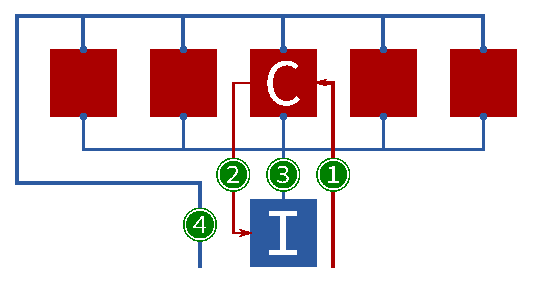
\includegraphics[width=\columnwidth]{../circuitry/spatial_pooler.pdf}
	\end{center}
	\caption{Timing based implementation of the spatial pooler. Each column is represented by a single cell \emph{C} and receives sparse input from the input vector \protect\circled{green}{1}. The columns become active when the number of connected active inputs crosses a threshold. The rise time of the membrane voltage highly depends on the number of coincident inputs: cells with more presynaptic activity will fire before those with less stimuli do. Inhibitory pool \emph{I} accumulates the columnar spikes \protect\circled{green}{2} and in doing so acts as a counter. After a certain number of columns have become active, the pool will inhibit and shut down all columns preventing any further activity \protect\circled{green}{3}. To stabilize this \gls{kwta} model, all columns receive a subsampled feed-forward inhibition \protect\circled{green}{4}. This effectively prolongs the decision period for high input activity.}
	\label{fig:spatial_pooler}
\end{figure}

At its core the spatial pooler resembles a \gls{kwta} network: $k$ out of $m$ columns are chosen to be active in each time step. In fact, \gls{kwta} networks have often been mentioned as an approximation for circuits naturally occurring in the neocortex \citep{felch2008hypergeometric}. While this topic has been discussed broadly in literature and continuous-time as well as VLSI implementations were investigated \citep{erlanson1991analog,tymoshchuk2012,maass2000neural}, the requirements which lead to this particular solution go beyond the discussed network architectures.

The network developed for this purpose is presented in figure~\ref{fig:spatial_pooler}. It follows a purely timing-based approach and is designed for \gls{lif} neurons. It allows for very fast decision processes based on a single input event per source. Each column is represented by a single cell which accumulates feed-forward input from the spike sources. Here, the rise time of the membrane voltage decreases with the number of presynaptic events seen by the cell: cells receiving the most input will fire before the others. An inhibitory pool consisting of a single cell collects the network's activity. Low membrane and high synaptic time constants lead to a reliable summation of events. When a certain number of spikes have been collected -- and thus the cell's threshold has been crossed --, the pool strongly inhibits all cells of the network suppressing following spike events.

The model is extended by adding subtle feed-forward shunting inhibition. The inhibitory conductance increases with the overall input activity $\nu_\text{in}$. With the reversal potential set to match the leakage potential, the conductance contributes to the leakage term

\begin{align*}
	g_\text{l}' &= g_\text{l} + g_\text{inh}(\nu_\text{in}).
\end{align*}
%
thus increasing the membrane time constant. This effectively slows down the neurons' responses and thus prolongs the decision period of the network.

Tie situations between columns receiving the same number of presynaptic events can be resolved by adding slight gaussian jitter to the weights of the excitatory feed-forward connections. This gives some columns structural advantages over other columns resulting in a slightly faster response to the same stimulus. By increasing the standard deviation $\sigma_\text{j}$ of the jitter, the selection criterion can be blurred.

%The proposed \gls{kwta} architecture was developed with the spatial pooler's properties in mind. In the following paragraphs, the model's performance is examined and compared to the goals formulated in section~\ref{sec:spatial_pooler_properties}.

\subsection{Temporal Memory}

Similar to the spatial pooler, the temporal memory implementation was designed for fast reaction times and spike-timing based response patterns. A complete network consists of $m$ identical columns with $n$ \gls{htm} cells each. Modelling these cells is a challenge in itself. A multicompartmental neuron model would represent the best fit. While a neuromorphic hardware chip implementing such a model is planned and first steps in that direction have already been taken \citep{millner2012development}, the current system does not provide this feature. Since \gls{htm} cells primarily depend on the active properties of a compartment, it can be modelled by a triple of individual \gls{lif} cells as shown in figure~\ref{fig:temporal_memory}.

\begin{figure}
	\begin{center}
		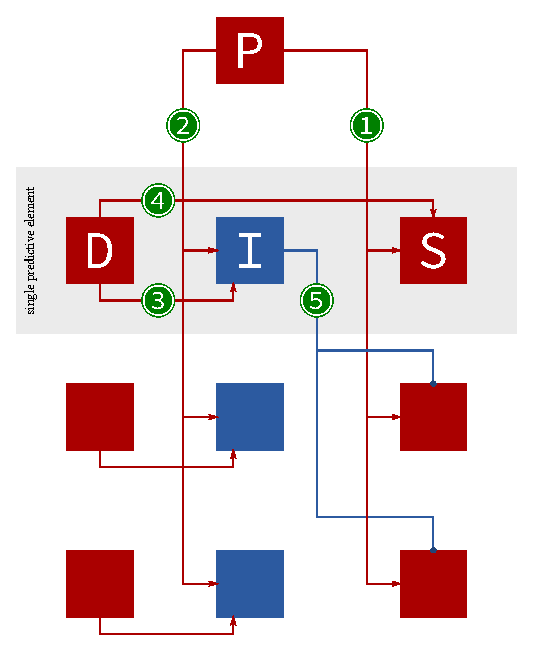
\includegraphics[width=\columnwidth]{../circuitry/column.pdf}
	\end{center}
	\caption{Implementation of the temporal memory not including plasticity. Every HTM cell within a column is modeled with three individual LIF cells modeling different compartments (distal dendrites \emph{D}, soma \emph{S} and a lateral inhibition segment \emph{I} -- which is not biologically inspired). Per column, there exist multiple cell triples as well as one ``head'' cell \emph{P} which participates in the columnar competition and collects proximal input for the whole column. Activity of this cell is forwarded to the individual soma cells of the column \protect\circled{green}{1}. Without a previous prediction, this results in all soma cells firing. However, the distal compartment sums over the input of the previous time step. When a threshold is reached, the inhibitory compartment as well as the soma are depolarized \protect\circled{green}{3} \protect\circled{green}{4}. Together with proximal input \protect\circled{green}{2}, the inhibitory partition fires and inhibits all other cells in the column \protect\circled{green}{5}.}
	\label{fig:temporal_memory}
\end{figure}

A column collects proximal input using a single cell. In fact, this cell can be part of a spatial pooler network as presented in section~\ref{sss:spatial_pooler_network}. When the column becomes active, this cell emits a spike and excites both the neurons representing the \gls{htm} cells' somae as well as inhibitory cells. The latter projection, however, is not strong enough to activate the target compartment alone. Instead, it only leads to a partial depolarization. The soma neuron, however, reaches the firing threshold for a single presynaptic event. This suffices as a columnar bursting mechanism: without predictive input, all soma compartments will fire as a response to the proximal stimulus.

Distal input is processed for each cell individually by their dendritic segment compartments. A cell's dendritic segment receives input from other cells' somae. In case its firing threshold is crossed, it partly depolarizes the inhibitory helper cell of the same triplet. This synaptic projection is set up with a relatively long synaptic time constant and a reversal potential matching the threshold voltage. This ensures that the predictive state is carried to the next time step and prohibits the cell from becoming active due to distal input alone. On proximal input, the already depolarized helper cell fires before the somatic compartments. The latter are then inhibited instantly, with the exception of the own triplet's soma. This basic predictive mechanism fails when multiple cells are predicted, since the inhibitory compartments laterally inhibit every cell. By also depolarizing the somatic compartments of predicted cells, this issue can be solved.

\begin{figure*}[p]
	\begin{center}
		%% Creator: Matplotlib, PGF backend
%%
%% To include the figure in your LaTeX document, write
%%   \input{<filename>.pgf}
%%
%% Make sure the required packages are loaded in your preamble
%%   \usepackage{pgf}
%%
%% Figures using additional raster images can only be included by \input if
%% they are in the same directory as the main LaTeX file. For loading figures
%% from other directories you can use the `import` package
%%   \usepackage{import}
%% and then include the figures with
%%   \import{<path to file>}{<filename>.pgf}
%%
%% Matplotlib used the following preamble
%%   \usepackage{amsmath}
%%   \usepackage{pifont}
%%   \usepackage{xcolor}
%%   \definecolor{green}{HTML}{467821}
%%   \definecolor{red}{HTML}{CF4457}
%%   \usepackage{siunitx}
%%   \usepackage{unicode-math}
%%   \setmainfont{Linux Libertine}
%%   \setsansfont{Linux Libertine}
%%   \setmathfont[range=\mathit]{Linux Libertine Italic}
%%   \setmathfont{Linux Libertine}
%%   \usepackage{fontspec}
%%
\begingroup%
\makeatletter%
\begin{pgfpicture}%
\pgfpathrectangle{\pgfpointorigin}{\pgfqpoint{5.808402in}{7.004719in}}%
\pgfusepath{use as bounding box, clip}%
\begin{pgfscope}%
\pgfsetbuttcap%
\pgfsetmiterjoin%
\definecolor{currentfill}{rgb}{1.000000,1.000000,1.000000}%
\pgfsetfillcolor{currentfill}%
\pgfsetlinewidth{0.000000pt}%
\definecolor{currentstroke}{rgb}{1.000000,1.000000,1.000000}%
\pgfsetstrokecolor{currentstroke}%
\pgfsetdash{}{0pt}%
\pgfpathmoveto{\pgfqpoint{0.000000in}{-0.000000in}}%
\pgfpathlineto{\pgfqpoint{5.808402in}{-0.000000in}}%
\pgfpathlineto{\pgfqpoint{5.808402in}{7.004719in}}%
\pgfpathlineto{\pgfqpoint{0.000000in}{7.004719in}}%
\pgfpathclose%
\pgfusepath{fill}%
\end{pgfscope}%
\begin{pgfscope}%
\pgfsetbuttcap%
\pgfsetmiterjoin%
\definecolor{currentfill}{rgb}{1.000000,1.000000,1.000000}%
\pgfsetfillcolor{currentfill}%
\pgfsetlinewidth{0.000000pt}%
\definecolor{currentstroke}{rgb}{0.000000,0.000000,0.000000}%
\pgfsetstrokecolor{currentstroke}%
\pgfsetstrokeopacity{0.000000}%
\pgfsetdash{}{0pt}%
\pgfpathmoveto{\pgfqpoint{0.512732in}{6.169547in}}%
\pgfpathlineto{\pgfqpoint{5.627732in}{6.169547in}}%
\pgfpathlineto{\pgfqpoint{5.627732in}{6.738297in}}%
\pgfpathlineto{\pgfqpoint{0.512732in}{6.738297in}}%
\pgfpathclose%
\pgfusepath{fill}%
\end{pgfscope}%
\begin{pgfscope}%
\pgfsetbuttcap%
\pgfsetroundjoin%
\definecolor{currentfill}{rgb}{0.333333,0.333333,0.333333}%
\pgfsetfillcolor{currentfill}%
\pgfsetlinewidth{0.501875pt}%
\definecolor{currentstroke}{rgb}{0.333333,0.333333,0.333333}%
\pgfsetstrokecolor{currentstroke}%
\pgfsetdash{}{0pt}%
\pgfsys@defobject{currentmarker}{\pgfqpoint{0.000000in}{0.000000in}}{\pgfqpoint{0.000000in}{0.000000in}}{%
\pgfpathmoveto{\pgfqpoint{0.000000in}{0.000000in}}%
\pgfpathlineto{\pgfqpoint{0.000000in}{0.000000in}}%
\pgfusepath{stroke,fill}%
}%
\begin{pgfscope}%
\pgfsys@transformshift{0.512732in}{6.216943in}%
\pgfsys@useobject{currentmarker}{}%
\end{pgfscope}%
\end{pgfscope}%
\begin{pgfscope}%
\pgfsetbuttcap%
\pgfsetroundjoin%
\definecolor{currentfill}{rgb}{0.333333,0.333333,0.333333}%
\pgfsetfillcolor{currentfill}%
\pgfsetlinewidth{0.501875pt}%
\definecolor{currentstroke}{rgb}{0.333333,0.333333,0.333333}%
\pgfsetstrokecolor{currentstroke}%
\pgfsetdash{}{0pt}%
\pgfsys@defobject{currentmarker}{\pgfqpoint{0.000000in}{0.000000in}}{\pgfqpoint{0.000000in}{0.000000in}}{%
\pgfpathmoveto{\pgfqpoint{0.000000in}{0.000000in}}%
\pgfpathlineto{\pgfqpoint{0.000000in}{0.000000in}}%
\pgfusepath{stroke,fill}%
}%
\begin{pgfscope}%
\pgfsys@transformshift{5.627732in}{6.216943in}%
\pgfsys@useobject{currentmarker}{}%
\end{pgfscope}%
\end{pgfscope}%
\begin{pgfscope}%
\definecolor{textcolor}{rgb}{0.333333,0.333333,0.333333}%
\pgfsetstrokecolor{textcolor}%
\pgfsetfillcolor{textcolor}%
\pgftext[x=0.429399in,y=6.216943in,right,]{\color{textcolor}\sffamily\fontsize{8.330000}{9.996000}\selectfont \(\displaystyle -70\)}%
\end{pgfscope}%
\begin{pgfscope}%
\pgfsetbuttcap%
\pgfsetroundjoin%
\definecolor{currentfill}{rgb}{0.333333,0.333333,0.333333}%
\pgfsetfillcolor{currentfill}%
\pgfsetlinewidth{0.501875pt}%
\definecolor{currentstroke}{rgb}{0.333333,0.333333,0.333333}%
\pgfsetstrokecolor{currentstroke}%
\pgfsetdash{}{0pt}%
\pgfsys@defobject{currentmarker}{\pgfqpoint{0.000000in}{0.000000in}}{\pgfqpoint{0.000000in}{0.000000in}}{%
\pgfpathmoveto{\pgfqpoint{0.000000in}{0.000000in}}%
\pgfpathlineto{\pgfqpoint{0.000000in}{0.000000in}}%
\pgfusepath{stroke,fill}%
}%
\begin{pgfscope}%
\pgfsys@transformshift{0.512732in}{6.335432in}%
\pgfsys@useobject{currentmarker}{}%
\end{pgfscope}%
\end{pgfscope}%
\begin{pgfscope}%
\pgfsetbuttcap%
\pgfsetroundjoin%
\definecolor{currentfill}{rgb}{0.333333,0.333333,0.333333}%
\pgfsetfillcolor{currentfill}%
\pgfsetlinewidth{0.501875pt}%
\definecolor{currentstroke}{rgb}{0.333333,0.333333,0.333333}%
\pgfsetstrokecolor{currentstroke}%
\pgfsetdash{}{0pt}%
\pgfsys@defobject{currentmarker}{\pgfqpoint{0.000000in}{0.000000in}}{\pgfqpoint{0.000000in}{0.000000in}}{%
\pgfpathmoveto{\pgfqpoint{0.000000in}{0.000000in}}%
\pgfpathlineto{\pgfqpoint{0.000000in}{0.000000in}}%
\pgfusepath{stroke,fill}%
}%
\begin{pgfscope}%
\pgfsys@transformshift{5.627732in}{6.335432in}%
\pgfsys@useobject{currentmarker}{}%
\end{pgfscope}%
\end{pgfscope}%
\begin{pgfscope}%
\definecolor{textcolor}{rgb}{0.333333,0.333333,0.333333}%
\pgfsetstrokecolor{textcolor}%
\pgfsetfillcolor{textcolor}%
\pgftext[x=0.429399in,y=6.335432in,right,]{\color{textcolor}\sffamily\fontsize{8.330000}{9.996000}\selectfont \(\displaystyle -65\)}%
\end{pgfscope}%
\begin{pgfscope}%
\pgfsetbuttcap%
\pgfsetroundjoin%
\definecolor{currentfill}{rgb}{0.333333,0.333333,0.333333}%
\pgfsetfillcolor{currentfill}%
\pgfsetlinewidth{0.501875pt}%
\definecolor{currentstroke}{rgb}{0.333333,0.333333,0.333333}%
\pgfsetstrokecolor{currentstroke}%
\pgfsetdash{}{0pt}%
\pgfsys@defobject{currentmarker}{\pgfqpoint{0.000000in}{0.000000in}}{\pgfqpoint{0.000000in}{0.000000in}}{%
\pgfpathmoveto{\pgfqpoint{0.000000in}{0.000000in}}%
\pgfpathlineto{\pgfqpoint{0.000000in}{0.000000in}}%
\pgfusepath{stroke,fill}%
}%
\begin{pgfscope}%
\pgfsys@transformshift{0.512732in}{6.453922in}%
\pgfsys@useobject{currentmarker}{}%
\end{pgfscope}%
\end{pgfscope}%
\begin{pgfscope}%
\pgfsetbuttcap%
\pgfsetroundjoin%
\definecolor{currentfill}{rgb}{0.333333,0.333333,0.333333}%
\pgfsetfillcolor{currentfill}%
\pgfsetlinewidth{0.501875pt}%
\definecolor{currentstroke}{rgb}{0.333333,0.333333,0.333333}%
\pgfsetstrokecolor{currentstroke}%
\pgfsetdash{}{0pt}%
\pgfsys@defobject{currentmarker}{\pgfqpoint{0.000000in}{0.000000in}}{\pgfqpoint{0.000000in}{0.000000in}}{%
\pgfpathmoveto{\pgfqpoint{0.000000in}{0.000000in}}%
\pgfpathlineto{\pgfqpoint{0.000000in}{0.000000in}}%
\pgfusepath{stroke,fill}%
}%
\begin{pgfscope}%
\pgfsys@transformshift{5.627732in}{6.453922in}%
\pgfsys@useobject{currentmarker}{}%
\end{pgfscope}%
\end{pgfscope}%
\begin{pgfscope}%
\definecolor{textcolor}{rgb}{0.333333,0.333333,0.333333}%
\pgfsetstrokecolor{textcolor}%
\pgfsetfillcolor{textcolor}%
\pgftext[x=0.429399in,y=6.453922in,right,]{\color{textcolor}\sffamily\fontsize{8.330000}{9.996000}\selectfont \(\displaystyle -60\)}%
\end{pgfscope}%
\begin{pgfscope}%
\pgfsetbuttcap%
\pgfsetroundjoin%
\definecolor{currentfill}{rgb}{0.333333,0.333333,0.333333}%
\pgfsetfillcolor{currentfill}%
\pgfsetlinewidth{0.501875pt}%
\definecolor{currentstroke}{rgb}{0.333333,0.333333,0.333333}%
\pgfsetstrokecolor{currentstroke}%
\pgfsetdash{}{0pt}%
\pgfsys@defobject{currentmarker}{\pgfqpoint{0.000000in}{0.000000in}}{\pgfqpoint{0.000000in}{0.000000in}}{%
\pgfpathmoveto{\pgfqpoint{0.000000in}{0.000000in}}%
\pgfpathlineto{\pgfqpoint{0.000000in}{0.000000in}}%
\pgfusepath{stroke,fill}%
}%
\begin{pgfscope}%
\pgfsys@transformshift{0.512732in}{6.572411in}%
\pgfsys@useobject{currentmarker}{}%
\end{pgfscope}%
\end{pgfscope}%
\begin{pgfscope}%
\pgfsetbuttcap%
\pgfsetroundjoin%
\definecolor{currentfill}{rgb}{0.333333,0.333333,0.333333}%
\pgfsetfillcolor{currentfill}%
\pgfsetlinewidth{0.501875pt}%
\definecolor{currentstroke}{rgb}{0.333333,0.333333,0.333333}%
\pgfsetstrokecolor{currentstroke}%
\pgfsetdash{}{0pt}%
\pgfsys@defobject{currentmarker}{\pgfqpoint{0.000000in}{0.000000in}}{\pgfqpoint{0.000000in}{0.000000in}}{%
\pgfpathmoveto{\pgfqpoint{0.000000in}{0.000000in}}%
\pgfpathlineto{\pgfqpoint{0.000000in}{0.000000in}}%
\pgfusepath{stroke,fill}%
}%
\begin{pgfscope}%
\pgfsys@transformshift{5.627732in}{6.572411in}%
\pgfsys@useobject{currentmarker}{}%
\end{pgfscope}%
\end{pgfscope}%
\begin{pgfscope}%
\definecolor{textcolor}{rgb}{0.333333,0.333333,0.333333}%
\pgfsetstrokecolor{textcolor}%
\pgfsetfillcolor{textcolor}%
\pgftext[x=0.429399in,y=6.572411in,right,]{\color{textcolor}\sffamily\fontsize{8.330000}{9.996000}\selectfont \(\displaystyle -55\)}%
\end{pgfscope}%
\begin{pgfscope}%
\pgfsetbuttcap%
\pgfsetroundjoin%
\definecolor{currentfill}{rgb}{0.333333,0.333333,0.333333}%
\pgfsetfillcolor{currentfill}%
\pgfsetlinewidth{0.501875pt}%
\definecolor{currentstroke}{rgb}{0.333333,0.333333,0.333333}%
\pgfsetstrokecolor{currentstroke}%
\pgfsetdash{}{0pt}%
\pgfsys@defobject{currentmarker}{\pgfqpoint{0.000000in}{0.000000in}}{\pgfqpoint{0.000000in}{0.000000in}}{%
\pgfpathmoveto{\pgfqpoint{0.000000in}{0.000000in}}%
\pgfpathlineto{\pgfqpoint{0.000000in}{0.000000in}}%
\pgfusepath{stroke,fill}%
}%
\begin{pgfscope}%
\pgfsys@transformshift{0.512732in}{6.690901in}%
\pgfsys@useobject{currentmarker}{}%
\end{pgfscope}%
\end{pgfscope}%
\begin{pgfscope}%
\pgfsetbuttcap%
\pgfsetroundjoin%
\definecolor{currentfill}{rgb}{0.333333,0.333333,0.333333}%
\pgfsetfillcolor{currentfill}%
\pgfsetlinewidth{0.501875pt}%
\definecolor{currentstroke}{rgb}{0.333333,0.333333,0.333333}%
\pgfsetstrokecolor{currentstroke}%
\pgfsetdash{}{0pt}%
\pgfsys@defobject{currentmarker}{\pgfqpoint{0.000000in}{0.000000in}}{\pgfqpoint{0.000000in}{0.000000in}}{%
\pgfpathmoveto{\pgfqpoint{0.000000in}{0.000000in}}%
\pgfpathlineto{\pgfqpoint{0.000000in}{0.000000in}}%
\pgfusepath{stroke,fill}%
}%
\begin{pgfscope}%
\pgfsys@transformshift{5.627732in}{6.690901in}%
\pgfsys@useobject{currentmarker}{}%
\end{pgfscope}%
\end{pgfscope}%
\begin{pgfscope}%
\definecolor{textcolor}{rgb}{0.333333,0.333333,0.333333}%
\pgfsetstrokecolor{textcolor}%
\pgfsetfillcolor{textcolor}%
\pgftext[x=0.429399in,y=6.690901in,right,]{\color{textcolor}\sffamily\fontsize{8.330000}{9.996000}\selectfont \(\displaystyle -50\)}%
\end{pgfscope}%
\begin{pgfscope}%
\definecolor{textcolor}{rgb}{0.333333,0.333333,0.333333}%
\pgfsetstrokecolor{textcolor}%
\pgfsetfillcolor{textcolor}%
\pgftext[x=0.188786in,y=6.453922in,,bottom,rotate=90.000000]{\color{textcolor}\sffamily\fontsize{6.000000}{7.200000}\selectfont \(\displaystyle V_\text{distal}\) [\si{\milli\volt}]}%
\end{pgfscope}%
\begin{pgfscope}%
\pgfpathrectangle{\pgfqpoint{0.512732in}{6.169547in}}{\pgfqpoint{5.115000in}{0.568750in}} %
\pgfusepath{clip}%
\pgfsetbuttcap%
\pgfsetmiterjoin%
\definecolor{currentfill}{rgb}{0.827451,0.827451,0.827451}%
\pgfsetfillcolor{currentfill}%
\pgfsetfillopacity{0.500000}%
\pgfsetlinewidth{0.501875pt}%
\definecolor{currentstroke}{rgb}{0.933333,0.933333,0.933333}%
\pgfsetstrokecolor{currentstroke}%
\pgfsetstrokeopacity{0.500000}%
\pgfsetdash{}{0pt}%
\pgfpathmoveto{\pgfqpoint{0.512732in}{6.169547in}}%
\pgfpathlineto{\pgfqpoint{0.512732in}{6.738297in}}%
\pgfpathlineto{\pgfqpoint{1.152107in}{6.738297in}}%
\pgfpathlineto{\pgfqpoint{1.152107in}{6.169547in}}%
\pgfpathlineto{\pgfqpoint{0.512732in}{6.169547in}}%
\pgfusepath{stroke,fill}%
\end{pgfscope}%
\begin{pgfscope}%
\pgfpathrectangle{\pgfqpoint{0.512732in}{6.169547in}}{\pgfqpoint{5.115000in}{0.568750in}} %
\pgfusepath{clip}%
\pgfsetbuttcap%
\pgfsetmiterjoin%
\definecolor{currentfill}{rgb}{0.827451,0.827451,0.827451}%
\pgfsetfillcolor{currentfill}%
\pgfsetfillopacity{0.500000}%
\pgfsetlinewidth{0.501875pt}%
\definecolor{currentstroke}{rgb}{0.933333,0.933333,0.933333}%
\pgfsetstrokecolor{currentstroke}%
\pgfsetstrokeopacity{0.500000}%
\pgfsetdash{}{0pt}%
\pgfpathmoveto{\pgfqpoint{3.709607in}{6.169547in}}%
\pgfpathlineto{\pgfqpoint{3.709607in}{6.738297in}}%
\pgfpathlineto{\pgfqpoint{4.348982in}{6.738297in}}%
\pgfpathlineto{\pgfqpoint{4.348982in}{6.169547in}}%
\pgfpathlineto{\pgfqpoint{3.709607in}{6.169547in}}%
\pgfusepath{stroke,fill}%
\end{pgfscope}%
\begin{pgfscope}%
\pgfpathrectangle{\pgfqpoint{0.512732in}{6.169547in}}{\pgfqpoint{5.115000in}{0.568750in}} %
\pgfusepath{clip}%
\pgfsetbuttcap%
\pgfsetmiterjoin%
\definecolor{currentfill}{rgb}{0.827451,0.827451,0.827451}%
\pgfsetfillcolor{currentfill}%
\pgfsetfillopacity{0.500000}%
\pgfsetlinewidth{0.501875pt}%
\definecolor{currentstroke}{rgb}{0.933333,0.933333,0.933333}%
\pgfsetstrokecolor{currentstroke}%
\pgfsetstrokeopacity{0.500000}%
\pgfsetdash{}{0pt}%
\pgfpathmoveto{\pgfqpoint{4.348982in}{6.169547in}}%
\pgfpathlineto{\pgfqpoint{4.348982in}{6.738297in}}%
\pgfpathlineto{\pgfqpoint{4.988357in}{6.738297in}}%
\pgfpathlineto{\pgfqpoint{4.988357in}{6.169547in}}%
\pgfpathlineto{\pgfqpoint{4.348982in}{6.169547in}}%
\pgfusepath{stroke,fill}%
\end{pgfscope}%
\begin{pgfscope}%
\pgfpathrectangle{\pgfqpoint{0.512732in}{6.169547in}}{\pgfqpoint{5.115000in}{0.568750in}} %
\pgfusepath{clip}%
\pgfsetrectcap%
\pgfsetroundjoin%
\pgfsetlinewidth{0.501875pt}%
\definecolor{currentstroke}{rgb}{0.827451,0.827451,0.827451}%
\pgfsetstrokecolor{currentstroke}%
\pgfsetdash{}{0pt}%
\pgfpathmoveto{\pgfqpoint{0.512732in}{6.169547in}}%
\pgfpathlineto{\pgfqpoint{0.512732in}{6.738297in}}%
\pgfusepath{stroke}%
\end{pgfscope}%
\begin{pgfscope}%
\pgfpathrectangle{\pgfqpoint{0.512732in}{6.169547in}}{\pgfqpoint{5.115000in}{0.568750in}} %
\pgfusepath{clip}%
\pgfsetrectcap%
\pgfsetroundjoin%
\pgfsetlinewidth{0.501875pt}%
\definecolor{currentstroke}{rgb}{0.827451,0.827451,0.827451}%
\pgfsetstrokecolor{currentstroke}%
\pgfsetdash{}{0pt}%
\pgfpathmoveto{\pgfqpoint{1.152107in}{6.169547in}}%
\pgfpathlineto{\pgfqpoint{1.152107in}{6.738297in}}%
\pgfusepath{stroke}%
\end{pgfscope}%
\begin{pgfscope}%
\pgfpathrectangle{\pgfqpoint{0.512732in}{6.169547in}}{\pgfqpoint{5.115000in}{0.568750in}} %
\pgfusepath{clip}%
\pgfsetrectcap%
\pgfsetroundjoin%
\pgfsetlinewidth{0.501875pt}%
\definecolor{currentstroke}{rgb}{0.827451,0.827451,0.827451}%
\pgfsetstrokecolor{currentstroke}%
\pgfsetdash{}{0pt}%
\pgfpathmoveto{\pgfqpoint{1.791482in}{6.169547in}}%
\pgfpathlineto{\pgfqpoint{1.791482in}{6.738297in}}%
\pgfusepath{stroke}%
\end{pgfscope}%
\begin{pgfscope}%
\pgfpathrectangle{\pgfqpoint{0.512732in}{6.169547in}}{\pgfqpoint{5.115000in}{0.568750in}} %
\pgfusepath{clip}%
\pgfsetrectcap%
\pgfsetroundjoin%
\pgfsetlinewidth{0.501875pt}%
\definecolor{currentstroke}{rgb}{0.827451,0.827451,0.827451}%
\pgfsetstrokecolor{currentstroke}%
\pgfsetdash{}{0pt}%
\pgfpathmoveto{\pgfqpoint{2.430857in}{6.169547in}}%
\pgfpathlineto{\pgfqpoint{2.430857in}{6.738297in}}%
\pgfusepath{stroke}%
\end{pgfscope}%
\begin{pgfscope}%
\pgfpathrectangle{\pgfqpoint{0.512732in}{6.169547in}}{\pgfqpoint{5.115000in}{0.568750in}} %
\pgfusepath{clip}%
\pgfsetrectcap%
\pgfsetroundjoin%
\pgfsetlinewidth{0.501875pt}%
\definecolor{currentstroke}{rgb}{0.827451,0.827451,0.827451}%
\pgfsetstrokecolor{currentstroke}%
\pgfsetdash{}{0pt}%
\pgfpathmoveto{\pgfqpoint{3.070232in}{6.169547in}}%
\pgfpathlineto{\pgfqpoint{3.070232in}{6.738297in}}%
\pgfusepath{stroke}%
\end{pgfscope}%
\begin{pgfscope}%
\pgfpathrectangle{\pgfqpoint{0.512732in}{6.169547in}}{\pgfqpoint{5.115000in}{0.568750in}} %
\pgfusepath{clip}%
\pgfsetrectcap%
\pgfsetroundjoin%
\pgfsetlinewidth{0.501875pt}%
\definecolor{currentstroke}{rgb}{0.827451,0.827451,0.827451}%
\pgfsetstrokecolor{currentstroke}%
\pgfsetdash{}{0pt}%
\pgfpathmoveto{\pgfqpoint{3.709607in}{6.169547in}}%
\pgfpathlineto{\pgfqpoint{3.709607in}{6.738297in}}%
\pgfusepath{stroke}%
\end{pgfscope}%
\begin{pgfscope}%
\pgfpathrectangle{\pgfqpoint{0.512732in}{6.169547in}}{\pgfqpoint{5.115000in}{0.568750in}} %
\pgfusepath{clip}%
\pgfsetrectcap%
\pgfsetroundjoin%
\pgfsetlinewidth{0.501875pt}%
\definecolor{currentstroke}{rgb}{0.827451,0.827451,0.827451}%
\pgfsetstrokecolor{currentstroke}%
\pgfsetdash{}{0pt}%
\pgfpathmoveto{\pgfqpoint{4.348982in}{6.169547in}}%
\pgfpathlineto{\pgfqpoint{4.348982in}{6.738297in}}%
\pgfusepath{stroke}%
\end{pgfscope}%
\begin{pgfscope}%
\pgfpathrectangle{\pgfqpoint{0.512732in}{6.169547in}}{\pgfqpoint{5.115000in}{0.568750in}} %
\pgfusepath{clip}%
\pgfsetrectcap%
\pgfsetroundjoin%
\pgfsetlinewidth{0.501875pt}%
\definecolor{currentstroke}{rgb}{0.827451,0.827451,0.827451}%
\pgfsetstrokecolor{currentstroke}%
\pgfsetdash{}{0pt}%
\pgfpathmoveto{\pgfqpoint{4.988357in}{6.169547in}}%
\pgfpathlineto{\pgfqpoint{4.988357in}{6.738297in}}%
\pgfusepath{stroke}%
\end{pgfscope}%
\begin{pgfscope}%
\pgfpathrectangle{\pgfqpoint{0.512732in}{6.169547in}}{\pgfqpoint{5.115000in}{0.568750in}} %
\pgfusepath{clip}%
\pgfsetrectcap%
\pgfsetroundjoin%
\pgfsetlinewidth{0.803000pt}%
\definecolor{currentstroke}{rgb}{0.203922,0.541176,0.741176}%
\pgfsetstrokecolor{currentstroke}%
\pgfsetdash{}{0pt}%
\pgfpathmoveto{\pgfqpoint{0.512732in}{6.335432in}}%
\pgfpathlineto{\pgfqpoint{0.577949in}{6.335432in}}%
\pgfpathlineto{\pgfqpoint{0.579227in}{6.339224in}}%
\pgfpathlineto{\pgfqpoint{0.581785in}{6.357637in}}%
\pgfpathlineto{\pgfqpoint{0.590736in}{6.447144in}}%
\pgfpathlineto{\pgfqpoint{0.599687in}{6.516105in}}%
\pgfpathlineto{\pgfqpoint{0.608639in}{6.569354in}}%
\pgfpathlineto{\pgfqpoint{0.617590in}{6.610447in}}%
\pgfpathlineto{\pgfqpoint{0.626541in}{6.642036in}}%
\pgfpathlineto{\pgfqpoint{0.635492in}{6.666089in}}%
\pgfpathlineto{\pgfqpoint{0.644444in}{6.684147in}}%
\pgfpathlineto{\pgfqpoint{0.648280in}{6.690356in}}%
\pgfpathlineto{\pgfqpoint{0.649559in}{6.216943in}}%
\pgfpathlineto{\pgfqpoint{0.662346in}{6.216943in}}%
\pgfpathlineto{\pgfqpoint{0.673855in}{6.246470in}}%
\pgfpathlineto{\pgfqpoint{0.685364in}{6.269552in}}%
\pgfpathlineto{\pgfqpoint{0.696872in}{6.287610in}}%
\pgfpathlineto{\pgfqpoint{0.708381in}{6.301757in}}%
\pgfpathlineto{\pgfqpoint{0.721169in}{6.313915in}}%
\pgfpathlineto{\pgfqpoint{0.735235in}{6.323986in}}%
\pgfpathlineto{\pgfqpoint{0.750580in}{6.331972in}}%
\pgfpathlineto{\pgfqpoint{0.768482in}{6.338442in}}%
\pgfpathlineto{\pgfqpoint{0.790221in}{6.343442in}}%
\pgfpathlineto{\pgfqpoint{0.817075in}{6.346831in}}%
\pgfpathlineto{\pgfqpoint{0.846486in}{6.348466in}}%
\pgfpathlineto{\pgfqpoint{0.887406in}{6.348893in}}%
\pgfpathlineto{\pgfqpoint{1.512715in}{6.338394in}}%
\pgfpathlineto{\pgfqpoint{1.691740in}{6.337304in}}%
\pgfpathlineto{\pgfqpoint{1.769744in}{6.336949in}}%
\pgfpathlineto{\pgfqpoint{2.267177in}{6.335859in}}%
\pgfpathlineto{\pgfqpoint{2.329836in}{6.335788in}}%
\pgfpathlineto{\pgfqpoint{3.774824in}{6.335432in}}%
\pgfpathlineto{\pgfqpoint{3.776102in}{6.339224in}}%
\pgfpathlineto{\pgfqpoint{3.778660in}{6.357637in}}%
\pgfpathlineto{\pgfqpoint{3.787611in}{6.447168in}}%
\pgfpathlineto{\pgfqpoint{3.796562in}{6.516105in}}%
\pgfpathlineto{\pgfqpoint{3.805514in}{6.569354in}}%
\pgfpathlineto{\pgfqpoint{3.814465in}{6.610447in}}%
\pgfpathlineto{\pgfqpoint{3.823416in}{6.642036in}}%
\pgfpathlineto{\pgfqpoint{3.832367in}{6.666089in}}%
\pgfpathlineto{\pgfqpoint{3.841319in}{6.684147in}}%
\pgfpathlineto{\pgfqpoint{3.845155in}{6.690356in}}%
\pgfpathlineto{\pgfqpoint{3.846434in}{6.216943in}}%
\pgfpathlineto{\pgfqpoint{3.859221in}{6.216943in}}%
\pgfpathlineto{\pgfqpoint{3.870730in}{6.246470in}}%
\pgfpathlineto{\pgfqpoint{3.882239in}{6.269552in}}%
\pgfpathlineto{\pgfqpoint{3.893747in}{6.287610in}}%
\pgfpathlineto{\pgfqpoint{3.905256in}{6.301757in}}%
\pgfpathlineto{\pgfqpoint{3.918044in}{6.313915in}}%
\pgfpathlineto{\pgfqpoint{3.932110in}{6.323986in}}%
\pgfpathlineto{\pgfqpoint{3.947455in}{6.331972in}}%
\pgfpathlineto{\pgfqpoint{3.965357in}{6.338442in}}%
\pgfpathlineto{\pgfqpoint{3.987096in}{6.343442in}}%
\pgfpathlineto{\pgfqpoint{4.013950in}{6.346831in}}%
\pgfpathlineto{\pgfqpoint{4.043361in}{6.348466in}}%
\pgfpathlineto{\pgfqpoint{4.084281in}{6.348893in}}%
\pgfpathlineto{\pgfqpoint{4.414199in}{6.341854in}}%
\pgfpathlineto{\pgfqpoint{4.415477in}{6.345599in}}%
\pgfpathlineto{\pgfqpoint{4.418035in}{6.363893in}}%
\pgfpathlineto{\pgfqpoint{4.426986in}{6.452903in}}%
\pgfpathlineto{\pgfqpoint{4.435937in}{6.521437in}}%
\pgfpathlineto{\pgfqpoint{4.444889in}{6.574331in}}%
\pgfpathlineto{\pgfqpoint{4.453840in}{6.615139in}}%
\pgfpathlineto{\pgfqpoint{4.462791in}{6.646491in}}%
\pgfpathlineto{\pgfqpoint{4.471742in}{6.670331in}}%
\pgfpathlineto{\pgfqpoint{4.480694in}{6.688199in}}%
\pgfpathlineto{\pgfqpoint{4.481972in}{6.690332in}}%
\pgfpathlineto{\pgfqpoint{4.483251in}{6.216943in}}%
\pgfpathlineto{\pgfqpoint{4.496039in}{6.216943in}}%
\pgfpathlineto{\pgfqpoint{4.507547in}{6.247797in}}%
\pgfpathlineto{\pgfqpoint{4.519056in}{6.271851in}}%
\pgfpathlineto{\pgfqpoint{4.530565in}{6.290643in}}%
\pgfpathlineto{\pgfqpoint{4.542074in}{6.305336in}}%
\pgfpathlineto{\pgfqpoint{4.554861in}{6.317919in}}%
\pgfpathlineto{\pgfqpoint{4.568927in}{6.328275in}}%
\pgfpathlineto{\pgfqpoint{4.584272in}{6.336451in}}%
\pgfpathlineto{\pgfqpoint{4.600896in}{6.342636in}}%
\pgfpathlineto{\pgfqpoint{4.621356in}{6.347566in}}%
\pgfpathlineto{\pgfqpoint{4.644374in}{6.350741in}}%
\pgfpathlineto{\pgfqpoint{4.676342in}{6.352637in}}%
\pgfpathlineto{\pgfqpoint{4.732607in}{6.352590in}}%
\pgfpathlineto{\pgfqpoint{4.827235in}{6.349746in}}%
\pgfpathlineto{\pgfqpoint{4.979406in}{6.345196in}}%
\pgfpathlineto{\pgfqpoint{5.379655in}{6.338868in}}%
\pgfpathlineto{\pgfqpoint{5.527990in}{6.337778in}}%
\pgfpathlineto{\pgfqpoint{5.612387in}{6.337304in}}%
\pgfpathlineto{\pgfqpoint{5.627732in}{6.337233in}}%
\pgfpathlineto{\pgfqpoint{5.627732in}{6.337233in}}%
\pgfusepath{stroke}%
\end{pgfscope}%
\begin{pgfscope}%
\pgfpathrectangle{\pgfqpoint{0.512732in}{6.169547in}}{\pgfqpoint{5.115000in}{0.568750in}} %
\pgfusepath{clip}%
\pgfsetrectcap%
\pgfsetroundjoin%
\pgfsetlinewidth{0.803000pt}%
\definecolor{currentstroke}{rgb}{0.478431,0.407843,0.650980}%
\pgfsetstrokecolor{currentstroke}%
\pgfsetdash{}{0pt}%
\pgfpathmoveto{\pgfqpoint{0.512732in}{6.335432in}}%
\pgfpathlineto{\pgfqpoint{5.627732in}{6.335432in}}%
\pgfpathlineto{\pgfqpoint{5.627732in}{6.335432in}}%
\pgfusepath{stroke}%
\end{pgfscope}%
\begin{pgfscope}%
\pgfsetrectcap%
\pgfsetmiterjoin%
\pgfsetlinewidth{0.501875pt}%
\definecolor{currentstroke}{rgb}{0.690196,0.690196,0.690196}%
\pgfsetstrokecolor{currentstroke}%
\pgfsetdash{}{0pt}%
\pgfpathmoveto{\pgfqpoint{0.512732in}{6.738297in}}%
\pgfpathlineto{\pgfqpoint{5.627732in}{6.738297in}}%
\pgfusepath{stroke}%
\end{pgfscope}%
\begin{pgfscope}%
\pgfsetrectcap%
\pgfsetmiterjoin%
\pgfsetlinewidth{0.501875pt}%
\definecolor{currentstroke}{rgb}{0.690196,0.690196,0.690196}%
\pgfsetstrokecolor{currentstroke}%
\pgfsetdash{}{0pt}%
\pgfpathmoveto{\pgfqpoint{5.627732in}{6.169547in}}%
\pgfpathlineto{\pgfqpoint{5.627732in}{6.738297in}}%
\pgfusepath{stroke}%
\end{pgfscope}%
\begin{pgfscope}%
\pgfsetrectcap%
\pgfsetmiterjoin%
\pgfsetlinewidth{0.501875pt}%
\definecolor{currentstroke}{rgb}{0.690196,0.690196,0.690196}%
\pgfsetstrokecolor{currentstroke}%
\pgfsetdash{}{0pt}%
\pgfpathmoveto{\pgfqpoint{0.512732in}{6.169547in}}%
\pgfpathlineto{\pgfqpoint{5.627732in}{6.169547in}}%
\pgfusepath{stroke}%
\end{pgfscope}%
\begin{pgfscope}%
\pgfsetrectcap%
\pgfsetmiterjoin%
\pgfsetlinewidth{0.501875pt}%
\definecolor{currentstroke}{rgb}{0.690196,0.690196,0.690196}%
\pgfsetstrokecolor{currentstroke}%
\pgfsetdash{}{0pt}%
\pgfpathmoveto{\pgfqpoint{0.512732in}{6.169547in}}%
\pgfpathlineto{\pgfqpoint{0.512732in}{6.738297in}}%
\pgfusepath{stroke}%
\end{pgfscope}%
\begin{pgfscope}%
\pgftext[x=3.070232in,y=6.807741in,,base]{\sffamily\fontsize{10.000000}{12.000000}\selectfont Cell 1}%
\end{pgfscope}%
\begin{pgfscope}%
\pgfsetbuttcap%
\pgfsetmiterjoin%
\definecolor{currentfill}{rgb}{1.000000,1.000000,1.000000}%
\pgfsetfillcolor{currentfill}%
\pgfsetlinewidth{0.000000pt}%
\definecolor{currentstroke}{rgb}{0.000000,0.000000,0.000000}%
\pgfsetstrokecolor{currentstroke}%
\pgfsetstrokeopacity{0.000000}%
\pgfsetdash{}{0pt}%
\pgfpathmoveto{\pgfqpoint{0.512732in}{4.918297in}}%
\pgfpathlineto{\pgfqpoint{5.627732in}{4.918297in}}%
\pgfpathlineto{\pgfqpoint{5.627732in}{5.487047in}}%
\pgfpathlineto{\pgfqpoint{0.512732in}{5.487047in}}%
\pgfpathclose%
\pgfusepath{fill}%
\end{pgfscope}%
\begin{pgfscope}%
\pgfsetbuttcap%
\pgfsetroundjoin%
\definecolor{currentfill}{rgb}{0.333333,0.333333,0.333333}%
\pgfsetfillcolor{currentfill}%
\pgfsetlinewidth{0.501875pt}%
\definecolor{currentstroke}{rgb}{0.333333,0.333333,0.333333}%
\pgfsetstrokecolor{currentstroke}%
\pgfsetdash{}{0pt}%
\pgfsys@defobject{currentmarker}{\pgfqpoint{0.000000in}{0.000000in}}{\pgfqpoint{0.000000in}{0.000000in}}{%
\pgfpathmoveto{\pgfqpoint{0.000000in}{0.000000in}}%
\pgfpathlineto{\pgfqpoint{0.000000in}{0.000000in}}%
\pgfusepath{stroke,fill}%
}%
\begin{pgfscope}%
\pgfsys@transformshift{0.512732in}{4.965693in}%
\pgfsys@useobject{currentmarker}{}%
\end{pgfscope}%
\end{pgfscope}%
\begin{pgfscope}%
\pgfsetbuttcap%
\pgfsetroundjoin%
\definecolor{currentfill}{rgb}{0.333333,0.333333,0.333333}%
\pgfsetfillcolor{currentfill}%
\pgfsetlinewidth{0.501875pt}%
\definecolor{currentstroke}{rgb}{0.333333,0.333333,0.333333}%
\pgfsetstrokecolor{currentstroke}%
\pgfsetdash{}{0pt}%
\pgfsys@defobject{currentmarker}{\pgfqpoint{0.000000in}{0.000000in}}{\pgfqpoint{0.000000in}{0.000000in}}{%
\pgfpathmoveto{\pgfqpoint{0.000000in}{0.000000in}}%
\pgfpathlineto{\pgfqpoint{0.000000in}{0.000000in}}%
\pgfusepath{stroke,fill}%
}%
\begin{pgfscope}%
\pgfsys@transformshift{5.627732in}{4.965693in}%
\pgfsys@useobject{currentmarker}{}%
\end{pgfscope}%
\end{pgfscope}%
\begin{pgfscope}%
\definecolor{textcolor}{rgb}{0.333333,0.333333,0.333333}%
\pgfsetstrokecolor{textcolor}%
\pgfsetfillcolor{textcolor}%
\pgftext[x=0.429399in,y=4.965693in,right,]{\color{textcolor}\sffamily\fontsize{8.330000}{9.996000}\selectfont \(\displaystyle -70\)}%
\end{pgfscope}%
\begin{pgfscope}%
\pgfsetbuttcap%
\pgfsetroundjoin%
\definecolor{currentfill}{rgb}{0.333333,0.333333,0.333333}%
\pgfsetfillcolor{currentfill}%
\pgfsetlinewidth{0.501875pt}%
\definecolor{currentstroke}{rgb}{0.333333,0.333333,0.333333}%
\pgfsetstrokecolor{currentstroke}%
\pgfsetdash{}{0pt}%
\pgfsys@defobject{currentmarker}{\pgfqpoint{0.000000in}{0.000000in}}{\pgfqpoint{0.000000in}{0.000000in}}{%
\pgfpathmoveto{\pgfqpoint{0.000000in}{0.000000in}}%
\pgfpathlineto{\pgfqpoint{0.000000in}{0.000000in}}%
\pgfusepath{stroke,fill}%
}%
\begin{pgfscope}%
\pgfsys@transformshift{0.512732in}{5.084182in}%
\pgfsys@useobject{currentmarker}{}%
\end{pgfscope}%
\end{pgfscope}%
\begin{pgfscope}%
\pgfsetbuttcap%
\pgfsetroundjoin%
\definecolor{currentfill}{rgb}{0.333333,0.333333,0.333333}%
\pgfsetfillcolor{currentfill}%
\pgfsetlinewidth{0.501875pt}%
\definecolor{currentstroke}{rgb}{0.333333,0.333333,0.333333}%
\pgfsetstrokecolor{currentstroke}%
\pgfsetdash{}{0pt}%
\pgfsys@defobject{currentmarker}{\pgfqpoint{0.000000in}{0.000000in}}{\pgfqpoint{0.000000in}{0.000000in}}{%
\pgfpathmoveto{\pgfqpoint{0.000000in}{0.000000in}}%
\pgfpathlineto{\pgfqpoint{0.000000in}{0.000000in}}%
\pgfusepath{stroke,fill}%
}%
\begin{pgfscope}%
\pgfsys@transformshift{5.627732in}{5.084182in}%
\pgfsys@useobject{currentmarker}{}%
\end{pgfscope}%
\end{pgfscope}%
\begin{pgfscope}%
\definecolor{textcolor}{rgb}{0.333333,0.333333,0.333333}%
\pgfsetstrokecolor{textcolor}%
\pgfsetfillcolor{textcolor}%
\pgftext[x=0.429399in,y=5.084182in,right,]{\color{textcolor}\sffamily\fontsize{8.330000}{9.996000}\selectfont \(\displaystyle -65\)}%
\end{pgfscope}%
\begin{pgfscope}%
\pgfsetbuttcap%
\pgfsetroundjoin%
\definecolor{currentfill}{rgb}{0.333333,0.333333,0.333333}%
\pgfsetfillcolor{currentfill}%
\pgfsetlinewidth{0.501875pt}%
\definecolor{currentstroke}{rgb}{0.333333,0.333333,0.333333}%
\pgfsetstrokecolor{currentstroke}%
\pgfsetdash{}{0pt}%
\pgfsys@defobject{currentmarker}{\pgfqpoint{0.000000in}{0.000000in}}{\pgfqpoint{0.000000in}{0.000000in}}{%
\pgfpathmoveto{\pgfqpoint{0.000000in}{0.000000in}}%
\pgfpathlineto{\pgfqpoint{0.000000in}{0.000000in}}%
\pgfusepath{stroke,fill}%
}%
\begin{pgfscope}%
\pgfsys@transformshift{0.512732in}{5.202672in}%
\pgfsys@useobject{currentmarker}{}%
\end{pgfscope}%
\end{pgfscope}%
\begin{pgfscope}%
\pgfsetbuttcap%
\pgfsetroundjoin%
\definecolor{currentfill}{rgb}{0.333333,0.333333,0.333333}%
\pgfsetfillcolor{currentfill}%
\pgfsetlinewidth{0.501875pt}%
\definecolor{currentstroke}{rgb}{0.333333,0.333333,0.333333}%
\pgfsetstrokecolor{currentstroke}%
\pgfsetdash{}{0pt}%
\pgfsys@defobject{currentmarker}{\pgfqpoint{0.000000in}{0.000000in}}{\pgfqpoint{0.000000in}{0.000000in}}{%
\pgfpathmoveto{\pgfqpoint{0.000000in}{0.000000in}}%
\pgfpathlineto{\pgfqpoint{0.000000in}{0.000000in}}%
\pgfusepath{stroke,fill}%
}%
\begin{pgfscope}%
\pgfsys@transformshift{5.627732in}{5.202672in}%
\pgfsys@useobject{currentmarker}{}%
\end{pgfscope}%
\end{pgfscope}%
\begin{pgfscope}%
\definecolor{textcolor}{rgb}{0.333333,0.333333,0.333333}%
\pgfsetstrokecolor{textcolor}%
\pgfsetfillcolor{textcolor}%
\pgftext[x=0.429399in,y=5.202672in,right,]{\color{textcolor}\sffamily\fontsize{8.330000}{9.996000}\selectfont \(\displaystyle -60\)}%
\end{pgfscope}%
\begin{pgfscope}%
\pgfsetbuttcap%
\pgfsetroundjoin%
\definecolor{currentfill}{rgb}{0.333333,0.333333,0.333333}%
\pgfsetfillcolor{currentfill}%
\pgfsetlinewidth{0.501875pt}%
\definecolor{currentstroke}{rgb}{0.333333,0.333333,0.333333}%
\pgfsetstrokecolor{currentstroke}%
\pgfsetdash{}{0pt}%
\pgfsys@defobject{currentmarker}{\pgfqpoint{0.000000in}{0.000000in}}{\pgfqpoint{0.000000in}{0.000000in}}{%
\pgfpathmoveto{\pgfqpoint{0.000000in}{0.000000in}}%
\pgfpathlineto{\pgfqpoint{0.000000in}{0.000000in}}%
\pgfusepath{stroke,fill}%
}%
\begin{pgfscope}%
\pgfsys@transformshift{0.512732in}{5.321161in}%
\pgfsys@useobject{currentmarker}{}%
\end{pgfscope}%
\end{pgfscope}%
\begin{pgfscope}%
\pgfsetbuttcap%
\pgfsetroundjoin%
\definecolor{currentfill}{rgb}{0.333333,0.333333,0.333333}%
\pgfsetfillcolor{currentfill}%
\pgfsetlinewidth{0.501875pt}%
\definecolor{currentstroke}{rgb}{0.333333,0.333333,0.333333}%
\pgfsetstrokecolor{currentstroke}%
\pgfsetdash{}{0pt}%
\pgfsys@defobject{currentmarker}{\pgfqpoint{0.000000in}{0.000000in}}{\pgfqpoint{0.000000in}{0.000000in}}{%
\pgfpathmoveto{\pgfqpoint{0.000000in}{0.000000in}}%
\pgfpathlineto{\pgfqpoint{0.000000in}{0.000000in}}%
\pgfusepath{stroke,fill}%
}%
\begin{pgfscope}%
\pgfsys@transformshift{5.627732in}{5.321161in}%
\pgfsys@useobject{currentmarker}{}%
\end{pgfscope}%
\end{pgfscope}%
\begin{pgfscope}%
\definecolor{textcolor}{rgb}{0.333333,0.333333,0.333333}%
\pgfsetstrokecolor{textcolor}%
\pgfsetfillcolor{textcolor}%
\pgftext[x=0.429399in,y=5.321161in,right,]{\color{textcolor}\sffamily\fontsize{8.330000}{9.996000}\selectfont \(\displaystyle -55\)}%
\end{pgfscope}%
\begin{pgfscope}%
\pgfsetbuttcap%
\pgfsetroundjoin%
\definecolor{currentfill}{rgb}{0.333333,0.333333,0.333333}%
\pgfsetfillcolor{currentfill}%
\pgfsetlinewidth{0.501875pt}%
\definecolor{currentstroke}{rgb}{0.333333,0.333333,0.333333}%
\pgfsetstrokecolor{currentstroke}%
\pgfsetdash{}{0pt}%
\pgfsys@defobject{currentmarker}{\pgfqpoint{0.000000in}{0.000000in}}{\pgfqpoint{0.000000in}{0.000000in}}{%
\pgfpathmoveto{\pgfqpoint{0.000000in}{0.000000in}}%
\pgfpathlineto{\pgfqpoint{0.000000in}{0.000000in}}%
\pgfusepath{stroke,fill}%
}%
\begin{pgfscope}%
\pgfsys@transformshift{0.512732in}{5.439651in}%
\pgfsys@useobject{currentmarker}{}%
\end{pgfscope}%
\end{pgfscope}%
\begin{pgfscope}%
\pgfsetbuttcap%
\pgfsetroundjoin%
\definecolor{currentfill}{rgb}{0.333333,0.333333,0.333333}%
\pgfsetfillcolor{currentfill}%
\pgfsetlinewidth{0.501875pt}%
\definecolor{currentstroke}{rgb}{0.333333,0.333333,0.333333}%
\pgfsetstrokecolor{currentstroke}%
\pgfsetdash{}{0pt}%
\pgfsys@defobject{currentmarker}{\pgfqpoint{0.000000in}{0.000000in}}{\pgfqpoint{0.000000in}{0.000000in}}{%
\pgfpathmoveto{\pgfqpoint{0.000000in}{0.000000in}}%
\pgfpathlineto{\pgfqpoint{0.000000in}{0.000000in}}%
\pgfusepath{stroke,fill}%
}%
\begin{pgfscope}%
\pgfsys@transformshift{5.627732in}{5.439651in}%
\pgfsys@useobject{currentmarker}{}%
\end{pgfscope}%
\end{pgfscope}%
\begin{pgfscope}%
\definecolor{textcolor}{rgb}{0.333333,0.333333,0.333333}%
\pgfsetstrokecolor{textcolor}%
\pgfsetfillcolor{textcolor}%
\pgftext[x=0.429399in,y=5.439651in,right,]{\color{textcolor}\sffamily\fontsize{8.330000}{9.996000}\selectfont \(\displaystyle -50\)}%
\end{pgfscope}%
\begin{pgfscope}%
\definecolor{textcolor}{rgb}{0.333333,0.333333,0.333333}%
\pgfsetstrokecolor{textcolor}%
\pgfsetfillcolor{textcolor}%
\pgftext[x=0.188786in,y=5.202672in,,bottom,rotate=90.000000]{\color{textcolor}\sffamily\fontsize{6.000000}{7.200000}\selectfont \(\displaystyle V_\text{soma}\) [\si{\milli\volt}]}%
\end{pgfscope}%
\begin{pgfscope}%
\pgfpathrectangle{\pgfqpoint{0.512732in}{4.918297in}}{\pgfqpoint{5.115000in}{0.568750in}} %
\pgfusepath{clip}%
\pgfsetbuttcap%
\pgfsetmiterjoin%
\definecolor{currentfill}{rgb}{0.827451,0.827451,0.827451}%
\pgfsetfillcolor{currentfill}%
\pgfsetfillopacity{0.500000}%
\pgfsetlinewidth{0.501875pt}%
\definecolor{currentstroke}{rgb}{0.933333,0.933333,0.933333}%
\pgfsetstrokecolor{currentstroke}%
\pgfsetstrokeopacity{0.500000}%
\pgfsetdash{}{0pt}%
\pgfpathmoveto{\pgfqpoint{0.512732in}{4.918297in}}%
\pgfpathlineto{\pgfqpoint{0.512732in}{5.487047in}}%
\pgfpathlineto{\pgfqpoint{1.152107in}{5.487047in}}%
\pgfpathlineto{\pgfqpoint{1.152107in}{4.918297in}}%
\pgfpathlineto{\pgfqpoint{0.512732in}{4.918297in}}%
\pgfusepath{stroke,fill}%
\end{pgfscope}%
\begin{pgfscope}%
\pgfpathrectangle{\pgfqpoint{0.512732in}{4.918297in}}{\pgfqpoint{5.115000in}{0.568750in}} %
\pgfusepath{clip}%
\pgfsetbuttcap%
\pgfsetmiterjoin%
\definecolor{currentfill}{rgb}{0.827451,0.827451,0.827451}%
\pgfsetfillcolor{currentfill}%
\pgfsetfillopacity{0.500000}%
\pgfsetlinewidth{0.501875pt}%
\definecolor{currentstroke}{rgb}{0.933333,0.933333,0.933333}%
\pgfsetstrokecolor{currentstroke}%
\pgfsetstrokeopacity{0.500000}%
\pgfsetdash{}{0pt}%
\pgfpathmoveto{\pgfqpoint{1.152107in}{4.918297in}}%
\pgfpathlineto{\pgfqpoint{1.152107in}{5.487047in}}%
\pgfpathlineto{\pgfqpoint{1.791482in}{5.487047in}}%
\pgfpathlineto{\pgfqpoint{1.791482in}{4.918297in}}%
\pgfpathlineto{\pgfqpoint{1.152107in}{4.918297in}}%
\pgfusepath{stroke,fill}%
\end{pgfscope}%
\begin{pgfscope}%
\pgfpathrectangle{\pgfqpoint{0.512732in}{4.918297in}}{\pgfqpoint{5.115000in}{0.568750in}} %
\pgfusepath{clip}%
\pgfsetbuttcap%
\pgfsetmiterjoin%
\definecolor{currentfill}{rgb}{0.827451,0.827451,0.827451}%
\pgfsetfillcolor{currentfill}%
\pgfsetfillopacity{0.500000}%
\pgfsetlinewidth{0.501875pt}%
\definecolor{currentstroke}{rgb}{0.933333,0.933333,0.933333}%
\pgfsetstrokecolor{currentstroke}%
\pgfsetstrokeopacity{0.500000}%
\pgfsetdash{}{0pt}%
\pgfpathmoveto{\pgfqpoint{2.430857in}{4.918297in}}%
\pgfpathlineto{\pgfqpoint{2.430857in}{5.487047in}}%
\pgfpathlineto{\pgfqpoint{3.070232in}{5.487047in}}%
\pgfpathlineto{\pgfqpoint{3.070232in}{4.918297in}}%
\pgfpathlineto{\pgfqpoint{2.430857in}{4.918297in}}%
\pgfusepath{stroke,fill}%
\end{pgfscope}%
\begin{pgfscope}%
\pgfpathrectangle{\pgfqpoint{0.512732in}{4.918297in}}{\pgfqpoint{5.115000in}{0.568750in}} %
\pgfusepath{clip}%
\pgfsetbuttcap%
\pgfsetmiterjoin%
\definecolor{currentfill}{rgb}{0.827451,0.827451,0.827451}%
\pgfsetfillcolor{currentfill}%
\pgfsetfillopacity{0.500000}%
\pgfsetlinewidth{0.501875pt}%
\definecolor{currentstroke}{rgb}{0.933333,0.933333,0.933333}%
\pgfsetstrokecolor{currentstroke}%
\pgfsetstrokeopacity{0.500000}%
\pgfsetdash{}{0pt}%
\pgfpathmoveto{\pgfqpoint{3.070232in}{4.918297in}}%
\pgfpathlineto{\pgfqpoint{3.070232in}{5.487047in}}%
\pgfpathlineto{\pgfqpoint{3.709607in}{5.487047in}}%
\pgfpathlineto{\pgfqpoint{3.709607in}{4.918297in}}%
\pgfpathlineto{\pgfqpoint{3.070232in}{4.918297in}}%
\pgfusepath{stroke,fill}%
\end{pgfscope}%
\begin{pgfscope}%
\pgfpathrectangle{\pgfqpoint{0.512732in}{4.918297in}}{\pgfqpoint{5.115000in}{0.568750in}} %
\pgfusepath{clip}%
\pgfsetbuttcap%
\pgfsetmiterjoin%
\definecolor{currentfill}{rgb}{0.827451,0.827451,0.827451}%
\pgfsetfillcolor{currentfill}%
\pgfsetfillopacity{0.500000}%
\pgfsetlinewidth{0.501875pt}%
\definecolor{currentstroke}{rgb}{0.933333,0.933333,0.933333}%
\pgfsetstrokecolor{currentstroke}%
\pgfsetstrokeopacity{0.500000}%
\pgfsetdash{}{0pt}%
\pgfpathmoveto{\pgfqpoint{3.709607in}{4.918297in}}%
\pgfpathlineto{\pgfqpoint{3.709607in}{5.487047in}}%
\pgfpathlineto{\pgfqpoint{4.348982in}{5.487047in}}%
\pgfpathlineto{\pgfqpoint{4.348982in}{4.918297in}}%
\pgfpathlineto{\pgfqpoint{3.709607in}{4.918297in}}%
\pgfusepath{stroke,fill}%
\end{pgfscope}%
\begin{pgfscope}%
\pgfpathrectangle{\pgfqpoint{0.512732in}{4.918297in}}{\pgfqpoint{5.115000in}{0.568750in}} %
\pgfusepath{clip}%
\pgfsetbuttcap%
\pgfsetmiterjoin%
\definecolor{currentfill}{rgb}{0.827451,0.827451,0.827451}%
\pgfsetfillcolor{currentfill}%
\pgfsetfillopacity{0.500000}%
\pgfsetlinewidth{0.501875pt}%
\definecolor{currentstroke}{rgb}{0.933333,0.933333,0.933333}%
\pgfsetstrokecolor{currentstroke}%
\pgfsetstrokeopacity{0.500000}%
\pgfsetdash{}{0pt}%
\pgfpathmoveto{\pgfqpoint{4.348982in}{4.918297in}}%
\pgfpathlineto{\pgfqpoint{4.348982in}{5.487047in}}%
\pgfpathlineto{\pgfqpoint{4.988357in}{5.487047in}}%
\pgfpathlineto{\pgfqpoint{4.988357in}{4.918297in}}%
\pgfpathlineto{\pgfqpoint{4.348982in}{4.918297in}}%
\pgfusepath{stroke,fill}%
\end{pgfscope}%
\begin{pgfscope}%
\pgfpathrectangle{\pgfqpoint{0.512732in}{4.918297in}}{\pgfqpoint{5.115000in}{0.568750in}} %
\pgfusepath{clip}%
\pgfsetbuttcap%
\pgfsetmiterjoin%
\definecolor{currentfill}{rgb}{0.827451,0.827451,0.827451}%
\pgfsetfillcolor{currentfill}%
\pgfsetfillopacity{0.500000}%
\pgfsetlinewidth{0.501875pt}%
\definecolor{currentstroke}{rgb}{0.933333,0.933333,0.933333}%
\pgfsetstrokecolor{currentstroke}%
\pgfsetstrokeopacity{0.500000}%
\pgfsetdash{}{0pt}%
\pgfpathmoveto{\pgfqpoint{4.988357in}{4.918297in}}%
\pgfpathlineto{\pgfqpoint{4.988357in}{5.487047in}}%
\pgfpathlineto{\pgfqpoint{5.627732in}{5.487047in}}%
\pgfpathlineto{\pgfqpoint{5.627732in}{4.918297in}}%
\pgfpathlineto{\pgfqpoint{4.988357in}{4.918297in}}%
\pgfusepath{stroke,fill}%
\end{pgfscope}%
\begin{pgfscope}%
\pgfpathrectangle{\pgfqpoint{0.512732in}{4.918297in}}{\pgfqpoint{5.115000in}{0.568750in}} %
\pgfusepath{clip}%
\pgfsetrectcap%
\pgfsetroundjoin%
\pgfsetlinewidth{0.501875pt}%
\definecolor{currentstroke}{rgb}{0.827451,0.827451,0.827451}%
\pgfsetstrokecolor{currentstroke}%
\pgfsetdash{}{0pt}%
\pgfpathmoveto{\pgfqpoint{0.512732in}{4.918297in}}%
\pgfpathlineto{\pgfqpoint{0.512732in}{5.487047in}}%
\pgfusepath{stroke}%
\end{pgfscope}%
\begin{pgfscope}%
\pgfpathrectangle{\pgfqpoint{0.512732in}{4.918297in}}{\pgfqpoint{5.115000in}{0.568750in}} %
\pgfusepath{clip}%
\pgfsetrectcap%
\pgfsetroundjoin%
\pgfsetlinewidth{0.501875pt}%
\definecolor{currentstroke}{rgb}{0.827451,0.827451,0.827451}%
\pgfsetstrokecolor{currentstroke}%
\pgfsetdash{}{0pt}%
\pgfpathmoveto{\pgfqpoint{1.152107in}{4.918297in}}%
\pgfpathlineto{\pgfqpoint{1.152107in}{5.487047in}}%
\pgfusepath{stroke}%
\end{pgfscope}%
\begin{pgfscope}%
\pgfpathrectangle{\pgfqpoint{0.512732in}{4.918297in}}{\pgfqpoint{5.115000in}{0.568750in}} %
\pgfusepath{clip}%
\pgfsetrectcap%
\pgfsetroundjoin%
\pgfsetlinewidth{0.501875pt}%
\definecolor{currentstroke}{rgb}{0.827451,0.827451,0.827451}%
\pgfsetstrokecolor{currentstroke}%
\pgfsetdash{}{0pt}%
\pgfpathmoveto{\pgfqpoint{1.791482in}{4.918297in}}%
\pgfpathlineto{\pgfqpoint{1.791482in}{5.487047in}}%
\pgfusepath{stroke}%
\end{pgfscope}%
\begin{pgfscope}%
\pgfpathrectangle{\pgfqpoint{0.512732in}{4.918297in}}{\pgfqpoint{5.115000in}{0.568750in}} %
\pgfusepath{clip}%
\pgfsetrectcap%
\pgfsetroundjoin%
\pgfsetlinewidth{0.501875pt}%
\definecolor{currentstroke}{rgb}{0.827451,0.827451,0.827451}%
\pgfsetstrokecolor{currentstroke}%
\pgfsetdash{}{0pt}%
\pgfpathmoveto{\pgfqpoint{2.430857in}{4.918297in}}%
\pgfpathlineto{\pgfqpoint{2.430857in}{5.487047in}}%
\pgfusepath{stroke}%
\end{pgfscope}%
\begin{pgfscope}%
\pgfpathrectangle{\pgfqpoint{0.512732in}{4.918297in}}{\pgfqpoint{5.115000in}{0.568750in}} %
\pgfusepath{clip}%
\pgfsetrectcap%
\pgfsetroundjoin%
\pgfsetlinewidth{0.501875pt}%
\definecolor{currentstroke}{rgb}{0.827451,0.827451,0.827451}%
\pgfsetstrokecolor{currentstroke}%
\pgfsetdash{}{0pt}%
\pgfpathmoveto{\pgfqpoint{3.070232in}{4.918297in}}%
\pgfpathlineto{\pgfqpoint{3.070232in}{5.487047in}}%
\pgfusepath{stroke}%
\end{pgfscope}%
\begin{pgfscope}%
\pgfpathrectangle{\pgfqpoint{0.512732in}{4.918297in}}{\pgfqpoint{5.115000in}{0.568750in}} %
\pgfusepath{clip}%
\pgfsetrectcap%
\pgfsetroundjoin%
\pgfsetlinewidth{0.501875pt}%
\definecolor{currentstroke}{rgb}{0.827451,0.827451,0.827451}%
\pgfsetstrokecolor{currentstroke}%
\pgfsetdash{}{0pt}%
\pgfpathmoveto{\pgfqpoint{3.709607in}{4.918297in}}%
\pgfpathlineto{\pgfqpoint{3.709607in}{5.487047in}}%
\pgfusepath{stroke}%
\end{pgfscope}%
\begin{pgfscope}%
\pgfpathrectangle{\pgfqpoint{0.512732in}{4.918297in}}{\pgfqpoint{5.115000in}{0.568750in}} %
\pgfusepath{clip}%
\pgfsetrectcap%
\pgfsetroundjoin%
\pgfsetlinewidth{0.501875pt}%
\definecolor{currentstroke}{rgb}{0.827451,0.827451,0.827451}%
\pgfsetstrokecolor{currentstroke}%
\pgfsetdash{}{0pt}%
\pgfpathmoveto{\pgfqpoint{4.348982in}{4.918297in}}%
\pgfpathlineto{\pgfqpoint{4.348982in}{5.487047in}}%
\pgfusepath{stroke}%
\end{pgfscope}%
\begin{pgfscope}%
\pgfpathrectangle{\pgfqpoint{0.512732in}{4.918297in}}{\pgfqpoint{5.115000in}{0.568750in}} %
\pgfusepath{clip}%
\pgfsetrectcap%
\pgfsetroundjoin%
\pgfsetlinewidth{0.501875pt}%
\definecolor{currentstroke}{rgb}{0.827451,0.827451,0.827451}%
\pgfsetstrokecolor{currentstroke}%
\pgfsetdash{}{0pt}%
\pgfpathmoveto{\pgfqpoint{4.988357in}{4.918297in}}%
\pgfpathlineto{\pgfqpoint{4.988357in}{5.487047in}}%
\pgfusepath{stroke}%
\end{pgfscope}%
\begin{pgfscope}%
\pgfpathrectangle{\pgfqpoint{0.512732in}{4.918297in}}{\pgfqpoint{5.115000in}{0.568750in}} %
\pgfusepath{clip}%
\pgfsetrectcap%
\pgfsetroundjoin%
\pgfsetlinewidth{0.803000pt}%
\definecolor{currentstroke}{rgb}{0.203922,0.541176,0.741176}%
\pgfsetstrokecolor{currentstroke}%
\pgfsetdash{}{0pt}%
\pgfpathmoveto{\pgfqpoint{0.513668in}{5.497047in}}%
\pgfpathlineto{\pgfqpoint{0.514011in}{5.084182in}}%
\pgfpathlineto{\pgfqpoint{0.515290in}{5.084182in}}%
\pgfpathlineto{\pgfqpoint{0.526799in}{5.183168in}}%
\pgfpathlineto{\pgfqpoint{0.538307in}{5.261656in}}%
\pgfpathlineto{\pgfqpoint{0.548537in}{5.317559in}}%
\pgfpathlineto{\pgfqpoint{0.560046in}{5.367751in}}%
\pgfpathlineto{\pgfqpoint{0.570276in}{5.403061in}}%
\pgfpathlineto{\pgfqpoint{0.580506in}{5.431120in}}%
\pgfpathlineto{\pgfqpoint{0.583064in}{5.437139in}}%
\pgfpathlineto{\pgfqpoint{0.584342in}{4.965693in}}%
\pgfpathlineto{\pgfqpoint{0.648280in}{4.965693in}}%
\pgfpathlineto{\pgfqpoint{0.650837in}{4.975456in}}%
\pgfpathlineto{\pgfqpoint{0.661067in}{5.058754in}}%
\pgfpathlineto{\pgfqpoint{0.671297in}{5.123995in}}%
\pgfpathlineto{\pgfqpoint{0.681527in}{5.175135in}}%
\pgfpathlineto{\pgfqpoint{0.691757in}{5.215232in}}%
\pgfpathlineto{\pgfqpoint{0.701987in}{5.246655in}}%
\pgfpathlineto{\pgfqpoint{0.712217in}{5.271182in}}%
\pgfpathlineto{\pgfqpoint{0.722447in}{5.290212in}}%
\pgfpathlineto{\pgfqpoint{0.732677in}{5.304857in}}%
\pgfpathlineto{\pgfqpoint{0.742907in}{5.315972in}}%
\pgfpathlineto{\pgfqpoint{0.753137in}{5.324218in}}%
\pgfpathlineto{\pgfqpoint{0.764646in}{5.330783in}}%
\pgfpathlineto{\pgfqpoint{0.777434in}{5.335333in}}%
\pgfpathlineto{\pgfqpoint{0.790221in}{5.337679in}}%
\pgfpathlineto{\pgfqpoint{0.805566in}{5.338271in}}%
\pgfpathlineto{\pgfqpoint{0.823469in}{5.336612in}}%
\pgfpathlineto{\pgfqpoint{0.845207in}{5.332299in}}%
\pgfpathlineto{\pgfqpoint{0.878455in}{5.322536in}}%
\pgfpathlineto{\pgfqpoint{0.907866in}{5.312156in}}%
\pgfpathlineto{\pgfqpoint{0.980755in}{5.283956in}}%
\pgfpathlineto{\pgfqpoint{1.083055in}{5.245328in}}%
\pgfpathlineto{\pgfqpoint{1.155944in}{5.220587in}}%
\pgfpathlineto{\pgfqpoint{1.166174in}{5.297961in}}%
\pgfpathlineto{\pgfqpoint{1.176404in}{5.359434in}}%
\pgfpathlineto{\pgfqpoint{1.186634in}{5.408062in}}%
\pgfpathlineto{\pgfqpoint{1.194306in}{5.437566in}}%
\pgfpathlineto{\pgfqpoint{1.195585in}{4.965693in}}%
\pgfpathlineto{\pgfqpoint{1.259522in}{4.965693in}}%
\pgfpathlineto{\pgfqpoint{1.267195in}{4.941781in}}%
\pgfpathlineto{\pgfqpoint{1.274867in}{4.925691in}}%
\pgfpathlineto{\pgfqpoint{1.282540in}{4.915240in}}%
\pgfpathlineto{\pgfqpoint{1.290212in}{4.908936in}}%
\pgfpathlineto{\pgfqpoint{1.291362in}{4.908297in}}%
\pgfpathmoveto{\pgfqpoint{1.322548in}{4.908297in}}%
\pgfpathlineto{\pgfqpoint{1.336247in}{4.914742in}}%
\pgfpathlineto{\pgfqpoint{1.354150in}{4.925928in}}%
\pgfpathlineto{\pgfqpoint{1.383561in}{4.947398in}}%
\pgfpathlineto{\pgfqpoint{1.443662in}{4.991760in}}%
\pgfpathlineto{\pgfqpoint{1.475631in}{5.012425in}}%
\pgfpathlineto{\pgfqpoint{1.508879in}{5.030909in}}%
\pgfpathlineto{\pgfqpoint{1.534454in}{5.043019in}}%
\pgfpathlineto{\pgfqpoint{1.567701in}{5.056076in}}%
\pgfpathlineto{\pgfqpoint{1.598391in}{5.065745in}}%
\pgfpathlineto{\pgfqpoint{1.632917in}{5.074205in}}%
\pgfpathlineto{\pgfqpoint{1.675116in}{5.081694in}}%
\pgfpathlineto{\pgfqpoint{1.714757in}{5.086457in}}%
\pgfpathlineto{\pgfqpoint{1.750562in}{5.089348in}}%
\pgfpathlineto{\pgfqpoint{1.795319in}{5.091529in}}%
\pgfpathlineto{\pgfqpoint{1.805549in}{5.180443in}}%
\pgfpathlineto{\pgfqpoint{1.817057in}{5.260661in}}%
\pgfpathlineto{\pgfqpoint{1.828566in}{5.324005in}}%
\pgfpathlineto{\pgfqpoint{1.838796in}{5.368818in}}%
\pgfpathlineto{\pgfqpoint{1.842632in}{5.383250in}}%
\pgfpathlineto{\pgfqpoint{1.850305in}{5.314455in}}%
\pgfpathlineto{\pgfqpoint{1.857977in}{5.262793in}}%
\pgfpathlineto{\pgfqpoint{1.865650in}{5.223739in}}%
\pgfpathlineto{\pgfqpoint{1.874601in}{5.189922in}}%
\pgfpathlineto{\pgfqpoint{1.883552in}{5.165371in}}%
\pgfpathlineto{\pgfqpoint{1.892504in}{5.147598in}}%
\pgfpathlineto{\pgfqpoint{1.901455in}{5.134872in}}%
\pgfpathlineto{\pgfqpoint{1.910406in}{5.125891in}}%
\pgfpathlineto{\pgfqpoint{1.919357in}{5.119729in}}%
\pgfpathlineto{\pgfqpoint{1.929587in}{5.115274in}}%
\pgfpathlineto{\pgfqpoint{1.941096in}{5.112643in}}%
\pgfpathlineto{\pgfqpoint{1.955162in}{5.111814in}}%
\pgfpathlineto{\pgfqpoint{1.970507in}{5.112786in}}%
\pgfpathlineto{\pgfqpoint{1.996082in}{5.116696in}}%
\pgfpathlineto{\pgfqpoint{2.070250in}{5.129374in}}%
\pgfpathlineto{\pgfqpoint{2.115006in}{5.133284in}}%
\pgfpathlineto{\pgfqpoint{2.148254in}{5.134066in}}%
\pgfpathlineto{\pgfqpoint{2.189174in}{5.132976in}}%
\pgfpathlineto{\pgfqpoint{2.226257in}{5.130559in}}%
\pgfpathlineto{\pgfqpoint{2.352854in}{5.117715in}}%
\pgfpathlineto{\pgfqpoint{2.434694in}{5.109326in}}%
\pgfpathlineto{\pgfqpoint{2.446202in}{5.205634in}}%
\pgfpathlineto{\pgfqpoint{2.456432in}{5.274216in}}%
\pgfpathlineto{\pgfqpoint{2.466662in}{5.329811in}}%
\pgfpathlineto{\pgfqpoint{2.476892in}{5.374671in}}%
\pgfpathlineto{\pgfqpoint{2.487122in}{5.410621in}}%
\pgfpathlineto{\pgfqpoint{2.497352in}{5.439130in}}%
\pgfpathlineto{\pgfqpoint{2.498631in}{4.965693in}}%
\pgfpathlineto{\pgfqpoint{2.565126in}{4.966522in}}%
\pgfpathlineto{\pgfqpoint{2.580471in}{4.973039in}}%
\pgfpathlineto{\pgfqpoint{2.602210in}{4.985101in}}%
\pgfpathlineto{\pgfqpoint{2.700674in}{5.042284in}}%
\pgfpathlineto{\pgfqpoint{2.732642in}{5.056456in}}%
\pgfpathlineto{\pgfqpoint{2.765890in}{5.068257in}}%
\pgfpathlineto{\pgfqpoint{2.795301in}{5.076409in}}%
\pgfpathlineto{\pgfqpoint{2.828549in}{5.083329in}}%
\pgfpathlineto{\pgfqpoint{2.869469in}{5.089088in}}%
\pgfpathlineto{\pgfqpoint{2.909110in}{5.092429in}}%
\pgfpathlineto{\pgfqpoint{2.966654in}{5.094562in}}%
\pgfpathlineto{\pgfqpoint{3.074069in}{5.093946in}}%
\pgfpathlineto{\pgfqpoint{3.085577in}{5.192079in}}%
\pgfpathlineto{\pgfqpoint{3.097086in}{5.269784in}}%
\pgfpathlineto{\pgfqpoint{3.108595in}{5.331209in}}%
\pgfpathlineto{\pgfqpoint{3.120104in}{5.379458in}}%
\pgfpathlineto{\pgfqpoint{3.130334in}{5.413323in}}%
\pgfpathlineto{\pgfqpoint{3.139285in}{5.437115in}}%
\pgfpathlineto{\pgfqpoint{3.140564in}{4.965693in}}%
\pgfpathlineto{\pgfqpoint{3.207059in}{4.966641in}}%
\pgfpathlineto{\pgfqpoint{3.222404in}{4.973631in}}%
\pgfpathlineto{\pgfqpoint{3.250536in}{4.989959in}}%
\pgfpathlineto{\pgfqpoint{3.324704in}{5.034109in}}%
\pgfpathlineto{\pgfqpoint{3.351557in}{5.047332in}}%
\pgfpathlineto{\pgfqpoint{3.378411in}{5.058612in}}%
\pgfpathlineto{\pgfqpoint{3.405265in}{5.067949in}}%
\pgfpathlineto{\pgfqpoint{3.434676in}{5.076125in}}%
\pgfpathlineto{\pgfqpoint{3.467924in}{5.083068in}}%
\pgfpathlineto{\pgfqpoint{3.510122in}{5.088993in}}%
\pgfpathlineto{\pgfqpoint{3.549764in}{5.092287in}}%
\pgfpathlineto{\pgfqpoint{3.607307in}{5.094396in}}%
\pgfpathlineto{\pgfqpoint{3.669966in}{5.094491in}}%
\pgfpathlineto{\pgfqpoint{3.713444in}{5.093827in}}%
\pgfpathlineto{\pgfqpoint{3.724952in}{5.191960in}}%
\pgfpathlineto{\pgfqpoint{3.736461in}{5.269690in}}%
\pgfpathlineto{\pgfqpoint{3.747970in}{5.331115in}}%
\pgfpathlineto{\pgfqpoint{3.759479in}{5.379363in}}%
\pgfpathlineto{\pgfqpoint{3.769709in}{5.413251in}}%
\pgfpathlineto{\pgfqpoint{3.778660in}{5.437044in}}%
\pgfpathlineto{\pgfqpoint{3.779939in}{4.965693in}}%
\pgfpathlineto{\pgfqpoint{3.847712in}{4.966688in}}%
\pgfpathlineto{\pgfqpoint{3.857942in}{5.019060in}}%
\pgfpathlineto{\pgfqpoint{3.868172in}{5.059797in}}%
\pgfpathlineto{\pgfqpoint{3.878402in}{5.092216in}}%
\pgfpathlineto{\pgfqpoint{3.889911in}{5.121506in}}%
\pgfpathlineto{\pgfqpoint{3.901420in}{5.145181in}}%
\pgfpathlineto{\pgfqpoint{3.914207in}{5.166604in}}%
\pgfpathlineto{\pgfqpoint{3.926995in}{5.184116in}}%
\pgfpathlineto{\pgfqpoint{3.942340in}{5.201179in}}%
\pgfpathlineto{\pgfqpoint{3.957685in}{5.214853in}}%
\pgfpathlineto{\pgfqpoint{3.973030in}{5.225872in}}%
\pgfpathlineto{\pgfqpoint{3.990932in}{5.235944in}}%
\pgfpathlineto{\pgfqpoint{4.007556in}{5.243124in}}%
\pgfpathlineto{\pgfqpoint{4.028016in}{5.249570in}}%
\pgfpathlineto{\pgfqpoint{4.048476in}{5.253812in}}%
\pgfpathlineto{\pgfqpoint{4.070215in}{5.256324in}}%
\pgfpathlineto{\pgfqpoint{4.095790in}{5.257153in}}%
\pgfpathlineto{\pgfqpoint{4.121365in}{5.256111in}}%
\pgfpathlineto{\pgfqpoint{4.155891in}{5.252437in}}%
\pgfpathlineto{\pgfqpoint{4.204484in}{5.244143in}}%
\pgfpathlineto{\pgfqpoint{4.268421in}{5.230019in}}%
\pgfpathlineto{\pgfqpoint{4.352819in}{5.209189in}}%
\pgfpathlineto{\pgfqpoint{4.363049in}{5.287890in}}%
\pgfpathlineto{\pgfqpoint{4.373279in}{5.350476in}}%
\pgfpathlineto{\pgfqpoint{4.383509in}{5.400052in}}%
\pgfpathlineto{\pgfqpoint{4.393739in}{5.439059in}}%
\pgfpathlineto{\pgfqpoint{4.395017in}{4.965693in}}%
\pgfpathlineto{\pgfqpoint{4.458955in}{4.965693in}}%
\pgfpathlineto{\pgfqpoint{4.466627in}{4.944578in}}%
\pgfpathlineto{\pgfqpoint{4.474300in}{4.930406in}}%
\pgfpathlineto{\pgfqpoint{4.481972in}{4.921283in}}%
\pgfpathlineto{\pgfqpoint{4.484530in}{4.919126in}}%
\pgfpathlineto{\pgfqpoint{4.493481in}{4.961309in}}%
\pgfpathlineto{\pgfqpoint{4.503711in}{4.998988in}}%
\pgfpathlineto{\pgfqpoint{4.515220in}{5.032426in}}%
\pgfpathlineto{\pgfqpoint{4.528007in}{5.062214in}}%
\pgfpathlineto{\pgfqpoint{4.540795in}{5.086789in}}%
\pgfpathlineto{\pgfqpoint{4.556140in}{5.111459in}}%
\pgfpathlineto{\pgfqpoint{4.572764in}{5.133900in}}%
\pgfpathlineto{\pgfqpoint{4.590666in}{5.154233in}}%
\pgfpathlineto{\pgfqpoint{4.609847in}{5.172552in}}%
\pgfpathlineto{\pgfqpoint{4.630307in}{5.188714in}}%
\pgfpathlineto{\pgfqpoint{4.650767in}{5.201913in}}%
\pgfpathlineto{\pgfqpoint{4.671227in}{5.212483in}}%
\pgfpathlineto{\pgfqpoint{4.691687in}{5.220777in}}%
\pgfpathlineto{\pgfqpoint{4.713426in}{5.227341in}}%
\pgfpathlineto{\pgfqpoint{4.735165in}{5.231939in}}%
\pgfpathlineto{\pgfqpoint{4.760740in}{5.235138in}}%
\pgfpathlineto{\pgfqpoint{4.791430in}{5.236370in}}%
\pgfpathlineto{\pgfqpoint{4.822120in}{5.235328in}}%
\pgfpathlineto{\pgfqpoint{4.852810in}{5.232531in}}%
\pgfpathlineto{\pgfqpoint{4.909075in}{5.224142in}}%
\pgfpathlineto{\pgfqpoint{4.987079in}{5.208596in}}%
\pgfpathlineto{\pgfqpoint{4.992194in}{5.207482in}}%
\pgfpathlineto{\pgfqpoint{5.002424in}{5.286586in}}%
\pgfpathlineto{\pgfqpoint{5.012654in}{5.349409in}}%
\pgfpathlineto{\pgfqpoint{5.022884in}{5.399128in}}%
\pgfpathlineto{\pgfqpoint{5.033114in}{5.438205in}}%
\pgfpathlineto{\pgfqpoint{5.034392in}{4.965693in}}%
\pgfpathlineto{\pgfqpoint{5.098330in}{4.965693in}}%
\pgfpathlineto{\pgfqpoint{5.112396in}{4.990481in}}%
\pgfpathlineto{\pgfqpoint{5.127741in}{5.013420in}}%
\pgfpathlineto{\pgfqpoint{5.145644in}{5.036123in}}%
\pgfpathlineto{\pgfqpoint{5.163546in}{5.055413in}}%
\pgfpathlineto{\pgfqpoint{5.184006in}{5.074016in}}%
\pgfpathlineto{\pgfqpoint{5.203187in}{5.088661in}}%
\pgfpathlineto{\pgfqpoint{5.222369in}{5.100937in}}%
\pgfpathlineto{\pgfqpoint{5.241550in}{5.111127in}}%
\pgfpathlineto{\pgfqpoint{5.267125in}{5.121815in}}%
\pgfpathlineto{\pgfqpoint{5.292700in}{5.129659in}}%
\pgfpathlineto{\pgfqpoint{5.316996in}{5.134896in}}%
\pgfpathlineto{\pgfqpoint{5.347686in}{5.138924in}}%
\pgfpathlineto{\pgfqpoint{5.378376in}{5.140678in}}%
\pgfpathlineto{\pgfqpoint{5.419296in}{5.140346in}}%
\pgfpathlineto{\pgfqpoint{5.464052in}{5.137621in}}%
\pgfpathlineto{\pgfqpoint{5.517760in}{5.132550in}}%
\pgfpathlineto{\pgfqpoint{5.627732in}{5.120345in}}%
\pgfpathlineto{\pgfqpoint{5.627732in}{5.120345in}}%
\pgfusepath{stroke}%
\end{pgfscope}%
\begin{pgfscope}%
\pgfpathrectangle{\pgfqpoint{0.512732in}{4.918297in}}{\pgfqpoint{5.115000in}{0.568750in}} %
\pgfusepath{clip}%
\pgfsetrectcap%
\pgfsetroundjoin%
\pgfsetlinewidth{0.803000pt}%
\definecolor{currentstroke}{rgb}{0.478431,0.407843,0.650980}%
\pgfsetstrokecolor{currentstroke}%
\pgfsetdash{}{0pt}%
\pgfpathmoveto{\pgfqpoint{0.513668in}{5.497047in}}%
\pgfpathlineto{\pgfqpoint{0.514011in}{5.084182in}}%
\pgfpathlineto{\pgfqpoint{0.515290in}{5.084182in}}%
\pgfpathlineto{\pgfqpoint{0.526799in}{5.183168in}}%
\pgfpathlineto{\pgfqpoint{0.538307in}{5.261656in}}%
\pgfpathlineto{\pgfqpoint{0.548537in}{5.317559in}}%
\pgfpathlineto{\pgfqpoint{0.560046in}{5.367751in}}%
\pgfpathlineto{\pgfqpoint{0.570276in}{5.403061in}}%
\pgfpathlineto{\pgfqpoint{0.580506in}{5.431120in}}%
\pgfpathlineto{\pgfqpoint{0.583064in}{5.437139in}}%
\pgfpathlineto{\pgfqpoint{0.584342in}{4.965693in}}%
\pgfpathlineto{\pgfqpoint{0.648280in}{4.965693in}}%
\pgfpathlineto{\pgfqpoint{0.650837in}{4.975456in}}%
\pgfpathlineto{\pgfqpoint{0.661067in}{5.058754in}}%
\pgfpathlineto{\pgfqpoint{0.671297in}{5.123995in}}%
\pgfpathlineto{\pgfqpoint{0.681527in}{5.175135in}}%
\pgfpathlineto{\pgfqpoint{0.691757in}{5.215232in}}%
\pgfpathlineto{\pgfqpoint{0.701987in}{5.246655in}}%
\pgfpathlineto{\pgfqpoint{0.712217in}{5.271182in}}%
\pgfpathlineto{\pgfqpoint{0.722447in}{5.290212in}}%
\pgfpathlineto{\pgfqpoint{0.732677in}{5.304857in}}%
\pgfpathlineto{\pgfqpoint{0.742907in}{5.315972in}}%
\pgfpathlineto{\pgfqpoint{0.753137in}{5.324218in}}%
\pgfpathlineto{\pgfqpoint{0.764646in}{5.330783in}}%
\pgfpathlineto{\pgfqpoint{0.777434in}{5.335333in}}%
\pgfpathlineto{\pgfqpoint{0.790221in}{5.337679in}}%
\pgfpathlineto{\pgfqpoint{0.805566in}{5.338271in}}%
\pgfpathlineto{\pgfqpoint{0.823469in}{5.336612in}}%
\pgfpathlineto{\pgfqpoint{0.845207in}{5.332299in}}%
\pgfpathlineto{\pgfqpoint{0.878455in}{5.322536in}}%
\pgfpathlineto{\pgfqpoint{0.907866in}{5.312156in}}%
\pgfpathlineto{\pgfqpoint{0.980755in}{5.283956in}}%
\pgfpathlineto{\pgfqpoint{1.083055in}{5.245328in}}%
\pgfpathlineto{\pgfqpoint{1.155944in}{5.220587in}}%
\pgfpathlineto{\pgfqpoint{1.166174in}{5.297961in}}%
\pgfpathlineto{\pgfqpoint{1.176404in}{5.359434in}}%
\pgfpathlineto{\pgfqpoint{1.186634in}{5.408062in}}%
\pgfpathlineto{\pgfqpoint{1.194306in}{5.437566in}}%
\pgfpathlineto{\pgfqpoint{1.195585in}{4.965693in}}%
\pgfpathlineto{\pgfqpoint{1.259522in}{4.965693in}}%
\pgfpathlineto{\pgfqpoint{1.267195in}{4.941781in}}%
\pgfpathlineto{\pgfqpoint{1.274867in}{4.925691in}}%
\pgfpathlineto{\pgfqpoint{1.282540in}{4.915240in}}%
\pgfpathlineto{\pgfqpoint{1.290212in}{4.908936in}}%
\pgfpathlineto{\pgfqpoint{1.291362in}{4.908297in}}%
\pgfpathmoveto{\pgfqpoint{1.322548in}{4.908297in}}%
\pgfpathlineto{\pgfqpoint{1.336247in}{4.914742in}}%
\pgfpathlineto{\pgfqpoint{1.354150in}{4.925928in}}%
\pgfpathlineto{\pgfqpoint{1.383561in}{4.947398in}}%
\pgfpathlineto{\pgfqpoint{1.443662in}{4.991760in}}%
\pgfpathlineto{\pgfqpoint{1.475631in}{5.012425in}}%
\pgfpathlineto{\pgfqpoint{1.508879in}{5.030909in}}%
\pgfpathlineto{\pgfqpoint{1.534454in}{5.043019in}}%
\pgfpathlineto{\pgfqpoint{1.567701in}{5.056076in}}%
\pgfpathlineto{\pgfqpoint{1.598391in}{5.065745in}}%
\pgfpathlineto{\pgfqpoint{1.632917in}{5.074205in}}%
\pgfpathlineto{\pgfqpoint{1.675116in}{5.081694in}}%
\pgfpathlineto{\pgfqpoint{1.714757in}{5.086457in}}%
\pgfpathlineto{\pgfqpoint{1.750562in}{5.089348in}}%
\pgfpathlineto{\pgfqpoint{1.795319in}{5.091529in}}%
\pgfpathlineto{\pgfqpoint{1.805549in}{5.180443in}}%
\pgfpathlineto{\pgfqpoint{1.817057in}{5.260661in}}%
\pgfpathlineto{\pgfqpoint{1.828566in}{5.324005in}}%
\pgfpathlineto{\pgfqpoint{1.838796in}{5.368818in}}%
\pgfpathlineto{\pgfqpoint{1.842632in}{5.383250in}}%
\pgfpathlineto{\pgfqpoint{1.850305in}{5.314455in}}%
\pgfpathlineto{\pgfqpoint{1.857977in}{5.262793in}}%
\pgfpathlineto{\pgfqpoint{1.865650in}{5.223739in}}%
\pgfpathlineto{\pgfqpoint{1.874601in}{5.189922in}}%
\pgfpathlineto{\pgfqpoint{1.883552in}{5.165371in}}%
\pgfpathlineto{\pgfqpoint{1.892504in}{5.147598in}}%
\pgfpathlineto{\pgfqpoint{1.901455in}{5.134872in}}%
\pgfpathlineto{\pgfqpoint{1.910406in}{5.125891in}}%
\pgfpathlineto{\pgfqpoint{1.919357in}{5.119729in}}%
\pgfpathlineto{\pgfqpoint{1.929587in}{5.115274in}}%
\pgfpathlineto{\pgfqpoint{1.941096in}{5.112643in}}%
\pgfpathlineto{\pgfqpoint{1.955162in}{5.111814in}}%
\pgfpathlineto{\pgfqpoint{1.970507in}{5.112786in}}%
\pgfpathlineto{\pgfqpoint{1.996082in}{5.116696in}}%
\pgfpathlineto{\pgfqpoint{2.070250in}{5.129374in}}%
\pgfpathlineto{\pgfqpoint{2.115006in}{5.133284in}}%
\pgfpathlineto{\pgfqpoint{2.148254in}{5.134066in}}%
\pgfpathlineto{\pgfqpoint{2.189174in}{5.132976in}}%
\pgfpathlineto{\pgfqpoint{2.226257in}{5.130559in}}%
\pgfpathlineto{\pgfqpoint{2.352854in}{5.117715in}}%
\pgfpathlineto{\pgfqpoint{2.434694in}{5.109326in}}%
\pgfpathlineto{\pgfqpoint{2.446202in}{5.205634in}}%
\pgfpathlineto{\pgfqpoint{2.456432in}{5.274216in}}%
\pgfpathlineto{\pgfqpoint{2.466662in}{5.329811in}}%
\pgfpathlineto{\pgfqpoint{2.476892in}{5.374671in}}%
\pgfpathlineto{\pgfqpoint{2.487122in}{5.410621in}}%
\pgfpathlineto{\pgfqpoint{2.497352in}{5.439130in}}%
\pgfpathlineto{\pgfqpoint{2.498631in}{4.965693in}}%
\pgfpathlineto{\pgfqpoint{2.565126in}{4.966522in}}%
\pgfpathlineto{\pgfqpoint{2.580471in}{4.973039in}}%
\pgfpathlineto{\pgfqpoint{2.602210in}{4.985101in}}%
\pgfpathlineto{\pgfqpoint{2.700674in}{5.042284in}}%
\pgfpathlineto{\pgfqpoint{2.732642in}{5.056456in}}%
\pgfpathlineto{\pgfqpoint{2.765890in}{5.068257in}}%
\pgfpathlineto{\pgfqpoint{2.795301in}{5.076409in}}%
\pgfpathlineto{\pgfqpoint{2.828549in}{5.083329in}}%
\pgfpathlineto{\pgfqpoint{2.869469in}{5.089088in}}%
\pgfpathlineto{\pgfqpoint{2.909110in}{5.092429in}}%
\pgfpathlineto{\pgfqpoint{2.966654in}{5.094562in}}%
\pgfpathlineto{\pgfqpoint{3.074069in}{5.093946in}}%
\pgfpathlineto{\pgfqpoint{3.085577in}{5.192079in}}%
\pgfpathlineto{\pgfqpoint{3.097086in}{5.269784in}}%
\pgfpathlineto{\pgfqpoint{3.108595in}{5.331209in}}%
\pgfpathlineto{\pgfqpoint{3.120104in}{5.379458in}}%
\pgfpathlineto{\pgfqpoint{3.130334in}{5.413323in}}%
\pgfpathlineto{\pgfqpoint{3.139285in}{5.437115in}}%
\pgfpathlineto{\pgfqpoint{3.140564in}{4.965693in}}%
\pgfpathlineto{\pgfqpoint{3.207059in}{4.966641in}}%
\pgfpathlineto{\pgfqpoint{3.222404in}{4.973631in}}%
\pgfpathlineto{\pgfqpoint{3.250536in}{4.989959in}}%
\pgfpathlineto{\pgfqpoint{3.324704in}{5.034109in}}%
\pgfpathlineto{\pgfqpoint{3.351557in}{5.047332in}}%
\pgfpathlineto{\pgfqpoint{3.378411in}{5.058612in}}%
\pgfpathlineto{\pgfqpoint{3.405265in}{5.067949in}}%
\pgfpathlineto{\pgfqpoint{3.434676in}{5.076125in}}%
\pgfpathlineto{\pgfqpoint{3.467924in}{5.083068in}}%
\pgfpathlineto{\pgfqpoint{3.510122in}{5.088993in}}%
\pgfpathlineto{\pgfqpoint{3.549764in}{5.092287in}}%
\pgfpathlineto{\pgfqpoint{3.607307in}{5.094396in}}%
\pgfpathlineto{\pgfqpoint{3.669966in}{5.094491in}}%
\pgfpathlineto{\pgfqpoint{3.713444in}{5.093827in}}%
\pgfpathlineto{\pgfqpoint{3.724952in}{5.191960in}}%
\pgfpathlineto{\pgfqpoint{3.736461in}{5.269690in}}%
\pgfpathlineto{\pgfqpoint{3.747970in}{5.331115in}}%
\pgfpathlineto{\pgfqpoint{3.759479in}{5.379363in}}%
\pgfpathlineto{\pgfqpoint{3.769709in}{5.413251in}}%
\pgfpathlineto{\pgfqpoint{3.778660in}{5.437044in}}%
\pgfpathlineto{\pgfqpoint{3.779939in}{4.965693in}}%
\pgfpathlineto{\pgfqpoint{3.847712in}{4.966688in}}%
\pgfpathlineto{\pgfqpoint{3.857942in}{5.019060in}}%
\pgfpathlineto{\pgfqpoint{3.868172in}{5.059797in}}%
\pgfpathlineto{\pgfqpoint{3.878402in}{5.092216in}}%
\pgfpathlineto{\pgfqpoint{3.889911in}{5.121506in}}%
\pgfpathlineto{\pgfqpoint{3.901420in}{5.145181in}}%
\pgfpathlineto{\pgfqpoint{3.914207in}{5.166604in}}%
\pgfpathlineto{\pgfqpoint{3.926995in}{5.184116in}}%
\pgfpathlineto{\pgfqpoint{3.942340in}{5.201179in}}%
\pgfpathlineto{\pgfqpoint{3.957685in}{5.214853in}}%
\pgfpathlineto{\pgfqpoint{3.973030in}{5.225872in}}%
\pgfpathlineto{\pgfqpoint{3.990932in}{5.235944in}}%
\pgfpathlineto{\pgfqpoint{4.007556in}{5.243124in}}%
\pgfpathlineto{\pgfqpoint{4.028016in}{5.249570in}}%
\pgfpathlineto{\pgfqpoint{4.048476in}{5.253812in}}%
\pgfpathlineto{\pgfqpoint{4.070215in}{5.256324in}}%
\pgfpathlineto{\pgfqpoint{4.095790in}{5.257153in}}%
\pgfpathlineto{\pgfqpoint{4.121365in}{5.256111in}}%
\pgfpathlineto{\pgfqpoint{4.155891in}{5.252437in}}%
\pgfpathlineto{\pgfqpoint{4.204484in}{5.244143in}}%
\pgfpathlineto{\pgfqpoint{4.268421in}{5.230019in}}%
\pgfpathlineto{\pgfqpoint{4.352819in}{5.209189in}}%
\pgfpathlineto{\pgfqpoint{4.363049in}{5.287890in}}%
\pgfpathlineto{\pgfqpoint{4.373279in}{5.350476in}}%
\pgfpathlineto{\pgfqpoint{4.383509in}{5.400052in}}%
\pgfpathlineto{\pgfqpoint{4.393739in}{5.439059in}}%
\pgfpathlineto{\pgfqpoint{4.395017in}{4.965693in}}%
\pgfpathlineto{\pgfqpoint{4.458955in}{4.965693in}}%
\pgfpathlineto{\pgfqpoint{4.466627in}{4.944578in}}%
\pgfpathlineto{\pgfqpoint{4.474300in}{4.930406in}}%
\pgfpathlineto{\pgfqpoint{4.481972in}{4.921283in}}%
\pgfpathlineto{\pgfqpoint{4.484530in}{4.919126in}}%
\pgfpathlineto{\pgfqpoint{4.493481in}{4.961309in}}%
\pgfpathlineto{\pgfqpoint{4.503711in}{4.998988in}}%
\pgfpathlineto{\pgfqpoint{4.515220in}{5.032426in}}%
\pgfpathlineto{\pgfqpoint{4.528007in}{5.062214in}}%
\pgfpathlineto{\pgfqpoint{4.540795in}{5.086789in}}%
\pgfpathlineto{\pgfqpoint{4.556140in}{5.111459in}}%
\pgfpathlineto{\pgfqpoint{4.572764in}{5.133900in}}%
\pgfpathlineto{\pgfqpoint{4.590666in}{5.154233in}}%
\pgfpathlineto{\pgfqpoint{4.609847in}{5.172552in}}%
\pgfpathlineto{\pgfqpoint{4.630307in}{5.188714in}}%
\pgfpathlineto{\pgfqpoint{4.650767in}{5.201913in}}%
\pgfpathlineto{\pgfqpoint{4.671227in}{5.212483in}}%
\pgfpathlineto{\pgfqpoint{4.691687in}{5.220777in}}%
\pgfpathlineto{\pgfqpoint{4.713426in}{5.227341in}}%
\pgfpathlineto{\pgfqpoint{4.735165in}{5.231939in}}%
\pgfpathlineto{\pgfqpoint{4.760740in}{5.235138in}}%
\pgfpathlineto{\pgfqpoint{4.791430in}{5.236370in}}%
\pgfpathlineto{\pgfqpoint{4.822120in}{5.235328in}}%
\pgfpathlineto{\pgfqpoint{4.852810in}{5.232531in}}%
\pgfpathlineto{\pgfqpoint{4.909075in}{5.224142in}}%
\pgfpathlineto{\pgfqpoint{4.987079in}{5.208596in}}%
\pgfpathlineto{\pgfqpoint{4.992194in}{5.207482in}}%
\pgfpathlineto{\pgfqpoint{5.002424in}{5.286586in}}%
\pgfpathlineto{\pgfqpoint{5.012654in}{5.349409in}}%
\pgfpathlineto{\pgfqpoint{5.022884in}{5.399128in}}%
\pgfpathlineto{\pgfqpoint{5.033114in}{5.438205in}}%
\pgfpathlineto{\pgfqpoint{5.034392in}{4.965693in}}%
\pgfpathlineto{\pgfqpoint{5.098330in}{4.965693in}}%
\pgfpathlineto{\pgfqpoint{5.112396in}{4.990481in}}%
\pgfpathlineto{\pgfqpoint{5.127741in}{5.013420in}}%
\pgfpathlineto{\pgfqpoint{5.145644in}{5.036123in}}%
\pgfpathlineto{\pgfqpoint{5.163546in}{5.055413in}}%
\pgfpathlineto{\pgfqpoint{5.184006in}{5.074016in}}%
\pgfpathlineto{\pgfqpoint{5.203187in}{5.088661in}}%
\pgfpathlineto{\pgfqpoint{5.222369in}{5.100937in}}%
\pgfpathlineto{\pgfqpoint{5.241550in}{5.111127in}}%
\pgfpathlineto{\pgfqpoint{5.267125in}{5.121815in}}%
\pgfpathlineto{\pgfqpoint{5.292700in}{5.129659in}}%
\pgfpathlineto{\pgfqpoint{5.316996in}{5.134896in}}%
\pgfpathlineto{\pgfqpoint{5.347686in}{5.138924in}}%
\pgfpathlineto{\pgfqpoint{5.378376in}{5.140678in}}%
\pgfpathlineto{\pgfqpoint{5.419296in}{5.140346in}}%
\pgfpathlineto{\pgfqpoint{5.464052in}{5.137621in}}%
\pgfpathlineto{\pgfqpoint{5.517760in}{5.132550in}}%
\pgfpathlineto{\pgfqpoint{5.627732in}{5.120345in}}%
\pgfpathlineto{\pgfqpoint{5.627732in}{5.120345in}}%
\pgfusepath{stroke}%
\end{pgfscope}%
\begin{pgfscope}%
\pgfsetrectcap%
\pgfsetmiterjoin%
\pgfsetlinewidth{0.501875pt}%
\definecolor{currentstroke}{rgb}{0.690196,0.690196,0.690196}%
\pgfsetstrokecolor{currentstroke}%
\pgfsetdash{}{0pt}%
\pgfpathmoveto{\pgfqpoint{0.512732in}{5.487047in}}%
\pgfpathlineto{\pgfqpoint{5.627732in}{5.487047in}}%
\pgfusepath{stroke}%
\end{pgfscope}%
\begin{pgfscope}%
\pgfsetrectcap%
\pgfsetmiterjoin%
\pgfsetlinewidth{0.501875pt}%
\definecolor{currentstroke}{rgb}{0.690196,0.690196,0.690196}%
\pgfsetstrokecolor{currentstroke}%
\pgfsetdash{}{0pt}%
\pgfpathmoveto{\pgfqpoint{5.627732in}{4.918297in}}%
\pgfpathlineto{\pgfqpoint{5.627732in}{5.487047in}}%
\pgfusepath{stroke}%
\end{pgfscope}%
\begin{pgfscope}%
\pgfsetrectcap%
\pgfsetmiterjoin%
\pgfsetlinewidth{0.501875pt}%
\definecolor{currentstroke}{rgb}{0.690196,0.690196,0.690196}%
\pgfsetstrokecolor{currentstroke}%
\pgfsetdash{}{0pt}%
\pgfpathmoveto{\pgfqpoint{0.512732in}{4.918297in}}%
\pgfpathlineto{\pgfqpoint{5.627732in}{4.918297in}}%
\pgfusepath{stroke}%
\end{pgfscope}%
\begin{pgfscope}%
\pgfsetrectcap%
\pgfsetmiterjoin%
\pgfsetlinewidth{0.501875pt}%
\definecolor{currentstroke}{rgb}{0.690196,0.690196,0.690196}%
\pgfsetstrokecolor{currentstroke}%
\pgfsetdash{}{0pt}%
\pgfpathmoveto{\pgfqpoint{0.512732in}{4.918297in}}%
\pgfpathlineto{\pgfqpoint{0.512732in}{5.487047in}}%
\pgfusepath{stroke}%
\end{pgfscope}%
\begin{pgfscope}%
\pgftext[x=0.832420in,y=4.965693in,,base]{\sffamily\fontsize{10.000000}{12.000000}\selectfont \color{green}\ding{51}}%
\end{pgfscope}%
\begin{pgfscope}%
\pgftext[x=1.471795in,y=4.965693in,,base]{\sffamily\fontsize{10.000000}{12.000000}\selectfont \color{green}\ding{51}}%
\end{pgfscope}%
\begin{pgfscope}%
\pgftext[x=2.111170in,y=4.965693in,,base]{\sffamily\fontsize{10.000000}{12.000000}\selectfont \color{green}\ding{51}}%
\end{pgfscope}%
\begin{pgfscope}%
\pgftext[x=2.750545in,y=4.965693in,,base]{\sffamily\fontsize{10.000000}{12.000000}\selectfont \color{green}\ding{51}}%
\end{pgfscope}%
\begin{pgfscope}%
\pgftext[x=3.389920in,y=4.965693in,,base]{\sffamily\fontsize{10.000000}{12.000000}\selectfont \color{green}\ding{51}}%
\end{pgfscope}%
\begin{pgfscope}%
\pgftext[x=4.029295in,y=4.965693in,,base]{\sffamily\fontsize{10.000000}{12.000000}\selectfont \color{green}\ding{51}}%
\end{pgfscope}%
\begin{pgfscope}%
\pgftext[x=4.668670in,y=4.965693in,,base]{\sffamily\fontsize{10.000000}{12.000000}\selectfont \color{green}\ding{51}}%
\end{pgfscope}%
\begin{pgfscope}%
\pgftext[x=5.308045in,y=4.965693in,,base]{\sffamily\fontsize{10.000000}{12.000000}\selectfont \color{green}\ding{51}}%
\end{pgfscope}%
\begin{pgfscope}%
\pgfsetbuttcap%
\pgfsetmiterjoin%
\definecolor{currentfill}{rgb}{1.000000,1.000000,1.000000}%
\pgfsetfillcolor{currentfill}%
\pgfsetlinewidth{0.000000pt}%
\definecolor{currentstroke}{rgb}{0.000000,0.000000,0.000000}%
\pgfsetstrokecolor{currentstroke}%
\pgfsetstrokeopacity{0.000000}%
\pgfsetdash{}{0pt}%
\pgfpathmoveto{\pgfqpoint{0.512732in}{5.543922in}}%
\pgfpathlineto{\pgfqpoint{5.627732in}{5.543922in}}%
\pgfpathlineto{\pgfqpoint{5.627732in}{6.112672in}}%
\pgfpathlineto{\pgfqpoint{0.512732in}{6.112672in}}%
\pgfpathclose%
\pgfusepath{fill}%
\end{pgfscope}%
\begin{pgfscope}%
\pgfsetbuttcap%
\pgfsetroundjoin%
\definecolor{currentfill}{rgb}{0.333333,0.333333,0.333333}%
\pgfsetfillcolor{currentfill}%
\pgfsetlinewidth{0.501875pt}%
\definecolor{currentstroke}{rgb}{0.333333,0.333333,0.333333}%
\pgfsetstrokecolor{currentstroke}%
\pgfsetdash{}{0pt}%
\pgfsys@defobject{currentmarker}{\pgfqpoint{0.000000in}{0.000000in}}{\pgfqpoint{0.000000in}{0.000000in}}{%
\pgfpathmoveto{\pgfqpoint{0.000000in}{0.000000in}}%
\pgfpathlineto{\pgfqpoint{0.000000in}{0.000000in}}%
\pgfusepath{stroke,fill}%
}%
\begin{pgfscope}%
\pgfsys@transformshift{0.512732in}{5.591318in}%
\pgfsys@useobject{currentmarker}{}%
\end{pgfscope}%
\end{pgfscope}%
\begin{pgfscope}%
\pgfsetbuttcap%
\pgfsetroundjoin%
\definecolor{currentfill}{rgb}{0.333333,0.333333,0.333333}%
\pgfsetfillcolor{currentfill}%
\pgfsetlinewidth{0.501875pt}%
\definecolor{currentstroke}{rgb}{0.333333,0.333333,0.333333}%
\pgfsetstrokecolor{currentstroke}%
\pgfsetdash{}{0pt}%
\pgfsys@defobject{currentmarker}{\pgfqpoint{0.000000in}{0.000000in}}{\pgfqpoint{0.000000in}{0.000000in}}{%
\pgfpathmoveto{\pgfqpoint{0.000000in}{0.000000in}}%
\pgfpathlineto{\pgfqpoint{0.000000in}{0.000000in}}%
\pgfusepath{stroke,fill}%
}%
\begin{pgfscope}%
\pgfsys@transformshift{5.627732in}{5.591318in}%
\pgfsys@useobject{currentmarker}{}%
\end{pgfscope}%
\end{pgfscope}%
\begin{pgfscope}%
\definecolor{textcolor}{rgb}{0.333333,0.333333,0.333333}%
\pgfsetstrokecolor{textcolor}%
\pgfsetfillcolor{textcolor}%
\pgftext[x=0.429399in,y=5.591318in,right,]{\color{textcolor}\sffamily\fontsize{8.330000}{9.996000}\selectfont \(\displaystyle -70\)}%
\end{pgfscope}%
\begin{pgfscope}%
\pgfsetbuttcap%
\pgfsetroundjoin%
\definecolor{currentfill}{rgb}{0.333333,0.333333,0.333333}%
\pgfsetfillcolor{currentfill}%
\pgfsetlinewidth{0.501875pt}%
\definecolor{currentstroke}{rgb}{0.333333,0.333333,0.333333}%
\pgfsetstrokecolor{currentstroke}%
\pgfsetdash{}{0pt}%
\pgfsys@defobject{currentmarker}{\pgfqpoint{0.000000in}{0.000000in}}{\pgfqpoint{0.000000in}{0.000000in}}{%
\pgfpathmoveto{\pgfqpoint{0.000000in}{0.000000in}}%
\pgfpathlineto{\pgfqpoint{0.000000in}{0.000000in}}%
\pgfusepath{stroke,fill}%
}%
\begin{pgfscope}%
\pgfsys@transformshift{0.512732in}{5.709807in}%
\pgfsys@useobject{currentmarker}{}%
\end{pgfscope}%
\end{pgfscope}%
\begin{pgfscope}%
\pgfsetbuttcap%
\pgfsetroundjoin%
\definecolor{currentfill}{rgb}{0.333333,0.333333,0.333333}%
\pgfsetfillcolor{currentfill}%
\pgfsetlinewidth{0.501875pt}%
\definecolor{currentstroke}{rgb}{0.333333,0.333333,0.333333}%
\pgfsetstrokecolor{currentstroke}%
\pgfsetdash{}{0pt}%
\pgfsys@defobject{currentmarker}{\pgfqpoint{0.000000in}{0.000000in}}{\pgfqpoint{0.000000in}{0.000000in}}{%
\pgfpathmoveto{\pgfqpoint{0.000000in}{0.000000in}}%
\pgfpathlineto{\pgfqpoint{0.000000in}{0.000000in}}%
\pgfusepath{stroke,fill}%
}%
\begin{pgfscope}%
\pgfsys@transformshift{5.627732in}{5.709807in}%
\pgfsys@useobject{currentmarker}{}%
\end{pgfscope}%
\end{pgfscope}%
\begin{pgfscope}%
\definecolor{textcolor}{rgb}{0.333333,0.333333,0.333333}%
\pgfsetstrokecolor{textcolor}%
\pgfsetfillcolor{textcolor}%
\pgftext[x=0.429399in,y=5.709807in,right,]{\color{textcolor}\sffamily\fontsize{8.330000}{9.996000}\selectfont \(\displaystyle -65\)}%
\end{pgfscope}%
\begin{pgfscope}%
\pgfsetbuttcap%
\pgfsetroundjoin%
\definecolor{currentfill}{rgb}{0.333333,0.333333,0.333333}%
\pgfsetfillcolor{currentfill}%
\pgfsetlinewidth{0.501875pt}%
\definecolor{currentstroke}{rgb}{0.333333,0.333333,0.333333}%
\pgfsetstrokecolor{currentstroke}%
\pgfsetdash{}{0pt}%
\pgfsys@defobject{currentmarker}{\pgfqpoint{0.000000in}{0.000000in}}{\pgfqpoint{0.000000in}{0.000000in}}{%
\pgfpathmoveto{\pgfqpoint{0.000000in}{0.000000in}}%
\pgfpathlineto{\pgfqpoint{0.000000in}{0.000000in}}%
\pgfusepath{stroke,fill}%
}%
\begin{pgfscope}%
\pgfsys@transformshift{0.512732in}{5.828297in}%
\pgfsys@useobject{currentmarker}{}%
\end{pgfscope}%
\end{pgfscope}%
\begin{pgfscope}%
\pgfsetbuttcap%
\pgfsetroundjoin%
\definecolor{currentfill}{rgb}{0.333333,0.333333,0.333333}%
\pgfsetfillcolor{currentfill}%
\pgfsetlinewidth{0.501875pt}%
\definecolor{currentstroke}{rgb}{0.333333,0.333333,0.333333}%
\pgfsetstrokecolor{currentstroke}%
\pgfsetdash{}{0pt}%
\pgfsys@defobject{currentmarker}{\pgfqpoint{0.000000in}{0.000000in}}{\pgfqpoint{0.000000in}{0.000000in}}{%
\pgfpathmoveto{\pgfqpoint{0.000000in}{0.000000in}}%
\pgfpathlineto{\pgfqpoint{0.000000in}{0.000000in}}%
\pgfusepath{stroke,fill}%
}%
\begin{pgfscope}%
\pgfsys@transformshift{5.627732in}{5.828297in}%
\pgfsys@useobject{currentmarker}{}%
\end{pgfscope}%
\end{pgfscope}%
\begin{pgfscope}%
\definecolor{textcolor}{rgb}{0.333333,0.333333,0.333333}%
\pgfsetstrokecolor{textcolor}%
\pgfsetfillcolor{textcolor}%
\pgftext[x=0.429399in,y=5.828297in,right,]{\color{textcolor}\sffamily\fontsize{8.330000}{9.996000}\selectfont \(\displaystyle -60\)}%
\end{pgfscope}%
\begin{pgfscope}%
\pgfsetbuttcap%
\pgfsetroundjoin%
\definecolor{currentfill}{rgb}{0.333333,0.333333,0.333333}%
\pgfsetfillcolor{currentfill}%
\pgfsetlinewidth{0.501875pt}%
\definecolor{currentstroke}{rgb}{0.333333,0.333333,0.333333}%
\pgfsetstrokecolor{currentstroke}%
\pgfsetdash{}{0pt}%
\pgfsys@defobject{currentmarker}{\pgfqpoint{0.000000in}{0.000000in}}{\pgfqpoint{0.000000in}{0.000000in}}{%
\pgfpathmoveto{\pgfqpoint{0.000000in}{0.000000in}}%
\pgfpathlineto{\pgfqpoint{0.000000in}{0.000000in}}%
\pgfusepath{stroke,fill}%
}%
\begin{pgfscope}%
\pgfsys@transformshift{0.512732in}{5.946786in}%
\pgfsys@useobject{currentmarker}{}%
\end{pgfscope}%
\end{pgfscope}%
\begin{pgfscope}%
\pgfsetbuttcap%
\pgfsetroundjoin%
\definecolor{currentfill}{rgb}{0.333333,0.333333,0.333333}%
\pgfsetfillcolor{currentfill}%
\pgfsetlinewidth{0.501875pt}%
\definecolor{currentstroke}{rgb}{0.333333,0.333333,0.333333}%
\pgfsetstrokecolor{currentstroke}%
\pgfsetdash{}{0pt}%
\pgfsys@defobject{currentmarker}{\pgfqpoint{0.000000in}{0.000000in}}{\pgfqpoint{0.000000in}{0.000000in}}{%
\pgfpathmoveto{\pgfqpoint{0.000000in}{0.000000in}}%
\pgfpathlineto{\pgfqpoint{0.000000in}{0.000000in}}%
\pgfusepath{stroke,fill}%
}%
\begin{pgfscope}%
\pgfsys@transformshift{5.627732in}{5.946786in}%
\pgfsys@useobject{currentmarker}{}%
\end{pgfscope}%
\end{pgfscope}%
\begin{pgfscope}%
\definecolor{textcolor}{rgb}{0.333333,0.333333,0.333333}%
\pgfsetstrokecolor{textcolor}%
\pgfsetfillcolor{textcolor}%
\pgftext[x=0.429399in,y=5.946786in,right,]{\color{textcolor}\sffamily\fontsize{8.330000}{9.996000}\selectfont \(\displaystyle -55\)}%
\end{pgfscope}%
\begin{pgfscope}%
\pgfsetbuttcap%
\pgfsetroundjoin%
\definecolor{currentfill}{rgb}{0.333333,0.333333,0.333333}%
\pgfsetfillcolor{currentfill}%
\pgfsetlinewidth{0.501875pt}%
\definecolor{currentstroke}{rgb}{0.333333,0.333333,0.333333}%
\pgfsetstrokecolor{currentstroke}%
\pgfsetdash{}{0pt}%
\pgfsys@defobject{currentmarker}{\pgfqpoint{0.000000in}{0.000000in}}{\pgfqpoint{0.000000in}{0.000000in}}{%
\pgfpathmoveto{\pgfqpoint{0.000000in}{0.000000in}}%
\pgfpathlineto{\pgfqpoint{0.000000in}{0.000000in}}%
\pgfusepath{stroke,fill}%
}%
\begin{pgfscope}%
\pgfsys@transformshift{0.512732in}{6.065276in}%
\pgfsys@useobject{currentmarker}{}%
\end{pgfscope}%
\end{pgfscope}%
\begin{pgfscope}%
\pgfsetbuttcap%
\pgfsetroundjoin%
\definecolor{currentfill}{rgb}{0.333333,0.333333,0.333333}%
\pgfsetfillcolor{currentfill}%
\pgfsetlinewidth{0.501875pt}%
\definecolor{currentstroke}{rgb}{0.333333,0.333333,0.333333}%
\pgfsetstrokecolor{currentstroke}%
\pgfsetdash{}{0pt}%
\pgfsys@defobject{currentmarker}{\pgfqpoint{0.000000in}{0.000000in}}{\pgfqpoint{0.000000in}{0.000000in}}{%
\pgfpathmoveto{\pgfqpoint{0.000000in}{0.000000in}}%
\pgfpathlineto{\pgfqpoint{0.000000in}{0.000000in}}%
\pgfusepath{stroke,fill}%
}%
\begin{pgfscope}%
\pgfsys@transformshift{5.627732in}{6.065276in}%
\pgfsys@useobject{currentmarker}{}%
\end{pgfscope}%
\end{pgfscope}%
\begin{pgfscope}%
\definecolor{textcolor}{rgb}{0.333333,0.333333,0.333333}%
\pgfsetstrokecolor{textcolor}%
\pgfsetfillcolor{textcolor}%
\pgftext[x=0.429399in,y=6.065276in,right,]{\color{textcolor}\sffamily\fontsize{8.330000}{9.996000}\selectfont \(\displaystyle -50\)}%
\end{pgfscope}%
\begin{pgfscope}%
\definecolor{textcolor}{rgb}{0.333333,0.333333,0.333333}%
\pgfsetstrokecolor{textcolor}%
\pgfsetfillcolor{textcolor}%
\pgftext[x=0.188786in,y=5.828297in,,bottom,rotate=90.000000]{\color{textcolor}\sffamily\fontsize{6.000000}{7.200000}\selectfont \(\displaystyle V_\text{inh}\) [\si{\milli\volt}]}%
\end{pgfscope}%
\begin{pgfscope}%
\pgfpathrectangle{\pgfqpoint{0.512732in}{5.543922in}}{\pgfqpoint{5.115000in}{0.568750in}} %
\pgfusepath{clip}%
\pgfsetrectcap%
\pgfsetroundjoin%
\pgfsetlinewidth{0.501875pt}%
\definecolor{currentstroke}{rgb}{0.827451,0.827451,0.827451}%
\pgfsetstrokecolor{currentstroke}%
\pgfsetdash{}{0pt}%
\pgfpathmoveto{\pgfqpoint{0.512732in}{5.543922in}}%
\pgfpathlineto{\pgfqpoint{0.512732in}{6.112672in}}%
\pgfusepath{stroke}%
\end{pgfscope}%
\begin{pgfscope}%
\pgfpathrectangle{\pgfqpoint{0.512732in}{5.543922in}}{\pgfqpoint{5.115000in}{0.568750in}} %
\pgfusepath{clip}%
\pgfsetrectcap%
\pgfsetroundjoin%
\pgfsetlinewidth{0.501875pt}%
\definecolor{currentstroke}{rgb}{0.827451,0.827451,0.827451}%
\pgfsetstrokecolor{currentstroke}%
\pgfsetdash{}{0pt}%
\pgfpathmoveto{\pgfqpoint{1.152107in}{5.543922in}}%
\pgfpathlineto{\pgfqpoint{1.152107in}{6.112672in}}%
\pgfusepath{stroke}%
\end{pgfscope}%
\begin{pgfscope}%
\pgfpathrectangle{\pgfqpoint{0.512732in}{5.543922in}}{\pgfqpoint{5.115000in}{0.568750in}} %
\pgfusepath{clip}%
\pgfsetrectcap%
\pgfsetroundjoin%
\pgfsetlinewidth{0.501875pt}%
\definecolor{currentstroke}{rgb}{0.827451,0.827451,0.827451}%
\pgfsetstrokecolor{currentstroke}%
\pgfsetdash{}{0pt}%
\pgfpathmoveto{\pgfqpoint{1.791482in}{5.543922in}}%
\pgfpathlineto{\pgfqpoint{1.791482in}{6.112672in}}%
\pgfusepath{stroke}%
\end{pgfscope}%
\begin{pgfscope}%
\pgfpathrectangle{\pgfqpoint{0.512732in}{5.543922in}}{\pgfqpoint{5.115000in}{0.568750in}} %
\pgfusepath{clip}%
\pgfsetrectcap%
\pgfsetroundjoin%
\pgfsetlinewidth{0.501875pt}%
\definecolor{currentstroke}{rgb}{0.827451,0.827451,0.827451}%
\pgfsetstrokecolor{currentstroke}%
\pgfsetdash{}{0pt}%
\pgfpathmoveto{\pgfqpoint{2.430857in}{5.543922in}}%
\pgfpathlineto{\pgfqpoint{2.430857in}{6.112672in}}%
\pgfusepath{stroke}%
\end{pgfscope}%
\begin{pgfscope}%
\pgfpathrectangle{\pgfqpoint{0.512732in}{5.543922in}}{\pgfqpoint{5.115000in}{0.568750in}} %
\pgfusepath{clip}%
\pgfsetrectcap%
\pgfsetroundjoin%
\pgfsetlinewidth{0.501875pt}%
\definecolor{currentstroke}{rgb}{0.827451,0.827451,0.827451}%
\pgfsetstrokecolor{currentstroke}%
\pgfsetdash{}{0pt}%
\pgfpathmoveto{\pgfqpoint{3.070232in}{5.543922in}}%
\pgfpathlineto{\pgfqpoint{3.070232in}{6.112672in}}%
\pgfusepath{stroke}%
\end{pgfscope}%
\begin{pgfscope}%
\pgfpathrectangle{\pgfqpoint{0.512732in}{5.543922in}}{\pgfqpoint{5.115000in}{0.568750in}} %
\pgfusepath{clip}%
\pgfsetrectcap%
\pgfsetroundjoin%
\pgfsetlinewidth{0.501875pt}%
\definecolor{currentstroke}{rgb}{0.827451,0.827451,0.827451}%
\pgfsetstrokecolor{currentstroke}%
\pgfsetdash{}{0pt}%
\pgfpathmoveto{\pgfqpoint{3.709607in}{5.543922in}}%
\pgfpathlineto{\pgfqpoint{3.709607in}{6.112672in}}%
\pgfusepath{stroke}%
\end{pgfscope}%
\begin{pgfscope}%
\pgfpathrectangle{\pgfqpoint{0.512732in}{5.543922in}}{\pgfqpoint{5.115000in}{0.568750in}} %
\pgfusepath{clip}%
\pgfsetrectcap%
\pgfsetroundjoin%
\pgfsetlinewidth{0.501875pt}%
\definecolor{currentstroke}{rgb}{0.827451,0.827451,0.827451}%
\pgfsetstrokecolor{currentstroke}%
\pgfsetdash{}{0pt}%
\pgfpathmoveto{\pgfqpoint{4.348982in}{5.543922in}}%
\pgfpathlineto{\pgfqpoint{4.348982in}{6.112672in}}%
\pgfusepath{stroke}%
\end{pgfscope}%
\begin{pgfscope}%
\pgfpathrectangle{\pgfqpoint{0.512732in}{5.543922in}}{\pgfqpoint{5.115000in}{0.568750in}} %
\pgfusepath{clip}%
\pgfsetrectcap%
\pgfsetroundjoin%
\pgfsetlinewidth{0.501875pt}%
\definecolor{currentstroke}{rgb}{0.827451,0.827451,0.827451}%
\pgfsetstrokecolor{currentstroke}%
\pgfsetdash{}{0pt}%
\pgfpathmoveto{\pgfqpoint{4.988357in}{5.543922in}}%
\pgfpathlineto{\pgfqpoint{4.988357in}{6.112672in}}%
\pgfusepath{stroke}%
\end{pgfscope}%
\begin{pgfscope}%
\pgfpathrectangle{\pgfqpoint{0.512732in}{5.543922in}}{\pgfqpoint{5.115000in}{0.568750in}} %
\pgfusepath{clip}%
\pgfsetrectcap%
\pgfsetroundjoin%
\pgfsetlinewidth{0.803000pt}%
\definecolor{currentstroke}{rgb}{0.203922,0.541176,0.741176}%
\pgfsetstrokecolor{currentstroke}%
\pgfsetdash{}{0pt}%
\pgfpathmoveto{\pgfqpoint{0.512732in}{5.709807in}}%
\pgfpathlineto{\pgfqpoint{0.514011in}{5.709807in}}%
\pgfpathlineto{\pgfqpoint{0.515290in}{5.709807in}}%
\pgfpathlineto{\pgfqpoint{0.525520in}{5.756255in}}%
\pgfpathlineto{\pgfqpoint{0.535750in}{5.793532in}}%
\pgfpathlineto{\pgfqpoint{0.545980in}{5.823391in}}%
\pgfpathlineto{\pgfqpoint{0.556210in}{5.847208in}}%
\pgfpathlineto{\pgfqpoint{0.566440in}{5.866095in}}%
\pgfpathlineto{\pgfqpoint{0.576670in}{5.880930in}}%
\pgfpathlineto{\pgfqpoint{0.588179in}{5.893656in}}%
\pgfpathlineto{\pgfqpoint{0.599687in}{5.902945in}}%
\pgfpathlineto{\pgfqpoint{0.611196in}{5.909462in}}%
\pgfpathlineto{\pgfqpoint{0.622705in}{5.913728in}}%
\pgfpathlineto{\pgfqpoint{0.636771in}{5.916524in}}%
\pgfpathlineto{\pgfqpoint{0.693036in}{5.921761in}}%
\pgfpathlineto{\pgfqpoint{0.713496in}{5.919960in}}%
\pgfpathlineto{\pgfqpoint{0.748022in}{5.914391in}}%
\pgfpathlineto{\pgfqpoint{0.842650in}{5.893987in}}%
\pgfpathlineto{\pgfqpoint{1.131647in}{5.830856in}}%
\pgfpathlineto{\pgfqpoint{1.155944in}{5.825927in}}%
\pgfpathlineto{\pgfqpoint{1.166174in}{5.866687in}}%
\pgfpathlineto{\pgfqpoint{1.176404in}{5.898751in}}%
\pgfpathlineto{\pgfqpoint{1.186634in}{5.923823in}}%
\pgfpathlineto{\pgfqpoint{1.196864in}{5.943232in}}%
\pgfpathlineto{\pgfqpoint{1.198142in}{5.945317in}}%
\pgfpathlineto{\pgfqpoint{1.199421in}{5.709807in}}%
\pgfpathlineto{\pgfqpoint{1.212209in}{5.709807in}}%
\pgfpathlineto{\pgfqpoint{1.223717in}{5.732960in}}%
\pgfpathlineto{\pgfqpoint{1.235226in}{5.751397in}}%
\pgfpathlineto{\pgfqpoint{1.246735in}{5.766019in}}%
\pgfpathlineto{\pgfqpoint{1.259522in}{5.778673in}}%
\pgfpathlineto{\pgfqpoint{1.273589in}{5.789053in}}%
\pgfpathlineto{\pgfqpoint{1.286376in}{5.795973in}}%
\pgfpathlineto{\pgfqpoint{1.300442in}{5.801400in}}%
\pgfpathlineto{\pgfqpoint{1.317066in}{5.805499in}}%
\pgfpathlineto{\pgfqpoint{1.338805in}{5.808059in}}%
\pgfpathlineto{\pgfqpoint{1.363101in}{5.808319in}}%
\pgfpathlineto{\pgfqpoint{1.395070in}{5.806044in}}%
\pgfpathlineto{\pgfqpoint{1.443662in}{5.799575in}}%
\pgfpathlineto{\pgfqpoint{1.608621in}{5.773175in}}%
\pgfpathlineto{\pgfqpoint{1.696855in}{5.761208in}}%
\pgfpathlineto{\pgfqpoint{1.768465in}{5.753009in}}%
\pgfpathlineto{\pgfqpoint{1.795319in}{5.750260in}}%
\pgfpathlineto{\pgfqpoint{1.805549in}{5.794504in}}%
\pgfpathlineto{\pgfqpoint{1.815779in}{5.829837in}}%
\pgfpathlineto{\pgfqpoint{1.826009in}{5.857990in}}%
\pgfpathlineto{\pgfqpoint{1.836239in}{5.880266in}}%
\pgfpathlineto{\pgfqpoint{1.846469in}{5.897779in}}%
\pgfpathlineto{\pgfqpoint{1.856699in}{5.911358in}}%
\pgfpathlineto{\pgfqpoint{1.866929in}{5.921714in}}%
\pgfpathlineto{\pgfqpoint{1.878437in}{5.930174in}}%
\pgfpathlineto{\pgfqpoint{1.889946in}{5.935885in}}%
\pgfpathlineto{\pgfqpoint{1.901455in}{5.939369in}}%
\pgfpathlineto{\pgfqpoint{1.914242in}{5.941170in}}%
\pgfpathlineto{\pgfqpoint{1.929587in}{5.941051in}}%
\pgfpathlineto{\pgfqpoint{1.948769in}{5.938279in}}%
\pgfpathlineto{\pgfqpoint{1.969229in}{5.933089in}}%
\pgfpathlineto{\pgfqpoint{1.996082in}{5.924036in}}%
\pgfpathlineto{\pgfqpoint{2.038281in}{5.907235in}}%
\pgfpathlineto{\pgfqpoint{2.176386in}{5.852066in}}%
\pgfpathlineto{\pgfqpoint{2.240324in}{5.830690in}}%
\pgfpathlineto{\pgfqpoint{2.290195in}{5.816116in}}%
\pgfpathlineto{\pgfqpoint{2.343902in}{5.802300in}}%
\pgfpathlineto{\pgfqpoint{2.404004in}{5.788935in}}%
\pgfpathlineto{\pgfqpoint{2.434694in}{5.782868in}}%
\pgfpathlineto{\pgfqpoint{2.444924in}{5.825240in}}%
\pgfpathlineto{\pgfqpoint{2.455154in}{5.858938in}}%
\pgfpathlineto{\pgfqpoint{2.465384in}{5.885669in}}%
\pgfpathlineto{\pgfqpoint{2.475614in}{5.906690in}}%
\pgfpathlineto{\pgfqpoint{2.485844in}{5.923065in}}%
\pgfpathlineto{\pgfqpoint{2.496074in}{5.935648in}}%
\pgfpathlineto{\pgfqpoint{2.507582in}{5.946052in}}%
\pgfpathlineto{\pgfqpoint{2.508861in}{5.709807in}}%
\pgfpathlineto{\pgfqpoint{2.521649in}{5.709807in}}%
\pgfpathlineto{\pgfqpoint{2.534436in}{5.724524in}}%
\pgfpathlineto{\pgfqpoint{2.547224in}{5.735993in}}%
\pgfpathlineto{\pgfqpoint{2.561290in}{5.745638in}}%
\pgfpathlineto{\pgfqpoint{2.576635in}{5.753317in}}%
\pgfpathlineto{\pgfqpoint{2.594537in}{5.759454in}}%
\pgfpathlineto{\pgfqpoint{2.612440in}{5.763317in}}%
\pgfpathlineto{\pgfqpoint{2.638015in}{5.766019in}}%
\pgfpathlineto{\pgfqpoint{2.666147in}{5.766493in}}%
\pgfpathlineto{\pgfqpoint{2.703231in}{5.764739in}}%
\pgfpathlineto{\pgfqpoint{2.741594in}{5.761516in}}%
\pgfpathlineto{\pgfqpoint{3.040821in}{5.734903in}}%
\pgfpathlineto{\pgfqpoint{3.074069in}{5.732842in}}%
\pgfpathlineto{\pgfqpoint{3.084299in}{5.778010in}}%
\pgfpathlineto{\pgfqpoint{3.094529in}{5.814149in}}%
\pgfpathlineto{\pgfqpoint{3.104759in}{5.843013in}}%
\pgfpathlineto{\pgfqpoint{3.114989in}{5.865976in}}%
\pgfpathlineto{\pgfqpoint{3.126497in}{5.886025in}}%
\pgfpathlineto{\pgfqpoint{3.136727in}{5.899699in}}%
\pgfpathlineto{\pgfqpoint{3.148236in}{5.911287in}}%
\pgfpathlineto{\pgfqpoint{3.159745in}{5.919581in}}%
\pgfpathlineto{\pgfqpoint{3.172532in}{5.925719in}}%
\pgfpathlineto{\pgfqpoint{3.185320in}{5.929250in}}%
\pgfpathlineto{\pgfqpoint{3.200665in}{5.930814in}}%
\pgfpathlineto{\pgfqpoint{3.218567in}{5.929842in}}%
\pgfpathlineto{\pgfqpoint{3.239027in}{5.926146in}}%
\pgfpathlineto{\pgfqpoint{3.264602in}{5.918894in}}%
\pgfpathlineto{\pgfqpoint{3.294014in}{5.908514in}}%
\pgfpathlineto{\pgfqpoint{3.343885in}{5.888869in}}%
\pgfpathlineto{\pgfqpoint{3.412937in}{5.861900in}}%
\pgfpathlineto{\pgfqpoint{3.476875in}{5.839387in}}%
\pgfpathlineto{\pgfqpoint{3.528025in}{5.823486in}}%
\pgfpathlineto{\pgfqpoint{3.611144in}{5.801494in}}%
\pgfpathlineto{\pgfqpoint{3.708329in}{5.781019in}}%
\pgfpathlineto{\pgfqpoint{3.713444in}{5.780095in}}%
\pgfpathlineto{\pgfqpoint{3.723674in}{5.822609in}}%
\pgfpathlineto{\pgfqpoint{3.733904in}{5.856450in}}%
\pgfpathlineto{\pgfqpoint{3.744134in}{5.883276in}}%
\pgfpathlineto{\pgfqpoint{3.754364in}{5.904415in}}%
\pgfpathlineto{\pgfqpoint{3.764594in}{5.920908in}}%
\pgfpathlineto{\pgfqpoint{3.774824in}{5.933563in}}%
\pgfpathlineto{\pgfqpoint{3.786332in}{5.944037in}}%
\pgfpathlineto{\pgfqpoint{3.788890in}{5.945910in}}%
\pgfpathlineto{\pgfqpoint{3.790169in}{5.709807in}}%
\pgfpathlineto{\pgfqpoint{3.802956in}{5.709807in}}%
\pgfpathlineto{\pgfqpoint{3.815744in}{5.723955in}}%
\pgfpathlineto{\pgfqpoint{3.828531in}{5.734974in}}%
\pgfpathlineto{\pgfqpoint{3.841319in}{5.743506in}}%
\pgfpathlineto{\pgfqpoint{3.847712in}{5.746989in}}%
\pgfpathlineto{\pgfqpoint{3.859221in}{5.775948in}}%
\pgfpathlineto{\pgfqpoint{3.870730in}{5.798437in}}%
\pgfpathlineto{\pgfqpoint{3.882239in}{5.815950in}}%
\pgfpathlineto{\pgfqpoint{3.893747in}{5.829624in}}%
\pgfpathlineto{\pgfqpoint{3.906535in}{5.841331in}}%
\pgfpathlineto{\pgfqpoint{3.920601in}{5.850928in}}%
\pgfpathlineto{\pgfqpoint{3.934667in}{5.857919in}}%
\pgfpathlineto{\pgfqpoint{3.951291in}{5.863654in}}%
\pgfpathlineto{\pgfqpoint{3.969194in}{5.867564in}}%
\pgfpathlineto{\pgfqpoint{3.989654in}{5.869934in}}%
\pgfpathlineto{\pgfqpoint{4.015229in}{5.870716in}}%
\pgfpathlineto{\pgfqpoint{4.043361in}{5.869673in}}%
\pgfpathlineto{\pgfqpoint{4.091954in}{5.864957in}}%
\pgfpathlineto{\pgfqpoint{4.159727in}{5.855052in}}%
\pgfpathlineto{\pgfqpoint{4.277372in}{5.834316in}}%
\pgfpathlineto{\pgfqpoint{4.352819in}{5.820476in}}%
\pgfpathlineto{\pgfqpoint{4.363049in}{5.861592in}}%
\pgfpathlineto{\pgfqpoint{4.373279in}{5.893940in}}%
\pgfpathlineto{\pgfqpoint{4.383509in}{5.919273in}}%
\pgfpathlineto{\pgfqpoint{4.393739in}{5.938919in}}%
\pgfpathlineto{\pgfqpoint{4.397575in}{5.945056in}}%
\pgfpathlineto{\pgfqpoint{4.398854in}{5.709807in}}%
\pgfpathlineto{\pgfqpoint{4.411641in}{5.709807in}}%
\pgfpathlineto{\pgfqpoint{4.423150in}{5.732107in}}%
\pgfpathlineto{\pgfqpoint{4.434659in}{5.749880in}}%
\pgfpathlineto{\pgfqpoint{4.447446in}{5.765355in}}%
\pgfpathlineto{\pgfqpoint{4.460234in}{5.777228in}}%
\pgfpathlineto{\pgfqpoint{4.473021in}{5.786233in}}%
\pgfpathlineto{\pgfqpoint{4.484530in}{5.792347in}}%
\pgfpathlineto{\pgfqpoint{4.496039in}{5.815239in}}%
\pgfpathlineto{\pgfqpoint{4.507547in}{5.832728in}}%
\pgfpathlineto{\pgfqpoint{4.519056in}{5.846070in}}%
\pgfpathlineto{\pgfqpoint{4.531844in}{5.857208in}}%
\pgfpathlineto{\pgfqpoint{4.545910in}{5.866071in}}%
\pgfpathlineto{\pgfqpoint{4.559976in}{5.872280in}}%
\pgfpathlineto{\pgfqpoint{4.575321in}{5.876830in}}%
\pgfpathlineto{\pgfqpoint{4.595781in}{5.880243in}}%
\pgfpathlineto{\pgfqpoint{4.617520in}{5.881593in}}%
\pgfpathlineto{\pgfqpoint{4.644374in}{5.881072in}}%
\pgfpathlineto{\pgfqpoint{4.681457in}{5.877920in}}%
\pgfpathlineto{\pgfqpoint{4.728771in}{5.871546in}}%
\pgfpathlineto{\pgfqpoint{4.787594in}{5.861711in}}%
\pgfpathlineto{\pgfqpoint{4.850252in}{5.850146in}}%
\pgfpathlineto{\pgfqpoint{4.992194in}{5.823012in}}%
\pgfpathlineto{\pgfqpoint{5.002424in}{5.863986in}}%
\pgfpathlineto{\pgfqpoint{5.012654in}{5.896215in}}%
\pgfpathlineto{\pgfqpoint{5.022884in}{5.921430in}}%
\pgfpathlineto{\pgfqpoint{5.033114in}{5.940957in}}%
\pgfpathlineto{\pgfqpoint{5.035671in}{5.945080in}}%
\pgfpathlineto{\pgfqpoint{5.036950in}{5.709807in}}%
\pgfpathlineto{\pgfqpoint{5.049737in}{5.709807in}}%
\pgfpathlineto{\pgfqpoint{5.061246in}{5.732557in}}%
\pgfpathlineto{\pgfqpoint{5.072755in}{5.750686in}}%
\pgfpathlineto{\pgfqpoint{5.084264in}{5.765071in}}%
\pgfpathlineto{\pgfqpoint{5.097051in}{5.777512in}}%
\pgfpathlineto{\pgfqpoint{5.109839in}{5.786944in}}%
\pgfpathlineto{\pgfqpoint{5.123905in}{5.794575in}}%
\pgfpathlineto{\pgfqpoint{5.139250in}{5.800310in}}%
\pgfpathlineto{\pgfqpoint{5.155874in}{5.804196in}}%
\pgfpathlineto{\pgfqpoint{5.176334in}{5.806518in}}%
\pgfpathlineto{\pgfqpoint{5.200630in}{5.806803in}}%
\pgfpathlineto{\pgfqpoint{5.232599in}{5.804575in}}%
\pgfpathlineto{\pgfqpoint{5.267125in}{5.800310in}}%
\pgfpathlineto{\pgfqpoint{5.377097in}{5.782892in}}%
\pgfpathlineto{\pgfqpoint{5.452544in}{5.771398in}}%
\pgfpathlineto{\pgfqpoint{5.611109in}{5.751942in}}%
\pgfpathlineto{\pgfqpoint{5.627732in}{5.750283in}}%
\pgfpathlineto{\pgfqpoint{5.627732in}{5.750283in}}%
\pgfusepath{stroke}%
\end{pgfscope}%
\begin{pgfscope}%
\pgfsetrectcap%
\pgfsetmiterjoin%
\pgfsetlinewidth{0.501875pt}%
\definecolor{currentstroke}{rgb}{0.690196,0.690196,0.690196}%
\pgfsetstrokecolor{currentstroke}%
\pgfsetdash{}{0pt}%
\pgfpathmoveto{\pgfqpoint{0.512732in}{6.112672in}}%
\pgfpathlineto{\pgfqpoint{5.627732in}{6.112672in}}%
\pgfusepath{stroke}%
\end{pgfscope}%
\begin{pgfscope}%
\pgfsetrectcap%
\pgfsetmiterjoin%
\pgfsetlinewidth{0.501875pt}%
\definecolor{currentstroke}{rgb}{0.690196,0.690196,0.690196}%
\pgfsetstrokecolor{currentstroke}%
\pgfsetdash{}{0pt}%
\pgfpathmoveto{\pgfqpoint{5.627732in}{5.543922in}}%
\pgfpathlineto{\pgfqpoint{5.627732in}{6.112672in}}%
\pgfusepath{stroke}%
\end{pgfscope}%
\begin{pgfscope}%
\pgfsetrectcap%
\pgfsetmiterjoin%
\pgfsetlinewidth{0.501875pt}%
\definecolor{currentstroke}{rgb}{0.690196,0.690196,0.690196}%
\pgfsetstrokecolor{currentstroke}%
\pgfsetdash{}{0pt}%
\pgfpathmoveto{\pgfqpoint{0.512732in}{5.543922in}}%
\pgfpathlineto{\pgfqpoint{5.627732in}{5.543922in}}%
\pgfusepath{stroke}%
\end{pgfscope}%
\begin{pgfscope}%
\pgfsetrectcap%
\pgfsetmiterjoin%
\pgfsetlinewidth{0.501875pt}%
\definecolor{currentstroke}{rgb}{0.690196,0.690196,0.690196}%
\pgfsetstrokecolor{currentstroke}%
\pgfsetdash{}{0pt}%
\pgfpathmoveto{\pgfqpoint{0.512732in}{5.543922in}}%
\pgfpathlineto{\pgfqpoint{0.512732in}{6.112672in}}%
\pgfusepath{stroke}%
\end{pgfscope}%
\begin{pgfscope}%
\pgfsetbuttcap%
\pgfsetmiterjoin%
\definecolor{currentfill}{rgb}{1.000000,1.000000,1.000000}%
\pgfsetfillcolor{currentfill}%
\pgfsetlinewidth{0.000000pt}%
\definecolor{currentstroke}{rgb}{0.000000,0.000000,0.000000}%
\pgfsetstrokecolor{currentstroke}%
\pgfsetstrokeopacity{0.000000}%
\pgfsetdash{}{0pt}%
\pgfpathmoveto{\pgfqpoint{0.512732in}{3.929547in}}%
\pgfpathlineto{\pgfqpoint{5.627732in}{3.929547in}}%
\pgfpathlineto{\pgfqpoint{5.627732in}{4.498297in}}%
\pgfpathlineto{\pgfqpoint{0.512732in}{4.498297in}}%
\pgfpathclose%
\pgfusepath{fill}%
\end{pgfscope}%
\begin{pgfscope}%
\pgfsetbuttcap%
\pgfsetroundjoin%
\definecolor{currentfill}{rgb}{0.333333,0.333333,0.333333}%
\pgfsetfillcolor{currentfill}%
\pgfsetlinewidth{0.501875pt}%
\definecolor{currentstroke}{rgb}{0.333333,0.333333,0.333333}%
\pgfsetstrokecolor{currentstroke}%
\pgfsetdash{}{0pt}%
\pgfsys@defobject{currentmarker}{\pgfqpoint{0.000000in}{0.000000in}}{\pgfqpoint{0.000000in}{0.000000in}}{%
\pgfpathmoveto{\pgfqpoint{0.000000in}{0.000000in}}%
\pgfpathlineto{\pgfqpoint{0.000000in}{0.000000in}}%
\pgfusepath{stroke,fill}%
}%
\begin{pgfscope}%
\pgfsys@transformshift{0.512732in}{3.976943in}%
\pgfsys@useobject{currentmarker}{}%
\end{pgfscope}%
\end{pgfscope}%
\begin{pgfscope}%
\pgfsetbuttcap%
\pgfsetroundjoin%
\definecolor{currentfill}{rgb}{0.333333,0.333333,0.333333}%
\pgfsetfillcolor{currentfill}%
\pgfsetlinewidth{0.501875pt}%
\definecolor{currentstroke}{rgb}{0.333333,0.333333,0.333333}%
\pgfsetstrokecolor{currentstroke}%
\pgfsetdash{}{0pt}%
\pgfsys@defobject{currentmarker}{\pgfqpoint{0.000000in}{0.000000in}}{\pgfqpoint{0.000000in}{0.000000in}}{%
\pgfpathmoveto{\pgfqpoint{0.000000in}{0.000000in}}%
\pgfpathlineto{\pgfqpoint{0.000000in}{0.000000in}}%
\pgfusepath{stroke,fill}%
}%
\begin{pgfscope}%
\pgfsys@transformshift{5.627732in}{3.976943in}%
\pgfsys@useobject{currentmarker}{}%
\end{pgfscope}%
\end{pgfscope}%
\begin{pgfscope}%
\definecolor{textcolor}{rgb}{0.333333,0.333333,0.333333}%
\pgfsetstrokecolor{textcolor}%
\pgfsetfillcolor{textcolor}%
\pgftext[x=0.429399in,y=3.976943in,right,]{\color{textcolor}\sffamily\fontsize{8.330000}{9.996000}\selectfont \(\displaystyle -70\)}%
\end{pgfscope}%
\begin{pgfscope}%
\pgfsetbuttcap%
\pgfsetroundjoin%
\definecolor{currentfill}{rgb}{0.333333,0.333333,0.333333}%
\pgfsetfillcolor{currentfill}%
\pgfsetlinewidth{0.501875pt}%
\definecolor{currentstroke}{rgb}{0.333333,0.333333,0.333333}%
\pgfsetstrokecolor{currentstroke}%
\pgfsetdash{}{0pt}%
\pgfsys@defobject{currentmarker}{\pgfqpoint{0.000000in}{0.000000in}}{\pgfqpoint{0.000000in}{0.000000in}}{%
\pgfpathmoveto{\pgfqpoint{0.000000in}{0.000000in}}%
\pgfpathlineto{\pgfqpoint{0.000000in}{0.000000in}}%
\pgfusepath{stroke,fill}%
}%
\begin{pgfscope}%
\pgfsys@transformshift{0.512732in}{4.095432in}%
\pgfsys@useobject{currentmarker}{}%
\end{pgfscope}%
\end{pgfscope}%
\begin{pgfscope}%
\pgfsetbuttcap%
\pgfsetroundjoin%
\definecolor{currentfill}{rgb}{0.333333,0.333333,0.333333}%
\pgfsetfillcolor{currentfill}%
\pgfsetlinewidth{0.501875pt}%
\definecolor{currentstroke}{rgb}{0.333333,0.333333,0.333333}%
\pgfsetstrokecolor{currentstroke}%
\pgfsetdash{}{0pt}%
\pgfsys@defobject{currentmarker}{\pgfqpoint{0.000000in}{0.000000in}}{\pgfqpoint{0.000000in}{0.000000in}}{%
\pgfpathmoveto{\pgfqpoint{0.000000in}{0.000000in}}%
\pgfpathlineto{\pgfqpoint{0.000000in}{0.000000in}}%
\pgfusepath{stroke,fill}%
}%
\begin{pgfscope}%
\pgfsys@transformshift{5.627732in}{4.095432in}%
\pgfsys@useobject{currentmarker}{}%
\end{pgfscope}%
\end{pgfscope}%
\begin{pgfscope}%
\definecolor{textcolor}{rgb}{0.333333,0.333333,0.333333}%
\pgfsetstrokecolor{textcolor}%
\pgfsetfillcolor{textcolor}%
\pgftext[x=0.429399in,y=4.095432in,right,]{\color{textcolor}\sffamily\fontsize{8.330000}{9.996000}\selectfont \(\displaystyle -65\)}%
\end{pgfscope}%
\begin{pgfscope}%
\pgfsetbuttcap%
\pgfsetroundjoin%
\definecolor{currentfill}{rgb}{0.333333,0.333333,0.333333}%
\pgfsetfillcolor{currentfill}%
\pgfsetlinewidth{0.501875pt}%
\definecolor{currentstroke}{rgb}{0.333333,0.333333,0.333333}%
\pgfsetstrokecolor{currentstroke}%
\pgfsetdash{}{0pt}%
\pgfsys@defobject{currentmarker}{\pgfqpoint{0.000000in}{0.000000in}}{\pgfqpoint{0.000000in}{0.000000in}}{%
\pgfpathmoveto{\pgfqpoint{0.000000in}{0.000000in}}%
\pgfpathlineto{\pgfqpoint{0.000000in}{0.000000in}}%
\pgfusepath{stroke,fill}%
}%
\begin{pgfscope}%
\pgfsys@transformshift{0.512732in}{4.213922in}%
\pgfsys@useobject{currentmarker}{}%
\end{pgfscope}%
\end{pgfscope}%
\begin{pgfscope}%
\pgfsetbuttcap%
\pgfsetroundjoin%
\definecolor{currentfill}{rgb}{0.333333,0.333333,0.333333}%
\pgfsetfillcolor{currentfill}%
\pgfsetlinewidth{0.501875pt}%
\definecolor{currentstroke}{rgb}{0.333333,0.333333,0.333333}%
\pgfsetstrokecolor{currentstroke}%
\pgfsetdash{}{0pt}%
\pgfsys@defobject{currentmarker}{\pgfqpoint{0.000000in}{0.000000in}}{\pgfqpoint{0.000000in}{0.000000in}}{%
\pgfpathmoveto{\pgfqpoint{0.000000in}{0.000000in}}%
\pgfpathlineto{\pgfqpoint{0.000000in}{0.000000in}}%
\pgfusepath{stroke,fill}%
}%
\begin{pgfscope}%
\pgfsys@transformshift{5.627732in}{4.213922in}%
\pgfsys@useobject{currentmarker}{}%
\end{pgfscope}%
\end{pgfscope}%
\begin{pgfscope}%
\definecolor{textcolor}{rgb}{0.333333,0.333333,0.333333}%
\pgfsetstrokecolor{textcolor}%
\pgfsetfillcolor{textcolor}%
\pgftext[x=0.429399in,y=4.213922in,right,]{\color{textcolor}\sffamily\fontsize{8.330000}{9.996000}\selectfont \(\displaystyle -60\)}%
\end{pgfscope}%
\begin{pgfscope}%
\pgfsetbuttcap%
\pgfsetroundjoin%
\definecolor{currentfill}{rgb}{0.333333,0.333333,0.333333}%
\pgfsetfillcolor{currentfill}%
\pgfsetlinewidth{0.501875pt}%
\definecolor{currentstroke}{rgb}{0.333333,0.333333,0.333333}%
\pgfsetstrokecolor{currentstroke}%
\pgfsetdash{}{0pt}%
\pgfsys@defobject{currentmarker}{\pgfqpoint{0.000000in}{0.000000in}}{\pgfqpoint{0.000000in}{0.000000in}}{%
\pgfpathmoveto{\pgfqpoint{0.000000in}{0.000000in}}%
\pgfpathlineto{\pgfqpoint{0.000000in}{0.000000in}}%
\pgfusepath{stroke,fill}%
}%
\begin{pgfscope}%
\pgfsys@transformshift{0.512732in}{4.332411in}%
\pgfsys@useobject{currentmarker}{}%
\end{pgfscope}%
\end{pgfscope}%
\begin{pgfscope}%
\pgfsetbuttcap%
\pgfsetroundjoin%
\definecolor{currentfill}{rgb}{0.333333,0.333333,0.333333}%
\pgfsetfillcolor{currentfill}%
\pgfsetlinewidth{0.501875pt}%
\definecolor{currentstroke}{rgb}{0.333333,0.333333,0.333333}%
\pgfsetstrokecolor{currentstroke}%
\pgfsetdash{}{0pt}%
\pgfsys@defobject{currentmarker}{\pgfqpoint{0.000000in}{0.000000in}}{\pgfqpoint{0.000000in}{0.000000in}}{%
\pgfpathmoveto{\pgfqpoint{0.000000in}{0.000000in}}%
\pgfpathlineto{\pgfqpoint{0.000000in}{0.000000in}}%
\pgfusepath{stroke,fill}%
}%
\begin{pgfscope}%
\pgfsys@transformshift{5.627732in}{4.332411in}%
\pgfsys@useobject{currentmarker}{}%
\end{pgfscope}%
\end{pgfscope}%
\begin{pgfscope}%
\definecolor{textcolor}{rgb}{0.333333,0.333333,0.333333}%
\pgfsetstrokecolor{textcolor}%
\pgfsetfillcolor{textcolor}%
\pgftext[x=0.429399in,y=4.332411in,right,]{\color{textcolor}\sffamily\fontsize{8.330000}{9.996000}\selectfont \(\displaystyle -55\)}%
\end{pgfscope}%
\begin{pgfscope}%
\pgfsetbuttcap%
\pgfsetroundjoin%
\definecolor{currentfill}{rgb}{0.333333,0.333333,0.333333}%
\pgfsetfillcolor{currentfill}%
\pgfsetlinewidth{0.501875pt}%
\definecolor{currentstroke}{rgb}{0.333333,0.333333,0.333333}%
\pgfsetstrokecolor{currentstroke}%
\pgfsetdash{}{0pt}%
\pgfsys@defobject{currentmarker}{\pgfqpoint{0.000000in}{0.000000in}}{\pgfqpoint{0.000000in}{0.000000in}}{%
\pgfpathmoveto{\pgfqpoint{0.000000in}{0.000000in}}%
\pgfpathlineto{\pgfqpoint{0.000000in}{0.000000in}}%
\pgfusepath{stroke,fill}%
}%
\begin{pgfscope}%
\pgfsys@transformshift{0.512732in}{4.450901in}%
\pgfsys@useobject{currentmarker}{}%
\end{pgfscope}%
\end{pgfscope}%
\begin{pgfscope}%
\pgfsetbuttcap%
\pgfsetroundjoin%
\definecolor{currentfill}{rgb}{0.333333,0.333333,0.333333}%
\pgfsetfillcolor{currentfill}%
\pgfsetlinewidth{0.501875pt}%
\definecolor{currentstroke}{rgb}{0.333333,0.333333,0.333333}%
\pgfsetstrokecolor{currentstroke}%
\pgfsetdash{}{0pt}%
\pgfsys@defobject{currentmarker}{\pgfqpoint{0.000000in}{0.000000in}}{\pgfqpoint{0.000000in}{0.000000in}}{%
\pgfpathmoveto{\pgfqpoint{0.000000in}{0.000000in}}%
\pgfpathlineto{\pgfqpoint{0.000000in}{0.000000in}}%
\pgfusepath{stroke,fill}%
}%
\begin{pgfscope}%
\pgfsys@transformshift{5.627732in}{4.450901in}%
\pgfsys@useobject{currentmarker}{}%
\end{pgfscope}%
\end{pgfscope}%
\begin{pgfscope}%
\definecolor{textcolor}{rgb}{0.333333,0.333333,0.333333}%
\pgfsetstrokecolor{textcolor}%
\pgfsetfillcolor{textcolor}%
\pgftext[x=0.429399in,y=4.450901in,right,]{\color{textcolor}\sffamily\fontsize{8.330000}{9.996000}\selectfont \(\displaystyle -50\)}%
\end{pgfscope}%
\begin{pgfscope}%
\definecolor{textcolor}{rgb}{0.333333,0.333333,0.333333}%
\pgfsetstrokecolor{textcolor}%
\pgfsetfillcolor{textcolor}%
\pgftext[x=0.188786in,y=4.213922in,,bottom,rotate=90.000000]{\color{textcolor}\sffamily\fontsize{6.000000}{7.200000}\selectfont \(\displaystyle V_\text{distal}\) [\si{\milli\volt}]}%
\end{pgfscope}%
\begin{pgfscope}%
\pgfpathrectangle{\pgfqpoint{0.512732in}{3.929547in}}{\pgfqpoint{5.115000in}{0.568750in}} %
\pgfusepath{clip}%
\pgfsetbuttcap%
\pgfsetmiterjoin%
\definecolor{currentfill}{rgb}{0.827451,0.827451,0.827451}%
\pgfsetfillcolor{currentfill}%
\pgfsetfillopacity{0.500000}%
\pgfsetlinewidth{0.501875pt}%
\definecolor{currentstroke}{rgb}{0.933333,0.933333,0.933333}%
\pgfsetstrokecolor{currentstroke}%
\pgfsetstrokeopacity{0.500000}%
\pgfsetdash{}{0pt}%
\pgfpathmoveto{\pgfqpoint{1.152107in}{3.929547in}}%
\pgfpathlineto{\pgfqpoint{1.152107in}{4.498297in}}%
\pgfpathlineto{\pgfqpoint{1.791482in}{4.498297in}}%
\pgfpathlineto{\pgfqpoint{1.791482in}{3.929547in}}%
\pgfpathlineto{\pgfqpoint{1.152107in}{3.929547in}}%
\pgfusepath{stroke,fill}%
\end{pgfscope}%
\begin{pgfscope}%
\pgfpathrectangle{\pgfqpoint{0.512732in}{3.929547in}}{\pgfqpoint{5.115000in}{0.568750in}} %
\pgfusepath{clip}%
\pgfsetrectcap%
\pgfsetroundjoin%
\pgfsetlinewidth{0.501875pt}%
\definecolor{currentstroke}{rgb}{0.827451,0.827451,0.827451}%
\pgfsetstrokecolor{currentstroke}%
\pgfsetdash{}{0pt}%
\pgfpathmoveto{\pgfqpoint{0.512732in}{3.929547in}}%
\pgfpathlineto{\pgfqpoint{0.512732in}{4.498297in}}%
\pgfusepath{stroke}%
\end{pgfscope}%
\begin{pgfscope}%
\pgfpathrectangle{\pgfqpoint{0.512732in}{3.929547in}}{\pgfqpoint{5.115000in}{0.568750in}} %
\pgfusepath{clip}%
\pgfsetrectcap%
\pgfsetroundjoin%
\pgfsetlinewidth{0.501875pt}%
\definecolor{currentstroke}{rgb}{0.827451,0.827451,0.827451}%
\pgfsetstrokecolor{currentstroke}%
\pgfsetdash{}{0pt}%
\pgfpathmoveto{\pgfqpoint{1.152107in}{3.929547in}}%
\pgfpathlineto{\pgfqpoint{1.152107in}{4.498297in}}%
\pgfusepath{stroke}%
\end{pgfscope}%
\begin{pgfscope}%
\pgfpathrectangle{\pgfqpoint{0.512732in}{3.929547in}}{\pgfqpoint{5.115000in}{0.568750in}} %
\pgfusepath{clip}%
\pgfsetrectcap%
\pgfsetroundjoin%
\pgfsetlinewidth{0.501875pt}%
\definecolor{currentstroke}{rgb}{0.827451,0.827451,0.827451}%
\pgfsetstrokecolor{currentstroke}%
\pgfsetdash{}{0pt}%
\pgfpathmoveto{\pgfqpoint{1.791482in}{3.929547in}}%
\pgfpathlineto{\pgfqpoint{1.791482in}{4.498297in}}%
\pgfusepath{stroke}%
\end{pgfscope}%
\begin{pgfscope}%
\pgfpathrectangle{\pgfqpoint{0.512732in}{3.929547in}}{\pgfqpoint{5.115000in}{0.568750in}} %
\pgfusepath{clip}%
\pgfsetrectcap%
\pgfsetroundjoin%
\pgfsetlinewidth{0.501875pt}%
\definecolor{currentstroke}{rgb}{0.827451,0.827451,0.827451}%
\pgfsetstrokecolor{currentstroke}%
\pgfsetdash{}{0pt}%
\pgfpathmoveto{\pgfqpoint{2.430857in}{3.929547in}}%
\pgfpathlineto{\pgfqpoint{2.430857in}{4.498297in}}%
\pgfusepath{stroke}%
\end{pgfscope}%
\begin{pgfscope}%
\pgfpathrectangle{\pgfqpoint{0.512732in}{3.929547in}}{\pgfqpoint{5.115000in}{0.568750in}} %
\pgfusepath{clip}%
\pgfsetrectcap%
\pgfsetroundjoin%
\pgfsetlinewidth{0.501875pt}%
\definecolor{currentstroke}{rgb}{0.827451,0.827451,0.827451}%
\pgfsetstrokecolor{currentstroke}%
\pgfsetdash{}{0pt}%
\pgfpathmoveto{\pgfqpoint{3.070232in}{3.929547in}}%
\pgfpathlineto{\pgfqpoint{3.070232in}{4.498297in}}%
\pgfusepath{stroke}%
\end{pgfscope}%
\begin{pgfscope}%
\pgfpathrectangle{\pgfqpoint{0.512732in}{3.929547in}}{\pgfqpoint{5.115000in}{0.568750in}} %
\pgfusepath{clip}%
\pgfsetrectcap%
\pgfsetroundjoin%
\pgfsetlinewidth{0.501875pt}%
\definecolor{currentstroke}{rgb}{0.827451,0.827451,0.827451}%
\pgfsetstrokecolor{currentstroke}%
\pgfsetdash{}{0pt}%
\pgfpathmoveto{\pgfqpoint{3.709607in}{3.929547in}}%
\pgfpathlineto{\pgfqpoint{3.709607in}{4.498297in}}%
\pgfusepath{stroke}%
\end{pgfscope}%
\begin{pgfscope}%
\pgfpathrectangle{\pgfqpoint{0.512732in}{3.929547in}}{\pgfqpoint{5.115000in}{0.568750in}} %
\pgfusepath{clip}%
\pgfsetrectcap%
\pgfsetroundjoin%
\pgfsetlinewidth{0.501875pt}%
\definecolor{currentstroke}{rgb}{0.827451,0.827451,0.827451}%
\pgfsetstrokecolor{currentstroke}%
\pgfsetdash{}{0pt}%
\pgfpathmoveto{\pgfqpoint{4.348982in}{3.929547in}}%
\pgfpathlineto{\pgfqpoint{4.348982in}{4.498297in}}%
\pgfusepath{stroke}%
\end{pgfscope}%
\begin{pgfscope}%
\pgfpathrectangle{\pgfqpoint{0.512732in}{3.929547in}}{\pgfqpoint{5.115000in}{0.568750in}} %
\pgfusepath{clip}%
\pgfsetrectcap%
\pgfsetroundjoin%
\pgfsetlinewidth{0.501875pt}%
\definecolor{currentstroke}{rgb}{0.827451,0.827451,0.827451}%
\pgfsetstrokecolor{currentstroke}%
\pgfsetdash{}{0pt}%
\pgfpathmoveto{\pgfqpoint{4.988357in}{3.929547in}}%
\pgfpathlineto{\pgfqpoint{4.988357in}{4.498297in}}%
\pgfusepath{stroke}%
\end{pgfscope}%
\begin{pgfscope}%
\pgfpathrectangle{\pgfqpoint{0.512732in}{3.929547in}}{\pgfqpoint{5.115000in}{0.568750in}} %
\pgfusepath{clip}%
\pgfsetrectcap%
\pgfsetroundjoin%
\pgfsetlinewidth{0.803000pt}%
\definecolor{currentstroke}{rgb}{0.203922,0.541176,0.741176}%
\pgfsetstrokecolor{currentstroke}%
\pgfsetdash{}{0pt}%
\pgfpathmoveto{\pgfqpoint{0.512732in}{4.095432in}}%
\pgfpathlineto{\pgfqpoint{1.217324in}{4.095432in}}%
\pgfpathlineto{\pgfqpoint{1.218602in}{4.099224in}}%
\pgfpathlineto{\pgfqpoint{1.221160in}{4.117637in}}%
\pgfpathlineto{\pgfqpoint{1.230111in}{4.207144in}}%
\pgfpathlineto{\pgfqpoint{1.239062in}{4.276105in}}%
\pgfpathlineto{\pgfqpoint{1.248014in}{4.329354in}}%
\pgfpathlineto{\pgfqpoint{1.256965in}{4.370447in}}%
\pgfpathlineto{\pgfqpoint{1.265916in}{4.402036in}}%
\pgfpathlineto{\pgfqpoint{1.274867in}{4.426089in}}%
\pgfpathlineto{\pgfqpoint{1.283819in}{4.444147in}}%
\pgfpathlineto{\pgfqpoint{1.287655in}{4.450356in}}%
\pgfpathlineto{\pgfqpoint{1.288934in}{3.976943in}}%
\pgfpathlineto{\pgfqpoint{1.301721in}{3.976943in}}%
\pgfpathlineto{\pgfqpoint{1.313230in}{4.006470in}}%
\pgfpathlineto{\pgfqpoint{1.324739in}{4.029552in}}%
\pgfpathlineto{\pgfqpoint{1.336247in}{4.047610in}}%
\pgfpathlineto{\pgfqpoint{1.347756in}{4.061757in}}%
\pgfpathlineto{\pgfqpoint{1.360544in}{4.073915in}}%
\pgfpathlineto{\pgfqpoint{1.374610in}{4.083986in}}%
\pgfpathlineto{\pgfqpoint{1.389955in}{4.091972in}}%
\pgfpathlineto{\pgfqpoint{1.407857in}{4.098442in}}%
\pgfpathlineto{\pgfqpoint{1.429596in}{4.103442in}}%
\pgfpathlineto{\pgfqpoint{1.456450in}{4.106831in}}%
\pgfpathlineto{\pgfqpoint{1.485861in}{4.108466in}}%
\pgfpathlineto{\pgfqpoint{1.526781in}{4.108893in}}%
\pgfpathlineto{\pgfqpoint{2.152090in}{4.098394in}}%
\pgfpathlineto{\pgfqpoint{2.331115in}{4.097304in}}%
\pgfpathlineto{\pgfqpoint{2.409119in}{4.096949in}}%
\pgfpathlineto{\pgfqpoint{2.906552in}{4.095859in}}%
\pgfpathlineto{\pgfqpoint{2.969211in}{4.095788in}}%
\pgfpathlineto{\pgfqpoint{5.627732in}{4.095432in}}%
\pgfpathlineto{\pgfqpoint{5.627732in}{4.095432in}}%
\pgfusepath{stroke}%
\end{pgfscope}%
\begin{pgfscope}%
\pgfpathrectangle{\pgfqpoint{0.512732in}{3.929547in}}{\pgfqpoint{5.115000in}{0.568750in}} %
\pgfusepath{clip}%
\pgfsetrectcap%
\pgfsetroundjoin%
\pgfsetlinewidth{0.803000pt}%
\definecolor{currentstroke}{rgb}{0.478431,0.407843,0.650980}%
\pgfsetstrokecolor{currentstroke}%
\pgfsetdash{}{0pt}%
\pgfpathmoveto{\pgfqpoint{0.512732in}{4.095432in}}%
\pgfpathlineto{\pgfqpoint{5.627732in}{4.095432in}}%
\pgfpathlineto{\pgfqpoint{5.627732in}{4.095432in}}%
\pgfusepath{stroke}%
\end{pgfscope}%
\begin{pgfscope}%
\pgfsetrectcap%
\pgfsetmiterjoin%
\pgfsetlinewidth{0.501875pt}%
\definecolor{currentstroke}{rgb}{0.690196,0.690196,0.690196}%
\pgfsetstrokecolor{currentstroke}%
\pgfsetdash{}{0pt}%
\pgfpathmoveto{\pgfqpoint{0.512732in}{4.498297in}}%
\pgfpathlineto{\pgfqpoint{5.627732in}{4.498297in}}%
\pgfusepath{stroke}%
\end{pgfscope}%
\begin{pgfscope}%
\pgfsetrectcap%
\pgfsetmiterjoin%
\pgfsetlinewidth{0.501875pt}%
\definecolor{currentstroke}{rgb}{0.690196,0.690196,0.690196}%
\pgfsetstrokecolor{currentstroke}%
\pgfsetdash{}{0pt}%
\pgfpathmoveto{\pgfqpoint{5.627732in}{3.929547in}}%
\pgfpathlineto{\pgfqpoint{5.627732in}{4.498297in}}%
\pgfusepath{stroke}%
\end{pgfscope}%
\begin{pgfscope}%
\pgfsetrectcap%
\pgfsetmiterjoin%
\pgfsetlinewidth{0.501875pt}%
\definecolor{currentstroke}{rgb}{0.690196,0.690196,0.690196}%
\pgfsetstrokecolor{currentstroke}%
\pgfsetdash{}{0pt}%
\pgfpathmoveto{\pgfqpoint{0.512732in}{3.929547in}}%
\pgfpathlineto{\pgfqpoint{5.627732in}{3.929547in}}%
\pgfusepath{stroke}%
\end{pgfscope}%
\begin{pgfscope}%
\pgfsetrectcap%
\pgfsetmiterjoin%
\pgfsetlinewidth{0.501875pt}%
\definecolor{currentstroke}{rgb}{0.690196,0.690196,0.690196}%
\pgfsetstrokecolor{currentstroke}%
\pgfsetdash{}{0pt}%
\pgfpathmoveto{\pgfqpoint{0.512732in}{3.929547in}}%
\pgfpathlineto{\pgfqpoint{0.512732in}{4.498297in}}%
\pgfusepath{stroke}%
\end{pgfscope}%
\begin{pgfscope}%
\pgftext[x=3.070232in,y=4.567741in,,base]{\sffamily\fontsize{10.000000}{12.000000}\selectfont Cell 2}%
\end{pgfscope}%
\begin{pgfscope}%
\pgfsetbuttcap%
\pgfsetmiterjoin%
\definecolor{currentfill}{rgb}{1.000000,1.000000,1.000000}%
\pgfsetfillcolor{currentfill}%
\pgfsetlinewidth{0.000000pt}%
\definecolor{currentstroke}{rgb}{0.000000,0.000000,0.000000}%
\pgfsetstrokecolor{currentstroke}%
\pgfsetstrokeopacity{0.000000}%
\pgfsetdash{}{0pt}%
\pgfpathmoveto{\pgfqpoint{0.512732in}{2.678297in}}%
\pgfpathlineto{\pgfqpoint{5.627732in}{2.678297in}}%
\pgfpathlineto{\pgfqpoint{5.627732in}{3.247047in}}%
\pgfpathlineto{\pgfqpoint{0.512732in}{3.247047in}}%
\pgfpathclose%
\pgfusepath{fill}%
\end{pgfscope}%
\begin{pgfscope}%
\pgfsetbuttcap%
\pgfsetroundjoin%
\definecolor{currentfill}{rgb}{0.333333,0.333333,0.333333}%
\pgfsetfillcolor{currentfill}%
\pgfsetlinewidth{0.501875pt}%
\definecolor{currentstroke}{rgb}{0.333333,0.333333,0.333333}%
\pgfsetstrokecolor{currentstroke}%
\pgfsetdash{}{0pt}%
\pgfsys@defobject{currentmarker}{\pgfqpoint{0.000000in}{0.000000in}}{\pgfqpoint{0.000000in}{0.000000in}}{%
\pgfpathmoveto{\pgfqpoint{0.000000in}{0.000000in}}%
\pgfpathlineto{\pgfqpoint{0.000000in}{0.000000in}}%
\pgfusepath{stroke,fill}%
}%
\begin{pgfscope}%
\pgfsys@transformshift{0.512732in}{2.725693in}%
\pgfsys@useobject{currentmarker}{}%
\end{pgfscope}%
\end{pgfscope}%
\begin{pgfscope}%
\pgfsetbuttcap%
\pgfsetroundjoin%
\definecolor{currentfill}{rgb}{0.333333,0.333333,0.333333}%
\pgfsetfillcolor{currentfill}%
\pgfsetlinewidth{0.501875pt}%
\definecolor{currentstroke}{rgb}{0.333333,0.333333,0.333333}%
\pgfsetstrokecolor{currentstroke}%
\pgfsetdash{}{0pt}%
\pgfsys@defobject{currentmarker}{\pgfqpoint{0.000000in}{0.000000in}}{\pgfqpoint{0.000000in}{0.000000in}}{%
\pgfpathmoveto{\pgfqpoint{0.000000in}{0.000000in}}%
\pgfpathlineto{\pgfqpoint{0.000000in}{0.000000in}}%
\pgfusepath{stroke,fill}%
}%
\begin{pgfscope}%
\pgfsys@transformshift{5.627732in}{2.725693in}%
\pgfsys@useobject{currentmarker}{}%
\end{pgfscope}%
\end{pgfscope}%
\begin{pgfscope}%
\definecolor{textcolor}{rgb}{0.333333,0.333333,0.333333}%
\pgfsetstrokecolor{textcolor}%
\pgfsetfillcolor{textcolor}%
\pgftext[x=0.429399in,y=2.725693in,right,]{\color{textcolor}\sffamily\fontsize{8.330000}{9.996000}\selectfont \(\displaystyle -70\)}%
\end{pgfscope}%
\begin{pgfscope}%
\pgfsetbuttcap%
\pgfsetroundjoin%
\definecolor{currentfill}{rgb}{0.333333,0.333333,0.333333}%
\pgfsetfillcolor{currentfill}%
\pgfsetlinewidth{0.501875pt}%
\definecolor{currentstroke}{rgb}{0.333333,0.333333,0.333333}%
\pgfsetstrokecolor{currentstroke}%
\pgfsetdash{}{0pt}%
\pgfsys@defobject{currentmarker}{\pgfqpoint{0.000000in}{0.000000in}}{\pgfqpoint{0.000000in}{0.000000in}}{%
\pgfpathmoveto{\pgfqpoint{0.000000in}{0.000000in}}%
\pgfpathlineto{\pgfqpoint{0.000000in}{0.000000in}}%
\pgfusepath{stroke,fill}%
}%
\begin{pgfscope}%
\pgfsys@transformshift{0.512732in}{2.844182in}%
\pgfsys@useobject{currentmarker}{}%
\end{pgfscope}%
\end{pgfscope}%
\begin{pgfscope}%
\pgfsetbuttcap%
\pgfsetroundjoin%
\definecolor{currentfill}{rgb}{0.333333,0.333333,0.333333}%
\pgfsetfillcolor{currentfill}%
\pgfsetlinewidth{0.501875pt}%
\definecolor{currentstroke}{rgb}{0.333333,0.333333,0.333333}%
\pgfsetstrokecolor{currentstroke}%
\pgfsetdash{}{0pt}%
\pgfsys@defobject{currentmarker}{\pgfqpoint{0.000000in}{0.000000in}}{\pgfqpoint{0.000000in}{0.000000in}}{%
\pgfpathmoveto{\pgfqpoint{0.000000in}{0.000000in}}%
\pgfpathlineto{\pgfqpoint{0.000000in}{0.000000in}}%
\pgfusepath{stroke,fill}%
}%
\begin{pgfscope}%
\pgfsys@transformshift{5.627732in}{2.844182in}%
\pgfsys@useobject{currentmarker}{}%
\end{pgfscope}%
\end{pgfscope}%
\begin{pgfscope}%
\definecolor{textcolor}{rgb}{0.333333,0.333333,0.333333}%
\pgfsetstrokecolor{textcolor}%
\pgfsetfillcolor{textcolor}%
\pgftext[x=0.429399in,y=2.844182in,right,]{\color{textcolor}\sffamily\fontsize{8.330000}{9.996000}\selectfont \(\displaystyle -65\)}%
\end{pgfscope}%
\begin{pgfscope}%
\pgfsetbuttcap%
\pgfsetroundjoin%
\definecolor{currentfill}{rgb}{0.333333,0.333333,0.333333}%
\pgfsetfillcolor{currentfill}%
\pgfsetlinewidth{0.501875pt}%
\definecolor{currentstroke}{rgb}{0.333333,0.333333,0.333333}%
\pgfsetstrokecolor{currentstroke}%
\pgfsetdash{}{0pt}%
\pgfsys@defobject{currentmarker}{\pgfqpoint{0.000000in}{0.000000in}}{\pgfqpoint{0.000000in}{0.000000in}}{%
\pgfpathmoveto{\pgfqpoint{0.000000in}{0.000000in}}%
\pgfpathlineto{\pgfqpoint{0.000000in}{0.000000in}}%
\pgfusepath{stroke,fill}%
}%
\begin{pgfscope}%
\pgfsys@transformshift{0.512732in}{2.962672in}%
\pgfsys@useobject{currentmarker}{}%
\end{pgfscope}%
\end{pgfscope}%
\begin{pgfscope}%
\pgfsetbuttcap%
\pgfsetroundjoin%
\definecolor{currentfill}{rgb}{0.333333,0.333333,0.333333}%
\pgfsetfillcolor{currentfill}%
\pgfsetlinewidth{0.501875pt}%
\definecolor{currentstroke}{rgb}{0.333333,0.333333,0.333333}%
\pgfsetstrokecolor{currentstroke}%
\pgfsetdash{}{0pt}%
\pgfsys@defobject{currentmarker}{\pgfqpoint{0.000000in}{0.000000in}}{\pgfqpoint{0.000000in}{0.000000in}}{%
\pgfpathmoveto{\pgfqpoint{0.000000in}{0.000000in}}%
\pgfpathlineto{\pgfqpoint{0.000000in}{0.000000in}}%
\pgfusepath{stroke,fill}%
}%
\begin{pgfscope}%
\pgfsys@transformshift{5.627732in}{2.962672in}%
\pgfsys@useobject{currentmarker}{}%
\end{pgfscope}%
\end{pgfscope}%
\begin{pgfscope}%
\definecolor{textcolor}{rgb}{0.333333,0.333333,0.333333}%
\pgfsetstrokecolor{textcolor}%
\pgfsetfillcolor{textcolor}%
\pgftext[x=0.429399in,y=2.962672in,right,]{\color{textcolor}\sffamily\fontsize{8.330000}{9.996000}\selectfont \(\displaystyle -60\)}%
\end{pgfscope}%
\begin{pgfscope}%
\pgfsetbuttcap%
\pgfsetroundjoin%
\definecolor{currentfill}{rgb}{0.333333,0.333333,0.333333}%
\pgfsetfillcolor{currentfill}%
\pgfsetlinewidth{0.501875pt}%
\definecolor{currentstroke}{rgb}{0.333333,0.333333,0.333333}%
\pgfsetstrokecolor{currentstroke}%
\pgfsetdash{}{0pt}%
\pgfsys@defobject{currentmarker}{\pgfqpoint{0.000000in}{0.000000in}}{\pgfqpoint{0.000000in}{0.000000in}}{%
\pgfpathmoveto{\pgfqpoint{0.000000in}{0.000000in}}%
\pgfpathlineto{\pgfqpoint{0.000000in}{0.000000in}}%
\pgfusepath{stroke,fill}%
}%
\begin{pgfscope}%
\pgfsys@transformshift{0.512732in}{3.081161in}%
\pgfsys@useobject{currentmarker}{}%
\end{pgfscope}%
\end{pgfscope}%
\begin{pgfscope}%
\pgfsetbuttcap%
\pgfsetroundjoin%
\definecolor{currentfill}{rgb}{0.333333,0.333333,0.333333}%
\pgfsetfillcolor{currentfill}%
\pgfsetlinewidth{0.501875pt}%
\definecolor{currentstroke}{rgb}{0.333333,0.333333,0.333333}%
\pgfsetstrokecolor{currentstroke}%
\pgfsetdash{}{0pt}%
\pgfsys@defobject{currentmarker}{\pgfqpoint{0.000000in}{0.000000in}}{\pgfqpoint{0.000000in}{0.000000in}}{%
\pgfpathmoveto{\pgfqpoint{0.000000in}{0.000000in}}%
\pgfpathlineto{\pgfqpoint{0.000000in}{0.000000in}}%
\pgfusepath{stroke,fill}%
}%
\begin{pgfscope}%
\pgfsys@transformshift{5.627732in}{3.081161in}%
\pgfsys@useobject{currentmarker}{}%
\end{pgfscope}%
\end{pgfscope}%
\begin{pgfscope}%
\definecolor{textcolor}{rgb}{0.333333,0.333333,0.333333}%
\pgfsetstrokecolor{textcolor}%
\pgfsetfillcolor{textcolor}%
\pgftext[x=0.429399in,y=3.081161in,right,]{\color{textcolor}\sffamily\fontsize{8.330000}{9.996000}\selectfont \(\displaystyle -55\)}%
\end{pgfscope}%
\begin{pgfscope}%
\pgfsetbuttcap%
\pgfsetroundjoin%
\definecolor{currentfill}{rgb}{0.333333,0.333333,0.333333}%
\pgfsetfillcolor{currentfill}%
\pgfsetlinewidth{0.501875pt}%
\definecolor{currentstroke}{rgb}{0.333333,0.333333,0.333333}%
\pgfsetstrokecolor{currentstroke}%
\pgfsetdash{}{0pt}%
\pgfsys@defobject{currentmarker}{\pgfqpoint{0.000000in}{0.000000in}}{\pgfqpoint{0.000000in}{0.000000in}}{%
\pgfpathmoveto{\pgfqpoint{0.000000in}{0.000000in}}%
\pgfpathlineto{\pgfqpoint{0.000000in}{0.000000in}}%
\pgfusepath{stroke,fill}%
}%
\begin{pgfscope}%
\pgfsys@transformshift{0.512732in}{3.199651in}%
\pgfsys@useobject{currentmarker}{}%
\end{pgfscope}%
\end{pgfscope}%
\begin{pgfscope}%
\pgfsetbuttcap%
\pgfsetroundjoin%
\definecolor{currentfill}{rgb}{0.333333,0.333333,0.333333}%
\pgfsetfillcolor{currentfill}%
\pgfsetlinewidth{0.501875pt}%
\definecolor{currentstroke}{rgb}{0.333333,0.333333,0.333333}%
\pgfsetstrokecolor{currentstroke}%
\pgfsetdash{}{0pt}%
\pgfsys@defobject{currentmarker}{\pgfqpoint{0.000000in}{0.000000in}}{\pgfqpoint{0.000000in}{0.000000in}}{%
\pgfpathmoveto{\pgfqpoint{0.000000in}{0.000000in}}%
\pgfpathlineto{\pgfqpoint{0.000000in}{0.000000in}}%
\pgfusepath{stroke,fill}%
}%
\begin{pgfscope}%
\pgfsys@transformshift{5.627732in}{3.199651in}%
\pgfsys@useobject{currentmarker}{}%
\end{pgfscope}%
\end{pgfscope}%
\begin{pgfscope}%
\definecolor{textcolor}{rgb}{0.333333,0.333333,0.333333}%
\pgfsetstrokecolor{textcolor}%
\pgfsetfillcolor{textcolor}%
\pgftext[x=0.429399in,y=3.199651in,right,]{\color{textcolor}\sffamily\fontsize{8.330000}{9.996000}\selectfont \(\displaystyle -50\)}%
\end{pgfscope}%
\begin{pgfscope}%
\definecolor{textcolor}{rgb}{0.333333,0.333333,0.333333}%
\pgfsetstrokecolor{textcolor}%
\pgfsetfillcolor{textcolor}%
\pgftext[x=0.188786in,y=2.962672in,,bottom,rotate=90.000000]{\color{textcolor}\sffamily\fontsize{6.000000}{7.200000}\selectfont \(\displaystyle V_\text{soma}\) [\si{\milli\volt}]}%
\end{pgfscope}%
\begin{pgfscope}%
\pgfpathrectangle{\pgfqpoint{0.512732in}{2.678297in}}{\pgfqpoint{5.115000in}{0.568750in}} %
\pgfusepath{clip}%
\pgfsetbuttcap%
\pgfsetmiterjoin%
\definecolor{currentfill}{rgb}{0.827451,0.827451,0.827451}%
\pgfsetfillcolor{currentfill}%
\pgfsetfillopacity{0.500000}%
\pgfsetlinewidth{0.501875pt}%
\definecolor{currentstroke}{rgb}{0.933333,0.933333,0.933333}%
\pgfsetstrokecolor{currentstroke}%
\pgfsetstrokeopacity{0.500000}%
\pgfsetdash{}{0pt}%
\pgfpathmoveto{\pgfqpoint{0.512732in}{2.678297in}}%
\pgfpathlineto{\pgfqpoint{0.512732in}{3.247047in}}%
\pgfpathlineto{\pgfqpoint{1.152107in}{3.247047in}}%
\pgfpathlineto{\pgfqpoint{1.152107in}{2.678297in}}%
\pgfpathlineto{\pgfqpoint{0.512732in}{2.678297in}}%
\pgfusepath{stroke,fill}%
\end{pgfscope}%
\begin{pgfscope}%
\pgfpathrectangle{\pgfqpoint{0.512732in}{2.678297in}}{\pgfqpoint{5.115000in}{0.568750in}} %
\pgfusepath{clip}%
\pgfsetbuttcap%
\pgfsetmiterjoin%
\definecolor{currentfill}{rgb}{0.827451,0.827451,0.827451}%
\pgfsetfillcolor{currentfill}%
\pgfsetfillopacity{0.500000}%
\pgfsetlinewidth{0.501875pt}%
\definecolor{currentstroke}{rgb}{0.933333,0.933333,0.933333}%
\pgfsetstrokecolor{currentstroke}%
\pgfsetstrokeopacity{0.500000}%
\pgfsetdash{}{0pt}%
\pgfpathmoveto{\pgfqpoint{1.791482in}{2.678297in}}%
\pgfpathlineto{\pgfqpoint{1.791482in}{3.247047in}}%
\pgfpathlineto{\pgfqpoint{2.430857in}{3.247047in}}%
\pgfpathlineto{\pgfqpoint{2.430857in}{2.678297in}}%
\pgfpathlineto{\pgfqpoint{1.791482in}{2.678297in}}%
\pgfusepath{stroke,fill}%
\end{pgfscope}%
\begin{pgfscope}%
\pgfpathrectangle{\pgfqpoint{0.512732in}{2.678297in}}{\pgfqpoint{5.115000in}{0.568750in}} %
\pgfusepath{clip}%
\pgfsetbuttcap%
\pgfsetmiterjoin%
\definecolor{currentfill}{rgb}{0.827451,0.827451,0.827451}%
\pgfsetfillcolor{currentfill}%
\pgfsetfillopacity{0.500000}%
\pgfsetlinewidth{0.501875pt}%
\definecolor{currentstroke}{rgb}{0.933333,0.933333,0.933333}%
\pgfsetstrokecolor{currentstroke}%
\pgfsetstrokeopacity{0.500000}%
\pgfsetdash{}{0pt}%
\pgfpathmoveto{\pgfqpoint{2.430857in}{2.678297in}}%
\pgfpathlineto{\pgfqpoint{2.430857in}{3.247047in}}%
\pgfpathlineto{\pgfqpoint{3.070232in}{3.247047in}}%
\pgfpathlineto{\pgfqpoint{3.070232in}{2.678297in}}%
\pgfpathlineto{\pgfqpoint{2.430857in}{2.678297in}}%
\pgfusepath{stroke,fill}%
\end{pgfscope}%
\begin{pgfscope}%
\pgfpathrectangle{\pgfqpoint{0.512732in}{2.678297in}}{\pgfqpoint{5.115000in}{0.568750in}} %
\pgfusepath{clip}%
\pgfsetbuttcap%
\pgfsetmiterjoin%
\definecolor{currentfill}{rgb}{0.827451,0.827451,0.827451}%
\pgfsetfillcolor{currentfill}%
\pgfsetfillopacity{0.500000}%
\pgfsetlinewidth{0.501875pt}%
\definecolor{currentstroke}{rgb}{0.933333,0.933333,0.933333}%
\pgfsetstrokecolor{currentstroke}%
\pgfsetstrokeopacity{0.500000}%
\pgfsetdash{}{0pt}%
\pgfpathmoveto{\pgfqpoint{3.070232in}{2.678297in}}%
\pgfpathlineto{\pgfqpoint{3.070232in}{3.247047in}}%
\pgfpathlineto{\pgfqpoint{3.709607in}{3.247047in}}%
\pgfpathlineto{\pgfqpoint{3.709607in}{2.678297in}}%
\pgfpathlineto{\pgfqpoint{3.070232in}{2.678297in}}%
\pgfusepath{stroke,fill}%
\end{pgfscope}%
\begin{pgfscope}%
\pgfpathrectangle{\pgfqpoint{0.512732in}{2.678297in}}{\pgfqpoint{5.115000in}{0.568750in}} %
\pgfusepath{clip}%
\pgfsetbuttcap%
\pgfsetmiterjoin%
\definecolor{currentfill}{rgb}{0.827451,0.827451,0.827451}%
\pgfsetfillcolor{currentfill}%
\pgfsetfillopacity{0.500000}%
\pgfsetlinewidth{0.501875pt}%
\definecolor{currentstroke}{rgb}{0.933333,0.933333,0.933333}%
\pgfsetstrokecolor{currentstroke}%
\pgfsetstrokeopacity{0.500000}%
\pgfsetdash{}{0pt}%
\pgfpathmoveto{\pgfqpoint{3.709607in}{2.678297in}}%
\pgfpathlineto{\pgfqpoint{3.709607in}{3.247047in}}%
\pgfpathlineto{\pgfqpoint{4.348982in}{3.247047in}}%
\pgfpathlineto{\pgfqpoint{4.348982in}{2.678297in}}%
\pgfpathlineto{\pgfqpoint{3.709607in}{2.678297in}}%
\pgfusepath{stroke,fill}%
\end{pgfscope}%
\begin{pgfscope}%
\pgfpathrectangle{\pgfqpoint{0.512732in}{2.678297in}}{\pgfqpoint{5.115000in}{0.568750in}} %
\pgfusepath{clip}%
\pgfsetrectcap%
\pgfsetroundjoin%
\pgfsetlinewidth{0.501875pt}%
\definecolor{currentstroke}{rgb}{0.827451,0.827451,0.827451}%
\pgfsetstrokecolor{currentstroke}%
\pgfsetdash{}{0pt}%
\pgfpathmoveto{\pgfqpoint{0.512732in}{2.678297in}}%
\pgfpathlineto{\pgfqpoint{0.512732in}{3.247047in}}%
\pgfusepath{stroke}%
\end{pgfscope}%
\begin{pgfscope}%
\pgfpathrectangle{\pgfqpoint{0.512732in}{2.678297in}}{\pgfqpoint{5.115000in}{0.568750in}} %
\pgfusepath{clip}%
\pgfsetrectcap%
\pgfsetroundjoin%
\pgfsetlinewidth{0.501875pt}%
\definecolor{currentstroke}{rgb}{0.827451,0.827451,0.827451}%
\pgfsetstrokecolor{currentstroke}%
\pgfsetdash{}{0pt}%
\pgfpathmoveto{\pgfqpoint{1.152107in}{2.678297in}}%
\pgfpathlineto{\pgfqpoint{1.152107in}{3.247047in}}%
\pgfusepath{stroke}%
\end{pgfscope}%
\begin{pgfscope}%
\pgfpathrectangle{\pgfqpoint{0.512732in}{2.678297in}}{\pgfqpoint{5.115000in}{0.568750in}} %
\pgfusepath{clip}%
\pgfsetrectcap%
\pgfsetroundjoin%
\pgfsetlinewidth{0.501875pt}%
\definecolor{currentstroke}{rgb}{0.827451,0.827451,0.827451}%
\pgfsetstrokecolor{currentstroke}%
\pgfsetdash{}{0pt}%
\pgfpathmoveto{\pgfqpoint{1.791482in}{2.678297in}}%
\pgfpathlineto{\pgfqpoint{1.791482in}{3.247047in}}%
\pgfusepath{stroke}%
\end{pgfscope}%
\begin{pgfscope}%
\pgfpathrectangle{\pgfqpoint{0.512732in}{2.678297in}}{\pgfqpoint{5.115000in}{0.568750in}} %
\pgfusepath{clip}%
\pgfsetrectcap%
\pgfsetroundjoin%
\pgfsetlinewidth{0.501875pt}%
\definecolor{currentstroke}{rgb}{0.827451,0.827451,0.827451}%
\pgfsetstrokecolor{currentstroke}%
\pgfsetdash{}{0pt}%
\pgfpathmoveto{\pgfqpoint{2.430857in}{2.678297in}}%
\pgfpathlineto{\pgfqpoint{2.430857in}{3.247047in}}%
\pgfusepath{stroke}%
\end{pgfscope}%
\begin{pgfscope}%
\pgfpathrectangle{\pgfqpoint{0.512732in}{2.678297in}}{\pgfqpoint{5.115000in}{0.568750in}} %
\pgfusepath{clip}%
\pgfsetrectcap%
\pgfsetroundjoin%
\pgfsetlinewidth{0.501875pt}%
\definecolor{currentstroke}{rgb}{0.827451,0.827451,0.827451}%
\pgfsetstrokecolor{currentstroke}%
\pgfsetdash{}{0pt}%
\pgfpathmoveto{\pgfqpoint{3.070232in}{2.678297in}}%
\pgfpathlineto{\pgfqpoint{3.070232in}{3.247047in}}%
\pgfusepath{stroke}%
\end{pgfscope}%
\begin{pgfscope}%
\pgfpathrectangle{\pgfqpoint{0.512732in}{2.678297in}}{\pgfqpoint{5.115000in}{0.568750in}} %
\pgfusepath{clip}%
\pgfsetrectcap%
\pgfsetroundjoin%
\pgfsetlinewidth{0.501875pt}%
\definecolor{currentstroke}{rgb}{0.827451,0.827451,0.827451}%
\pgfsetstrokecolor{currentstroke}%
\pgfsetdash{}{0pt}%
\pgfpathmoveto{\pgfqpoint{3.709607in}{2.678297in}}%
\pgfpathlineto{\pgfqpoint{3.709607in}{3.247047in}}%
\pgfusepath{stroke}%
\end{pgfscope}%
\begin{pgfscope}%
\pgfpathrectangle{\pgfqpoint{0.512732in}{2.678297in}}{\pgfqpoint{5.115000in}{0.568750in}} %
\pgfusepath{clip}%
\pgfsetrectcap%
\pgfsetroundjoin%
\pgfsetlinewidth{0.501875pt}%
\definecolor{currentstroke}{rgb}{0.827451,0.827451,0.827451}%
\pgfsetstrokecolor{currentstroke}%
\pgfsetdash{}{0pt}%
\pgfpathmoveto{\pgfqpoint{4.348982in}{2.678297in}}%
\pgfpathlineto{\pgfqpoint{4.348982in}{3.247047in}}%
\pgfusepath{stroke}%
\end{pgfscope}%
\begin{pgfscope}%
\pgfpathrectangle{\pgfqpoint{0.512732in}{2.678297in}}{\pgfqpoint{5.115000in}{0.568750in}} %
\pgfusepath{clip}%
\pgfsetrectcap%
\pgfsetroundjoin%
\pgfsetlinewidth{0.501875pt}%
\definecolor{currentstroke}{rgb}{0.827451,0.827451,0.827451}%
\pgfsetstrokecolor{currentstroke}%
\pgfsetdash{}{0pt}%
\pgfpathmoveto{\pgfqpoint{4.988357in}{2.678297in}}%
\pgfpathlineto{\pgfqpoint{4.988357in}{3.247047in}}%
\pgfusepath{stroke}%
\end{pgfscope}%
\begin{pgfscope}%
\pgfpathrectangle{\pgfqpoint{0.512732in}{2.678297in}}{\pgfqpoint{5.115000in}{0.568750in}} %
\pgfusepath{clip}%
\pgfsetrectcap%
\pgfsetroundjoin%
\pgfsetlinewidth{0.803000pt}%
\definecolor{currentstroke}{rgb}{0.203922,0.541176,0.741176}%
\pgfsetstrokecolor{currentstroke}%
\pgfsetdash{}{0pt}%
\pgfpathmoveto{\pgfqpoint{0.513668in}{3.257047in}}%
\pgfpathlineto{\pgfqpoint{0.514011in}{2.844182in}}%
\pgfpathlineto{\pgfqpoint{0.515290in}{2.844182in}}%
\pgfpathlineto{\pgfqpoint{0.526799in}{2.943168in}}%
\pgfpathlineto{\pgfqpoint{0.538307in}{3.021656in}}%
\pgfpathlineto{\pgfqpoint{0.548537in}{3.077559in}}%
\pgfpathlineto{\pgfqpoint{0.560046in}{3.127751in}}%
\pgfpathlineto{\pgfqpoint{0.570276in}{3.163061in}}%
\pgfpathlineto{\pgfqpoint{0.580506in}{3.191120in}}%
\pgfpathlineto{\pgfqpoint{0.583064in}{3.197139in}}%
\pgfpathlineto{\pgfqpoint{0.584342in}{2.725693in}}%
\pgfpathlineto{\pgfqpoint{0.648280in}{2.725693in}}%
\pgfpathlineto{\pgfqpoint{0.661067in}{2.771027in}}%
\pgfpathlineto{\pgfqpoint{0.673855in}{2.808635in}}%
\pgfpathlineto{\pgfqpoint{0.686642in}{2.839727in}}%
\pgfpathlineto{\pgfqpoint{0.699430in}{2.865297in}}%
\pgfpathlineto{\pgfqpoint{0.712217in}{2.886246in}}%
\pgfpathlineto{\pgfqpoint{0.726284in}{2.904730in}}%
\pgfpathlineto{\pgfqpoint{0.740350in}{2.919234in}}%
\pgfpathlineto{\pgfqpoint{0.754416in}{2.930419in}}%
\pgfpathlineto{\pgfqpoint{0.769761in}{2.939448in}}%
\pgfpathlineto{\pgfqpoint{0.785106in}{2.945751in}}%
\pgfpathlineto{\pgfqpoint{0.800451in}{2.949828in}}%
\pgfpathlineto{\pgfqpoint{0.817075in}{2.952197in}}%
\pgfpathlineto{\pgfqpoint{0.836256in}{2.952861in}}%
\pgfpathlineto{\pgfqpoint{0.859274in}{2.951368in}}%
\pgfpathlineto{\pgfqpoint{0.888685in}{2.946984in}}%
\pgfpathlineto{\pgfqpoint{0.925769in}{2.938998in}}%
\pgfpathlineto{\pgfqpoint{0.999936in}{2.919992in}}%
\pgfpathlineto{\pgfqpoint{1.077940in}{2.900891in}}%
\pgfpathlineto{\pgfqpoint{1.144435in}{2.887218in}}%
\pgfpathlineto{\pgfqpoint{1.155944in}{2.885132in}}%
\pgfpathlineto{\pgfqpoint{1.167452in}{2.979545in}}%
\pgfpathlineto{\pgfqpoint{1.177682in}{3.046705in}}%
\pgfpathlineto{\pgfqpoint{1.187912in}{3.101091in}}%
\pgfpathlineto{\pgfqpoint{1.198142in}{3.144885in}}%
\pgfpathlineto{\pgfqpoint{1.200700in}{3.154412in}}%
\pgfpathlineto{\pgfqpoint{1.207094in}{3.020969in}}%
\pgfpathlineto{\pgfqpoint{1.213487in}{2.925134in}}%
\pgfpathlineto{\pgfqpoint{1.221160in}{2.844111in}}%
\pgfpathlineto{\pgfqpoint{1.228832in}{2.788279in}}%
\pgfpathlineto{\pgfqpoint{1.236505in}{2.749604in}}%
\pgfpathlineto{\pgfqpoint{1.244177in}{2.722825in}}%
\pgfpathlineto{\pgfqpoint{1.251850in}{2.704459in}}%
\pgfpathlineto{\pgfqpoint{1.259522in}{2.692160in}}%
\pgfpathlineto{\pgfqpoint{1.267195in}{2.684269in}}%
\pgfpathlineto{\pgfqpoint{1.274867in}{2.679671in}}%
\pgfpathlineto{\pgfqpoint{1.283819in}{2.677373in}}%
\pgfpathlineto{\pgfqpoint{1.290212in}{2.677254in}}%
\pgfpathlineto{\pgfqpoint{1.299164in}{2.726380in}}%
\pgfpathlineto{\pgfqpoint{1.309394in}{2.770316in}}%
\pgfpathlineto{\pgfqpoint{1.319624in}{2.805104in}}%
\pgfpathlineto{\pgfqpoint{1.331132in}{2.836528in}}%
\pgfpathlineto{\pgfqpoint{1.343920in}{2.864657in}}%
\pgfpathlineto{\pgfqpoint{1.356707in}{2.887644in}}%
\pgfpathlineto{\pgfqpoint{1.370774in}{2.908546in}}%
\pgfpathlineto{\pgfqpoint{1.384840in}{2.925964in}}%
\pgfpathlineto{\pgfqpoint{1.401464in}{2.943003in}}%
\pgfpathlineto{\pgfqpoint{1.419366in}{2.957932in}}%
\pgfpathlineto{\pgfqpoint{1.437269in}{2.969971in}}%
\pgfpathlineto{\pgfqpoint{1.453892in}{2.979000in}}%
\pgfpathlineto{\pgfqpoint{1.474352in}{2.987649in}}%
\pgfpathlineto{\pgfqpoint{1.493534in}{2.993669in}}%
\pgfpathlineto{\pgfqpoint{1.517830in}{2.998835in}}%
\pgfpathlineto{\pgfqpoint{1.545962in}{3.001939in}}%
\pgfpathlineto{\pgfqpoint{1.575374in}{3.002532in}}%
\pgfpathlineto{\pgfqpoint{1.606064in}{3.000920in}}%
\pgfpathlineto{\pgfqpoint{1.648262in}{2.995920in}}%
\pgfpathlineto{\pgfqpoint{1.693019in}{2.988194in}}%
\pgfpathlineto{\pgfqpoint{1.786367in}{2.968051in}}%
\pgfpathlineto{\pgfqpoint{1.795319in}{2.966013in}}%
\pgfpathlineto{\pgfqpoint{1.805549in}{3.045093in}}%
\pgfpathlineto{\pgfqpoint{1.815779in}{3.107987in}}%
\pgfpathlineto{\pgfqpoint{1.826009in}{3.157824in}}%
\pgfpathlineto{\pgfqpoint{1.836239in}{3.197044in}}%
\pgfpathlineto{\pgfqpoint{1.837517in}{2.725693in}}%
\pgfpathlineto{\pgfqpoint{1.901455in}{2.725693in}}%
\pgfpathlineto{\pgfqpoint{1.914242in}{2.786620in}}%
\pgfpathlineto{\pgfqpoint{1.927030in}{2.836196in}}%
\pgfpathlineto{\pgfqpoint{1.939817in}{2.876459in}}%
\pgfpathlineto{\pgfqpoint{1.952605in}{2.908996in}}%
\pgfpathlineto{\pgfqpoint{1.964114in}{2.932789in}}%
\pgfpathlineto{\pgfqpoint{1.976901in}{2.954093in}}%
\pgfpathlineto{\pgfqpoint{1.989689in}{2.970848in}}%
\pgfpathlineto{\pgfqpoint{2.002476in}{2.983810in}}%
\pgfpathlineto{\pgfqpoint{2.016542in}{2.994403in}}%
\pgfpathlineto{\pgfqpoint{2.029330in}{3.001276in}}%
\pgfpathlineto{\pgfqpoint{2.043396in}{3.006323in}}%
\pgfpathlineto{\pgfqpoint{2.057462in}{3.009191in}}%
\pgfpathlineto{\pgfqpoint{2.074086in}{3.010305in}}%
\pgfpathlineto{\pgfqpoint{2.091989in}{3.009333in}}%
\pgfpathlineto{\pgfqpoint{2.117564in}{3.004996in}}%
\pgfpathlineto{\pgfqpoint{2.144417in}{2.997934in}}%
\pgfpathlineto{\pgfqpoint{2.178944in}{2.986583in}}%
\pgfpathlineto{\pgfqpoint{2.253111in}{2.959307in}}%
\pgfpathlineto{\pgfqpoint{2.314491in}{2.937742in}}%
\pgfpathlineto{\pgfqpoint{2.366920in}{2.921414in}}%
\pgfpathlineto{\pgfqpoint{2.411676in}{2.909257in}}%
\pgfpathlineto{\pgfqpoint{2.434694in}{2.903640in}}%
\pgfpathlineto{\pgfqpoint{2.444924in}{2.986938in}}%
\pgfpathlineto{\pgfqpoint{2.456432in}{3.061824in}}%
\pgfpathlineto{\pgfqpoint{2.466662in}{3.114836in}}%
\pgfpathlineto{\pgfqpoint{2.476892in}{3.157421in}}%
\pgfpathlineto{\pgfqpoint{2.487122in}{3.191333in}}%
\pgfpathlineto{\pgfqpoint{2.489680in}{3.198632in}}%
\pgfpathlineto{\pgfqpoint{2.490959in}{2.725693in}}%
\pgfpathlineto{\pgfqpoint{2.554896in}{2.725693in}}%
\pgfpathlineto{\pgfqpoint{2.562569in}{2.700004in}}%
\pgfpathlineto{\pgfqpoint{2.570241in}{2.681875in}}%
\pgfpathlineto{\pgfqpoint{2.577914in}{2.669268in}}%
\pgfpathlineto{\pgfqpoint{2.578662in}{2.668297in}}%
\pgfpathmoveto{\pgfqpoint{2.656078in}{2.668297in}}%
\pgfpathlineto{\pgfqpoint{2.686607in}{2.687634in}}%
\pgfpathlineto{\pgfqpoint{2.769726in}{2.741831in}}%
\pgfpathlineto{\pgfqpoint{2.802974in}{2.760268in}}%
\pgfpathlineto{\pgfqpoint{2.834942in}{2.775624in}}%
\pgfpathlineto{\pgfqpoint{2.866911in}{2.788682in}}%
\pgfpathlineto{\pgfqpoint{2.901437in}{2.800365in}}%
\pgfpathlineto{\pgfqpoint{2.942357in}{2.811361in}}%
\pgfpathlineto{\pgfqpoint{2.978162in}{2.818873in}}%
\pgfpathlineto{\pgfqpoint{3.021640in}{2.825864in}}%
\pgfpathlineto{\pgfqpoint{3.074069in}{2.831859in}}%
\pgfpathlineto{\pgfqpoint{3.085577in}{2.932623in}}%
\pgfpathlineto{\pgfqpoint{3.097086in}{3.012532in}}%
\pgfpathlineto{\pgfqpoint{3.107316in}{3.069478in}}%
\pgfpathlineto{\pgfqpoint{3.117546in}{3.115571in}}%
\pgfpathlineto{\pgfqpoint{3.127776in}{3.152658in}}%
\pgfpathlineto{\pgfqpoint{3.138006in}{3.182209in}}%
\pgfpathlineto{\pgfqpoint{3.144400in}{3.197400in}}%
\pgfpathlineto{\pgfqpoint{3.145679in}{2.725693in}}%
\pgfpathlineto{\pgfqpoint{3.209616in}{2.725693in}}%
\pgfpathlineto{\pgfqpoint{3.222404in}{2.770363in}}%
\pgfpathlineto{\pgfqpoint{3.235191in}{2.807450in}}%
\pgfpathlineto{\pgfqpoint{3.247979in}{2.838116in}}%
\pgfpathlineto{\pgfqpoint{3.260766in}{2.863401in}}%
\pgfpathlineto{\pgfqpoint{3.273554in}{2.884090in}}%
\pgfpathlineto{\pgfqpoint{3.287620in}{2.902384in}}%
\pgfpathlineto{\pgfqpoint{3.301686in}{2.916745in}}%
\pgfpathlineto{\pgfqpoint{3.315752in}{2.927836in}}%
\pgfpathlineto{\pgfqpoint{3.331097in}{2.936817in}}%
\pgfpathlineto{\pgfqpoint{3.346442in}{2.943097in}}%
\pgfpathlineto{\pgfqpoint{3.361787in}{2.947197in}}%
\pgfpathlineto{\pgfqpoint{3.379690in}{2.949733in}}%
\pgfpathlineto{\pgfqpoint{3.397592in}{2.950349in}}%
\pgfpathlineto{\pgfqpoint{3.421889in}{2.948856in}}%
\pgfpathlineto{\pgfqpoint{3.451300in}{2.944543in}}%
\pgfpathlineto{\pgfqpoint{3.490941in}{2.936106in}}%
\pgfpathlineto{\pgfqpoint{3.535697in}{2.925016in}}%
\pgfpathlineto{\pgfqpoint{3.623931in}{2.903261in}}%
\pgfpathlineto{\pgfqpoint{3.699377in}{2.887597in}}%
\pgfpathlineto{\pgfqpoint{3.713444in}{2.885061in}}%
\pgfpathlineto{\pgfqpoint{3.724952in}{2.979474in}}%
\pgfpathlineto{\pgfqpoint{3.735182in}{3.046657in}}%
\pgfpathlineto{\pgfqpoint{3.745412in}{3.101044in}}%
\pgfpathlineto{\pgfqpoint{3.755642in}{3.144861in}}%
\pgfpathlineto{\pgfqpoint{3.765872in}{3.179911in}}%
\pgfpathlineto{\pgfqpoint{3.772266in}{3.198016in}}%
\pgfpathlineto{\pgfqpoint{3.773545in}{2.725693in}}%
\pgfpathlineto{\pgfqpoint{3.837482in}{2.725693in}}%
\pgfpathlineto{\pgfqpoint{3.845155in}{2.699791in}}%
\pgfpathlineto{\pgfqpoint{3.852827in}{2.681378in}}%
\pgfpathlineto{\pgfqpoint{3.860659in}{2.668297in}}%
\pgfpathmoveto{\pgfqpoint{3.943819in}{2.668297in}}%
\pgfpathlineto{\pgfqpoint{3.974309in}{2.687610in}}%
\pgfpathlineto{\pgfqpoint{4.047197in}{2.734911in}}%
\pgfpathlineto{\pgfqpoint{4.076609in}{2.751689in}}%
\pgfpathlineto{\pgfqpoint{4.109856in}{2.768373in}}%
\pgfpathlineto{\pgfqpoint{4.143104in}{2.782615in}}%
\pgfpathlineto{\pgfqpoint{4.177630in}{2.794938in}}%
\pgfpathlineto{\pgfqpoint{4.217271in}{2.806337in}}%
\pgfpathlineto{\pgfqpoint{4.267142in}{2.817214in}}%
\pgfpathlineto{\pgfqpoint{4.310620in}{2.824181in}}%
\pgfpathlineto{\pgfqpoint{4.351540in}{2.829134in}}%
\pgfpathlineto{\pgfqpoint{4.352819in}{2.829253in}}%
\pgfpathlineto{\pgfqpoint{4.364327in}{2.930300in}}%
\pgfpathlineto{\pgfqpoint{4.375836in}{3.010447in}}%
\pgfpathlineto{\pgfqpoint{4.386066in}{3.067582in}}%
\pgfpathlineto{\pgfqpoint{4.396296in}{3.113841in}}%
\pgfpathlineto{\pgfqpoint{4.400132in}{3.128771in}}%
\pgfpathlineto{\pgfqpoint{4.406526in}{3.000304in}}%
\pgfpathlineto{\pgfqpoint{4.414199in}{2.892929in}}%
\pgfpathlineto{\pgfqpoint{4.421871in}{2.819702in}}%
\pgfpathlineto{\pgfqpoint{4.429544in}{2.769249in}}%
\pgfpathlineto{\pgfqpoint{4.437216in}{2.734342in}}%
\pgfpathlineto{\pgfqpoint{4.444889in}{2.710265in}}%
\pgfpathlineto{\pgfqpoint{4.452561in}{2.693843in}}%
\pgfpathlineto{\pgfqpoint{4.460234in}{2.682989in}}%
\pgfpathlineto{\pgfqpoint{4.467906in}{2.676211in}}%
\pgfpathlineto{\pgfqpoint{4.475579in}{2.672443in}}%
\pgfpathlineto{\pgfqpoint{4.484530in}{2.670879in}}%
\pgfpathlineto{\pgfqpoint{4.493481in}{2.671567in}}%
\pgfpathlineto{\pgfqpoint{4.504990in}{2.674790in}}%
\pgfpathlineto{\pgfqpoint{4.520335in}{2.681828in}}%
\pgfpathlineto{\pgfqpoint{4.540795in}{2.694009in}}%
\pgfpathlineto{\pgfqpoint{4.582994in}{2.722683in}}%
\pgfpathlineto{\pgfqpoint{4.627750in}{2.752045in}}%
\pgfpathlineto{\pgfqpoint{4.662276in}{2.771880in}}%
\pgfpathlineto{\pgfqpoint{4.698081in}{2.789227in}}%
\pgfpathlineto{\pgfqpoint{4.726214in}{2.800602in}}%
\pgfpathlineto{\pgfqpoint{4.758182in}{2.811266in}}%
\pgfpathlineto{\pgfqpoint{4.792709in}{2.820413in}}%
\pgfpathlineto{\pgfqpoint{4.836186in}{2.828968in}}%
\pgfpathlineto{\pgfqpoint{4.875827in}{2.834490in}}%
\pgfpathlineto{\pgfqpoint{4.912911in}{2.838187in}}%
\pgfpathlineto{\pgfqpoint{4.985800in}{2.842500in}}%
\pgfpathlineto{\pgfqpoint{4.992194in}{2.842737in}}%
\pgfpathlineto{\pgfqpoint{5.003702in}{2.942173in}}%
\pgfpathlineto{\pgfqpoint{5.015211in}{3.021016in}}%
\pgfpathlineto{\pgfqpoint{5.026720in}{3.083365in}}%
\pgfpathlineto{\pgfqpoint{5.038229in}{3.132420in}}%
\pgfpathlineto{\pgfqpoint{5.044622in}{3.003480in}}%
\pgfpathlineto{\pgfqpoint{5.052295in}{2.895773in}}%
\pgfpathlineto{\pgfqpoint{5.059967in}{2.822333in}}%
\pgfpathlineto{\pgfqpoint{5.067640in}{2.771738in}}%
\pgfpathlineto{\pgfqpoint{5.075312in}{2.736736in}}%
\pgfpathlineto{\pgfqpoint{5.082985in}{2.712588in}}%
\pgfpathlineto{\pgfqpoint{5.090657in}{2.696141in}}%
\pgfpathlineto{\pgfqpoint{5.098330in}{2.685264in}}%
\pgfpathlineto{\pgfqpoint{5.106002in}{2.678463in}}%
\pgfpathlineto{\pgfqpoint{5.113675in}{2.674695in}}%
\pgfpathlineto{\pgfqpoint{5.122626in}{2.673131in}}%
\pgfpathlineto{\pgfqpoint{5.131577in}{2.673794in}}%
\pgfpathlineto{\pgfqpoint{5.144365in}{2.677515in}}%
\pgfpathlineto{\pgfqpoint{5.158431in}{2.684032in}}%
\pgfpathlineto{\pgfqpoint{5.178891in}{2.696189in}}%
\pgfpathlineto{\pgfqpoint{5.223647in}{2.726522in}}%
\pgfpathlineto{\pgfqpoint{5.274797in}{2.759367in}}%
\pgfpathlineto{\pgfqpoint{5.305487in}{2.776335in}}%
\pgfpathlineto{\pgfqpoint{5.333620in}{2.789748in}}%
\pgfpathlineto{\pgfqpoint{5.363031in}{2.801644in}}%
\pgfpathlineto{\pgfqpoint{5.393721in}{2.811882in}}%
\pgfpathlineto{\pgfqpoint{5.428247in}{2.821029in}}%
\pgfpathlineto{\pgfqpoint{5.460216in}{2.827594in}}%
\pgfpathlineto{\pgfqpoint{5.497300in}{2.833352in}}%
\pgfpathlineto{\pgfqpoint{5.544614in}{2.838400in}}%
\pgfpathlineto{\pgfqpoint{5.590649in}{2.841552in}}%
\pgfpathlineto{\pgfqpoint{5.627732in}{2.843187in}}%
\pgfpathlineto{\pgfqpoint{5.627732in}{2.843187in}}%
\pgfusepath{stroke}%
\end{pgfscope}%
\begin{pgfscope}%
\pgfpathrectangle{\pgfqpoint{0.512732in}{2.678297in}}{\pgfqpoint{5.115000in}{0.568750in}} %
\pgfusepath{clip}%
\pgfsetrectcap%
\pgfsetroundjoin%
\pgfsetlinewidth{0.803000pt}%
\definecolor{currentstroke}{rgb}{0.478431,0.407843,0.650980}%
\pgfsetstrokecolor{currentstroke}%
\pgfsetdash{}{0pt}%
\pgfpathmoveto{\pgfqpoint{0.513668in}{3.257047in}}%
\pgfpathlineto{\pgfqpoint{0.514011in}{2.844182in}}%
\pgfpathlineto{\pgfqpoint{0.515290in}{2.844182in}}%
\pgfpathlineto{\pgfqpoint{0.526799in}{2.943168in}}%
\pgfpathlineto{\pgfqpoint{0.538307in}{3.021656in}}%
\pgfpathlineto{\pgfqpoint{0.548537in}{3.077559in}}%
\pgfpathlineto{\pgfqpoint{0.560046in}{3.127751in}}%
\pgfpathlineto{\pgfqpoint{0.570276in}{3.163061in}}%
\pgfpathlineto{\pgfqpoint{0.580506in}{3.191120in}}%
\pgfpathlineto{\pgfqpoint{0.583064in}{3.197139in}}%
\pgfpathlineto{\pgfqpoint{0.584342in}{2.725693in}}%
\pgfpathlineto{\pgfqpoint{0.648280in}{2.725693in}}%
\pgfpathlineto{\pgfqpoint{0.661067in}{2.771027in}}%
\pgfpathlineto{\pgfqpoint{0.673855in}{2.808635in}}%
\pgfpathlineto{\pgfqpoint{0.686642in}{2.839727in}}%
\pgfpathlineto{\pgfqpoint{0.699430in}{2.865297in}}%
\pgfpathlineto{\pgfqpoint{0.712217in}{2.886246in}}%
\pgfpathlineto{\pgfqpoint{0.726284in}{2.904730in}}%
\pgfpathlineto{\pgfqpoint{0.740350in}{2.919234in}}%
\pgfpathlineto{\pgfqpoint{0.754416in}{2.930419in}}%
\pgfpathlineto{\pgfqpoint{0.769761in}{2.939448in}}%
\pgfpathlineto{\pgfqpoint{0.785106in}{2.945751in}}%
\pgfpathlineto{\pgfqpoint{0.800451in}{2.949828in}}%
\pgfpathlineto{\pgfqpoint{0.817075in}{2.952197in}}%
\pgfpathlineto{\pgfqpoint{0.836256in}{2.952861in}}%
\pgfpathlineto{\pgfqpoint{0.859274in}{2.951368in}}%
\pgfpathlineto{\pgfqpoint{0.888685in}{2.946984in}}%
\pgfpathlineto{\pgfqpoint{0.925769in}{2.938998in}}%
\pgfpathlineto{\pgfqpoint{0.999936in}{2.919992in}}%
\pgfpathlineto{\pgfqpoint{1.077940in}{2.900891in}}%
\pgfpathlineto{\pgfqpoint{1.144435in}{2.887218in}}%
\pgfpathlineto{\pgfqpoint{1.155944in}{2.885132in}}%
\pgfpathlineto{\pgfqpoint{1.167452in}{2.979545in}}%
\pgfpathlineto{\pgfqpoint{1.177682in}{3.046705in}}%
\pgfpathlineto{\pgfqpoint{1.187912in}{3.101091in}}%
\pgfpathlineto{\pgfqpoint{1.198142in}{3.144885in}}%
\pgfpathlineto{\pgfqpoint{1.200700in}{3.154412in}}%
\pgfpathlineto{\pgfqpoint{1.207094in}{3.020969in}}%
\pgfpathlineto{\pgfqpoint{1.213487in}{2.925134in}}%
\pgfpathlineto{\pgfqpoint{1.221160in}{2.844111in}}%
\pgfpathlineto{\pgfqpoint{1.228832in}{2.788279in}}%
\pgfpathlineto{\pgfqpoint{1.236505in}{2.749604in}}%
\pgfpathlineto{\pgfqpoint{1.244177in}{2.722825in}}%
\pgfpathlineto{\pgfqpoint{1.251850in}{2.704459in}}%
\pgfpathlineto{\pgfqpoint{1.259522in}{2.692160in}}%
\pgfpathlineto{\pgfqpoint{1.267195in}{2.684269in}}%
\pgfpathlineto{\pgfqpoint{1.274867in}{2.679671in}}%
\pgfpathlineto{\pgfqpoint{1.283819in}{2.677373in}}%
\pgfpathlineto{\pgfqpoint{1.290212in}{2.677254in}}%
\pgfpathlineto{\pgfqpoint{1.299164in}{2.726380in}}%
\pgfpathlineto{\pgfqpoint{1.309394in}{2.770316in}}%
\pgfpathlineto{\pgfqpoint{1.319624in}{2.805104in}}%
\pgfpathlineto{\pgfqpoint{1.331132in}{2.836528in}}%
\pgfpathlineto{\pgfqpoint{1.343920in}{2.864657in}}%
\pgfpathlineto{\pgfqpoint{1.356707in}{2.887644in}}%
\pgfpathlineto{\pgfqpoint{1.370774in}{2.908546in}}%
\pgfpathlineto{\pgfqpoint{1.384840in}{2.925964in}}%
\pgfpathlineto{\pgfqpoint{1.401464in}{2.943003in}}%
\pgfpathlineto{\pgfqpoint{1.419366in}{2.957932in}}%
\pgfpathlineto{\pgfqpoint{1.437269in}{2.969971in}}%
\pgfpathlineto{\pgfqpoint{1.453892in}{2.979000in}}%
\pgfpathlineto{\pgfqpoint{1.474352in}{2.987649in}}%
\pgfpathlineto{\pgfqpoint{1.493534in}{2.993669in}}%
\pgfpathlineto{\pgfqpoint{1.517830in}{2.998835in}}%
\pgfpathlineto{\pgfqpoint{1.545962in}{3.001939in}}%
\pgfpathlineto{\pgfqpoint{1.575374in}{3.002532in}}%
\pgfpathlineto{\pgfqpoint{1.606064in}{3.000920in}}%
\pgfpathlineto{\pgfqpoint{1.648262in}{2.995920in}}%
\pgfpathlineto{\pgfqpoint{1.693019in}{2.988194in}}%
\pgfpathlineto{\pgfqpoint{1.786367in}{2.968051in}}%
\pgfpathlineto{\pgfqpoint{1.795319in}{2.966013in}}%
\pgfpathlineto{\pgfqpoint{1.805549in}{3.045093in}}%
\pgfpathlineto{\pgfqpoint{1.815779in}{3.107987in}}%
\pgfpathlineto{\pgfqpoint{1.826009in}{3.157824in}}%
\pgfpathlineto{\pgfqpoint{1.836239in}{3.197044in}}%
\pgfpathlineto{\pgfqpoint{1.837517in}{2.725693in}}%
\pgfpathlineto{\pgfqpoint{1.901455in}{2.725693in}}%
\pgfpathlineto{\pgfqpoint{1.914242in}{2.786620in}}%
\pgfpathlineto{\pgfqpoint{1.927030in}{2.836196in}}%
\pgfpathlineto{\pgfqpoint{1.939817in}{2.876459in}}%
\pgfpathlineto{\pgfqpoint{1.952605in}{2.908996in}}%
\pgfpathlineto{\pgfqpoint{1.964114in}{2.932789in}}%
\pgfpathlineto{\pgfqpoint{1.976901in}{2.954093in}}%
\pgfpathlineto{\pgfqpoint{1.989689in}{2.970848in}}%
\pgfpathlineto{\pgfqpoint{2.002476in}{2.983810in}}%
\pgfpathlineto{\pgfqpoint{2.016542in}{2.994403in}}%
\pgfpathlineto{\pgfqpoint{2.029330in}{3.001276in}}%
\pgfpathlineto{\pgfqpoint{2.043396in}{3.006323in}}%
\pgfpathlineto{\pgfqpoint{2.057462in}{3.009191in}}%
\pgfpathlineto{\pgfqpoint{2.074086in}{3.010305in}}%
\pgfpathlineto{\pgfqpoint{2.091989in}{3.009333in}}%
\pgfpathlineto{\pgfqpoint{2.117564in}{3.004996in}}%
\pgfpathlineto{\pgfqpoint{2.144417in}{2.997934in}}%
\pgfpathlineto{\pgfqpoint{2.178944in}{2.986583in}}%
\pgfpathlineto{\pgfqpoint{2.253111in}{2.959307in}}%
\pgfpathlineto{\pgfqpoint{2.314491in}{2.937742in}}%
\pgfpathlineto{\pgfqpoint{2.366920in}{2.921414in}}%
\pgfpathlineto{\pgfqpoint{2.411676in}{2.909257in}}%
\pgfpathlineto{\pgfqpoint{2.434694in}{2.903640in}}%
\pgfpathlineto{\pgfqpoint{2.444924in}{2.986938in}}%
\pgfpathlineto{\pgfqpoint{2.456432in}{3.061824in}}%
\pgfpathlineto{\pgfqpoint{2.466662in}{3.114836in}}%
\pgfpathlineto{\pgfqpoint{2.476892in}{3.157421in}}%
\pgfpathlineto{\pgfqpoint{2.487122in}{3.191333in}}%
\pgfpathlineto{\pgfqpoint{2.489680in}{3.198632in}}%
\pgfpathlineto{\pgfqpoint{2.490959in}{2.725693in}}%
\pgfpathlineto{\pgfqpoint{2.554896in}{2.725693in}}%
\pgfpathlineto{\pgfqpoint{2.562569in}{2.700004in}}%
\pgfpathlineto{\pgfqpoint{2.570241in}{2.681875in}}%
\pgfpathlineto{\pgfqpoint{2.577914in}{2.669268in}}%
\pgfpathlineto{\pgfqpoint{2.578662in}{2.668297in}}%
\pgfpathmoveto{\pgfqpoint{2.656078in}{2.668297in}}%
\pgfpathlineto{\pgfqpoint{2.686607in}{2.687634in}}%
\pgfpathlineto{\pgfqpoint{2.769726in}{2.741831in}}%
\pgfpathlineto{\pgfqpoint{2.802974in}{2.760268in}}%
\pgfpathlineto{\pgfqpoint{2.834942in}{2.775624in}}%
\pgfpathlineto{\pgfqpoint{2.866911in}{2.788682in}}%
\pgfpathlineto{\pgfqpoint{2.901437in}{2.800365in}}%
\pgfpathlineto{\pgfqpoint{2.942357in}{2.811361in}}%
\pgfpathlineto{\pgfqpoint{2.978162in}{2.818873in}}%
\pgfpathlineto{\pgfqpoint{3.021640in}{2.825864in}}%
\pgfpathlineto{\pgfqpoint{3.074069in}{2.831859in}}%
\pgfpathlineto{\pgfqpoint{3.085577in}{2.932623in}}%
\pgfpathlineto{\pgfqpoint{3.097086in}{3.012532in}}%
\pgfpathlineto{\pgfqpoint{3.107316in}{3.069478in}}%
\pgfpathlineto{\pgfqpoint{3.117546in}{3.115571in}}%
\pgfpathlineto{\pgfqpoint{3.127776in}{3.152658in}}%
\pgfpathlineto{\pgfqpoint{3.138006in}{3.182209in}}%
\pgfpathlineto{\pgfqpoint{3.144400in}{3.197400in}}%
\pgfpathlineto{\pgfqpoint{3.145679in}{2.725693in}}%
\pgfpathlineto{\pgfqpoint{3.209616in}{2.725693in}}%
\pgfpathlineto{\pgfqpoint{3.222404in}{2.770363in}}%
\pgfpathlineto{\pgfqpoint{3.235191in}{2.807450in}}%
\pgfpathlineto{\pgfqpoint{3.247979in}{2.838116in}}%
\pgfpathlineto{\pgfqpoint{3.260766in}{2.863401in}}%
\pgfpathlineto{\pgfqpoint{3.273554in}{2.884090in}}%
\pgfpathlineto{\pgfqpoint{3.287620in}{2.902384in}}%
\pgfpathlineto{\pgfqpoint{3.301686in}{2.916745in}}%
\pgfpathlineto{\pgfqpoint{3.315752in}{2.927836in}}%
\pgfpathlineto{\pgfqpoint{3.331097in}{2.936817in}}%
\pgfpathlineto{\pgfqpoint{3.346442in}{2.943097in}}%
\pgfpathlineto{\pgfqpoint{3.361787in}{2.947197in}}%
\pgfpathlineto{\pgfqpoint{3.379690in}{2.949733in}}%
\pgfpathlineto{\pgfqpoint{3.397592in}{2.950349in}}%
\pgfpathlineto{\pgfqpoint{3.421889in}{2.948856in}}%
\pgfpathlineto{\pgfqpoint{3.451300in}{2.944543in}}%
\pgfpathlineto{\pgfqpoint{3.490941in}{2.936106in}}%
\pgfpathlineto{\pgfqpoint{3.535697in}{2.925016in}}%
\pgfpathlineto{\pgfqpoint{3.623931in}{2.903261in}}%
\pgfpathlineto{\pgfqpoint{3.699377in}{2.887597in}}%
\pgfpathlineto{\pgfqpoint{3.713444in}{2.885061in}}%
\pgfpathlineto{\pgfqpoint{3.724952in}{2.979474in}}%
\pgfpathlineto{\pgfqpoint{3.735182in}{3.046657in}}%
\pgfpathlineto{\pgfqpoint{3.745412in}{3.101044in}}%
\pgfpathlineto{\pgfqpoint{3.755642in}{3.144861in}}%
\pgfpathlineto{\pgfqpoint{3.765872in}{3.179911in}}%
\pgfpathlineto{\pgfqpoint{3.772266in}{3.198016in}}%
\pgfpathlineto{\pgfqpoint{3.773545in}{2.725693in}}%
\pgfpathlineto{\pgfqpoint{3.837482in}{2.725693in}}%
\pgfpathlineto{\pgfqpoint{3.845155in}{2.699791in}}%
\pgfpathlineto{\pgfqpoint{3.852827in}{2.681378in}}%
\pgfpathlineto{\pgfqpoint{3.860659in}{2.668297in}}%
\pgfpathmoveto{\pgfqpoint{3.943819in}{2.668297in}}%
\pgfpathlineto{\pgfqpoint{3.974309in}{2.687610in}}%
\pgfpathlineto{\pgfqpoint{4.047197in}{2.734911in}}%
\pgfpathlineto{\pgfqpoint{4.076609in}{2.751689in}}%
\pgfpathlineto{\pgfqpoint{4.109856in}{2.768373in}}%
\pgfpathlineto{\pgfqpoint{4.143104in}{2.782615in}}%
\pgfpathlineto{\pgfqpoint{4.177630in}{2.794938in}}%
\pgfpathlineto{\pgfqpoint{4.217271in}{2.806337in}}%
\pgfpathlineto{\pgfqpoint{4.267142in}{2.817214in}}%
\pgfpathlineto{\pgfqpoint{4.310620in}{2.824181in}}%
\pgfpathlineto{\pgfqpoint{4.351540in}{2.829134in}}%
\pgfpathlineto{\pgfqpoint{4.352819in}{2.829253in}}%
\pgfpathlineto{\pgfqpoint{4.364327in}{2.930300in}}%
\pgfpathlineto{\pgfqpoint{4.375836in}{3.010447in}}%
\pgfpathlineto{\pgfqpoint{4.386066in}{3.067582in}}%
\pgfpathlineto{\pgfqpoint{4.396296in}{3.113841in}}%
\pgfpathlineto{\pgfqpoint{4.400132in}{3.128771in}}%
\pgfpathlineto{\pgfqpoint{4.406526in}{3.000304in}}%
\pgfpathlineto{\pgfqpoint{4.414199in}{2.892929in}}%
\pgfpathlineto{\pgfqpoint{4.421871in}{2.819702in}}%
\pgfpathlineto{\pgfqpoint{4.429544in}{2.769249in}}%
\pgfpathlineto{\pgfqpoint{4.437216in}{2.734342in}}%
\pgfpathlineto{\pgfqpoint{4.444889in}{2.710265in}}%
\pgfpathlineto{\pgfqpoint{4.452561in}{2.693843in}}%
\pgfpathlineto{\pgfqpoint{4.460234in}{2.682989in}}%
\pgfpathlineto{\pgfqpoint{4.467906in}{2.676211in}}%
\pgfpathlineto{\pgfqpoint{4.475579in}{2.672443in}}%
\pgfpathlineto{\pgfqpoint{4.484530in}{2.670879in}}%
\pgfpathlineto{\pgfqpoint{4.493481in}{2.671567in}}%
\pgfpathlineto{\pgfqpoint{4.504990in}{2.674790in}}%
\pgfpathlineto{\pgfqpoint{4.520335in}{2.681828in}}%
\pgfpathlineto{\pgfqpoint{4.540795in}{2.694009in}}%
\pgfpathlineto{\pgfqpoint{4.582994in}{2.722683in}}%
\pgfpathlineto{\pgfqpoint{4.627750in}{2.752045in}}%
\pgfpathlineto{\pgfqpoint{4.662276in}{2.771880in}}%
\pgfpathlineto{\pgfqpoint{4.698081in}{2.789227in}}%
\pgfpathlineto{\pgfqpoint{4.726214in}{2.800602in}}%
\pgfpathlineto{\pgfqpoint{4.758182in}{2.811266in}}%
\pgfpathlineto{\pgfqpoint{4.792709in}{2.820413in}}%
\pgfpathlineto{\pgfqpoint{4.836186in}{2.828968in}}%
\pgfpathlineto{\pgfqpoint{4.875827in}{2.834490in}}%
\pgfpathlineto{\pgfqpoint{4.912911in}{2.838187in}}%
\pgfpathlineto{\pgfqpoint{4.985800in}{2.842500in}}%
\pgfpathlineto{\pgfqpoint{4.992194in}{2.842737in}}%
\pgfpathlineto{\pgfqpoint{5.003702in}{2.942173in}}%
\pgfpathlineto{\pgfqpoint{5.015211in}{3.021016in}}%
\pgfpathlineto{\pgfqpoint{5.026720in}{3.083365in}}%
\pgfpathlineto{\pgfqpoint{5.038229in}{3.132420in}}%
\pgfpathlineto{\pgfqpoint{5.044622in}{3.003480in}}%
\pgfpathlineto{\pgfqpoint{5.052295in}{2.895773in}}%
\pgfpathlineto{\pgfqpoint{5.059967in}{2.822333in}}%
\pgfpathlineto{\pgfqpoint{5.067640in}{2.771738in}}%
\pgfpathlineto{\pgfqpoint{5.075312in}{2.736736in}}%
\pgfpathlineto{\pgfqpoint{5.082985in}{2.712588in}}%
\pgfpathlineto{\pgfqpoint{5.090657in}{2.696141in}}%
\pgfpathlineto{\pgfqpoint{5.098330in}{2.685264in}}%
\pgfpathlineto{\pgfqpoint{5.106002in}{2.678463in}}%
\pgfpathlineto{\pgfqpoint{5.113675in}{2.674695in}}%
\pgfpathlineto{\pgfqpoint{5.122626in}{2.673131in}}%
\pgfpathlineto{\pgfqpoint{5.131577in}{2.673794in}}%
\pgfpathlineto{\pgfqpoint{5.144365in}{2.677515in}}%
\pgfpathlineto{\pgfqpoint{5.158431in}{2.684032in}}%
\pgfpathlineto{\pgfqpoint{5.178891in}{2.696189in}}%
\pgfpathlineto{\pgfqpoint{5.223647in}{2.726522in}}%
\pgfpathlineto{\pgfqpoint{5.274797in}{2.759367in}}%
\pgfpathlineto{\pgfqpoint{5.305487in}{2.776335in}}%
\pgfpathlineto{\pgfqpoint{5.333620in}{2.789748in}}%
\pgfpathlineto{\pgfqpoint{5.363031in}{2.801644in}}%
\pgfpathlineto{\pgfqpoint{5.393721in}{2.811882in}}%
\pgfpathlineto{\pgfqpoint{5.428247in}{2.821029in}}%
\pgfpathlineto{\pgfqpoint{5.460216in}{2.827594in}}%
\pgfpathlineto{\pgfqpoint{5.497300in}{2.833352in}}%
\pgfpathlineto{\pgfqpoint{5.544614in}{2.838400in}}%
\pgfpathlineto{\pgfqpoint{5.590649in}{2.841552in}}%
\pgfpathlineto{\pgfqpoint{5.627732in}{2.843187in}}%
\pgfpathlineto{\pgfqpoint{5.627732in}{2.843187in}}%
\pgfusepath{stroke}%
\end{pgfscope}%
\begin{pgfscope}%
\pgfsetrectcap%
\pgfsetmiterjoin%
\pgfsetlinewidth{0.501875pt}%
\definecolor{currentstroke}{rgb}{0.690196,0.690196,0.690196}%
\pgfsetstrokecolor{currentstroke}%
\pgfsetdash{}{0pt}%
\pgfpathmoveto{\pgfqpoint{0.512732in}{3.247047in}}%
\pgfpathlineto{\pgfqpoint{5.627732in}{3.247047in}}%
\pgfusepath{stroke}%
\end{pgfscope}%
\begin{pgfscope}%
\pgfsetrectcap%
\pgfsetmiterjoin%
\pgfsetlinewidth{0.501875pt}%
\definecolor{currentstroke}{rgb}{0.690196,0.690196,0.690196}%
\pgfsetstrokecolor{currentstroke}%
\pgfsetdash{}{0pt}%
\pgfpathmoveto{\pgfqpoint{5.627732in}{2.678297in}}%
\pgfpathlineto{\pgfqpoint{5.627732in}{3.247047in}}%
\pgfusepath{stroke}%
\end{pgfscope}%
\begin{pgfscope}%
\pgfsetrectcap%
\pgfsetmiterjoin%
\pgfsetlinewidth{0.501875pt}%
\definecolor{currentstroke}{rgb}{0.690196,0.690196,0.690196}%
\pgfsetstrokecolor{currentstroke}%
\pgfsetdash{}{0pt}%
\pgfpathmoveto{\pgfqpoint{0.512732in}{2.678297in}}%
\pgfpathlineto{\pgfqpoint{5.627732in}{2.678297in}}%
\pgfusepath{stroke}%
\end{pgfscope}%
\begin{pgfscope}%
\pgfsetrectcap%
\pgfsetmiterjoin%
\pgfsetlinewidth{0.501875pt}%
\definecolor{currentstroke}{rgb}{0.690196,0.690196,0.690196}%
\pgfsetstrokecolor{currentstroke}%
\pgfsetdash{}{0pt}%
\pgfpathmoveto{\pgfqpoint{0.512732in}{2.678297in}}%
\pgfpathlineto{\pgfqpoint{0.512732in}{3.247047in}}%
\pgfusepath{stroke}%
\end{pgfscope}%
\begin{pgfscope}%
\pgftext[x=0.832420in,y=2.725693in,,base]{\sffamily\fontsize{10.000000}{12.000000}\selectfont \color{green}\ding{51}}%
\end{pgfscope}%
\begin{pgfscope}%
\pgftext[x=1.471795in,y=2.725693in,,base]{\sffamily\fontsize{10.000000}{12.000000}\selectfont \color{green}\ding{51}}%
\end{pgfscope}%
\begin{pgfscope}%
\pgftext[x=2.111170in,y=2.725693in,,base]{\sffamily\fontsize{10.000000}{12.000000}\selectfont \color{green}\ding{51}}%
\end{pgfscope}%
\begin{pgfscope}%
\pgftext[x=2.750545in,y=2.725693in,,base]{\sffamily\fontsize{10.000000}{12.000000}\selectfont \color{green}\ding{51}}%
\end{pgfscope}%
\begin{pgfscope}%
\pgftext[x=3.389920in,y=2.725693in,,base]{\sffamily\fontsize{10.000000}{12.000000}\selectfont \color{green}\ding{51}}%
\end{pgfscope}%
\begin{pgfscope}%
\pgftext[x=4.029295in,y=2.725693in,,base]{\sffamily\fontsize{10.000000}{12.000000}\selectfont \color{green}\ding{51}}%
\end{pgfscope}%
\begin{pgfscope}%
\pgftext[x=4.668670in,y=2.725693in,,base]{\sffamily\fontsize{10.000000}{12.000000}\selectfont \color{green}\ding{51}}%
\end{pgfscope}%
\begin{pgfscope}%
\pgftext[x=5.308045in,y=2.725693in,,base]{\sffamily\fontsize{10.000000}{12.000000}\selectfont \color{green}\ding{51}}%
\end{pgfscope}%
\begin{pgfscope}%
\pgfsetbuttcap%
\pgfsetmiterjoin%
\definecolor{currentfill}{rgb}{1.000000,1.000000,1.000000}%
\pgfsetfillcolor{currentfill}%
\pgfsetlinewidth{0.000000pt}%
\definecolor{currentstroke}{rgb}{0.000000,0.000000,0.000000}%
\pgfsetstrokecolor{currentstroke}%
\pgfsetstrokeopacity{0.000000}%
\pgfsetdash{}{0pt}%
\pgfpathmoveto{\pgfqpoint{0.512732in}{3.303922in}}%
\pgfpathlineto{\pgfqpoint{5.627732in}{3.303922in}}%
\pgfpathlineto{\pgfqpoint{5.627732in}{3.872672in}}%
\pgfpathlineto{\pgfqpoint{0.512732in}{3.872672in}}%
\pgfpathclose%
\pgfusepath{fill}%
\end{pgfscope}%
\begin{pgfscope}%
\pgfsetbuttcap%
\pgfsetroundjoin%
\definecolor{currentfill}{rgb}{0.333333,0.333333,0.333333}%
\pgfsetfillcolor{currentfill}%
\pgfsetlinewidth{0.501875pt}%
\definecolor{currentstroke}{rgb}{0.333333,0.333333,0.333333}%
\pgfsetstrokecolor{currentstroke}%
\pgfsetdash{}{0pt}%
\pgfsys@defobject{currentmarker}{\pgfqpoint{0.000000in}{0.000000in}}{\pgfqpoint{0.000000in}{0.000000in}}{%
\pgfpathmoveto{\pgfqpoint{0.000000in}{0.000000in}}%
\pgfpathlineto{\pgfqpoint{0.000000in}{0.000000in}}%
\pgfusepath{stroke,fill}%
}%
\begin{pgfscope}%
\pgfsys@transformshift{0.512732in}{3.351318in}%
\pgfsys@useobject{currentmarker}{}%
\end{pgfscope}%
\end{pgfscope}%
\begin{pgfscope}%
\pgfsetbuttcap%
\pgfsetroundjoin%
\definecolor{currentfill}{rgb}{0.333333,0.333333,0.333333}%
\pgfsetfillcolor{currentfill}%
\pgfsetlinewidth{0.501875pt}%
\definecolor{currentstroke}{rgb}{0.333333,0.333333,0.333333}%
\pgfsetstrokecolor{currentstroke}%
\pgfsetdash{}{0pt}%
\pgfsys@defobject{currentmarker}{\pgfqpoint{0.000000in}{0.000000in}}{\pgfqpoint{0.000000in}{0.000000in}}{%
\pgfpathmoveto{\pgfqpoint{0.000000in}{0.000000in}}%
\pgfpathlineto{\pgfqpoint{0.000000in}{0.000000in}}%
\pgfusepath{stroke,fill}%
}%
\begin{pgfscope}%
\pgfsys@transformshift{5.627732in}{3.351318in}%
\pgfsys@useobject{currentmarker}{}%
\end{pgfscope}%
\end{pgfscope}%
\begin{pgfscope}%
\definecolor{textcolor}{rgb}{0.333333,0.333333,0.333333}%
\pgfsetstrokecolor{textcolor}%
\pgfsetfillcolor{textcolor}%
\pgftext[x=0.429399in,y=3.351318in,right,]{\color{textcolor}\sffamily\fontsize{8.330000}{9.996000}\selectfont \(\displaystyle -70\)}%
\end{pgfscope}%
\begin{pgfscope}%
\pgfsetbuttcap%
\pgfsetroundjoin%
\definecolor{currentfill}{rgb}{0.333333,0.333333,0.333333}%
\pgfsetfillcolor{currentfill}%
\pgfsetlinewidth{0.501875pt}%
\definecolor{currentstroke}{rgb}{0.333333,0.333333,0.333333}%
\pgfsetstrokecolor{currentstroke}%
\pgfsetdash{}{0pt}%
\pgfsys@defobject{currentmarker}{\pgfqpoint{0.000000in}{0.000000in}}{\pgfqpoint{0.000000in}{0.000000in}}{%
\pgfpathmoveto{\pgfqpoint{0.000000in}{0.000000in}}%
\pgfpathlineto{\pgfqpoint{0.000000in}{0.000000in}}%
\pgfusepath{stroke,fill}%
}%
\begin{pgfscope}%
\pgfsys@transformshift{0.512732in}{3.469807in}%
\pgfsys@useobject{currentmarker}{}%
\end{pgfscope}%
\end{pgfscope}%
\begin{pgfscope}%
\pgfsetbuttcap%
\pgfsetroundjoin%
\definecolor{currentfill}{rgb}{0.333333,0.333333,0.333333}%
\pgfsetfillcolor{currentfill}%
\pgfsetlinewidth{0.501875pt}%
\definecolor{currentstroke}{rgb}{0.333333,0.333333,0.333333}%
\pgfsetstrokecolor{currentstroke}%
\pgfsetdash{}{0pt}%
\pgfsys@defobject{currentmarker}{\pgfqpoint{0.000000in}{0.000000in}}{\pgfqpoint{0.000000in}{0.000000in}}{%
\pgfpathmoveto{\pgfqpoint{0.000000in}{0.000000in}}%
\pgfpathlineto{\pgfqpoint{0.000000in}{0.000000in}}%
\pgfusepath{stroke,fill}%
}%
\begin{pgfscope}%
\pgfsys@transformshift{5.627732in}{3.469807in}%
\pgfsys@useobject{currentmarker}{}%
\end{pgfscope}%
\end{pgfscope}%
\begin{pgfscope}%
\definecolor{textcolor}{rgb}{0.333333,0.333333,0.333333}%
\pgfsetstrokecolor{textcolor}%
\pgfsetfillcolor{textcolor}%
\pgftext[x=0.429399in,y=3.469807in,right,]{\color{textcolor}\sffamily\fontsize{8.330000}{9.996000}\selectfont \(\displaystyle -65\)}%
\end{pgfscope}%
\begin{pgfscope}%
\pgfsetbuttcap%
\pgfsetroundjoin%
\definecolor{currentfill}{rgb}{0.333333,0.333333,0.333333}%
\pgfsetfillcolor{currentfill}%
\pgfsetlinewidth{0.501875pt}%
\definecolor{currentstroke}{rgb}{0.333333,0.333333,0.333333}%
\pgfsetstrokecolor{currentstroke}%
\pgfsetdash{}{0pt}%
\pgfsys@defobject{currentmarker}{\pgfqpoint{0.000000in}{0.000000in}}{\pgfqpoint{0.000000in}{0.000000in}}{%
\pgfpathmoveto{\pgfqpoint{0.000000in}{0.000000in}}%
\pgfpathlineto{\pgfqpoint{0.000000in}{0.000000in}}%
\pgfusepath{stroke,fill}%
}%
\begin{pgfscope}%
\pgfsys@transformshift{0.512732in}{3.588297in}%
\pgfsys@useobject{currentmarker}{}%
\end{pgfscope}%
\end{pgfscope}%
\begin{pgfscope}%
\pgfsetbuttcap%
\pgfsetroundjoin%
\definecolor{currentfill}{rgb}{0.333333,0.333333,0.333333}%
\pgfsetfillcolor{currentfill}%
\pgfsetlinewidth{0.501875pt}%
\definecolor{currentstroke}{rgb}{0.333333,0.333333,0.333333}%
\pgfsetstrokecolor{currentstroke}%
\pgfsetdash{}{0pt}%
\pgfsys@defobject{currentmarker}{\pgfqpoint{0.000000in}{0.000000in}}{\pgfqpoint{0.000000in}{0.000000in}}{%
\pgfpathmoveto{\pgfqpoint{0.000000in}{0.000000in}}%
\pgfpathlineto{\pgfqpoint{0.000000in}{0.000000in}}%
\pgfusepath{stroke,fill}%
}%
\begin{pgfscope}%
\pgfsys@transformshift{5.627732in}{3.588297in}%
\pgfsys@useobject{currentmarker}{}%
\end{pgfscope}%
\end{pgfscope}%
\begin{pgfscope}%
\definecolor{textcolor}{rgb}{0.333333,0.333333,0.333333}%
\pgfsetstrokecolor{textcolor}%
\pgfsetfillcolor{textcolor}%
\pgftext[x=0.429399in,y=3.588297in,right,]{\color{textcolor}\sffamily\fontsize{8.330000}{9.996000}\selectfont \(\displaystyle -60\)}%
\end{pgfscope}%
\begin{pgfscope}%
\pgfsetbuttcap%
\pgfsetroundjoin%
\definecolor{currentfill}{rgb}{0.333333,0.333333,0.333333}%
\pgfsetfillcolor{currentfill}%
\pgfsetlinewidth{0.501875pt}%
\definecolor{currentstroke}{rgb}{0.333333,0.333333,0.333333}%
\pgfsetstrokecolor{currentstroke}%
\pgfsetdash{}{0pt}%
\pgfsys@defobject{currentmarker}{\pgfqpoint{0.000000in}{0.000000in}}{\pgfqpoint{0.000000in}{0.000000in}}{%
\pgfpathmoveto{\pgfqpoint{0.000000in}{0.000000in}}%
\pgfpathlineto{\pgfqpoint{0.000000in}{0.000000in}}%
\pgfusepath{stroke,fill}%
}%
\begin{pgfscope}%
\pgfsys@transformshift{0.512732in}{3.706786in}%
\pgfsys@useobject{currentmarker}{}%
\end{pgfscope}%
\end{pgfscope}%
\begin{pgfscope}%
\pgfsetbuttcap%
\pgfsetroundjoin%
\definecolor{currentfill}{rgb}{0.333333,0.333333,0.333333}%
\pgfsetfillcolor{currentfill}%
\pgfsetlinewidth{0.501875pt}%
\definecolor{currentstroke}{rgb}{0.333333,0.333333,0.333333}%
\pgfsetstrokecolor{currentstroke}%
\pgfsetdash{}{0pt}%
\pgfsys@defobject{currentmarker}{\pgfqpoint{0.000000in}{0.000000in}}{\pgfqpoint{0.000000in}{0.000000in}}{%
\pgfpathmoveto{\pgfqpoint{0.000000in}{0.000000in}}%
\pgfpathlineto{\pgfqpoint{0.000000in}{0.000000in}}%
\pgfusepath{stroke,fill}%
}%
\begin{pgfscope}%
\pgfsys@transformshift{5.627732in}{3.706786in}%
\pgfsys@useobject{currentmarker}{}%
\end{pgfscope}%
\end{pgfscope}%
\begin{pgfscope}%
\definecolor{textcolor}{rgb}{0.333333,0.333333,0.333333}%
\pgfsetstrokecolor{textcolor}%
\pgfsetfillcolor{textcolor}%
\pgftext[x=0.429399in,y=3.706786in,right,]{\color{textcolor}\sffamily\fontsize{8.330000}{9.996000}\selectfont \(\displaystyle -55\)}%
\end{pgfscope}%
\begin{pgfscope}%
\pgfsetbuttcap%
\pgfsetroundjoin%
\definecolor{currentfill}{rgb}{0.333333,0.333333,0.333333}%
\pgfsetfillcolor{currentfill}%
\pgfsetlinewidth{0.501875pt}%
\definecolor{currentstroke}{rgb}{0.333333,0.333333,0.333333}%
\pgfsetstrokecolor{currentstroke}%
\pgfsetdash{}{0pt}%
\pgfsys@defobject{currentmarker}{\pgfqpoint{0.000000in}{0.000000in}}{\pgfqpoint{0.000000in}{0.000000in}}{%
\pgfpathmoveto{\pgfqpoint{0.000000in}{0.000000in}}%
\pgfpathlineto{\pgfqpoint{0.000000in}{0.000000in}}%
\pgfusepath{stroke,fill}%
}%
\begin{pgfscope}%
\pgfsys@transformshift{0.512732in}{3.825276in}%
\pgfsys@useobject{currentmarker}{}%
\end{pgfscope}%
\end{pgfscope}%
\begin{pgfscope}%
\pgfsetbuttcap%
\pgfsetroundjoin%
\definecolor{currentfill}{rgb}{0.333333,0.333333,0.333333}%
\pgfsetfillcolor{currentfill}%
\pgfsetlinewidth{0.501875pt}%
\definecolor{currentstroke}{rgb}{0.333333,0.333333,0.333333}%
\pgfsetstrokecolor{currentstroke}%
\pgfsetdash{}{0pt}%
\pgfsys@defobject{currentmarker}{\pgfqpoint{0.000000in}{0.000000in}}{\pgfqpoint{0.000000in}{0.000000in}}{%
\pgfpathmoveto{\pgfqpoint{0.000000in}{0.000000in}}%
\pgfpathlineto{\pgfqpoint{0.000000in}{0.000000in}}%
\pgfusepath{stroke,fill}%
}%
\begin{pgfscope}%
\pgfsys@transformshift{5.627732in}{3.825276in}%
\pgfsys@useobject{currentmarker}{}%
\end{pgfscope}%
\end{pgfscope}%
\begin{pgfscope}%
\definecolor{textcolor}{rgb}{0.333333,0.333333,0.333333}%
\pgfsetstrokecolor{textcolor}%
\pgfsetfillcolor{textcolor}%
\pgftext[x=0.429399in,y=3.825276in,right,]{\color{textcolor}\sffamily\fontsize{8.330000}{9.996000}\selectfont \(\displaystyle -50\)}%
\end{pgfscope}%
\begin{pgfscope}%
\definecolor{textcolor}{rgb}{0.333333,0.333333,0.333333}%
\pgfsetstrokecolor{textcolor}%
\pgfsetfillcolor{textcolor}%
\pgftext[x=0.188786in,y=3.588297in,,bottom,rotate=90.000000]{\color{textcolor}\sffamily\fontsize{6.000000}{7.200000}\selectfont \(\displaystyle V_\text{inh}\) [\si{\milli\volt}]}%
\end{pgfscope}%
\begin{pgfscope}%
\pgfpathrectangle{\pgfqpoint{0.512732in}{3.303922in}}{\pgfqpoint{5.115000in}{0.568750in}} %
\pgfusepath{clip}%
\pgfsetrectcap%
\pgfsetroundjoin%
\pgfsetlinewidth{0.501875pt}%
\definecolor{currentstroke}{rgb}{0.827451,0.827451,0.827451}%
\pgfsetstrokecolor{currentstroke}%
\pgfsetdash{}{0pt}%
\pgfpathmoveto{\pgfqpoint{0.512732in}{3.303922in}}%
\pgfpathlineto{\pgfqpoint{0.512732in}{3.872672in}}%
\pgfusepath{stroke}%
\end{pgfscope}%
\begin{pgfscope}%
\pgfpathrectangle{\pgfqpoint{0.512732in}{3.303922in}}{\pgfqpoint{5.115000in}{0.568750in}} %
\pgfusepath{clip}%
\pgfsetrectcap%
\pgfsetroundjoin%
\pgfsetlinewidth{0.501875pt}%
\definecolor{currentstroke}{rgb}{0.827451,0.827451,0.827451}%
\pgfsetstrokecolor{currentstroke}%
\pgfsetdash{}{0pt}%
\pgfpathmoveto{\pgfqpoint{1.152107in}{3.303922in}}%
\pgfpathlineto{\pgfqpoint{1.152107in}{3.872672in}}%
\pgfusepath{stroke}%
\end{pgfscope}%
\begin{pgfscope}%
\pgfpathrectangle{\pgfqpoint{0.512732in}{3.303922in}}{\pgfqpoint{5.115000in}{0.568750in}} %
\pgfusepath{clip}%
\pgfsetrectcap%
\pgfsetroundjoin%
\pgfsetlinewidth{0.501875pt}%
\definecolor{currentstroke}{rgb}{0.827451,0.827451,0.827451}%
\pgfsetstrokecolor{currentstroke}%
\pgfsetdash{}{0pt}%
\pgfpathmoveto{\pgfqpoint{1.791482in}{3.303922in}}%
\pgfpathlineto{\pgfqpoint{1.791482in}{3.872672in}}%
\pgfusepath{stroke}%
\end{pgfscope}%
\begin{pgfscope}%
\pgfpathrectangle{\pgfqpoint{0.512732in}{3.303922in}}{\pgfqpoint{5.115000in}{0.568750in}} %
\pgfusepath{clip}%
\pgfsetrectcap%
\pgfsetroundjoin%
\pgfsetlinewidth{0.501875pt}%
\definecolor{currentstroke}{rgb}{0.827451,0.827451,0.827451}%
\pgfsetstrokecolor{currentstroke}%
\pgfsetdash{}{0pt}%
\pgfpathmoveto{\pgfqpoint{2.430857in}{3.303922in}}%
\pgfpathlineto{\pgfqpoint{2.430857in}{3.872672in}}%
\pgfusepath{stroke}%
\end{pgfscope}%
\begin{pgfscope}%
\pgfpathrectangle{\pgfqpoint{0.512732in}{3.303922in}}{\pgfqpoint{5.115000in}{0.568750in}} %
\pgfusepath{clip}%
\pgfsetrectcap%
\pgfsetroundjoin%
\pgfsetlinewidth{0.501875pt}%
\definecolor{currentstroke}{rgb}{0.827451,0.827451,0.827451}%
\pgfsetstrokecolor{currentstroke}%
\pgfsetdash{}{0pt}%
\pgfpathmoveto{\pgfqpoint{3.070232in}{3.303922in}}%
\pgfpathlineto{\pgfqpoint{3.070232in}{3.872672in}}%
\pgfusepath{stroke}%
\end{pgfscope}%
\begin{pgfscope}%
\pgfpathrectangle{\pgfqpoint{0.512732in}{3.303922in}}{\pgfqpoint{5.115000in}{0.568750in}} %
\pgfusepath{clip}%
\pgfsetrectcap%
\pgfsetroundjoin%
\pgfsetlinewidth{0.501875pt}%
\definecolor{currentstroke}{rgb}{0.827451,0.827451,0.827451}%
\pgfsetstrokecolor{currentstroke}%
\pgfsetdash{}{0pt}%
\pgfpathmoveto{\pgfqpoint{3.709607in}{3.303922in}}%
\pgfpathlineto{\pgfqpoint{3.709607in}{3.872672in}}%
\pgfusepath{stroke}%
\end{pgfscope}%
\begin{pgfscope}%
\pgfpathrectangle{\pgfqpoint{0.512732in}{3.303922in}}{\pgfqpoint{5.115000in}{0.568750in}} %
\pgfusepath{clip}%
\pgfsetrectcap%
\pgfsetroundjoin%
\pgfsetlinewidth{0.501875pt}%
\definecolor{currentstroke}{rgb}{0.827451,0.827451,0.827451}%
\pgfsetstrokecolor{currentstroke}%
\pgfsetdash{}{0pt}%
\pgfpathmoveto{\pgfqpoint{4.348982in}{3.303922in}}%
\pgfpathlineto{\pgfqpoint{4.348982in}{3.872672in}}%
\pgfusepath{stroke}%
\end{pgfscope}%
\begin{pgfscope}%
\pgfpathrectangle{\pgfqpoint{0.512732in}{3.303922in}}{\pgfqpoint{5.115000in}{0.568750in}} %
\pgfusepath{clip}%
\pgfsetrectcap%
\pgfsetroundjoin%
\pgfsetlinewidth{0.501875pt}%
\definecolor{currentstroke}{rgb}{0.827451,0.827451,0.827451}%
\pgfsetstrokecolor{currentstroke}%
\pgfsetdash{}{0pt}%
\pgfpathmoveto{\pgfqpoint{4.988357in}{3.303922in}}%
\pgfpathlineto{\pgfqpoint{4.988357in}{3.872672in}}%
\pgfusepath{stroke}%
\end{pgfscope}%
\begin{pgfscope}%
\pgfpathrectangle{\pgfqpoint{0.512732in}{3.303922in}}{\pgfqpoint{5.115000in}{0.568750in}} %
\pgfusepath{clip}%
\pgfsetrectcap%
\pgfsetroundjoin%
\pgfsetlinewidth{0.803000pt}%
\definecolor{currentstroke}{rgb}{0.203922,0.541176,0.741176}%
\pgfsetstrokecolor{currentstroke}%
\pgfsetdash{}{0pt}%
\pgfpathmoveto{\pgfqpoint{0.512732in}{3.469807in}}%
\pgfpathlineto{\pgfqpoint{0.514011in}{3.469807in}}%
\pgfpathlineto{\pgfqpoint{0.515290in}{3.469807in}}%
\pgfpathlineto{\pgfqpoint{0.525520in}{3.516255in}}%
\pgfpathlineto{\pgfqpoint{0.535750in}{3.553532in}}%
\pgfpathlineto{\pgfqpoint{0.545980in}{3.583391in}}%
\pgfpathlineto{\pgfqpoint{0.556210in}{3.607208in}}%
\pgfpathlineto{\pgfqpoint{0.566440in}{3.626095in}}%
\pgfpathlineto{\pgfqpoint{0.576670in}{3.640930in}}%
\pgfpathlineto{\pgfqpoint{0.588179in}{3.653656in}}%
\pgfpathlineto{\pgfqpoint{0.599687in}{3.662945in}}%
\pgfpathlineto{\pgfqpoint{0.611196in}{3.669462in}}%
\pgfpathlineto{\pgfqpoint{0.622705in}{3.673728in}}%
\pgfpathlineto{\pgfqpoint{0.636771in}{3.676524in}}%
\pgfpathlineto{\pgfqpoint{0.652116in}{3.677164in}}%
\pgfpathlineto{\pgfqpoint{0.671297in}{3.675363in}}%
\pgfpathlineto{\pgfqpoint{0.691757in}{3.671216in}}%
\pgfpathlineto{\pgfqpoint{0.723726in}{3.661831in}}%
\pgfpathlineto{\pgfqpoint{0.771040in}{3.644887in}}%
\pgfpathlineto{\pgfqpoint{0.892521in}{3.601046in}}%
\pgfpathlineto{\pgfqpoint{0.975640in}{3.576021in}}%
\pgfpathlineto{\pgfqpoint{1.028069in}{3.562561in}}%
\pgfpathlineto{\pgfqpoint{1.089449in}{3.548911in}}%
\pgfpathlineto{\pgfqpoint{1.155944in}{3.536327in}}%
\pgfpathlineto{\pgfqpoint{1.166174in}{3.579055in}}%
\pgfpathlineto{\pgfqpoint{1.176404in}{3.613085in}}%
\pgfpathlineto{\pgfqpoint{1.186634in}{3.640100in}}%
\pgfpathlineto{\pgfqpoint{1.196864in}{3.661381in}}%
\pgfpathlineto{\pgfqpoint{1.207094in}{3.677970in}}%
\pgfpathlineto{\pgfqpoint{1.217324in}{3.690743in}}%
\pgfpathlineto{\pgfqpoint{1.227554in}{3.700341in}}%
\pgfpathlineto{\pgfqpoint{1.236505in}{3.706597in}}%
\pgfpathlineto{\pgfqpoint{1.237784in}{3.469807in}}%
\pgfpathlineto{\pgfqpoint{1.250571in}{3.469807in}}%
\pgfpathlineto{\pgfqpoint{1.263359in}{3.482865in}}%
\pgfpathlineto{\pgfqpoint{1.277425in}{3.493932in}}%
\pgfpathlineto{\pgfqpoint{1.290212in}{3.501610in}}%
\pgfpathlineto{\pgfqpoint{1.300442in}{3.528436in}}%
\pgfpathlineto{\pgfqpoint{1.310672in}{3.549882in}}%
\pgfpathlineto{\pgfqpoint{1.322181in}{3.568959in}}%
\pgfpathlineto{\pgfqpoint{1.333690in}{3.583889in}}%
\pgfpathlineto{\pgfqpoint{1.346477in}{3.596662in}}%
\pgfpathlineto{\pgfqpoint{1.359265in}{3.606355in}}%
\pgfpathlineto{\pgfqpoint{1.373331in}{3.614293in}}%
\pgfpathlineto{\pgfqpoint{1.388676in}{3.620479in}}%
\pgfpathlineto{\pgfqpoint{1.405300in}{3.624981in}}%
\pgfpathlineto{\pgfqpoint{1.427039in}{3.628346in}}%
\pgfpathlineto{\pgfqpoint{1.448777in}{3.629697in}}%
\pgfpathlineto{\pgfqpoint{1.480746in}{3.629199in}}%
\pgfpathlineto{\pgfqpoint{1.521666in}{3.625858in}}%
\pgfpathlineto{\pgfqpoint{1.576652in}{3.618654in}}%
\pgfpathlineto{\pgfqpoint{1.648262in}{3.606923in}}%
\pgfpathlineto{\pgfqpoint{1.733939in}{3.591520in}}%
\pgfpathlineto{\pgfqpoint{1.795319in}{3.580311in}}%
\pgfpathlineto{\pgfqpoint{1.805549in}{3.621426in}}%
\pgfpathlineto{\pgfqpoint{1.815779in}{3.653798in}}%
\pgfpathlineto{\pgfqpoint{1.826009in}{3.679131in}}%
\pgfpathlineto{\pgfqpoint{1.836239in}{3.698776in}}%
\pgfpathlineto{\pgfqpoint{1.840075in}{3.704914in}}%
\pgfpathlineto{\pgfqpoint{1.841354in}{3.469807in}}%
\pgfpathlineto{\pgfqpoint{1.854141in}{3.469807in}}%
\pgfpathlineto{\pgfqpoint{1.865650in}{3.492107in}}%
\pgfpathlineto{\pgfqpoint{1.877159in}{3.509880in}}%
\pgfpathlineto{\pgfqpoint{1.889946in}{3.525355in}}%
\pgfpathlineto{\pgfqpoint{1.902734in}{3.537228in}}%
\pgfpathlineto{\pgfqpoint{1.915521in}{3.546233in}}%
\pgfpathlineto{\pgfqpoint{1.929587in}{3.553485in}}%
\pgfpathlineto{\pgfqpoint{1.944932in}{3.558911in}}%
\pgfpathlineto{\pgfqpoint{1.962835in}{3.562798in}}%
\pgfpathlineto{\pgfqpoint{1.983295in}{3.564788in}}%
\pgfpathlineto{\pgfqpoint{2.005034in}{3.564954in}}%
\pgfpathlineto{\pgfqpoint{2.038281in}{3.562656in}}%
\pgfpathlineto{\pgfqpoint{2.093267in}{3.555428in}}%
\pgfpathlineto{\pgfqpoint{2.356690in}{3.517487in}}%
\pgfpathlineto{\pgfqpoint{2.434694in}{3.509241in}}%
\pgfpathlineto{\pgfqpoint{2.444924in}{3.553556in}}%
\pgfpathlineto{\pgfqpoint{2.455154in}{3.588937in}}%
\pgfpathlineto{\pgfqpoint{2.465384in}{3.617113in}}%
\pgfpathlineto{\pgfqpoint{2.475614in}{3.639461in}}%
\pgfpathlineto{\pgfqpoint{2.487122in}{3.658893in}}%
\pgfpathlineto{\pgfqpoint{2.497352in}{3.672069in}}%
\pgfpathlineto{\pgfqpoint{2.508861in}{3.683136in}}%
\pgfpathlineto{\pgfqpoint{2.520370in}{3.690956in}}%
\pgfpathlineto{\pgfqpoint{2.531879in}{3.696170in}}%
\pgfpathlineto{\pgfqpoint{2.543387in}{3.699250in}}%
\pgfpathlineto{\pgfqpoint{2.557454in}{3.700743in}}%
\pgfpathlineto{\pgfqpoint{2.574077in}{3.699961in}}%
\pgfpathlineto{\pgfqpoint{2.591980in}{3.696904in}}%
\pgfpathlineto{\pgfqpoint{2.613719in}{3.691004in}}%
\pgfpathlineto{\pgfqpoint{2.644409in}{3.680174in}}%
\pgfpathlineto{\pgfqpoint{2.704510in}{3.655599in}}%
\pgfpathlineto{\pgfqpoint{2.768447in}{3.629507in}}%
\pgfpathlineto{\pgfqpoint{2.829827in}{3.606805in}}%
\pgfpathlineto{\pgfqpoint{2.906552in}{3.582372in}}%
\pgfpathlineto{\pgfqpoint{2.984556in}{3.561803in}}%
\pgfpathlineto{\pgfqpoint{3.043379in}{3.548769in}}%
\pgfpathlineto{\pgfqpoint{3.074069in}{3.542726in}}%
\pgfpathlineto{\pgfqpoint{3.084299in}{3.585098in}}%
\pgfpathlineto{\pgfqpoint{3.094529in}{3.618796in}}%
\pgfpathlineto{\pgfqpoint{3.104759in}{3.645527in}}%
\pgfpathlineto{\pgfqpoint{3.114989in}{3.666571in}}%
\pgfpathlineto{\pgfqpoint{3.125219in}{3.682946in}}%
\pgfpathlineto{\pgfqpoint{3.135449in}{3.695530in}}%
\pgfpathlineto{\pgfqpoint{3.146957in}{3.705933in}}%
\pgfpathlineto{\pgfqpoint{3.148236in}{3.469807in}}%
\pgfpathlineto{\pgfqpoint{3.161024in}{3.469807in}}%
\pgfpathlineto{\pgfqpoint{3.173811in}{3.484524in}}%
\pgfpathlineto{\pgfqpoint{3.186599in}{3.495993in}}%
\pgfpathlineto{\pgfqpoint{3.200665in}{3.505638in}}%
\pgfpathlineto{\pgfqpoint{3.216010in}{3.513317in}}%
\pgfpathlineto{\pgfqpoint{3.233912in}{3.519454in}}%
\pgfpathlineto{\pgfqpoint{3.251815in}{3.523317in}}%
\pgfpathlineto{\pgfqpoint{3.277390in}{3.526019in}}%
\pgfpathlineto{\pgfqpoint{3.305522in}{3.526493in}}%
\pgfpathlineto{\pgfqpoint{3.342606in}{3.524739in}}%
\pgfpathlineto{\pgfqpoint{3.380969in}{3.521516in}}%
\pgfpathlineto{\pgfqpoint{3.680196in}{3.494903in}}%
\pgfpathlineto{\pgfqpoint{3.713444in}{3.492842in}}%
\pgfpathlineto{\pgfqpoint{3.723674in}{3.538010in}}%
\pgfpathlineto{\pgfqpoint{3.733904in}{3.574149in}}%
\pgfpathlineto{\pgfqpoint{3.744134in}{3.603013in}}%
\pgfpathlineto{\pgfqpoint{3.754364in}{3.625976in}}%
\pgfpathlineto{\pgfqpoint{3.765872in}{3.646025in}}%
\pgfpathlineto{\pgfqpoint{3.776102in}{3.659699in}}%
\pgfpathlineto{\pgfqpoint{3.787611in}{3.671287in}}%
\pgfpathlineto{\pgfqpoint{3.799120in}{3.679581in}}%
\pgfpathlineto{\pgfqpoint{3.811907in}{3.685719in}}%
\pgfpathlineto{\pgfqpoint{3.824695in}{3.689250in}}%
\pgfpathlineto{\pgfqpoint{3.840040in}{3.690814in}}%
\pgfpathlineto{\pgfqpoint{3.857942in}{3.689842in}}%
\pgfpathlineto{\pgfqpoint{3.878402in}{3.686146in}}%
\pgfpathlineto{\pgfqpoint{3.903977in}{3.678894in}}%
\pgfpathlineto{\pgfqpoint{3.933389in}{3.668514in}}%
\pgfpathlineto{\pgfqpoint{3.983260in}{3.648869in}}%
\pgfpathlineto{\pgfqpoint{4.052312in}{3.621900in}}%
\pgfpathlineto{\pgfqpoint{4.116250in}{3.599387in}}%
\pgfpathlineto{\pgfqpoint{4.167400in}{3.583486in}}%
\pgfpathlineto{\pgfqpoint{4.250519in}{3.561494in}}%
\pgfpathlineto{\pgfqpoint{4.347704in}{3.541019in}}%
\pgfpathlineto{\pgfqpoint{4.352819in}{3.540095in}}%
\pgfpathlineto{\pgfqpoint{4.363049in}{3.582609in}}%
\pgfpathlineto{\pgfqpoint{4.373279in}{3.616450in}}%
\pgfpathlineto{\pgfqpoint{4.383509in}{3.643276in}}%
\pgfpathlineto{\pgfqpoint{4.393739in}{3.664415in}}%
\pgfpathlineto{\pgfqpoint{4.403969in}{3.680908in}}%
\pgfpathlineto{\pgfqpoint{4.414199in}{3.693563in}}%
\pgfpathlineto{\pgfqpoint{4.425707in}{3.704037in}}%
\pgfpathlineto{\pgfqpoint{4.428265in}{3.705910in}}%
\pgfpathlineto{\pgfqpoint{4.429544in}{3.469807in}}%
\pgfpathlineto{\pgfqpoint{4.442331in}{3.469807in}}%
\pgfpathlineto{\pgfqpoint{4.455119in}{3.483955in}}%
\pgfpathlineto{\pgfqpoint{4.467906in}{3.494974in}}%
\pgfpathlineto{\pgfqpoint{4.480694in}{3.503506in}}%
\pgfpathlineto{\pgfqpoint{4.496039in}{3.511113in}}%
\pgfpathlineto{\pgfqpoint{4.512662in}{3.516848in}}%
\pgfpathlineto{\pgfqpoint{4.531844in}{3.521042in}}%
\pgfpathlineto{\pgfqpoint{4.557419in}{3.523791in}}%
\pgfpathlineto{\pgfqpoint{4.585551in}{3.524312in}}%
\pgfpathlineto{\pgfqpoint{4.626471in}{3.522464in}}%
\pgfpathlineto{\pgfqpoint{4.700639in}{3.515852in}}%
\pgfpathlineto{\pgfqpoint{4.918026in}{3.496823in}}%
\pgfpathlineto{\pgfqpoint{4.992194in}{3.492083in}}%
\pgfpathlineto{\pgfqpoint{5.002424in}{3.537299in}}%
\pgfpathlineto{\pgfqpoint{5.012654in}{3.573486in}}%
\pgfpathlineto{\pgfqpoint{5.022884in}{3.602397in}}%
\pgfpathlineto{\pgfqpoint{5.033114in}{3.625360in}}%
\pgfpathlineto{\pgfqpoint{5.043344in}{3.643489in}}%
\pgfpathlineto{\pgfqpoint{5.054852in}{3.659154in}}%
\pgfpathlineto{\pgfqpoint{5.066361in}{3.670742in}}%
\pgfpathlineto{\pgfqpoint{5.076591in}{3.678278in}}%
\pgfpathlineto{\pgfqpoint{5.088100in}{3.684226in}}%
\pgfpathlineto{\pgfqpoint{5.102166in}{3.688515in}}%
\pgfpathlineto{\pgfqpoint{5.116232in}{3.690269in}}%
\pgfpathlineto{\pgfqpoint{5.132856in}{3.689842in}}%
\pgfpathlineto{\pgfqpoint{5.154595in}{3.686311in}}%
\pgfpathlineto{\pgfqpoint{5.177612in}{3.680150in}}%
\pgfpathlineto{\pgfqpoint{5.212139in}{3.668182in}}%
\pgfpathlineto{\pgfqpoint{5.377097in}{3.605170in}}%
\pgfpathlineto{\pgfqpoint{5.444871in}{3.583676in}}%
\pgfpathlineto{\pgfqpoint{5.529269in}{3.561352in}}%
\pgfpathlineto{\pgfqpoint{5.585534in}{3.548911in}}%
\pgfpathlineto{\pgfqpoint{5.627732in}{3.540688in}}%
\pgfpathlineto{\pgfqpoint{5.627732in}{3.540688in}}%
\pgfusepath{stroke}%
\end{pgfscope}%
\begin{pgfscope}%
\pgfsetrectcap%
\pgfsetmiterjoin%
\pgfsetlinewidth{0.501875pt}%
\definecolor{currentstroke}{rgb}{0.690196,0.690196,0.690196}%
\pgfsetstrokecolor{currentstroke}%
\pgfsetdash{}{0pt}%
\pgfpathmoveto{\pgfqpoint{0.512732in}{3.872672in}}%
\pgfpathlineto{\pgfqpoint{5.627732in}{3.872672in}}%
\pgfusepath{stroke}%
\end{pgfscope}%
\begin{pgfscope}%
\pgfsetrectcap%
\pgfsetmiterjoin%
\pgfsetlinewidth{0.501875pt}%
\definecolor{currentstroke}{rgb}{0.690196,0.690196,0.690196}%
\pgfsetstrokecolor{currentstroke}%
\pgfsetdash{}{0pt}%
\pgfpathmoveto{\pgfqpoint{5.627732in}{3.303922in}}%
\pgfpathlineto{\pgfqpoint{5.627732in}{3.872672in}}%
\pgfusepath{stroke}%
\end{pgfscope}%
\begin{pgfscope}%
\pgfsetrectcap%
\pgfsetmiterjoin%
\pgfsetlinewidth{0.501875pt}%
\definecolor{currentstroke}{rgb}{0.690196,0.690196,0.690196}%
\pgfsetstrokecolor{currentstroke}%
\pgfsetdash{}{0pt}%
\pgfpathmoveto{\pgfqpoint{0.512732in}{3.303922in}}%
\pgfpathlineto{\pgfqpoint{5.627732in}{3.303922in}}%
\pgfusepath{stroke}%
\end{pgfscope}%
\begin{pgfscope}%
\pgfsetrectcap%
\pgfsetmiterjoin%
\pgfsetlinewidth{0.501875pt}%
\definecolor{currentstroke}{rgb}{0.690196,0.690196,0.690196}%
\pgfsetstrokecolor{currentstroke}%
\pgfsetdash{}{0pt}%
\pgfpathmoveto{\pgfqpoint{0.512732in}{3.303922in}}%
\pgfpathlineto{\pgfqpoint{0.512732in}{3.872672in}}%
\pgfusepath{stroke}%
\end{pgfscope}%
\begin{pgfscope}%
\pgfsetbuttcap%
\pgfsetmiterjoin%
\definecolor{currentfill}{rgb}{1.000000,1.000000,1.000000}%
\pgfsetfillcolor{currentfill}%
\pgfsetlinewidth{0.000000pt}%
\definecolor{currentstroke}{rgb}{0.000000,0.000000,0.000000}%
\pgfsetstrokecolor{currentstroke}%
\pgfsetstrokeopacity{0.000000}%
\pgfsetdash{}{0pt}%
\pgfpathmoveto{\pgfqpoint{0.512732in}{1.689547in}}%
\pgfpathlineto{\pgfqpoint{5.627732in}{1.689547in}}%
\pgfpathlineto{\pgfqpoint{5.627732in}{2.258297in}}%
\pgfpathlineto{\pgfqpoint{0.512732in}{2.258297in}}%
\pgfpathclose%
\pgfusepath{fill}%
\end{pgfscope}%
\begin{pgfscope}%
\pgfsetbuttcap%
\pgfsetroundjoin%
\definecolor{currentfill}{rgb}{0.333333,0.333333,0.333333}%
\pgfsetfillcolor{currentfill}%
\pgfsetlinewidth{0.501875pt}%
\definecolor{currentstroke}{rgb}{0.333333,0.333333,0.333333}%
\pgfsetstrokecolor{currentstroke}%
\pgfsetdash{}{0pt}%
\pgfsys@defobject{currentmarker}{\pgfqpoint{0.000000in}{0.000000in}}{\pgfqpoint{0.000000in}{0.000000in}}{%
\pgfpathmoveto{\pgfqpoint{0.000000in}{0.000000in}}%
\pgfpathlineto{\pgfqpoint{0.000000in}{0.000000in}}%
\pgfusepath{stroke,fill}%
}%
\begin{pgfscope}%
\pgfsys@transformshift{0.512732in}{1.736943in}%
\pgfsys@useobject{currentmarker}{}%
\end{pgfscope}%
\end{pgfscope}%
\begin{pgfscope}%
\pgfsetbuttcap%
\pgfsetroundjoin%
\definecolor{currentfill}{rgb}{0.333333,0.333333,0.333333}%
\pgfsetfillcolor{currentfill}%
\pgfsetlinewidth{0.501875pt}%
\definecolor{currentstroke}{rgb}{0.333333,0.333333,0.333333}%
\pgfsetstrokecolor{currentstroke}%
\pgfsetdash{}{0pt}%
\pgfsys@defobject{currentmarker}{\pgfqpoint{0.000000in}{0.000000in}}{\pgfqpoint{0.000000in}{0.000000in}}{%
\pgfpathmoveto{\pgfqpoint{0.000000in}{0.000000in}}%
\pgfpathlineto{\pgfqpoint{0.000000in}{0.000000in}}%
\pgfusepath{stroke,fill}%
}%
\begin{pgfscope}%
\pgfsys@transformshift{5.627732in}{1.736943in}%
\pgfsys@useobject{currentmarker}{}%
\end{pgfscope}%
\end{pgfscope}%
\begin{pgfscope}%
\definecolor{textcolor}{rgb}{0.333333,0.333333,0.333333}%
\pgfsetstrokecolor{textcolor}%
\pgfsetfillcolor{textcolor}%
\pgftext[x=0.429399in,y=1.736943in,right,]{\color{textcolor}\sffamily\fontsize{8.330000}{9.996000}\selectfont \(\displaystyle -70\)}%
\end{pgfscope}%
\begin{pgfscope}%
\pgfsetbuttcap%
\pgfsetroundjoin%
\definecolor{currentfill}{rgb}{0.333333,0.333333,0.333333}%
\pgfsetfillcolor{currentfill}%
\pgfsetlinewidth{0.501875pt}%
\definecolor{currentstroke}{rgb}{0.333333,0.333333,0.333333}%
\pgfsetstrokecolor{currentstroke}%
\pgfsetdash{}{0pt}%
\pgfsys@defobject{currentmarker}{\pgfqpoint{0.000000in}{0.000000in}}{\pgfqpoint{0.000000in}{0.000000in}}{%
\pgfpathmoveto{\pgfqpoint{0.000000in}{0.000000in}}%
\pgfpathlineto{\pgfqpoint{0.000000in}{0.000000in}}%
\pgfusepath{stroke,fill}%
}%
\begin{pgfscope}%
\pgfsys@transformshift{0.512732in}{1.855432in}%
\pgfsys@useobject{currentmarker}{}%
\end{pgfscope}%
\end{pgfscope}%
\begin{pgfscope}%
\pgfsetbuttcap%
\pgfsetroundjoin%
\definecolor{currentfill}{rgb}{0.333333,0.333333,0.333333}%
\pgfsetfillcolor{currentfill}%
\pgfsetlinewidth{0.501875pt}%
\definecolor{currentstroke}{rgb}{0.333333,0.333333,0.333333}%
\pgfsetstrokecolor{currentstroke}%
\pgfsetdash{}{0pt}%
\pgfsys@defobject{currentmarker}{\pgfqpoint{0.000000in}{0.000000in}}{\pgfqpoint{0.000000in}{0.000000in}}{%
\pgfpathmoveto{\pgfqpoint{0.000000in}{0.000000in}}%
\pgfpathlineto{\pgfqpoint{0.000000in}{0.000000in}}%
\pgfusepath{stroke,fill}%
}%
\begin{pgfscope}%
\pgfsys@transformshift{5.627732in}{1.855432in}%
\pgfsys@useobject{currentmarker}{}%
\end{pgfscope}%
\end{pgfscope}%
\begin{pgfscope}%
\definecolor{textcolor}{rgb}{0.333333,0.333333,0.333333}%
\pgfsetstrokecolor{textcolor}%
\pgfsetfillcolor{textcolor}%
\pgftext[x=0.429399in,y=1.855432in,right,]{\color{textcolor}\sffamily\fontsize{8.330000}{9.996000}\selectfont \(\displaystyle -65\)}%
\end{pgfscope}%
\begin{pgfscope}%
\pgfsetbuttcap%
\pgfsetroundjoin%
\definecolor{currentfill}{rgb}{0.333333,0.333333,0.333333}%
\pgfsetfillcolor{currentfill}%
\pgfsetlinewidth{0.501875pt}%
\definecolor{currentstroke}{rgb}{0.333333,0.333333,0.333333}%
\pgfsetstrokecolor{currentstroke}%
\pgfsetdash{}{0pt}%
\pgfsys@defobject{currentmarker}{\pgfqpoint{0.000000in}{0.000000in}}{\pgfqpoint{0.000000in}{0.000000in}}{%
\pgfpathmoveto{\pgfqpoint{0.000000in}{0.000000in}}%
\pgfpathlineto{\pgfqpoint{0.000000in}{0.000000in}}%
\pgfusepath{stroke,fill}%
}%
\begin{pgfscope}%
\pgfsys@transformshift{0.512732in}{1.973922in}%
\pgfsys@useobject{currentmarker}{}%
\end{pgfscope}%
\end{pgfscope}%
\begin{pgfscope}%
\pgfsetbuttcap%
\pgfsetroundjoin%
\definecolor{currentfill}{rgb}{0.333333,0.333333,0.333333}%
\pgfsetfillcolor{currentfill}%
\pgfsetlinewidth{0.501875pt}%
\definecolor{currentstroke}{rgb}{0.333333,0.333333,0.333333}%
\pgfsetstrokecolor{currentstroke}%
\pgfsetdash{}{0pt}%
\pgfsys@defobject{currentmarker}{\pgfqpoint{0.000000in}{0.000000in}}{\pgfqpoint{0.000000in}{0.000000in}}{%
\pgfpathmoveto{\pgfqpoint{0.000000in}{0.000000in}}%
\pgfpathlineto{\pgfqpoint{0.000000in}{0.000000in}}%
\pgfusepath{stroke,fill}%
}%
\begin{pgfscope}%
\pgfsys@transformshift{5.627732in}{1.973922in}%
\pgfsys@useobject{currentmarker}{}%
\end{pgfscope}%
\end{pgfscope}%
\begin{pgfscope}%
\definecolor{textcolor}{rgb}{0.333333,0.333333,0.333333}%
\pgfsetstrokecolor{textcolor}%
\pgfsetfillcolor{textcolor}%
\pgftext[x=0.429399in,y=1.973922in,right,]{\color{textcolor}\sffamily\fontsize{8.330000}{9.996000}\selectfont \(\displaystyle -60\)}%
\end{pgfscope}%
\begin{pgfscope}%
\pgfsetbuttcap%
\pgfsetroundjoin%
\definecolor{currentfill}{rgb}{0.333333,0.333333,0.333333}%
\pgfsetfillcolor{currentfill}%
\pgfsetlinewidth{0.501875pt}%
\definecolor{currentstroke}{rgb}{0.333333,0.333333,0.333333}%
\pgfsetstrokecolor{currentstroke}%
\pgfsetdash{}{0pt}%
\pgfsys@defobject{currentmarker}{\pgfqpoint{0.000000in}{0.000000in}}{\pgfqpoint{0.000000in}{0.000000in}}{%
\pgfpathmoveto{\pgfqpoint{0.000000in}{0.000000in}}%
\pgfpathlineto{\pgfqpoint{0.000000in}{0.000000in}}%
\pgfusepath{stroke,fill}%
}%
\begin{pgfscope}%
\pgfsys@transformshift{0.512732in}{2.092411in}%
\pgfsys@useobject{currentmarker}{}%
\end{pgfscope}%
\end{pgfscope}%
\begin{pgfscope}%
\pgfsetbuttcap%
\pgfsetroundjoin%
\definecolor{currentfill}{rgb}{0.333333,0.333333,0.333333}%
\pgfsetfillcolor{currentfill}%
\pgfsetlinewidth{0.501875pt}%
\definecolor{currentstroke}{rgb}{0.333333,0.333333,0.333333}%
\pgfsetstrokecolor{currentstroke}%
\pgfsetdash{}{0pt}%
\pgfsys@defobject{currentmarker}{\pgfqpoint{0.000000in}{0.000000in}}{\pgfqpoint{0.000000in}{0.000000in}}{%
\pgfpathmoveto{\pgfqpoint{0.000000in}{0.000000in}}%
\pgfpathlineto{\pgfqpoint{0.000000in}{0.000000in}}%
\pgfusepath{stroke,fill}%
}%
\begin{pgfscope}%
\pgfsys@transformshift{5.627732in}{2.092411in}%
\pgfsys@useobject{currentmarker}{}%
\end{pgfscope}%
\end{pgfscope}%
\begin{pgfscope}%
\definecolor{textcolor}{rgb}{0.333333,0.333333,0.333333}%
\pgfsetstrokecolor{textcolor}%
\pgfsetfillcolor{textcolor}%
\pgftext[x=0.429399in,y=2.092411in,right,]{\color{textcolor}\sffamily\fontsize{8.330000}{9.996000}\selectfont \(\displaystyle -55\)}%
\end{pgfscope}%
\begin{pgfscope}%
\pgfsetbuttcap%
\pgfsetroundjoin%
\definecolor{currentfill}{rgb}{0.333333,0.333333,0.333333}%
\pgfsetfillcolor{currentfill}%
\pgfsetlinewidth{0.501875pt}%
\definecolor{currentstroke}{rgb}{0.333333,0.333333,0.333333}%
\pgfsetstrokecolor{currentstroke}%
\pgfsetdash{}{0pt}%
\pgfsys@defobject{currentmarker}{\pgfqpoint{0.000000in}{0.000000in}}{\pgfqpoint{0.000000in}{0.000000in}}{%
\pgfpathmoveto{\pgfqpoint{0.000000in}{0.000000in}}%
\pgfpathlineto{\pgfqpoint{0.000000in}{0.000000in}}%
\pgfusepath{stroke,fill}%
}%
\begin{pgfscope}%
\pgfsys@transformshift{0.512732in}{2.210901in}%
\pgfsys@useobject{currentmarker}{}%
\end{pgfscope}%
\end{pgfscope}%
\begin{pgfscope}%
\pgfsetbuttcap%
\pgfsetroundjoin%
\definecolor{currentfill}{rgb}{0.333333,0.333333,0.333333}%
\pgfsetfillcolor{currentfill}%
\pgfsetlinewidth{0.501875pt}%
\definecolor{currentstroke}{rgb}{0.333333,0.333333,0.333333}%
\pgfsetstrokecolor{currentstroke}%
\pgfsetdash{}{0pt}%
\pgfsys@defobject{currentmarker}{\pgfqpoint{0.000000in}{0.000000in}}{\pgfqpoint{0.000000in}{0.000000in}}{%
\pgfpathmoveto{\pgfqpoint{0.000000in}{0.000000in}}%
\pgfpathlineto{\pgfqpoint{0.000000in}{0.000000in}}%
\pgfusepath{stroke,fill}%
}%
\begin{pgfscope}%
\pgfsys@transformshift{5.627732in}{2.210901in}%
\pgfsys@useobject{currentmarker}{}%
\end{pgfscope}%
\end{pgfscope}%
\begin{pgfscope}%
\definecolor{textcolor}{rgb}{0.333333,0.333333,0.333333}%
\pgfsetstrokecolor{textcolor}%
\pgfsetfillcolor{textcolor}%
\pgftext[x=0.429399in,y=2.210901in,right,]{\color{textcolor}\sffamily\fontsize{8.330000}{9.996000}\selectfont \(\displaystyle -50\)}%
\end{pgfscope}%
\begin{pgfscope}%
\definecolor{textcolor}{rgb}{0.333333,0.333333,0.333333}%
\pgfsetstrokecolor{textcolor}%
\pgfsetfillcolor{textcolor}%
\pgftext[x=0.188786in,y=1.973922in,,bottom,rotate=90.000000]{\color{textcolor}\sffamily\fontsize{6.000000}{7.200000}\selectfont \(\displaystyle V_\text{distal}\) [\si{\milli\volt}]}%
\end{pgfscope}%
\begin{pgfscope}%
\pgfpathrectangle{\pgfqpoint{0.512732in}{1.689547in}}{\pgfqpoint{5.115000in}{0.568750in}} %
\pgfusepath{clip}%
\pgfsetbuttcap%
\pgfsetmiterjoin%
\definecolor{currentfill}{rgb}{0.827451,0.827451,0.827451}%
\pgfsetfillcolor{currentfill}%
\pgfsetfillopacity{0.500000}%
\pgfsetlinewidth{0.501875pt}%
\definecolor{currentstroke}{rgb}{0.933333,0.933333,0.933333}%
\pgfsetstrokecolor{currentstroke}%
\pgfsetstrokeopacity{0.500000}%
\pgfsetdash{}{0pt}%
\pgfpathmoveto{\pgfqpoint{0.512732in}{1.689547in}}%
\pgfpathlineto{\pgfqpoint{0.512732in}{2.258297in}}%
\pgfpathlineto{\pgfqpoint{1.152107in}{2.258297in}}%
\pgfpathlineto{\pgfqpoint{1.152107in}{1.689547in}}%
\pgfpathlineto{\pgfqpoint{0.512732in}{1.689547in}}%
\pgfusepath{stroke,fill}%
\end{pgfscope}%
\begin{pgfscope}%
\pgfpathrectangle{\pgfqpoint{0.512732in}{1.689547in}}{\pgfqpoint{5.115000in}{0.568750in}} %
\pgfusepath{clip}%
\pgfsetbuttcap%
\pgfsetmiterjoin%
\definecolor{currentfill}{rgb}{0.827451,0.827451,0.827451}%
\pgfsetfillcolor{currentfill}%
\pgfsetfillopacity{0.500000}%
\pgfsetlinewidth{0.501875pt}%
\definecolor{currentstroke}{rgb}{0.933333,0.933333,0.933333}%
\pgfsetstrokecolor{currentstroke}%
\pgfsetstrokeopacity{0.500000}%
\pgfsetdash{}{0pt}%
\pgfpathmoveto{\pgfqpoint{3.709607in}{1.689547in}}%
\pgfpathlineto{\pgfqpoint{3.709607in}{2.258297in}}%
\pgfpathlineto{\pgfqpoint{4.348982in}{2.258297in}}%
\pgfpathlineto{\pgfqpoint{4.348982in}{1.689547in}}%
\pgfpathlineto{\pgfqpoint{3.709607in}{1.689547in}}%
\pgfusepath{stroke,fill}%
\end{pgfscope}%
\begin{pgfscope}%
\pgfpathrectangle{\pgfqpoint{0.512732in}{1.689547in}}{\pgfqpoint{5.115000in}{0.568750in}} %
\pgfusepath{clip}%
\pgfsetbuttcap%
\pgfsetmiterjoin%
\definecolor{currentfill}{rgb}{0.827451,0.827451,0.827451}%
\pgfsetfillcolor{currentfill}%
\pgfsetfillopacity{0.500000}%
\pgfsetlinewidth{0.501875pt}%
\definecolor{currentstroke}{rgb}{0.933333,0.933333,0.933333}%
\pgfsetstrokecolor{currentstroke}%
\pgfsetstrokeopacity{0.500000}%
\pgfsetdash{}{0pt}%
\pgfpathmoveto{\pgfqpoint{4.348982in}{1.689547in}}%
\pgfpathlineto{\pgfqpoint{4.348982in}{2.258297in}}%
\pgfpathlineto{\pgfqpoint{4.988357in}{2.258297in}}%
\pgfpathlineto{\pgfqpoint{4.988357in}{1.689547in}}%
\pgfpathlineto{\pgfqpoint{4.348982in}{1.689547in}}%
\pgfusepath{stroke,fill}%
\end{pgfscope}%
\begin{pgfscope}%
\pgfpathrectangle{\pgfqpoint{0.512732in}{1.689547in}}{\pgfqpoint{5.115000in}{0.568750in}} %
\pgfusepath{clip}%
\pgfsetrectcap%
\pgfsetroundjoin%
\pgfsetlinewidth{0.501875pt}%
\definecolor{currentstroke}{rgb}{0.827451,0.827451,0.827451}%
\pgfsetstrokecolor{currentstroke}%
\pgfsetdash{}{0pt}%
\pgfpathmoveto{\pgfqpoint{0.512732in}{1.689547in}}%
\pgfpathlineto{\pgfqpoint{0.512732in}{2.258297in}}%
\pgfusepath{stroke}%
\end{pgfscope}%
\begin{pgfscope}%
\pgfpathrectangle{\pgfqpoint{0.512732in}{1.689547in}}{\pgfqpoint{5.115000in}{0.568750in}} %
\pgfusepath{clip}%
\pgfsetrectcap%
\pgfsetroundjoin%
\pgfsetlinewidth{0.501875pt}%
\definecolor{currentstroke}{rgb}{0.827451,0.827451,0.827451}%
\pgfsetstrokecolor{currentstroke}%
\pgfsetdash{}{0pt}%
\pgfpathmoveto{\pgfqpoint{1.152107in}{1.689547in}}%
\pgfpathlineto{\pgfqpoint{1.152107in}{2.258297in}}%
\pgfusepath{stroke}%
\end{pgfscope}%
\begin{pgfscope}%
\pgfpathrectangle{\pgfqpoint{0.512732in}{1.689547in}}{\pgfqpoint{5.115000in}{0.568750in}} %
\pgfusepath{clip}%
\pgfsetrectcap%
\pgfsetroundjoin%
\pgfsetlinewidth{0.501875pt}%
\definecolor{currentstroke}{rgb}{0.827451,0.827451,0.827451}%
\pgfsetstrokecolor{currentstroke}%
\pgfsetdash{}{0pt}%
\pgfpathmoveto{\pgfqpoint{1.791482in}{1.689547in}}%
\pgfpathlineto{\pgfqpoint{1.791482in}{2.258297in}}%
\pgfusepath{stroke}%
\end{pgfscope}%
\begin{pgfscope}%
\pgfpathrectangle{\pgfqpoint{0.512732in}{1.689547in}}{\pgfqpoint{5.115000in}{0.568750in}} %
\pgfusepath{clip}%
\pgfsetrectcap%
\pgfsetroundjoin%
\pgfsetlinewidth{0.501875pt}%
\definecolor{currentstroke}{rgb}{0.827451,0.827451,0.827451}%
\pgfsetstrokecolor{currentstroke}%
\pgfsetdash{}{0pt}%
\pgfpathmoveto{\pgfqpoint{2.430857in}{1.689547in}}%
\pgfpathlineto{\pgfqpoint{2.430857in}{2.258297in}}%
\pgfusepath{stroke}%
\end{pgfscope}%
\begin{pgfscope}%
\pgfpathrectangle{\pgfqpoint{0.512732in}{1.689547in}}{\pgfqpoint{5.115000in}{0.568750in}} %
\pgfusepath{clip}%
\pgfsetrectcap%
\pgfsetroundjoin%
\pgfsetlinewidth{0.501875pt}%
\definecolor{currentstroke}{rgb}{0.827451,0.827451,0.827451}%
\pgfsetstrokecolor{currentstroke}%
\pgfsetdash{}{0pt}%
\pgfpathmoveto{\pgfqpoint{3.070232in}{1.689547in}}%
\pgfpathlineto{\pgfqpoint{3.070232in}{2.258297in}}%
\pgfusepath{stroke}%
\end{pgfscope}%
\begin{pgfscope}%
\pgfpathrectangle{\pgfqpoint{0.512732in}{1.689547in}}{\pgfqpoint{5.115000in}{0.568750in}} %
\pgfusepath{clip}%
\pgfsetrectcap%
\pgfsetroundjoin%
\pgfsetlinewidth{0.501875pt}%
\definecolor{currentstroke}{rgb}{0.827451,0.827451,0.827451}%
\pgfsetstrokecolor{currentstroke}%
\pgfsetdash{}{0pt}%
\pgfpathmoveto{\pgfqpoint{3.709607in}{1.689547in}}%
\pgfpathlineto{\pgfqpoint{3.709607in}{2.258297in}}%
\pgfusepath{stroke}%
\end{pgfscope}%
\begin{pgfscope}%
\pgfpathrectangle{\pgfqpoint{0.512732in}{1.689547in}}{\pgfqpoint{5.115000in}{0.568750in}} %
\pgfusepath{clip}%
\pgfsetrectcap%
\pgfsetroundjoin%
\pgfsetlinewidth{0.501875pt}%
\definecolor{currentstroke}{rgb}{0.827451,0.827451,0.827451}%
\pgfsetstrokecolor{currentstroke}%
\pgfsetdash{}{0pt}%
\pgfpathmoveto{\pgfqpoint{4.348982in}{1.689547in}}%
\pgfpathlineto{\pgfqpoint{4.348982in}{2.258297in}}%
\pgfusepath{stroke}%
\end{pgfscope}%
\begin{pgfscope}%
\pgfpathrectangle{\pgfqpoint{0.512732in}{1.689547in}}{\pgfqpoint{5.115000in}{0.568750in}} %
\pgfusepath{clip}%
\pgfsetrectcap%
\pgfsetroundjoin%
\pgfsetlinewidth{0.501875pt}%
\definecolor{currentstroke}{rgb}{0.827451,0.827451,0.827451}%
\pgfsetstrokecolor{currentstroke}%
\pgfsetdash{}{0pt}%
\pgfpathmoveto{\pgfqpoint{4.988357in}{1.689547in}}%
\pgfpathlineto{\pgfqpoint{4.988357in}{2.258297in}}%
\pgfusepath{stroke}%
\end{pgfscope}%
\begin{pgfscope}%
\pgfpathrectangle{\pgfqpoint{0.512732in}{1.689547in}}{\pgfqpoint{5.115000in}{0.568750in}} %
\pgfusepath{clip}%
\pgfsetrectcap%
\pgfsetroundjoin%
\pgfsetlinewidth{0.803000pt}%
\definecolor{currentstroke}{rgb}{0.203922,0.541176,0.741176}%
\pgfsetstrokecolor{currentstroke}%
\pgfsetdash{}{0pt}%
\pgfpathmoveto{\pgfqpoint{0.512732in}{1.855432in}}%
\pgfpathlineto{\pgfqpoint{0.577949in}{1.855432in}}%
\pgfpathlineto{\pgfqpoint{0.579227in}{1.859224in}}%
\pgfpathlineto{\pgfqpoint{0.581785in}{1.877637in}}%
\pgfpathlineto{\pgfqpoint{0.590736in}{1.967144in}}%
\pgfpathlineto{\pgfqpoint{0.599687in}{2.036105in}}%
\pgfpathlineto{\pgfqpoint{0.608639in}{2.089354in}}%
\pgfpathlineto{\pgfqpoint{0.617590in}{2.130447in}}%
\pgfpathlineto{\pgfqpoint{0.626541in}{2.162036in}}%
\pgfpathlineto{\pgfqpoint{0.635492in}{2.186089in}}%
\pgfpathlineto{\pgfqpoint{0.644444in}{2.204147in}}%
\pgfpathlineto{\pgfqpoint{0.648280in}{2.210356in}}%
\pgfpathlineto{\pgfqpoint{0.649559in}{1.736943in}}%
\pgfpathlineto{\pgfqpoint{0.662346in}{1.736943in}}%
\pgfpathlineto{\pgfqpoint{0.673855in}{1.766470in}}%
\pgfpathlineto{\pgfqpoint{0.685364in}{1.789552in}}%
\pgfpathlineto{\pgfqpoint{0.696872in}{1.807610in}}%
\pgfpathlineto{\pgfqpoint{0.708381in}{1.821757in}}%
\pgfpathlineto{\pgfqpoint{0.721169in}{1.833915in}}%
\pgfpathlineto{\pgfqpoint{0.735235in}{1.843986in}}%
\pgfpathlineto{\pgfqpoint{0.750580in}{1.851972in}}%
\pgfpathlineto{\pgfqpoint{0.768482in}{1.858442in}}%
\pgfpathlineto{\pgfqpoint{0.790221in}{1.863442in}}%
\pgfpathlineto{\pgfqpoint{0.817075in}{1.866831in}}%
\pgfpathlineto{\pgfqpoint{0.846486in}{1.868466in}}%
\pgfpathlineto{\pgfqpoint{0.887406in}{1.868893in}}%
\pgfpathlineto{\pgfqpoint{1.512715in}{1.858394in}}%
\pgfpathlineto{\pgfqpoint{1.691740in}{1.857304in}}%
\pgfpathlineto{\pgfqpoint{1.769744in}{1.856949in}}%
\pgfpathlineto{\pgfqpoint{2.267177in}{1.855859in}}%
\pgfpathlineto{\pgfqpoint{2.329836in}{1.855788in}}%
\pgfpathlineto{\pgfqpoint{3.774824in}{1.855432in}}%
\pgfpathlineto{\pgfqpoint{3.776102in}{1.859224in}}%
\pgfpathlineto{\pgfqpoint{3.778660in}{1.877637in}}%
\pgfpathlineto{\pgfqpoint{3.787611in}{1.967168in}}%
\pgfpathlineto{\pgfqpoint{3.796562in}{2.036105in}}%
\pgfpathlineto{\pgfqpoint{3.805514in}{2.089354in}}%
\pgfpathlineto{\pgfqpoint{3.814465in}{2.130447in}}%
\pgfpathlineto{\pgfqpoint{3.823416in}{2.162036in}}%
\pgfpathlineto{\pgfqpoint{3.832367in}{2.186089in}}%
\pgfpathlineto{\pgfqpoint{3.841319in}{2.204147in}}%
\pgfpathlineto{\pgfqpoint{3.845155in}{2.210356in}}%
\pgfpathlineto{\pgfqpoint{3.846434in}{1.736943in}}%
\pgfpathlineto{\pgfqpoint{3.859221in}{1.736943in}}%
\pgfpathlineto{\pgfqpoint{3.870730in}{1.766470in}}%
\pgfpathlineto{\pgfqpoint{3.882239in}{1.789552in}}%
\pgfpathlineto{\pgfqpoint{3.893747in}{1.807610in}}%
\pgfpathlineto{\pgfqpoint{3.905256in}{1.821757in}}%
\pgfpathlineto{\pgfqpoint{3.918044in}{1.833915in}}%
\pgfpathlineto{\pgfqpoint{3.932110in}{1.843986in}}%
\pgfpathlineto{\pgfqpoint{3.947455in}{1.851972in}}%
\pgfpathlineto{\pgfqpoint{3.965357in}{1.858442in}}%
\pgfpathlineto{\pgfqpoint{3.987096in}{1.863442in}}%
\pgfpathlineto{\pgfqpoint{4.013950in}{1.866831in}}%
\pgfpathlineto{\pgfqpoint{4.043361in}{1.868466in}}%
\pgfpathlineto{\pgfqpoint{4.084281in}{1.868893in}}%
\pgfpathlineto{\pgfqpoint{4.414199in}{1.861854in}}%
\pgfpathlineto{\pgfqpoint{4.415477in}{1.865599in}}%
\pgfpathlineto{\pgfqpoint{4.418035in}{1.883893in}}%
\pgfpathlineto{\pgfqpoint{4.426986in}{1.972903in}}%
\pgfpathlineto{\pgfqpoint{4.435937in}{2.041437in}}%
\pgfpathlineto{\pgfqpoint{4.444889in}{2.094331in}}%
\pgfpathlineto{\pgfqpoint{4.453840in}{2.135139in}}%
\pgfpathlineto{\pgfqpoint{4.462791in}{2.166491in}}%
\pgfpathlineto{\pgfqpoint{4.471742in}{2.190331in}}%
\pgfpathlineto{\pgfqpoint{4.480694in}{2.208199in}}%
\pgfpathlineto{\pgfqpoint{4.481972in}{2.210332in}}%
\pgfpathlineto{\pgfqpoint{4.483251in}{1.736943in}}%
\pgfpathlineto{\pgfqpoint{4.496039in}{1.736943in}}%
\pgfpathlineto{\pgfqpoint{4.507547in}{1.767797in}}%
\pgfpathlineto{\pgfqpoint{4.519056in}{1.791851in}}%
\pgfpathlineto{\pgfqpoint{4.530565in}{1.810643in}}%
\pgfpathlineto{\pgfqpoint{4.542074in}{1.825336in}}%
\pgfpathlineto{\pgfqpoint{4.554861in}{1.837919in}}%
\pgfpathlineto{\pgfqpoint{4.568927in}{1.848275in}}%
\pgfpathlineto{\pgfqpoint{4.584272in}{1.856451in}}%
\pgfpathlineto{\pgfqpoint{4.600896in}{1.862636in}}%
\pgfpathlineto{\pgfqpoint{4.621356in}{1.867566in}}%
\pgfpathlineto{\pgfqpoint{4.644374in}{1.870741in}}%
\pgfpathlineto{\pgfqpoint{4.676342in}{1.872637in}}%
\pgfpathlineto{\pgfqpoint{4.732607in}{1.872590in}}%
\pgfpathlineto{\pgfqpoint{4.827235in}{1.869746in}}%
\pgfpathlineto{\pgfqpoint{4.979406in}{1.865196in}}%
\pgfpathlineto{\pgfqpoint{5.379655in}{1.858868in}}%
\pgfpathlineto{\pgfqpoint{5.527990in}{1.857778in}}%
\pgfpathlineto{\pgfqpoint{5.612387in}{1.857304in}}%
\pgfpathlineto{\pgfqpoint{5.627732in}{1.857233in}}%
\pgfpathlineto{\pgfqpoint{5.627732in}{1.857233in}}%
\pgfusepath{stroke}%
\end{pgfscope}%
\begin{pgfscope}%
\pgfpathrectangle{\pgfqpoint{0.512732in}{1.689547in}}{\pgfqpoint{5.115000in}{0.568750in}} %
\pgfusepath{clip}%
\pgfsetrectcap%
\pgfsetroundjoin%
\pgfsetlinewidth{0.803000pt}%
\definecolor{currentstroke}{rgb}{0.478431,0.407843,0.650980}%
\pgfsetstrokecolor{currentstroke}%
\pgfsetdash{}{0pt}%
\pgfpathmoveto{\pgfqpoint{0.512732in}{1.855432in}}%
\pgfpathlineto{\pgfqpoint{5.627732in}{1.855432in}}%
\pgfpathlineto{\pgfqpoint{5.627732in}{1.855432in}}%
\pgfusepath{stroke}%
\end{pgfscope}%
\begin{pgfscope}%
\pgfsetrectcap%
\pgfsetmiterjoin%
\pgfsetlinewidth{0.501875pt}%
\definecolor{currentstroke}{rgb}{0.690196,0.690196,0.690196}%
\pgfsetstrokecolor{currentstroke}%
\pgfsetdash{}{0pt}%
\pgfpathmoveto{\pgfqpoint{0.512732in}{2.258297in}}%
\pgfpathlineto{\pgfqpoint{5.627732in}{2.258297in}}%
\pgfusepath{stroke}%
\end{pgfscope}%
\begin{pgfscope}%
\pgfsetrectcap%
\pgfsetmiterjoin%
\pgfsetlinewidth{0.501875pt}%
\definecolor{currentstroke}{rgb}{0.690196,0.690196,0.690196}%
\pgfsetstrokecolor{currentstroke}%
\pgfsetdash{}{0pt}%
\pgfpathmoveto{\pgfqpoint{5.627732in}{1.689547in}}%
\pgfpathlineto{\pgfqpoint{5.627732in}{2.258297in}}%
\pgfusepath{stroke}%
\end{pgfscope}%
\begin{pgfscope}%
\pgfsetrectcap%
\pgfsetmiterjoin%
\pgfsetlinewidth{0.501875pt}%
\definecolor{currentstroke}{rgb}{0.690196,0.690196,0.690196}%
\pgfsetstrokecolor{currentstroke}%
\pgfsetdash{}{0pt}%
\pgfpathmoveto{\pgfqpoint{0.512732in}{1.689547in}}%
\pgfpathlineto{\pgfqpoint{5.627732in}{1.689547in}}%
\pgfusepath{stroke}%
\end{pgfscope}%
\begin{pgfscope}%
\pgfsetrectcap%
\pgfsetmiterjoin%
\pgfsetlinewidth{0.501875pt}%
\definecolor{currentstroke}{rgb}{0.690196,0.690196,0.690196}%
\pgfsetstrokecolor{currentstroke}%
\pgfsetdash{}{0pt}%
\pgfpathmoveto{\pgfqpoint{0.512732in}{1.689547in}}%
\pgfpathlineto{\pgfqpoint{0.512732in}{2.258297in}}%
\pgfusepath{stroke}%
\end{pgfscope}%
\begin{pgfscope}%
\pgftext[x=3.070232in,y=2.327741in,,base]{\sffamily\fontsize{10.000000}{12.000000}\selectfont Cell 3}%
\end{pgfscope}%
\begin{pgfscope}%
\pgfsetbuttcap%
\pgfsetmiterjoin%
\definecolor{currentfill}{rgb}{1.000000,1.000000,1.000000}%
\pgfsetfillcolor{currentfill}%
\pgfsetlinewidth{0.000000pt}%
\definecolor{currentstroke}{rgb}{0.000000,0.000000,0.000000}%
\pgfsetstrokecolor{currentstroke}%
\pgfsetstrokeopacity{0.000000}%
\pgfsetdash{}{0pt}%
\pgfpathmoveto{\pgfqpoint{0.512732in}{0.438297in}}%
\pgfpathlineto{\pgfqpoint{5.627732in}{0.438297in}}%
\pgfpathlineto{\pgfqpoint{5.627732in}{1.007047in}}%
\pgfpathlineto{\pgfqpoint{0.512732in}{1.007047in}}%
\pgfpathclose%
\pgfusepath{fill}%
\end{pgfscope}%
\begin{pgfscope}%
\pgfsetbuttcap%
\pgfsetroundjoin%
\definecolor{currentfill}{rgb}{0.333333,0.333333,0.333333}%
\pgfsetfillcolor{currentfill}%
\pgfsetlinewidth{0.501875pt}%
\definecolor{currentstroke}{rgb}{0.333333,0.333333,0.333333}%
\pgfsetstrokecolor{currentstroke}%
\pgfsetdash{}{0pt}%
\pgfsys@defobject{currentmarker}{\pgfqpoint{0.000000in}{0.000000in}}{\pgfqpoint{0.000000in}{0.000000in}}{%
\pgfpathmoveto{\pgfqpoint{0.000000in}{0.000000in}}%
\pgfpathlineto{\pgfqpoint{0.000000in}{0.000000in}}%
\pgfusepath{stroke,fill}%
}%
\begin{pgfscope}%
\pgfsys@transformshift{0.512732in}{0.438297in}%
\pgfsys@useobject{currentmarker}{}%
\end{pgfscope}%
\end{pgfscope}%
\begin{pgfscope}%
\pgfsetbuttcap%
\pgfsetroundjoin%
\definecolor{currentfill}{rgb}{0.333333,0.333333,0.333333}%
\pgfsetfillcolor{currentfill}%
\pgfsetlinewidth{0.501875pt}%
\definecolor{currentstroke}{rgb}{0.333333,0.333333,0.333333}%
\pgfsetstrokecolor{currentstroke}%
\pgfsetdash{}{0pt}%
\pgfsys@defobject{currentmarker}{\pgfqpoint{0.000000in}{0.000000in}}{\pgfqpoint{0.000000in}{0.000000in}}{%
\pgfpathmoveto{\pgfqpoint{0.000000in}{0.000000in}}%
\pgfpathlineto{\pgfqpoint{0.000000in}{0.000000in}}%
\pgfusepath{stroke,fill}%
}%
\begin{pgfscope}%
\pgfsys@transformshift{0.512732in}{1.007047in}%
\pgfsys@useobject{currentmarker}{}%
\end{pgfscope}%
\end{pgfscope}%
\begin{pgfscope}%
\definecolor{textcolor}{rgb}{0.333333,0.333333,0.333333}%
\pgfsetstrokecolor{textcolor}%
\pgfsetfillcolor{textcolor}%
\pgftext[x=0.512732in,y=0.354963in,,top]{\color{textcolor}\sffamily\fontsize{8.330000}{9.996000}\selectfont \(\displaystyle 0\)}%
\end{pgfscope}%
\begin{pgfscope}%
\pgfsetbuttcap%
\pgfsetroundjoin%
\definecolor{currentfill}{rgb}{0.333333,0.333333,0.333333}%
\pgfsetfillcolor{currentfill}%
\pgfsetlinewidth{0.501875pt}%
\definecolor{currentstroke}{rgb}{0.333333,0.333333,0.333333}%
\pgfsetstrokecolor{currentstroke}%
\pgfsetdash{}{0pt}%
\pgfsys@defobject{currentmarker}{\pgfqpoint{0.000000in}{0.000000in}}{\pgfqpoint{0.000000in}{0.000000in}}{%
\pgfpathmoveto{\pgfqpoint{0.000000in}{0.000000in}}%
\pgfpathlineto{\pgfqpoint{0.000000in}{0.000000in}}%
\pgfusepath{stroke,fill}%
}%
\begin{pgfscope}%
\pgfsys@transformshift{1.152107in}{0.438297in}%
\pgfsys@useobject{currentmarker}{}%
\end{pgfscope}%
\end{pgfscope}%
\begin{pgfscope}%
\pgfsetbuttcap%
\pgfsetroundjoin%
\definecolor{currentfill}{rgb}{0.333333,0.333333,0.333333}%
\pgfsetfillcolor{currentfill}%
\pgfsetlinewidth{0.501875pt}%
\definecolor{currentstroke}{rgb}{0.333333,0.333333,0.333333}%
\pgfsetstrokecolor{currentstroke}%
\pgfsetdash{}{0pt}%
\pgfsys@defobject{currentmarker}{\pgfqpoint{0.000000in}{0.000000in}}{\pgfqpoint{0.000000in}{0.000000in}}{%
\pgfpathmoveto{\pgfqpoint{0.000000in}{0.000000in}}%
\pgfpathlineto{\pgfqpoint{0.000000in}{0.000000in}}%
\pgfusepath{stroke,fill}%
}%
\begin{pgfscope}%
\pgfsys@transformshift{1.152107in}{1.007047in}%
\pgfsys@useobject{currentmarker}{}%
\end{pgfscope}%
\end{pgfscope}%
\begin{pgfscope}%
\definecolor{textcolor}{rgb}{0.333333,0.333333,0.333333}%
\pgfsetstrokecolor{textcolor}%
\pgfsetfillcolor{textcolor}%
\pgftext[x=1.152107in,y=0.354963in,,top]{\color{textcolor}\sffamily\fontsize{8.330000}{9.996000}\selectfont \(\displaystyle 50\)}%
\end{pgfscope}%
\begin{pgfscope}%
\pgfsetbuttcap%
\pgfsetroundjoin%
\definecolor{currentfill}{rgb}{0.333333,0.333333,0.333333}%
\pgfsetfillcolor{currentfill}%
\pgfsetlinewidth{0.501875pt}%
\definecolor{currentstroke}{rgb}{0.333333,0.333333,0.333333}%
\pgfsetstrokecolor{currentstroke}%
\pgfsetdash{}{0pt}%
\pgfsys@defobject{currentmarker}{\pgfqpoint{0.000000in}{0.000000in}}{\pgfqpoint{0.000000in}{0.000000in}}{%
\pgfpathmoveto{\pgfqpoint{0.000000in}{0.000000in}}%
\pgfpathlineto{\pgfqpoint{0.000000in}{0.000000in}}%
\pgfusepath{stroke,fill}%
}%
\begin{pgfscope}%
\pgfsys@transformshift{1.791482in}{0.438297in}%
\pgfsys@useobject{currentmarker}{}%
\end{pgfscope}%
\end{pgfscope}%
\begin{pgfscope}%
\pgfsetbuttcap%
\pgfsetroundjoin%
\definecolor{currentfill}{rgb}{0.333333,0.333333,0.333333}%
\pgfsetfillcolor{currentfill}%
\pgfsetlinewidth{0.501875pt}%
\definecolor{currentstroke}{rgb}{0.333333,0.333333,0.333333}%
\pgfsetstrokecolor{currentstroke}%
\pgfsetdash{}{0pt}%
\pgfsys@defobject{currentmarker}{\pgfqpoint{0.000000in}{0.000000in}}{\pgfqpoint{0.000000in}{0.000000in}}{%
\pgfpathmoveto{\pgfqpoint{0.000000in}{0.000000in}}%
\pgfpathlineto{\pgfqpoint{0.000000in}{0.000000in}}%
\pgfusepath{stroke,fill}%
}%
\begin{pgfscope}%
\pgfsys@transformshift{1.791482in}{1.007047in}%
\pgfsys@useobject{currentmarker}{}%
\end{pgfscope}%
\end{pgfscope}%
\begin{pgfscope}%
\definecolor{textcolor}{rgb}{0.333333,0.333333,0.333333}%
\pgfsetstrokecolor{textcolor}%
\pgfsetfillcolor{textcolor}%
\pgftext[x=1.791482in,y=0.354963in,,top]{\color{textcolor}\sffamily\fontsize{8.330000}{9.996000}\selectfont \(\displaystyle 100\)}%
\end{pgfscope}%
\begin{pgfscope}%
\pgfsetbuttcap%
\pgfsetroundjoin%
\definecolor{currentfill}{rgb}{0.333333,0.333333,0.333333}%
\pgfsetfillcolor{currentfill}%
\pgfsetlinewidth{0.501875pt}%
\definecolor{currentstroke}{rgb}{0.333333,0.333333,0.333333}%
\pgfsetstrokecolor{currentstroke}%
\pgfsetdash{}{0pt}%
\pgfsys@defobject{currentmarker}{\pgfqpoint{0.000000in}{0.000000in}}{\pgfqpoint{0.000000in}{0.000000in}}{%
\pgfpathmoveto{\pgfqpoint{0.000000in}{0.000000in}}%
\pgfpathlineto{\pgfqpoint{0.000000in}{0.000000in}}%
\pgfusepath{stroke,fill}%
}%
\begin{pgfscope}%
\pgfsys@transformshift{2.430857in}{0.438297in}%
\pgfsys@useobject{currentmarker}{}%
\end{pgfscope}%
\end{pgfscope}%
\begin{pgfscope}%
\pgfsetbuttcap%
\pgfsetroundjoin%
\definecolor{currentfill}{rgb}{0.333333,0.333333,0.333333}%
\pgfsetfillcolor{currentfill}%
\pgfsetlinewidth{0.501875pt}%
\definecolor{currentstroke}{rgb}{0.333333,0.333333,0.333333}%
\pgfsetstrokecolor{currentstroke}%
\pgfsetdash{}{0pt}%
\pgfsys@defobject{currentmarker}{\pgfqpoint{0.000000in}{0.000000in}}{\pgfqpoint{0.000000in}{0.000000in}}{%
\pgfpathmoveto{\pgfqpoint{0.000000in}{0.000000in}}%
\pgfpathlineto{\pgfqpoint{0.000000in}{0.000000in}}%
\pgfusepath{stroke,fill}%
}%
\begin{pgfscope}%
\pgfsys@transformshift{2.430857in}{1.007047in}%
\pgfsys@useobject{currentmarker}{}%
\end{pgfscope}%
\end{pgfscope}%
\begin{pgfscope}%
\definecolor{textcolor}{rgb}{0.333333,0.333333,0.333333}%
\pgfsetstrokecolor{textcolor}%
\pgfsetfillcolor{textcolor}%
\pgftext[x=2.430857in,y=0.354963in,,top]{\color{textcolor}\sffamily\fontsize{8.330000}{9.996000}\selectfont \(\displaystyle 150\)}%
\end{pgfscope}%
\begin{pgfscope}%
\pgfsetbuttcap%
\pgfsetroundjoin%
\definecolor{currentfill}{rgb}{0.333333,0.333333,0.333333}%
\pgfsetfillcolor{currentfill}%
\pgfsetlinewidth{0.501875pt}%
\definecolor{currentstroke}{rgb}{0.333333,0.333333,0.333333}%
\pgfsetstrokecolor{currentstroke}%
\pgfsetdash{}{0pt}%
\pgfsys@defobject{currentmarker}{\pgfqpoint{0.000000in}{0.000000in}}{\pgfqpoint{0.000000in}{0.000000in}}{%
\pgfpathmoveto{\pgfqpoint{0.000000in}{0.000000in}}%
\pgfpathlineto{\pgfqpoint{0.000000in}{0.000000in}}%
\pgfusepath{stroke,fill}%
}%
\begin{pgfscope}%
\pgfsys@transformshift{3.070232in}{0.438297in}%
\pgfsys@useobject{currentmarker}{}%
\end{pgfscope}%
\end{pgfscope}%
\begin{pgfscope}%
\pgfsetbuttcap%
\pgfsetroundjoin%
\definecolor{currentfill}{rgb}{0.333333,0.333333,0.333333}%
\pgfsetfillcolor{currentfill}%
\pgfsetlinewidth{0.501875pt}%
\definecolor{currentstroke}{rgb}{0.333333,0.333333,0.333333}%
\pgfsetstrokecolor{currentstroke}%
\pgfsetdash{}{0pt}%
\pgfsys@defobject{currentmarker}{\pgfqpoint{0.000000in}{0.000000in}}{\pgfqpoint{0.000000in}{0.000000in}}{%
\pgfpathmoveto{\pgfqpoint{0.000000in}{0.000000in}}%
\pgfpathlineto{\pgfqpoint{0.000000in}{0.000000in}}%
\pgfusepath{stroke,fill}%
}%
\begin{pgfscope}%
\pgfsys@transformshift{3.070232in}{1.007047in}%
\pgfsys@useobject{currentmarker}{}%
\end{pgfscope}%
\end{pgfscope}%
\begin{pgfscope}%
\definecolor{textcolor}{rgb}{0.333333,0.333333,0.333333}%
\pgfsetstrokecolor{textcolor}%
\pgfsetfillcolor{textcolor}%
\pgftext[x=3.070232in,y=0.354963in,,top]{\color{textcolor}\sffamily\fontsize{8.330000}{9.996000}\selectfont \(\displaystyle 200\)}%
\end{pgfscope}%
\begin{pgfscope}%
\pgfsetbuttcap%
\pgfsetroundjoin%
\definecolor{currentfill}{rgb}{0.333333,0.333333,0.333333}%
\pgfsetfillcolor{currentfill}%
\pgfsetlinewidth{0.501875pt}%
\definecolor{currentstroke}{rgb}{0.333333,0.333333,0.333333}%
\pgfsetstrokecolor{currentstroke}%
\pgfsetdash{}{0pt}%
\pgfsys@defobject{currentmarker}{\pgfqpoint{0.000000in}{0.000000in}}{\pgfqpoint{0.000000in}{0.000000in}}{%
\pgfpathmoveto{\pgfqpoint{0.000000in}{0.000000in}}%
\pgfpathlineto{\pgfqpoint{0.000000in}{0.000000in}}%
\pgfusepath{stroke,fill}%
}%
\begin{pgfscope}%
\pgfsys@transformshift{3.709607in}{0.438297in}%
\pgfsys@useobject{currentmarker}{}%
\end{pgfscope}%
\end{pgfscope}%
\begin{pgfscope}%
\pgfsetbuttcap%
\pgfsetroundjoin%
\definecolor{currentfill}{rgb}{0.333333,0.333333,0.333333}%
\pgfsetfillcolor{currentfill}%
\pgfsetlinewidth{0.501875pt}%
\definecolor{currentstroke}{rgb}{0.333333,0.333333,0.333333}%
\pgfsetstrokecolor{currentstroke}%
\pgfsetdash{}{0pt}%
\pgfsys@defobject{currentmarker}{\pgfqpoint{0.000000in}{0.000000in}}{\pgfqpoint{0.000000in}{0.000000in}}{%
\pgfpathmoveto{\pgfqpoint{0.000000in}{0.000000in}}%
\pgfpathlineto{\pgfqpoint{0.000000in}{0.000000in}}%
\pgfusepath{stroke,fill}%
}%
\begin{pgfscope}%
\pgfsys@transformshift{3.709607in}{1.007047in}%
\pgfsys@useobject{currentmarker}{}%
\end{pgfscope}%
\end{pgfscope}%
\begin{pgfscope}%
\definecolor{textcolor}{rgb}{0.333333,0.333333,0.333333}%
\pgfsetstrokecolor{textcolor}%
\pgfsetfillcolor{textcolor}%
\pgftext[x=3.709607in,y=0.354963in,,top]{\color{textcolor}\sffamily\fontsize{8.330000}{9.996000}\selectfont \(\displaystyle 250\)}%
\end{pgfscope}%
\begin{pgfscope}%
\pgfsetbuttcap%
\pgfsetroundjoin%
\definecolor{currentfill}{rgb}{0.333333,0.333333,0.333333}%
\pgfsetfillcolor{currentfill}%
\pgfsetlinewidth{0.501875pt}%
\definecolor{currentstroke}{rgb}{0.333333,0.333333,0.333333}%
\pgfsetstrokecolor{currentstroke}%
\pgfsetdash{}{0pt}%
\pgfsys@defobject{currentmarker}{\pgfqpoint{0.000000in}{0.000000in}}{\pgfqpoint{0.000000in}{0.000000in}}{%
\pgfpathmoveto{\pgfqpoint{0.000000in}{0.000000in}}%
\pgfpathlineto{\pgfqpoint{0.000000in}{0.000000in}}%
\pgfusepath{stroke,fill}%
}%
\begin{pgfscope}%
\pgfsys@transformshift{4.348982in}{0.438297in}%
\pgfsys@useobject{currentmarker}{}%
\end{pgfscope}%
\end{pgfscope}%
\begin{pgfscope}%
\pgfsetbuttcap%
\pgfsetroundjoin%
\definecolor{currentfill}{rgb}{0.333333,0.333333,0.333333}%
\pgfsetfillcolor{currentfill}%
\pgfsetlinewidth{0.501875pt}%
\definecolor{currentstroke}{rgb}{0.333333,0.333333,0.333333}%
\pgfsetstrokecolor{currentstroke}%
\pgfsetdash{}{0pt}%
\pgfsys@defobject{currentmarker}{\pgfqpoint{0.000000in}{0.000000in}}{\pgfqpoint{0.000000in}{0.000000in}}{%
\pgfpathmoveto{\pgfqpoint{0.000000in}{0.000000in}}%
\pgfpathlineto{\pgfqpoint{0.000000in}{0.000000in}}%
\pgfusepath{stroke,fill}%
}%
\begin{pgfscope}%
\pgfsys@transformshift{4.348982in}{1.007047in}%
\pgfsys@useobject{currentmarker}{}%
\end{pgfscope}%
\end{pgfscope}%
\begin{pgfscope}%
\definecolor{textcolor}{rgb}{0.333333,0.333333,0.333333}%
\pgfsetstrokecolor{textcolor}%
\pgfsetfillcolor{textcolor}%
\pgftext[x=4.348982in,y=0.354963in,,top]{\color{textcolor}\sffamily\fontsize{8.330000}{9.996000}\selectfont \(\displaystyle 300\)}%
\end{pgfscope}%
\begin{pgfscope}%
\pgfsetbuttcap%
\pgfsetroundjoin%
\definecolor{currentfill}{rgb}{0.333333,0.333333,0.333333}%
\pgfsetfillcolor{currentfill}%
\pgfsetlinewidth{0.501875pt}%
\definecolor{currentstroke}{rgb}{0.333333,0.333333,0.333333}%
\pgfsetstrokecolor{currentstroke}%
\pgfsetdash{}{0pt}%
\pgfsys@defobject{currentmarker}{\pgfqpoint{0.000000in}{0.000000in}}{\pgfqpoint{0.000000in}{0.000000in}}{%
\pgfpathmoveto{\pgfqpoint{0.000000in}{0.000000in}}%
\pgfpathlineto{\pgfqpoint{0.000000in}{0.000000in}}%
\pgfusepath{stroke,fill}%
}%
\begin{pgfscope}%
\pgfsys@transformshift{4.988357in}{0.438297in}%
\pgfsys@useobject{currentmarker}{}%
\end{pgfscope}%
\end{pgfscope}%
\begin{pgfscope}%
\pgfsetbuttcap%
\pgfsetroundjoin%
\definecolor{currentfill}{rgb}{0.333333,0.333333,0.333333}%
\pgfsetfillcolor{currentfill}%
\pgfsetlinewidth{0.501875pt}%
\definecolor{currentstroke}{rgb}{0.333333,0.333333,0.333333}%
\pgfsetstrokecolor{currentstroke}%
\pgfsetdash{}{0pt}%
\pgfsys@defobject{currentmarker}{\pgfqpoint{0.000000in}{0.000000in}}{\pgfqpoint{0.000000in}{0.000000in}}{%
\pgfpathmoveto{\pgfqpoint{0.000000in}{0.000000in}}%
\pgfpathlineto{\pgfqpoint{0.000000in}{0.000000in}}%
\pgfusepath{stroke,fill}%
}%
\begin{pgfscope}%
\pgfsys@transformshift{4.988357in}{1.007047in}%
\pgfsys@useobject{currentmarker}{}%
\end{pgfscope}%
\end{pgfscope}%
\begin{pgfscope}%
\definecolor{textcolor}{rgb}{0.333333,0.333333,0.333333}%
\pgfsetstrokecolor{textcolor}%
\pgfsetfillcolor{textcolor}%
\pgftext[x=4.988357in,y=0.354963in,,top]{\color{textcolor}\sffamily\fontsize{8.330000}{9.996000}\selectfont \(\displaystyle 350\)}%
\end{pgfscope}%
\begin{pgfscope}%
\pgfsetbuttcap%
\pgfsetroundjoin%
\definecolor{currentfill}{rgb}{0.333333,0.333333,0.333333}%
\pgfsetfillcolor{currentfill}%
\pgfsetlinewidth{0.501875pt}%
\definecolor{currentstroke}{rgb}{0.333333,0.333333,0.333333}%
\pgfsetstrokecolor{currentstroke}%
\pgfsetdash{}{0pt}%
\pgfsys@defobject{currentmarker}{\pgfqpoint{0.000000in}{0.000000in}}{\pgfqpoint{0.000000in}{0.000000in}}{%
\pgfpathmoveto{\pgfqpoint{0.000000in}{0.000000in}}%
\pgfpathlineto{\pgfqpoint{0.000000in}{0.000000in}}%
\pgfusepath{stroke,fill}%
}%
\begin{pgfscope}%
\pgfsys@transformshift{5.627732in}{0.438297in}%
\pgfsys@useobject{currentmarker}{}%
\end{pgfscope}%
\end{pgfscope}%
\begin{pgfscope}%
\pgfsetbuttcap%
\pgfsetroundjoin%
\definecolor{currentfill}{rgb}{0.333333,0.333333,0.333333}%
\pgfsetfillcolor{currentfill}%
\pgfsetlinewidth{0.501875pt}%
\definecolor{currentstroke}{rgb}{0.333333,0.333333,0.333333}%
\pgfsetstrokecolor{currentstroke}%
\pgfsetdash{}{0pt}%
\pgfsys@defobject{currentmarker}{\pgfqpoint{0.000000in}{0.000000in}}{\pgfqpoint{0.000000in}{0.000000in}}{%
\pgfpathmoveto{\pgfqpoint{0.000000in}{0.000000in}}%
\pgfpathlineto{\pgfqpoint{0.000000in}{0.000000in}}%
\pgfusepath{stroke,fill}%
}%
\begin{pgfscope}%
\pgfsys@transformshift{5.627732in}{1.007047in}%
\pgfsys@useobject{currentmarker}{}%
\end{pgfscope}%
\end{pgfscope}%
\begin{pgfscope}%
\definecolor{textcolor}{rgb}{0.333333,0.333333,0.333333}%
\pgfsetstrokecolor{textcolor}%
\pgfsetfillcolor{textcolor}%
\pgftext[x=5.627732in,y=0.354963in,,top]{\color{textcolor}\sffamily\fontsize{8.330000}{9.996000}\selectfont \(\displaystyle 400\)}%
\end{pgfscope}%
\begin{pgfscope}%
\definecolor{textcolor}{rgb}{0.333333,0.333333,0.333333}%
\pgfsetstrokecolor{textcolor}%
\pgfsetfillcolor{textcolor}%
\pgftext[x=3.070232in,y=0.177677in,,top]{\color{textcolor}\sffamily\fontsize{6.000000}{7.200000}\selectfont \(\displaystyle t\) [\si{\milli\second}]}%
\end{pgfscope}%
\begin{pgfscope}%
\pgfsetbuttcap%
\pgfsetroundjoin%
\definecolor{currentfill}{rgb}{0.333333,0.333333,0.333333}%
\pgfsetfillcolor{currentfill}%
\pgfsetlinewidth{0.501875pt}%
\definecolor{currentstroke}{rgb}{0.333333,0.333333,0.333333}%
\pgfsetstrokecolor{currentstroke}%
\pgfsetdash{}{0pt}%
\pgfsys@defobject{currentmarker}{\pgfqpoint{0.000000in}{0.000000in}}{\pgfqpoint{0.000000in}{0.000000in}}{%
\pgfpathmoveto{\pgfqpoint{0.000000in}{0.000000in}}%
\pgfpathlineto{\pgfqpoint{0.000000in}{0.000000in}}%
\pgfusepath{stroke,fill}%
}%
\begin{pgfscope}%
\pgfsys@transformshift{0.512732in}{0.485693in}%
\pgfsys@useobject{currentmarker}{}%
\end{pgfscope}%
\end{pgfscope}%
\begin{pgfscope}%
\pgfsetbuttcap%
\pgfsetroundjoin%
\definecolor{currentfill}{rgb}{0.333333,0.333333,0.333333}%
\pgfsetfillcolor{currentfill}%
\pgfsetlinewidth{0.501875pt}%
\definecolor{currentstroke}{rgb}{0.333333,0.333333,0.333333}%
\pgfsetstrokecolor{currentstroke}%
\pgfsetdash{}{0pt}%
\pgfsys@defobject{currentmarker}{\pgfqpoint{0.000000in}{0.000000in}}{\pgfqpoint{0.000000in}{0.000000in}}{%
\pgfpathmoveto{\pgfqpoint{0.000000in}{0.000000in}}%
\pgfpathlineto{\pgfqpoint{0.000000in}{0.000000in}}%
\pgfusepath{stroke,fill}%
}%
\begin{pgfscope}%
\pgfsys@transformshift{5.627732in}{0.485693in}%
\pgfsys@useobject{currentmarker}{}%
\end{pgfscope}%
\end{pgfscope}%
\begin{pgfscope}%
\definecolor{textcolor}{rgb}{0.333333,0.333333,0.333333}%
\pgfsetstrokecolor{textcolor}%
\pgfsetfillcolor{textcolor}%
\pgftext[x=0.429399in,y=0.485693in,right,]{\color{textcolor}\sffamily\fontsize{8.330000}{9.996000}\selectfont \(\displaystyle -70\)}%
\end{pgfscope}%
\begin{pgfscope}%
\pgfsetbuttcap%
\pgfsetroundjoin%
\definecolor{currentfill}{rgb}{0.333333,0.333333,0.333333}%
\pgfsetfillcolor{currentfill}%
\pgfsetlinewidth{0.501875pt}%
\definecolor{currentstroke}{rgb}{0.333333,0.333333,0.333333}%
\pgfsetstrokecolor{currentstroke}%
\pgfsetdash{}{0pt}%
\pgfsys@defobject{currentmarker}{\pgfqpoint{0.000000in}{0.000000in}}{\pgfqpoint{0.000000in}{0.000000in}}{%
\pgfpathmoveto{\pgfqpoint{0.000000in}{0.000000in}}%
\pgfpathlineto{\pgfqpoint{0.000000in}{0.000000in}}%
\pgfusepath{stroke,fill}%
}%
\begin{pgfscope}%
\pgfsys@transformshift{0.512732in}{0.604182in}%
\pgfsys@useobject{currentmarker}{}%
\end{pgfscope}%
\end{pgfscope}%
\begin{pgfscope}%
\pgfsetbuttcap%
\pgfsetroundjoin%
\definecolor{currentfill}{rgb}{0.333333,0.333333,0.333333}%
\pgfsetfillcolor{currentfill}%
\pgfsetlinewidth{0.501875pt}%
\definecolor{currentstroke}{rgb}{0.333333,0.333333,0.333333}%
\pgfsetstrokecolor{currentstroke}%
\pgfsetdash{}{0pt}%
\pgfsys@defobject{currentmarker}{\pgfqpoint{0.000000in}{0.000000in}}{\pgfqpoint{0.000000in}{0.000000in}}{%
\pgfpathmoveto{\pgfqpoint{0.000000in}{0.000000in}}%
\pgfpathlineto{\pgfqpoint{0.000000in}{0.000000in}}%
\pgfusepath{stroke,fill}%
}%
\begin{pgfscope}%
\pgfsys@transformshift{5.627732in}{0.604182in}%
\pgfsys@useobject{currentmarker}{}%
\end{pgfscope}%
\end{pgfscope}%
\begin{pgfscope}%
\definecolor{textcolor}{rgb}{0.333333,0.333333,0.333333}%
\pgfsetstrokecolor{textcolor}%
\pgfsetfillcolor{textcolor}%
\pgftext[x=0.429399in,y=0.604182in,right,]{\color{textcolor}\sffamily\fontsize{8.330000}{9.996000}\selectfont \(\displaystyle -65\)}%
\end{pgfscope}%
\begin{pgfscope}%
\pgfsetbuttcap%
\pgfsetroundjoin%
\definecolor{currentfill}{rgb}{0.333333,0.333333,0.333333}%
\pgfsetfillcolor{currentfill}%
\pgfsetlinewidth{0.501875pt}%
\definecolor{currentstroke}{rgb}{0.333333,0.333333,0.333333}%
\pgfsetstrokecolor{currentstroke}%
\pgfsetdash{}{0pt}%
\pgfsys@defobject{currentmarker}{\pgfqpoint{0.000000in}{0.000000in}}{\pgfqpoint{0.000000in}{0.000000in}}{%
\pgfpathmoveto{\pgfqpoint{0.000000in}{0.000000in}}%
\pgfpathlineto{\pgfqpoint{0.000000in}{0.000000in}}%
\pgfusepath{stroke,fill}%
}%
\begin{pgfscope}%
\pgfsys@transformshift{0.512732in}{0.722672in}%
\pgfsys@useobject{currentmarker}{}%
\end{pgfscope}%
\end{pgfscope}%
\begin{pgfscope}%
\pgfsetbuttcap%
\pgfsetroundjoin%
\definecolor{currentfill}{rgb}{0.333333,0.333333,0.333333}%
\pgfsetfillcolor{currentfill}%
\pgfsetlinewidth{0.501875pt}%
\definecolor{currentstroke}{rgb}{0.333333,0.333333,0.333333}%
\pgfsetstrokecolor{currentstroke}%
\pgfsetdash{}{0pt}%
\pgfsys@defobject{currentmarker}{\pgfqpoint{0.000000in}{0.000000in}}{\pgfqpoint{0.000000in}{0.000000in}}{%
\pgfpathmoveto{\pgfqpoint{0.000000in}{0.000000in}}%
\pgfpathlineto{\pgfqpoint{0.000000in}{0.000000in}}%
\pgfusepath{stroke,fill}%
}%
\begin{pgfscope}%
\pgfsys@transformshift{5.627732in}{0.722672in}%
\pgfsys@useobject{currentmarker}{}%
\end{pgfscope}%
\end{pgfscope}%
\begin{pgfscope}%
\definecolor{textcolor}{rgb}{0.333333,0.333333,0.333333}%
\pgfsetstrokecolor{textcolor}%
\pgfsetfillcolor{textcolor}%
\pgftext[x=0.429399in,y=0.722672in,right,]{\color{textcolor}\sffamily\fontsize{8.330000}{9.996000}\selectfont \(\displaystyle -60\)}%
\end{pgfscope}%
\begin{pgfscope}%
\pgfsetbuttcap%
\pgfsetroundjoin%
\definecolor{currentfill}{rgb}{0.333333,0.333333,0.333333}%
\pgfsetfillcolor{currentfill}%
\pgfsetlinewidth{0.501875pt}%
\definecolor{currentstroke}{rgb}{0.333333,0.333333,0.333333}%
\pgfsetstrokecolor{currentstroke}%
\pgfsetdash{}{0pt}%
\pgfsys@defobject{currentmarker}{\pgfqpoint{0.000000in}{0.000000in}}{\pgfqpoint{0.000000in}{0.000000in}}{%
\pgfpathmoveto{\pgfqpoint{0.000000in}{0.000000in}}%
\pgfpathlineto{\pgfqpoint{0.000000in}{0.000000in}}%
\pgfusepath{stroke,fill}%
}%
\begin{pgfscope}%
\pgfsys@transformshift{0.512732in}{0.841161in}%
\pgfsys@useobject{currentmarker}{}%
\end{pgfscope}%
\end{pgfscope}%
\begin{pgfscope}%
\pgfsetbuttcap%
\pgfsetroundjoin%
\definecolor{currentfill}{rgb}{0.333333,0.333333,0.333333}%
\pgfsetfillcolor{currentfill}%
\pgfsetlinewidth{0.501875pt}%
\definecolor{currentstroke}{rgb}{0.333333,0.333333,0.333333}%
\pgfsetstrokecolor{currentstroke}%
\pgfsetdash{}{0pt}%
\pgfsys@defobject{currentmarker}{\pgfqpoint{0.000000in}{0.000000in}}{\pgfqpoint{0.000000in}{0.000000in}}{%
\pgfpathmoveto{\pgfqpoint{0.000000in}{0.000000in}}%
\pgfpathlineto{\pgfqpoint{0.000000in}{0.000000in}}%
\pgfusepath{stroke,fill}%
}%
\begin{pgfscope}%
\pgfsys@transformshift{5.627732in}{0.841161in}%
\pgfsys@useobject{currentmarker}{}%
\end{pgfscope}%
\end{pgfscope}%
\begin{pgfscope}%
\definecolor{textcolor}{rgb}{0.333333,0.333333,0.333333}%
\pgfsetstrokecolor{textcolor}%
\pgfsetfillcolor{textcolor}%
\pgftext[x=0.429399in,y=0.841161in,right,]{\color{textcolor}\sffamily\fontsize{8.330000}{9.996000}\selectfont \(\displaystyle -55\)}%
\end{pgfscope}%
\begin{pgfscope}%
\pgfsetbuttcap%
\pgfsetroundjoin%
\definecolor{currentfill}{rgb}{0.333333,0.333333,0.333333}%
\pgfsetfillcolor{currentfill}%
\pgfsetlinewidth{0.501875pt}%
\definecolor{currentstroke}{rgb}{0.333333,0.333333,0.333333}%
\pgfsetstrokecolor{currentstroke}%
\pgfsetdash{}{0pt}%
\pgfsys@defobject{currentmarker}{\pgfqpoint{0.000000in}{0.000000in}}{\pgfqpoint{0.000000in}{0.000000in}}{%
\pgfpathmoveto{\pgfqpoint{0.000000in}{0.000000in}}%
\pgfpathlineto{\pgfqpoint{0.000000in}{0.000000in}}%
\pgfusepath{stroke,fill}%
}%
\begin{pgfscope}%
\pgfsys@transformshift{0.512732in}{0.959651in}%
\pgfsys@useobject{currentmarker}{}%
\end{pgfscope}%
\end{pgfscope}%
\begin{pgfscope}%
\pgfsetbuttcap%
\pgfsetroundjoin%
\definecolor{currentfill}{rgb}{0.333333,0.333333,0.333333}%
\pgfsetfillcolor{currentfill}%
\pgfsetlinewidth{0.501875pt}%
\definecolor{currentstroke}{rgb}{0.333333,0.333333,0.333333}%
\pgfsetstrokecolor{currentstroke}%
\pgfsetdash{}{0pt}%
\pgfsys@defobject{currentmarker}{\pgfqpoint{0.000000in}{0.000000in}}{\pgfqpoint{0.000000in}{0.000000in}}{%
\pgfpathmoveto{\pgfqpoint{0.000000in}{0.000000in}}%
\pgfpathlineto{\pgfqpoint{0.000000in}{0.000000in}}%
\pgfusepath{stroke,fill}%
}%
\begin{pgfscope}%
\pgfsys@transformshift{5.627732in}{0.959651in}%
\pgfsys@useobject{currentmarker}{}%
\end{pgfscope}%
\end{pgfscope}%
\begin{pgfscope}%
\definecolor{textcolor}{rgb}{0.333333,0.333333,0.333333}%
\pgfsetstrokecolor{textcolor}%
\pgfsetfillcolor{textcolor}%
\pgftext[x=0.429399in,y=0.959651in,right,]{\color{textcolor}\sffamily\fontsize{8.330000}{9.996000}\selectfont \(\displaystyle -50\)}%
\end{pgfscope}%
\begin{pgfscope}%
\definecolor{textcolor}{rgb}{0.333333,0.333333,0.333333}%
\pgfsetstrokecolor{textcolor}%
\pgfsetfillcolor{textcolor}%
\pgftext[x=0.188786in,y=0.722672in,,bottom,rotate=90.000000]{\color{textcolor}\sffamily\fontsize{6.000000}{7.200000}\selectfont \(\displaystyle V_\text{soma}\) [\si{\milli\volt}]}%
\end{pgfscope}%
\begin{pgfscope}%
\pgfpathrectangle{\pgfqpoint{0.512732in}{0.438297in}}{\pgfqpoint{5.115000in}{0.568750in}} %
\pgfusepath{clip}%
\pgfsetbuttcap%
\pgfsetmiterjoin%
\definecolor{currentfill}{rgb}{0.827451,0.827451,0.827451}%
\pgfsetfillcolor{currentfill}%
\pgfsetfillopacity{0.500000}%
\pgfsetlinewidth{0.501875pt}%
\definecolor{currentstroke}{rgb}{0.933333,0.933333,0.933333}%
\pgfsetstrokecolor{currentstroke}%
\pgfsetstrokeopacity{0.500000}%
\pgfsetdash{}{0pt}%
\pgfpathmoveto{\pgfqpoint{0.512732in}{0.438297in}}%
\pgfpathlineto{\pgfqpoint{0.512732in}{1.007047in}}%
\pgfpathlineto{\pgfqpoint{1.152107in}{1.007047in}}%
\pgfpathlineto{\pgfqpoint{1.152107in}{0.438297in}}%
\pgfpathlineto{\pgfqpoint{0.512732in}{0.438297in}}%
\pgfusepath{stroke,fill}%
\end{pgfscope}%
\begin{pgfscope}%
\pgfpathrectangle{\pgfqpoint{0.512732in}{0.438297in}}{\pgfqpoint{5.115000in}{0.568750in}} %
\pgfusepath{clip}%
\pgfsetbuttcap%
\pgfsetmiterjoin%
\definecolor{currentfill}{rgb}{0.827451,0.827451,0.827451}%
\pgfsetfillcolor{currentfill}%
\pgfsetfillopacity{0.500000}%
\pgfsetlinewidth{0.501875pt}%
\definecolor{currentstroke}{rgb}{0.933333,0.933333,0.933333}%
\pgfsetstrokecolor{currentstroke}%
\pgfsetstrokeopacity{0.500000}%
\pgfsetdash{}{0pt}%
\pgfpathmoveto{\pgfqpoint{1.152107in}{0.438297in}}%
\pgfpathlineto{\pgfqpoint{1.152107in}{1.007047in}}%
\pgfpathlineto{\pgfqpoint{1.791482in}{1.007047in}}%
\pgfpathlineto{\pgfqpoint{1.791482in}{0.438297in}}%
\pgfpathlineto{\pgfqpoint{1.152107in}{0.438297in}}%
\pgfusepath{stroke,fill}%
\end{pgfscope}%
\begin{pgfscope}%
\pgfpathrectangle{\pgfqpoint{0.512732in}{0.438297in}}{\pgfqpoint{5.115000in}{0.568750in}} %
\pgfusepath{clip}%
\pgfsetbuttcap%
\pgfsetmiterjoin%
\definecolor{currentfill}{rgb}{0.827451,0.827451,0.827451}%
\pgfsetfillcolor{currentfill}%
\pgfsetfillopacity{0.500000}%
\pgfsetlinewidth{0.501875pt}%
\definecolor{currentstroke}{rgb}{0.933333,0.933333,0.933333}%
\pgfsetstrokecolor{currentstroke}%
\pgfsetstrokeopacity{0.500000}%
\pgfsetdash{}{0pt}%
\pgfpathmoveto{\pgfqpoint{2.430857in}{0.438297in}}%
\pgfpathlineto{\pgfqpoint{2.430857in}{1.007047in}}%
\pgfpathlineto{\pgfqpoint{3.070232in}{1.007047in}}%
\pgfpathlineto{\pgfqpoint{3.070232in}{0.438297in}}%
\pgfpathlineto{\pgfqpoint{2.430857in}{0.438297in}}%
\pgfusepath{stroke,fill}%
\end{pgfscope}%
\begin{pgfscope}%
\pgfpathrectangle{\pgfqpoint{0.512732in}{0.438297in}}{\pgfqpoint{5.115000in}{0.568750in}} %
\pgfusepath{clip}%
\pgfsetbuttcap%
\pgfsetmiterjoin%
\definecolor{currentfill}{rgb}{0.827451,0.827451,0.827451}%
\pgfsetfillcolor{currentfill}%
\pgfsetfillopacity{0.500000}%
\pgfsetlinewidth{0.501875pt}%
\definecolor{currentstroke}{rgb}{0.933333,0.933333,0.933333}%
\pgfsetstrokecolor{currentstroke}%
\pgfsetstrokeopacity{0.500000}%
\pgfsetdash{}{0pt}%
\pgfpathmoveto{\pgfqpoint{3.070232in}{0.438297in}}%
\pgfpathlineto{\pgfqpoint{3.070232in}{1.007047in}}%
\pgfpathlineto{\pgfqpoint{3.709607in}{1.007047in}}%
\pgfpathlineto{\pgfqpoint{3.709607in}{0.438297in}}%
\pgfpathlineto{\pgfqpoint{3.070232in}{0.438297in}}%
\pgfusepath{stroke,fill}%
\end{pgfscope}%
\begin{pgfscope}%
\pgfpathrectangle{\pgfqpoint{0.512732in}{0.438297in}}{\pgfqpoint{5.115000in}{0.568750in}} %
\pgfusepath{clip}%
\pgfsetbuttcap%
\pgfsetmiterjoin%
\definecolor{currentfill}{rgb}{0.827451,0.827451,0.827451}%
\pgfsetfillcolor{currentfill}%
\pgfsetfillopacity{0.500000}%
\pgfsetlinewidth{0.501875pt}%
\definecolor{currentstroke}{rgb}{0.933333,0.933333,0.933333}%
\pgfsetstrokecolor{currentstroke}%
\pgfsetstrokeopacity{0.500000}%
\pgfsetdash{}{0pt}%
\pgfpathmoveto{\pgfqpoint{3.709607in}{0.438297in}}%
\pgfpathlineto{\pgfqpoint{3.709607in}{1.007047in}}%
\pgfpathlineto{\pgfqpoint{4.348982in}{1.007047in}}%
\pgfpathlineto{\pgfqpoint{4.348982in}{0.438297in}}%
\pgfpathlineto{\pgfqpoint{3.709607in}{0.438297in}}%
\pgfusepath{stroke,fill}%
\end{pgfscope}%
\begin{pgfscope}%
\pgfpathrectangle{\pgfqpoint{0.512732in}{0.438297in}}{\pgfqpoint{5.115000in}{0.568750in}} %
\pgfusepath{clip}%
\pgfsetbuttcap%
\pgfsetmiterjoin%
\definecolor{currentfill}{rgb}{0.827451,0.827451,0.827451}%
\pgfsetfillcolor{currentfill}%
\pgfsetfillopacity{0.500000}%
\pgfsetlinewidth{0.501875pt}%
\definecolor{currentstroke}{rgb}{0.933333,0.933333,0.933333}%
\pgfsetstrokecolor{currentstroke}%
\pgfsetstrokeopacity{0.500000}%
\pgfsetdash{}{0pt}%
\pgfpathmoveto{\pgfqpoint{4.348982in}{0.438297in}}%
\pgfpathlineto{\pgfqpoint{4.348982in}{1.007047in}}%
\pgfpathlineto{\pgfqpoint{4.988357in}{1.007047in}}%
\pgfpathlineto{\pgfqpoint{4.988357in}{0.438297in}}%
\pgfpathlineto{\pgfqpoint{4.348982in}{0.438297in}}%
\pgfusepath{stroke,fill}%
\end{pgfscope}%
\begin{pgfscope}%
\pgfpathrectangle{\pgfqpoint{0.512732in}{0.438297in}}{\pgfqpoint{5.115000in}{0.568750in}} %
\pgfusepath{clip}%
\pgfsetbuttcap%
\pgfsetmiterjoin%
\definecolor{currentfill}{rgb}{0.827451,0.827451,0.827451}%
\pgfsetfillcolor{currentfill}%
\pgfsetfillopacity{0.500000}%
\pgfsetlinewidth{0.501875pt}%
\definecolor{currentstroke}{rgb}{0.933333,0.933333,0.933333}%
\pgfsetstrokecolor{currentstroke}%
\pgfsetstrokeopacity{0.500000}%
\pgfsetdash{}{0pt}%
\pgfpathmoveto{\pgfqpoint{4.988357in}{0.438297in}}%
\pgfpathlineto{\pgfqpoint{4.988357in}{1.007047in}}%
\pgfpathlineto{\pgfqpoint{5.627732in}{1.007047in}}%
\pgfpathlineto{\pgfqpoint{5.627732in}{0.438297in}}%
\pgfpathlineto{\pgfqpoint{4.988357in}{0.438297in}}%
\pgfusepath{stroke,fill}%
\end{pgfscope}%
\begin{pgfscope}%
\pgfpathrectangle{\pgfqpoint{0.512732in}{0.438297in}}{\pgfqpoint{5.115000in}{0.568750in}} %
\pgfusepath{clip}%
\pgfsetrectcap%
\pgfsetroundjoin%
\pgfsetlinewidth{0.501875pt}%
\definecolor{currentstroke}{rgb}{0.827451,0.827451,0.827451}%
\pgfsetstrokecolor{currentstroke}%
\pgfsetdash{}{0pt}%
\pgfpathmoveto{\pgfqpoint{0.512732in}{0.438297in}}%
\pgfpathlineto{\pgfqpoint{0.512732in}{1.007047in}}%
\pgfusepath{stroke}%
\end{pgfscope}%
\begin{pgfscope}%
\pgfpathrectangle{\pgfqpoint{0.512732in}{0.438297in}}{\pgfqpoint{5.115000in}{0.568750in}} %
\pgfusepath{clip}%
\pgfsetrectcap%
\pgfsetroundjoin%
\pgfsetlinewidth{0.501875pt}%
\definecolor{currentstroke}{rgb}{0.827451,0.827451,0.827451}%
\pgfsetstrokecolor{currentstroke}%
\pgfsetdash{}{0pt}%
\pgfpathmoveto{\pgfqpoint{1.152107in}{0.438297in}}%
\pgfpathlineto{\pgfqpoint{1.152107in}{1.007047in}}%
\pgfusepath{stroke}%
\end{pgfscope}%
\begin{pgfscope}%
\pgfpathrectangle{\pgfqpoint{0.512732in}{0.438297in}}{\pgfqpoint{5.115000in}{0.568750in}} %
\pgfusepath{clip}%
\pgfsetrectcap%
\pgfsetroundjoin%
\pgfsetlinewidth{0.501875pt}%
\definecolor{currentstroke}{rgb}{0.827451,0.827451,0.827451}%
\pgfsetstrokecolor{currentstroke}%
\pgfsetdash{}{0pt}%
\pgfpathmoveto{\pgfqpoint{1.791482in}{0.438297in}}%
\pgfpathlineto{\pgfqpoint{1.791482in}{1.007047in}}%
\pgfusepath{stroke}%
\end{pgfscope}%
\begin{pgfscope}%
\pgfpathrectangle{\pgfqpoint{0.512732in}{0.438297in}}{\pgfqpoint{5.115000in}{0.568750in}} %
\pgfusepath{clip}%
\pgfsetrectcap%
\pgfsetroundjoin%
\pgfsetlinewidth{0.501875pt}%
\definecolor{currentstroke}{rgb}{0.827451,0.827451,0.827451}%
\pgfsetstrokecolor{currentstroke}%
\pgfsetdash{}{0pt}%
\pgfpathmoveto{\pgfqpoint{2.430857in}{0.438297in}}%
\pgfpathlineto{\pgfqpoint{2.430857in}{1.007047in}}%
\pgfusepath{stroke}%
\end{pgfscope}%
\begin{pgfscope}%
\pgfpathrectangle{\pgfqpoint{0.512732in}{0.438297in}}{\pgfqpoint{5.115000in}{0.568750in}} %
\pgfusepath{clip}%
\pgfsetrectcap%
\pgfsetroundjoin%
\pgfsetlinewidth{0.501875pt}%
\definecolor{currentstroke}{rgb}{0.827451,0.827451,0.827451}%
\pgfsetstrokecolor{currentstroke}%
\pgfsetdash{}{0pt}%
\pgfpathmoveto{\pgfqpoint{3.070232in}{0.438297in}}%
\pgfpathlineto{\pgfqpoint{3.070232in}{1.007047in}}%
\pgfusepath{stroke}%
\end{pgfscope}%
\begin{pgfscope}%
\pgfpathrectangle{\pgfqpoint{0.512732in}{0.438297in}}{\pgfqpoint{5.115000in}{0.568750in}} %
\pgfusepath{clip}%
\pgfsetrectcap%
\pgfsetroundjoin%
\pgfsetlinewidth{0.501875pt}%
\definecolor{currentstroke}{rgb}{0.827451,0.827451,0.827451}%
\pgfsetstrokecolor{currentstroke}%
\pgfsetdash{}{0pt}%
\pgfpathmoveto{\pgfqpoint{3.709607in}{0.438297in}}%
\pgfpathlineto{\pgfqpoint{3.709607in}{1.007047in}}%
\pgfusepath{stroke}%
\end{pgfscope}%
\begin{pgfscope}%
\pgfpathrectangle{\pgfqpoint{0.512732in}{0.438297in}}{\pgfqpoint{5.115000in}{0.568750in}} %
\pgfusepath{clip}%
\pgfsetrectcap%
\pgfsetroundjoin%
\pgfsetlinewidth{0.501875pt}%
\definecolor{currentstroke}{rgb}{0.827451,0.827451,0.827451}%
\pgfsetstrokecolor{currentstroke}%
\pgfsetdash{}{0pt}%
\pgfpathmoveto{\pgfqpoint{4.348982in}{0.438297in}}%
\pgfpathlineto{\pgfqpoint{4.348982in}{1.007047in}}%
\pgfusepath{stroke}%
\end{pgfscope}%
\begin{pgfscope}%
\pgfpathrectangle{\pgfqpoint{0.512732in}{0.438297in}}{\pgfqpoint{5.115000in}{0.568750in}} %
\pgfusepath{clip}%
\pgfsetrectcap%
\pgfsetroundjoin%
\pgfsetlinewidth{0.501875pt}%
\definecolor{currentstroke}{rgb}{0.827451,0.827451,0.827451}%
\pgfsetstrokecolor{currentstroke}%
\pgfsetdash{}{0pt}%
\pgfpathmoveto{\pgfqpoint{4.988357in}{0.438297in}}%
\pgfpathlineto{\pgfqpoint{4.988357in}{1.007047in}}%
\pgfusepath{stroke}%
\end{pgfscope}%
\begin{pgfscope}%
\pgfpathrectangle{\pgfqpoint{0.512732in}{0.438297in}}{\pgfqpoint{5.115000in}{0.568750in}} %
\pgfusepath{clip}%
\pgfsetrectcap%
\pgfsetroundjoin%
\pgfsetlinewidth{0.803000pt}%
\definecolor{currentstroke}{rgb}{0.203922,0.541176,0.741176}%
\pgfsetstrokecolor{currentstroke}%
\pgfsetdash{}{0pt}%
\pgfpathmoveto{\pgfqpoint{0.513668in}{1.017047in}}%
\pgfpathlineto{\pgfqpoint{0.514011in}{0.604182in}}%
\pgfpathlineto{\pgfqpoint{0.515290in}{0.604182in}}%
\pgfpathlineto{\pgfqpoint{0.526799in}{0.703168in}}%
\pgfpathlineto{\pgfqpoint{0.538307in}{0.781656in}}%
\pgfpathlineto{\pgfqpoint{0.548537in}{0.837559in}}%
\pgfpathlineto{\pgfqpoint{0.560046in}{0.887751in}}%
\pgfpathlineto{\pgfqpoint{0.570276in}{0.923061in}}%
\pgfpathlineto{\pgfqpoint{0.580506in}{0.951120in}}%
\pgfpathlineto{\pgfqpoint{0.583064in}{0.957139in}}%
\pgfpathlineto{\pgfqpoint{0.584342in}{0.485693in}}%
\pgfpathlineto{\pgfqpoint{0.648280in}{0.485693in}}%
\pgfpathlineto{\pgfqpoint{0.650837in}{0.495456in}}%
\pgfpathlineto{\pgfqpoint{0.661067in}{0.578754in}}%
\pgfpathlineto{\pgfqpoint{0.671297in}{0.643995in}}%
\pgfpathlineto{\pgfqpoint{0.681527in}{0.695135in}}%
\pgfpathlineto{\pgfqpoint{0.691757in}{0.735232in}}%
\pgfpathlineto{\pgfqpoint{0.701987in}{0.766655in}}%
\pgfpathlineto{\pgfqpoint{0.712217in}{0.791182in}}%
\pgfpathlineto{\pgfqpoint{0.722447in}{0.810212in}}%
\pgfpathlineto{\pgfqpoint{0.732677in}{0.824857in}}%
\pgfpathlineto{\pgfqpoint{0.742907in}{0.835972in}}%
\pgfpathlineto{\pgfqpoint{0.753137in}{0.844218in}}%
\pgfpathlineto{\pgfqpoint{0.764646in}{0.850783in}}%
\pgfpathlineto{\pgfqpoint{0.777434in}{0.855333in}}%
\pgfpathlineto{\pgfqpoint{0.790221in}{0.857679in}}%
\pgfpathlineto{\pgfqpoint{0.805566in}{0.858271in}}%
\pgfpathlineto{\pgfqpoint{0.823469in}{0.856612in}}%
\pgfpathlineto{\pgfqpoint{0.845207in}{0.852299in}}%
\pgfpathlineto{\pgfqpoint{0.878455in}{0.842536in}}%
\pgfpathlineto{\pgfqpoint{0.907866in}{0.832156in}}%
\pgfpathlineto{\pgfqpoint{0.980755in}{0.803956in}}%
\pgfpathlineto{\pgfqpoint{1.083055in}{0.765328in}}%
\pgfpathlineto{\pgfqpoint{1.155944in}{0.740587in}}%
\pgfpathlineto{\pgfqpoint{1.166174in}{0.817961in}}%
\pgfpathlineto{\pgfqpoint{1.176404in}{0.879434in}}%
\pgfpathlineto{\pgfqpoint{1.186634in}{0.928062in}}%
\pgfpathlineto{\pgfqpoint{1.194306in}{0.957566in}}%
\pgfpathlineto{\pgfqpoint{1.195585in}{0.485693in}}%
\pgfpathlineto{\pgfqpoint{1.259522in}{0.485693in}}%
\pgfpathlineto{\pgfqpoint{1.267195in}{0.461781in}}%
\pgfpathlineto{\pgfqpoint{1.274867in}{0.445691in}}%
\pgfpathlineto{\pgfqpoint{1.282540in}{0.435240in}}%
\pgfpathlineto{\pgfqpoint{1.290212in}{0.428936in}}%
\pgfpathlineto{\pgfqpoint{1.291362in}{0.428297in}}%
\pgfpathmoveto{\pgfqpoint{1.322548in}{0.428297in}}%
\pgfpathlineto{\pgfqpoint{1.336247in}{0.434742in}}%
\pgfpathlineto{\pgfqpoint{1.354150in}{0.445928in}}%
\pgfpathlineto{\pgfqpoint{1.383561in}{0.467398in}}%
\pgfpathlineto{\pgfqpoint{1.443662in}{0.511760in}}%
\pgfpathlineto{\pgfqpoint{1.475631in}{0.532425in}}%
\pgfpathlineto{\pgfqpoint{1.508879in}{0.550909in}}%
\pgfpathlineto{\pgfqpoint{1.534454in}{0.563019in}}%
\pgfpathlineto{\pgfqpoint{1.567701in}{0.576076in}}%
\pgfpathlineto{\pgfqpoint{1.598391in}{0.585745in}}%
\pgfpathlineto{\pgfqpoint{1.632917in}{0.594205in}}%
\pgfpathlineto{\pgfqpoint{1.675116in}{0.601694in}}%
\pgfpathlineto{\pgfqpoint{1.714757in}{0.606457in}}%
\pgfpathlineto{\pgfqpoint{1.750562in}{0.609348in}}%
\pgfpathlineto{\pgfqpoint{1.795319in}{0.611529in}}%
\pgfpathlineto{\pgfqpoint{1.805549in}{0.700443in}}%
\pgfpathlineto{\pgfqpoint{1.817057in}{0.780661in}}%
\pgfpathlineto{\pgfqpoint{1.828566in}{0.844005in}}%
\pgfpathlineto{\pgfqpoint{1.838796in}{0.888818in}}%
\pgfpathlineto{\pgfqpoint{1.842632in}{0.903250in}}%
\pgfpathlineto{\pgfqpoint{1.850305in}{0.834455in}}%
\pgfpathlineto{\pgfqpoint{1.857977in}{0.782793in}}%
\pgfpathlineto{\pgfqpoint{1.865650in}{0.743739in}}%
\pgfpathlineto{\pgfqpoint{1.874601in}{0.709922in}}%
\pgfpathlineto{\pgfqpoint{1.883552in}{0.685371in}}%
\pgfpathlineto{\pgfqpoint{1.892504in}{0.667598in}}%
\pgfpathlineto{\pgfqpoint{1.901455in}{0.654872in}}%
\pgfpathlineto{\pgfqpoint{1.910406in}{0.645891in}}%
\pgfpathlineto{\pgfqpoint{1.919357in}{0.639729in}}%
\pgfpathlineto{\pgfqpoint{1.929587in}{0.635274in}}%
\pgfpathlineto{\pgfqpoint{1.941096in}{0.632643in}}%
\pgfpathlineto{\pgfqpoint{1.955162in}{0.631814in}}%
\pgfpathlineto{\pgfqpoint{1.970507in}{0.632786in}}%
\pgfpathlineto{\pgfqpoint{1.996082in}{0.636696in}}%
\pgfpathlineto{\pgfqpoint{2.070250in}{0.649374in}}%
\pgfpathlineto{\pgfqpoint{2.115006in}{0.653284in}}%
\pgfpathlineto{\pgfqpoint{2.148254in}{0.654066in}}%
\pgfpathlineto{\pgfqpoint{2.189174in}{0.652976in}}%
\pgfpathlineto{\pgfqpoint{2.226257in}{0.650559in}}%
\pgfpathlineto{\pgfqpoint{2.352854in}{0.637715in}}%
\pgfpathlineto{\pgfqpoint{2.434694in}{0.629326in}}%
\pgfpathlineto{\pgfqpoint{2.446202in}{0.725634in}}%
\pgfpathlineto{\pgfqpoint{2.456432in}{0.794216in}}%
\pgfpathlineto{\pgfqpoint{2.466662in}{0.849811in}}%
\pgfpathlineto{\pgfqpoint{2.476892in}{0.894671in}}%
\pgfpathlineto{\pgfqpoint{2.487122in}{0.930621in}}%
\pgfpathlineto{\pgfqpoint{2.497352in}{0.959130in}}%
\pgfpathlineto{\pgfqpoint{2.498631in}{0.485693in}}%
\pgfpathlineto{\pgfqpoint{2.565126in}{0.486522in}}%
\pgfpathlineto{\pgfqpoint{2.580471in}{0.493039in}}%
\pgfpathlineto{\pgfqpoint{2.602210in}{0.505101in}}%
\pgfpathlineto{\pgfqpoint{2.700674in}{0.562284in}}%
\pgfpathlineto{\pgfqpoint{2.732642in}{0.576456in}}%
\pgfpathlineto{\pgfqpoint{2.765890in}{0.588257in}}%
\pgfpathlineto{\pgfqpoint{2.795301in}{0.596409in}}%
\pgfpathlineto{\pgfqpoint{2.828549in}{0.603329in}}%
\pgfpathlineto{\pgfqpoint{2.869469in}{0.609088in}}%
\pgfpathlineto{\pgfqpoint{2.909110in}{0.612429in}}%
\pgfpathlineto{\pgfqpoint{2.966654in}{0.614562in}}%
\pgfpathlineto{\pgfqpoint{3.074069in}{0.613946in}}%
\pgfpathlineto{\pgfqpoint{3.085577in}{0.712079in}}%
\pgfpathlineto{\pgfqpoint{3.097086in}{0.789784in}}%
\pgfpathlineto{\pgfqpoint{3.108595in}{0.851209in}}%
\pgfpathlineto{\pgfqpoint{3.120104in}{0.899458in}}%
\pgfpathlineto{\pgfqpoint{3.130334in}{0.933323in}}%
\pgfpathlineto{\pgfqpoint{3.139285in}{0.957115in}}%
\pgfpathlineto{\pgfqpoint{3.140564in}{0.485693in}}%
\pgfpathlineto{\pgfqpoint{3.207059in}{0.486641in}}%
\pgfpathlineto{\pgfqpoint{3.222404in}{0.493631in}}%
\pgfpathlineto{\pgfqpoint{3.250536in}{0.509959in}}%
\pgfpathlineto{\pgfqpoint{3.324704in}{0.554109in}}%
\pgfpathlineto{\pgfqpoint{3.351557in}{0.567332in}}%
\pgfpathlineto{\pgfqpoint{3.378411in}{0.578612in}}%
\pgfpathlineto{\pgfqpoint{3.405265in}{0.587949in}}%
\pgfpathlineto{\pgfqpoint{3.434676in}{0.596125in}}%
\pgfpathlineto{\pgfqpoint{3.467924in}{0.603068in}}%
\pgfpathlineto{\pgfqpoint{3.510122in}{0.608993in}}%
\pgfpathlineto{\pgfqpoint{3.549764in}{0.612287in}}%
\pgfpathlineto{\pgfqpoint{3.607307in}{0.614396in}}%
\pgfpathlineto{\pgfqpoint{3.669966in}{0.614491in}}%
\pgfpathlineto{\pgfqpoint{3.713444in}{0.613827in}}%
\pgfpathlineto{\pgfqpoint{3.724952in}{0.711960in}}%
\pgfpathlineto{\pgfqpoint{3.736461in}{0.789690in}}%
\pgfpathlineto{\pgfqpoint{3.747970in}{0.851115in}}%
\pgfpathlineto{\pgfqpoint{3.759479in}{0.899363in}}%
\pgfpathlineto{\pgfqpoint{3.769709in}{0.933251in}}%
\pgfpathlineto{\pgfqpoint{3.778660in}{0.957044in}}%
\pgfpathlineto{\pgfqpoint{3.779939in}{0.485693in}}%
\pgfpathlineto{\pgfqpoint{3.847712in}{0.486688in}}%
\pgfpathlineto{\pgfqpoint{3.857942in}{0.539060in}}%
\pgfpathlineto{\pgfqpoint{3.868172in}{0.579797in}}%
\pgfpathlineto{\pgfqpoint{3.878402in}{0.612216in}}%
\pgfpathlineto{\pgfqpoint{3.889911in}{0.641506in}}%
\pgfpathlineto{\pgfqpoint{3.901420in}{0.665181in}}%
\pgfpathlineto{\pgfqpoint{3.914207in}{0.686604in}}%
\pgfpathlineto{\pgfqpoint{3.926995in}{0.704116in}}%
\pgfpathlineto{\pgfqpoint{3.942340in}{0.721179in}}%
\pgfpathlineto{\pgfqpoint{3.957685in}{0.734853in}}%
\pgfpathlineto{\pgfqpoint{3.973030in}{0.745872in}}%
\pgfpathlineto{\pgfqpoint{3.990932in}{0.755944in}}%
\pgfpathlineto{\pgfqpoint{4.007556in}{0.763124in}}%
\pgfpathlineto{\pgfqpoint{4.028016in}{0.769570in}}%
\pgfpathlineto{\pgfqpoint{4.048476in}{0.773812in}}%
\pgfpathlineto{\pgfqpoint{4.070215in}{0.776324in}}%
\pgfpathlineto{\pgfqpoint{4.095790in}{0.777153in}}%
\pgfpathlineto{\pgfqpoint{4.121365in}{0.776111in}}%
\pgfpathlineto{\pgfqpoint{4.155891in}{0.772437in}}%
\pgfpathlineto{\pgfqpoint{4.204484in}{0.764143in}}%
\pgfpathlineto{\pgfqpoint{4.268421in}{0.750019in}}%
\pgfpathlineto{\pgfqpoint{4.352819in}{0.729189in}}%
\pgfpathlineto{\pgfqpoint{4.363049in}{0.807890in}}%
\pgfpathlineto{\pgfqpoint{4.373279in}{0.870476in}}%
\pgfpathlineto{\pgfqpoint{4.383509in}{0.920052in}}%
\pgfpathlineto{\pgfqpoint{4.393739in}{0.959059in}}%
\pgfpathlineto{\pgfqpoint{4.395017in}{0.485693in}}%
\pgfpathlineto{\pgfqpoint{4.458955in}{0.485693in}}%
\pgfpathlineto{\pgfqpoint{4.466627in}{0.464578in}}%
\pgfpathlineto{\pgfqpoint{4.474300in}{0.450406in}}%
\pgfpathlineto{\pgfqpoint{4.481972in}{0.441283in}}%
\pgfpathlineto{\pgfqpoint{4.484530in}{0.439126in}}%
\pgfpathlineto{\pgfqpoint{4.493481in}{0.481309in}}%
\pgfpathlineto{\pgfqpoint{4.503711in}{0.518988in}}%
\pgfpathlineto{\pgfqpoint{4.515220in}{0.552426in}}%
\pgfpathlineto{\pgfqpoint{4.528007in}{0.582214in}}%
\pgfpathlineto{\pgfqpoint{4.540795in}{0.606789in}}%
\pgfpathlineto{\pgfqpoint{4.556140in}{0.631459in}}%
\pgfpathlineto{\pgfqpoint{4.572764in}{0.653900in}}%
\pgfpathlineto{\pgfqpoint{4.590666in}{0.674233in}}%
\pgfpathlineto{\pgfqpoint{4.609847in}{0.692552in}}%
\pgfpathlineto{\pgfqpoint{4.630307in}{0.708714in}}%
\pgfpathlineto{\pgfqpoint{4.650767in}{0.721913in}}%
\pgfpathlineto{\pgfqpoint{4.671227in}{0.732483in}}%
\pgfpathlineto{\pgfqpoint{4.691687in}{0.740777in}}%
\pgfpathlineto{\pgfqpoint{4.713426in}{0.747341in}}%
\pgfpathlineto{\pgfqpoint{4.735165in}{0.751939in}}%
\pgfpathlineto{\pgfqpoint{4.760740in}{0.755138in}}%
\pgfpathlineto{\pgfqpoint{4.791430in}{0.756370in}}%
\pgfpathlineto{\pgfqpoint{4.822120in}{0.755328in}}%
\pgfpathlineto{\pgfqpoint{4.852810in}{0.752531in}}%
\pgfpathlineto{\pgfqpoint{4.909075in}{0.744142in}}%
\pgfpathlineto{\pgfqpoint{4.987079in}{0.728596in}}%
\pgfpathlineto{\pgfqpoint{4.992194in}{0.727482in}}%
\pgfpathlineto{\pgfqpoint{5.002424in}{0.806586in}}%
\pgfpathlineto{\pgfqpoint{5.012654in}{0.869409in}}%
\pgfpathlineto{\pgfqpoint{5.022884in}{0.919128in}}%
\pgfpathlineto{\pgfqpoint{5.033114in}{0.958205in}}%
\pgfpathlineto{\pgfqpoint{5.034392in}{0.485693in}}%
\pgfpathlineto{\pgfqpoint{5.098330in}{0.485693in}}%
\pgfpathlineto{\pgfqpoint{5.112396in}{0.510481in}}%
\pgfpathlineto{\pgfqpoint{5.127741in}{0.533420in}}%
\pgfpathlineto{\pgfqpoint{5.145644in}{0.556123in}}%
\pgfpathlineto{\pgfqpoint{5.163546in}{0.575413in}}%
\pgfpathlineto{\pgfqpoint{5.184006in}{0.594016in}}%
\pgfpathlineto{\pgfqpoint{5.203187in}{0.608661in}}%
\pgfpathlineto{\pgfqpoint{5.222369in}{0.620937in}}%
\pgfpathlineto{\pgfqpoint{5.241550in}{0.631127in}}%
\pgfpathlineto{\pgfqpoint{5.267125in}{0.641815in}}%
\pgfpathlineto{\pgfqpoint{5.292700in}{0.649659in}}%
\pgfpathlineto{\pgfqpoint{5.316996in}{0.654896in}}%
\pgfpathlineto{\pgfqpoint{5.347686in}{0.658924in}}%
\pgfpathlineto{\pgfqpoint{5.378376in}{0.660678in}}%
\pgfpathlineto{\pgfqpoint{5.419296in}{0.660346in}}%
\pgfpathlineto{\pgfqpoint{5.464052in}{0.657621in}}%
\pgfpathlineto{\pgfqpoint{5.517760in}{0.652550in}}%
\pgfpathlineto{\pgfqpoint{5.627732in}{0.640345in}}%
\pgfpathlineto{\pgfqpoint{5.627732in}{0.640345in}}%
\pgfusepath{stroke}%
\end{pgfscope}%
\begin{pgfscope}%
\pgfpathrectangle{\pgfqpoint{0.512732in}{0.438297in}}{\pgfqpoint{5.115000in}{0.568750in}} %
\pgfusepath{clip}%
\pgfsetrectcap%
\pgfsetroundjoin%
\pgfsetlinewidth{0.803000pt}%
\definecolor{currentstroke}{rgb}{0.478431,0.407843,0.650980}%
\pgfsetstrokecolor{currentstroke}%
\pgfsetdash{}{0pt}%
\pgfpathmoveto{\pgfqpoint{0.513668in}{1.017047in}}%
\pgfpathlineto{\pgfqpoint{0.514011in}{0.604182in}}%
\pgfpathlineto{\pgfqpoint{0.515290in}{0.604182in}}%
\pgfpathlineto{\pgfqpoint{0.526799in}{0.703168in}}%
\pgfpathlineto{\pgfqpoint{0.538307in}{0.781656in}}%
\pgfpathlineto{\pgfqpoint{0.548537in}{0.837559in}}%
\pgfpathlineto{\pgfqpoint{0.560046in}{0.887751in}}%
\pgfpathlineto{\pgfqpoint{0.570276in}{0.923061in}}%
\pgfpathlineto{\pgfqpoint{0.580506in}{0.951120in}}%
\pgfpathlineto{\pgfqpoint{0.583064in}{0.957139in}}%
\pgfpathlineto{\pgfqpoint{0.584342in}{0.485693in}}%
\pgfpathlineto{\pgfqpoint{0.648280in}{0.485693in}}%
\pgfpathlineto{\pgfqpoint{0.650837in}{0.495456in}}%
\pgfpathlineto{\pgfqpoint{0.661067in}{0.578754in}}%
\pgfpathlineto{\pgfqpoint{0.671297in}{0.643995in}}%
\pgfpathlineto{\pgfqpoint{0.681527in}{0.695135in}}%
\pgfpathlineto{\pgfqpoint{0.691757in}{0.735232in}}%
\pgfpathlineto{\pgfqpoint{0.701987in}{0.766655in}}%
\pgfpathlineto{\pgfqpoint{0.712217in}{0.791182in}}%
\pgfpathlineto{\pgfqpoint{0.722447in}{0.810212in}}%
\pgfpathlineto{\pgfqpoint{0.732677in}{0.824857in}}%
\pgfpathlineto{\pgfqpoint{0.742907in}{0.835972in}}%
\pgfpathlineto{\pgfqpoint{0.753137in}{0.844218in}}%
\pgfpathlineto{\pgfqpoint{0.764646in}{0.850783in}}%
\pgfpathlineto{\pgfqpoint{0.777434in}{0.855333in}}%
\pgfpathlineto{\pgfqpoint{0.790221in}{0.857679in}}%
\pgfpathlineto{\pgfqpoint{0.805566in}{0.858271in}}%
\pgfpathlineto{\pgfqpoint{0.823469in}{0.856612in}}%
\pgfpathlineto{\pgfqpoint{0.845207in}{0.852299in}}%
\pgfpathlineto{\pgfqpoint{0.878455in}{0.842536in}}%
\pgfpathlineto{\pgfqpoint{0.907866in}{0.832156in}}%
\pgfpathlineto{\pgfqpoint{0.980755in}{0.803956in}}%
\pgfpathlineto{\pgfqpoint{1.083055in}{0.765328in}}%
\pgfpathlineto{\pgfqpoint{1.155944in}{0.740587in}}%
\pgfpathlineto{\pgfqpoint{1.166174in}{0.817961in}}%
\pgfpathlineto{\pgfqpoint{1.176404in}{0.879434in}}%
\pgfpathlineto{\pgfqpoint{1.186634in}{0.928062in}}%
\pgfpathlineto{\pgfqpoint{1.194306in}{0.957566in}}%
\pgfpathlineto{\pgfqpoint{1.195585in}{0.485693in}}%
\pgfpathlineto{\pgfqpoint{1.259522in}{0.485693in}}%
\pgfpathlineto{\pgfqpoint{1.267195in}{0.461781in}}%
\pgfpathlineto{\pgfqpoint{1.274867in}{0.445691in}}%
\pgfpathlineto{\pgfqpoint{1.282540in}{0.435240in}}%
\pgfpathlineto{\pgfqpoint{1.290212in}{0.428936in}}%
\pgfpathlineto{\pgfqpoint{1.291362in}{0.428297in}}%
\pgfpathmoveto{\pgfqpoint{1.322548in}{0.428297in}}%
\pgfpathlineto{\pgfqpoint{1.336247in}{0.434742in}}%
\pgfpathlineto{\pgfqpoint{1.354150in}{0.445928in}}%
\pgfpathlineto{\pgfqpoint{1.383561in}{0.467398in}}%
\pgfpathlineto{\pgfqpoint{1.443662in}{0.511760in}}%
\pgfpathlineto{\pgfqpoint{1.475631in}{0.532425in}}%
\pgfpathlineto{\pgfqpoint{1.508879in}{0.550909in}}%
\pgfpathlineto{\pgfqpoint{1.534454in}{0.563019in}}%
\pgfpathlineto{\pgfqpoint{1.567701in}{0.576076in}}%
\pgfpathlineto{\pgfqpoint{1.598391in}{0.585745in}}%
\pgfpathlineto{\pgfqpoint{1.632917in}{0.594205in}}%
\pgfpathlineto{\pgfqpoint{1.675116in}{0.601694in}}%
\pgfpathlineto{\pgfqpoint{1.714757in}{0.606457in}}%
\pgfpathlineto{\pgfqpoint{1.750562in}{0.609348in}}%
\pgfpathlineto{\pgfqpoint{1.795319in}{0.611529in}}%
\pgfpathlineto{\pgfqpoint{1.805549in}{0.700443in}}%
\pgfpathlineto{\pgfqpoint{1.817057in}{0.780661in}}%
\pgfpathlineto{\pgfqpoint{1.828566in}{0.844005in}}%
\pgfpathlineto{\pgfqpoint{1.838796in}{0.888818in}}%
\pgfpathlineto{\pgfqpoint{1.842632in}{0.903250in}}%
\pgfpathlineto{\pgfqpoint{1.850305in}{0.834455in}}%
\pgfpathlineto{\pgfqpoint{1.857977in}{0.782793in}}%
\pgfpathlineto{\pgfqpoint{1.865650in}{0.743739in}}%
\pgfpathlineto{\pgfqpoint{1.874601in}{0.709922in}}%
\pgfpathlineto{\pgfqpoint{1.883552in}{0.685371in}}%
\pgfpathlineto{\pgfqpoint{1.892504in}{0.667598in}}%
\pgfpathlineto{\pgfqpoint{1.901455in}{0.654872in}}%
\pgfpathlineto{\pgfqpoint{1.910406in}{0.645891in}}%
\pgfpathlineto{\pgfqpoint{1.919357in}{0.639729in}}%
\pgfpathlineto{\pgfqpoint{1.929587in}{0.635274in}}%
\pgfpathlineto{\pgfqpoint{1.941096in}{0.632643in}}%
\pgfpathlineto{\pgfqpoint{1.955162in}{0.631814in}}%
\pgfpathlineto{\pgfqpoint{1.970507in}{0.632786in}}%
\pgfpathlineto{\pgfqpoint{1.996082in}{0.636696in}}%
\pgfpathlineto{\pgfqpoint{2.070250in}{0.649374in}}%
\pgfpathlineto{\pgfqpoint{2.115006in}{0.653284in}}%
\pgfpathlineto{\pgfqpoint{2.148254in}{0.654066in}}%
\pgfpathlineto{\pgfqpoint{2.189174in}{0.652976in}}%
\pgfpathlineto{\pgfqpoint{2.226257in}{0.650559in}}%
\pgfpathlineto{\pgfqpoint{2.352854in}{0.637715in}}%
\pgfpathlineto{\pgfqpoint{2.434694in}{0.629326in}}%
\pgfpathlineto{\pgfqpoint{2.446202in}{0.725634in}}%
\pgfpathlineto{\pgfqpoint{2.456432in}{0.794216in}}%
\pgfpathlineto{\pgfqpoint{2.466662in}{0.849811in}}%
\pgfpathlineto{\pgfqpoint{2.476892in}{0.894671in}}%
\pgfpathlineto{\pgfqpoint{2.487122in}{0.930621in}}%
\pgfpathlineto{\pgfqpoint{2.497352in}{0.959130in}}%
\pgfpathlineto{\pgfqpoint{2.498631in}{0.485693in}}%
\pgfpathlineto{\pgfqpoint{2.565126in}{0.486522in}}%
\pgfpathlineto{\pgfqpoint{2.580471in}{0.493039in}}%
\pgfpathlineto{\pgfqpoint{2.602210in}{0.505101in}}%
\pgfpathlineto{\pgfqpoint{2.700674in}{0.562284in}}%
\pgfpathlineto{\pgfqpoint{2.732642in}{0.576456in}}%
\pgfpathlineto{\pgfqpoint{2.765890in}{0.588257in}}%
\pgfpathlineto{\pgfqpoint{2.795301in}{0.596409in}}%
\pgfpathlineto{\pgfqpoint{2.828549in}{0.603329in}}%
\pgfpathlineto{\pgfqpoint{2.869469in}{0.609088in}}%
\pgfpathlineto{\pgfqpoint{2.909110in}{0.612429in}}%
\pgfpathlineto{\pgfqpoint{2.966654in}{0.614562in}}%
\pgfpathlineto{\pgfqpoint{3.074069in}{0.613946in}}%
\pgfpathlineto{\pgfqpoint{3.085577in}{0.712079in}}%
\pgfpathlineto{\pgfqpoint{3.097086in}{0.789784in}}%
\pgfpathlineto{\pgfqpoint{3.108595in}{0.851209in}}%
\pgfpathlineto{\pgfqpoint{3.120104in}{0.899458in}}%
\pgfpathlineto{\pgfqpoint{3.130334in}{0.933323in}}%
\pgfpathlineto{\pgfqpoint{3.139285in}{0.957115in}}%
\pgfpathlineto{\pgfqpoint{3.140564in}{0.485693in}}%
\pgfpathlineto{\pgfqpoint{3.207059in}{0.486641in}}%
\pgfpathlineto{\pgfqpoint{3.222404in}{0.493631in}}%
\pgfpathlineto{\pgfqpoint{3.250536in}{0.509959in}}%
\pgfpathlineto{\pgfqpoint{3.324704in}{0.554109in}}%
\pgfpathlineto{\pgfqpoint{3.351557in}{0.567332in}}%
\pgfpathlineto{\pgfqpoint{3.378411in}{0.578612in}}%
\pgfpathlineto{\pgfqpoint{3.405265in}{0.587949in}}%
\pgfpathlineto{\pgfqpoint{3.434676in}{0.596125in}}%
\pgfpathlineto{\pgfqpoint{3.467924in}{0.603068in}}%
\pgfpathlineto{\pgfqpoint{3.510122in}{0.608993in}}%
\pgfpathlineto{\pgfqpoint{3.549764in}{0.612287in}}%
\pgfpathlineto{\pgfqpoint{3.607307in}{0.614396in}}%
\pgfpathlineto{\pgfqpoint{3.669966in}{0.614491in}}%
\pgfpathlineto{\pgfqpoint{3.713444in}{0.613827in}}%
\pgfpathlineto{\pgfqpoint{3.724952in}{0.711960in}}%
\pgfpathlineto{\pgfqpoint{3.736461in}{0.789690in}}%
\pgfpathlineto{\pgfqpoint{3.747970in}{0.851115in}}%
\pgfpathlineto{\pgfqpoint{3.759479in}{0.899363in}}%
\pgfpathlineto{\pgfqpoint{3.769709in}{0.933251in}}%
\pgfpathlineto{\pgfqpoint{3.778660in}{0.957044in}}%
\pgfpathlineto{\pgfqpoint{3.779939in}{0.485693in}}%
\pgfpathlineto{\pgfqpoint{3.847712in}{0.486688in}}%
\pgfpathlineto{\pgfqpoint{3.857942in}{0.539060in}}%
\pgfpathlineto{\pgfqpoint{3.868172in}{0.579797in}}%
\pgfpathlineto{\pgfqpoint{3.878402in}{0.612216in}}%
\pgfpathlineto{\pgfqpoint{3.889911in}{0.641506in}}%
\pgfpathlineto{\pgfqpoint{3.901420in}{0.665181in}}%
\pgfpathlineto{\pgfqpoint{3.914207in}{0.686604in}}%
\pgfpathlineto{\pgfqpoint{3.926995in}{0.704116in}}%
\pgfpathlineto{\pgfqpoint{3.942340in}{0.721179in}}%
\pgfpathlineto{\pgfqpoint{3.957685in}{0.734853in}}%
\pgfpathlineto{\pgfqpoint{3.973030in}{0.745872in}}%
\pgfpathlineto{\pgfqpoint{3.990932in}{0.755944in}}%
\pgfpathlineto{\pgfqpoint{4.007556in}{0.763124in}}%
\pgfpathlineto{\pgfqpoint{4.028016in}{0.769570in}}%
\pgfpathlineto{\pgfqpoint{4.048476in}{0.773812in}}%
\pgfpathlineto{\pgfqpoint{4.070215in}{0.776324in}}%
\pgfpathlineto{\pgfqpoint{4.095790in}{0.777153in}}%
\pgfpathlineto{\pgfqpoint{4.121365in}{0.776111in}}%
\pgfpathlineto{\pgfqpoint{4.155891in}{0.772437in}}%
\pgfpathlineto{\pgfqpoint{4.204484in}{0.764143in}}%
\pgfpathlineto{\pgfqpoint{4.268421in}{0.750019in}}%
\pgfpathlineto{\pgfqpoint{4.352819in}{0.729189in}}%
\pgfpathlineto{\pgfqpoint{4.363049in}{0.807890in}}%
\pgfpathlineto{\pgfqpoint{4.373279in}{0.870476in}}%
\pgfpathlineto{\pgfqpoint{4.383509in}{0.920052in}}%
\pgfpathlineto{\pgfqpoint{4.393739in}{0.959059in}}%
\pgfpathlineto{\pgfqpoint{4.395017in}{0.485693in}}%
\pgfpathlineto{\pgfqpoint{4.458955in}{0.485693in}}%
\pgfpathlineto{\pgfqpoint{4.466627in}{0.464578in}}%
\pgfpathlineto{\pgfqpoint{4.474300in}{0.450406in}}%
\pgfpathlineto{\pgfqpoint{4.481972in}{0.441283in}}%
\pgfpathlineto{\pgfqpoint{4.484530in}{0.439126in}}%
\pgfpathlineto{\pgfqpoint{4.493481in}{0.481309in}}%
\pgfpathlineto{\pgfqpoint{4.503711in}{0.518988in}}%
\pgfpathlineto{\pgfqpoint{4.515220in}{0.552426in}}%
\pgfpathlineto{\pgfqpoint{4.528007in}{0.582214in}}%
\pgfpathlineto{\pgfqpoint{4.540795in}{0.606789in}}%
\pgfpathlineto{\pgfqpoint{4.556140in}{0.631459in}}%
\pgfpathlineto{\pgfqpoint{4.572764in}{0.653900in}}%
\pgfpathlineto{\pgfqpoint{4.590666in}{0.674233in}}%
\pgfpathlineto{\pgfqpoint{4.609847in}{0.692552in}}%
\pgfpathlineto{\pgfqpoint{4.630307in}{0.708714in}}%
\pgfpathlineto{\pgfqpoint{4.650767in}{0.721913in}}%
\pgfpathlineto{\pgfqpoint{4.671227in}{0.732483in}}%
\pgfpathlineto{\pgfqpoint{4.691687in}{0.740777in}}%
\pgfpathlineto{\pgfqpoint{4.713426in}{0.747341in}}%
\pgfpathlineto{\pgfqpoint{4.735165in}{0.751939in}}%
\pgfpathlineto{\pgfqpoint{4.760740in}{0.755138in}}%
\pgfpathlineto{\pgfqpoint{4.791430in}{0.756370in}}%
\pgfpathlineto{\pgfqpoint{4.822120in}{0.755328in}}%
\pgfpathlineto{\pgfqpoint{4.852810in}{0.752531in}}%
\pgfpathlineto{\pgfqpoint{4.909075in}{0.744142in}}%
\pgfpathlineto{\pgfqpoint{4.987079in}{0.728596in}}%
\pgfpathlineto{\pgfqpoint{4.992194in}{0.727482in}}%
\pgfpathlineto{\pgfqpoint{5.002424in}{0.806586in}}%
\pgfpathlineto{\pgfqpoint{5.012654in}{0.869409in}}%
\pgfpathlineto{\pgfqpoint{5.022884in}{0.919128in}}%
\pgfpathlineto{\pgfqpoint{5.033114in}{0.958205in}}%
\pgfpathlineto{\pgfqpoint{5.034392in}{0.485693in}}%
\pgfpathlineto{\pgfqpoint{5.098330in}{0.485693in}}%
\pgfpathlineto{\pgfqpoint{5.112396in}{0.510481in}}%
\pgfpathlineto{\pgfqpoint{5.127741in}{0.533420in}}%
\pgfpathlineto{\pgfqpoint{5.145644in}{0.556123in}}%
\pgfpathlineto{\pgfqpoint{5.163546in}{0.575413in}}%
\pgfpathlineto{\pgfqpoint{5.184006in}{0.594016in}}%
\pgfpathlineto{\pgfqpoint{5.203187in}{0.608661in}}%
\pgfpathlineto{\pgfqpoint{5.222369in}{0.620937in}}%
\pgfpathlineto{\pgfqpoint{5.241550in}{0.631127in}}%
\pgfpathlineto{\pgfqpoint{5.267125in}{0.641815in}}%
\pgfpathlineto{\pgfqpoint{5.292700in}{0.649659in}}%
\pgfpathlineto{\pgfqpoint{5.316996in}{0.654896in}}%
\pgfpathlineto{\pgfqpoint{5.347686in}{0.658924in}}%
\pgfpathlineto{\pgfqpoint{5.378376in}{0.660678in}}%
\pgfpathlineto{\pgfqpoint{5.419296in}{0.660346in}}%
\pgfpathlineto{\pgfqpoint{5.464052in}{0.657621in}}%
\pgfpathlineto{\pgfqpoint{5.517760in}{0.652550in}}%
\pgfpathlineto{\pgfqpoint{5.627732in}{0.640345in}}%
\pgfpathlineto{\pgfqpoint{5.627732in}{0.640345in}}%
\pgfusepath{stroke}%
\end{pgfscope}%
\begin{pgfscope}%
\pgfsetrectcap%
\pgfsetmiterjoin%
\pgfsetlinewidth{0.501875pt}%
\definecolor{currentstroke}{rgb}{0.690196,0.690196,0.690196}%
\pgfsetstrokecolor{currentstroke}%
\pgfsetdash{}{0pt}%
\pgfpathmoveto{\pgfqpoint{0.512732in}{1.007047in}}%
\pgfpathlineto{\pgfqpoint{5.627732in}{1.007047in}}%
\pgfusepath{stroke}%
\end{pgfscope}%
\begin{pgfscope}%
\pgfsetrectcap%
\pgfsetmiterjoin%
\pgfsetlinewidth{0.501875pt}%
\definecolor{currentstroke}{rgb}{0.690196,0.690196,0.690196}%
\pgfsetstrokecolor{currentstroke}%
\pgfsetdash{}{0pt}%
\pgfpathmoveto{\pgfqpoint{5.627732in}{0.438297in}}%
\pgfpathlineto{\pgfqpoint{5.627732in}{1.007047in}}%
\pgfusepath{stroke}%
\end{pgfscope}%
\begin{pgfscope}%
\pgfsetrectcap%
\pgfsetmiterjoin%
\pgfsetlinewidth{0.501875pt}%
\definecolor{currentstroke}{rgb}{0.690196,0.690196,0.690196}%
\pgfsetstrokecolor{currentstroke}%
\pgfsetdash{}{0pt}%
\pgfpathmoveto{\pgfqpoint{0.512732in}{0.438297in}}%
\pgfpathlineto{\pgfqpoint{5.627732in}{0.438297in}}%
\pgfusepath{stroke}%
\end{pgfscope}%
\begin{pgfscope}%
\pgfsetrectcap%
\pgfsetmiterjoin%
\pgfsetlinewidth{0.501875pt}%
\definecolor{currentstroke}{rgb}{0.690196,0.690196,0.690196}%
\pgfsetstrokecolor{currentstroke}%
\pgfsetdash{}{0pt}%
\pgfpathmoveto{\pgfqpoint{0.512732in}{0.438297in}}%
\pgfpathlineto{\pgfqpoint{0.512732in}{1.007047in}}%
\pgfusepath{stroke}%
\end{pgfscope}%
\begin{pgfscope}%
\pgftext[x=0.832420in,y=0.485693in,,base]{\sffamily\fontsize{10.000000}{12.000000}\selectfont \color{green}\ding{51}}%
\end{pgfscope}%
\begin{pgfscope}%
\pgftext[x=1.471795in,y=0.485693in,,base]{\sffamily\fontsize{10.000000}{12.000000}\selectfont \color{green}\ding{51}}%
\end{pgfscope}%
\begin{pgfscope}%
\pgftext[x=2.111170in,y=0.485693in,,base]{\sffamily\fontsize{10.000000}{12.000000}\selectfont \color{green}\ding{51}}%
\end{pgfscope}%
\begin{pgfscope}%
\pgftext[x=2.750545in,y=0.485693in,,base]{\sffamily\fontsize{10.000000}{12.000000}\selectfont \color{green}\ding{51}}%
\end{pgfscope}%
\begin{pgfscope}%
\pgftext[x=3.389920in,y=0.485693in,,base]{\sffamily\fontsize{10.000000}{12.000000}\selectfont \color{green}\ding{51}}%
\end{pgfscope}%
\begin{pgfscope}%
\pgftext[x=4.029295in,y=0.485693in,,base]{\sffamily\fontsize{10.000000}{12.000000}\selectfont \color{green}\ding{51}}%
\end{pgfscope}%
\begin{pgfscope}%
\pgftext[x=4.668670in,y=0.485693in,,base]{\sffamily\fontsize{10.000000}{12.000000}\selectfont \color{green}\ding{51}}%
\end{pgfscope}%
\begin{pgfscope}%
\pgftext[x=5.308045in,y=0.485693in,,base]{\sffamily\fontsize{10.000000}{12.000000}\selectfont \color{green}\ding{51}}%
\end{pgfscope}%
\begin{pgfscope}%
\pgfsetbuttcap%
\pgfsetmiterjoin%
\definecolor{currentfill}{rgb}{1.000000,1.000000,1.000000}%
\pgfsetfillcolor{currentfill}%
\pgfsetlinewidth{0.000000pt}%
\definecolor{currentstroke}{rgb}{0.000000,0.000000,0.000000}%
\pgfsetstrokecolor{currentstroke}%
\pgfsetstrokeopacity{0.000000}%
\pgfsetdash{}{0pt}%
\pgfpathmoveto{\pgfqpoint{0.512732in}{1.063922in}}%
\pgfpathlineto{\pgfqpoint{5.627732in}{1.063922in}}%
\pgfpathlineto{\pgfqpoint{5.627732in}{1.632672in}}%
\pgfpathlineto{\pgfqpoint{0.512732in}{1.632672in}}%
\pgfpathclose%
\pgfusepath{fill}%
\end{pgfscope}%
\begin{pgfscope}%
\pgfsetbuttcap%
\pgfsetroundjoin%
\definecolor{currentfill}{rgb}{0.333333,0.333333,0.333333}%
\pgfsetfillcolor{currentfill}%
\pgfsetlinewidth{0.501875pt}%
\definecolor{currentstroke}{rgb}{0.333333,0.333333,0.333333}%
\pgfsetstrokecolor{currentstroke}%
\pgfsetdash{}{0pt}%
\pgfsys@defobject{currentmarker}{\pgfqpoint{0.000000in}{0.000000in}}{\pgfqpoint{0.000000in}{0.000000in}}{%
\pgfpathmoveto{\pgfqpoint{0.000000in}{0.000000in}}%
\pgfpathlineto{\pgfqpoint{0.000000in}{0.000000in}}%
\pgfusepath{stroke,fill}%
}%
\begin{pgfscope}%
\pgfsys@transformshift{0.512732in}{1.111318in}%
\pgfsys@useobject{currentmarker}{}%
\end{pgfscope}%
\end{pgfscope}%
\begin{pgfscope}%
\pgfsetbuttcap%
\pgfsetroundjoin%
\definecolor{currentfill}{rgb}{0.333333,0.333333,0.333333}%
\pgfsetfillcolor{currentfill}%
\pgfsetlinewidth{0.501875pt}%
\definecolor{currentstroke}{rgb}{0.333333,0.333333,0.333333}%
\pgfsetstrokecolor{currentstroke}%
\pgfsetdash{}{0pt}%
\pgfsys@defobject{currentmarker}{\pgfqpoint{0.000000in}{0.000000in}}{\pgfqpoint{0.000000in}{0.000000in}}{%
\pgfpathmoveto{\pgfqpoint{0.000000in}{0.000000in}}%
\pgfpathlineto{\pgfqpoint{0.000000in}{0.000000in}}%
\pgfusepath{stroke,fill}%
}%
\begin{pgfscope}%
\pgfsys@transformshift{5.627732in}{1.111318in}%
\pgfsys@useobject{currentmarker}{}%
\end{pgfscope}%
\end{pgfscope}%
\begin{pgfscope}%
\definecolor{textcolor}{rgb}{0.333333,0.333333,0.333333}%
\pgfsetstrokecolor{textcolor}%
\pgfsetfillcolor{textcolor}%
\pgftext[x=0.429399in,y=1.111318in,right,]{\color{textcolor}\sffamily\fontsize{8.330000}{9.996000}\selectfont \(\displaystyle -70\)}%
\end{pgfscope}%
\begin{pgfscope}%
\pgfsetbuttcap%
\pgfsetroundjoin%
\definecolor{currentfill}{rgb}{0.333333,0.333333,0.333333}%
\pgfsetfillcolor{currentfill}%
\pgfsetlinewidth{0.501875pt}%
\definecolor{currentstroke}{rgb}{0.333333,0.333333,0.333333}%
\pgfsetstrokecolor{currentstroke}%
\pgfsetdash{}{0pt}%
\pgfsys@defobject{currentmarker}{\pgfqpoint{0.000000in}{0.000000in}}{\pgfqpoint{0.000000in}{0.000000in}}{%
\pgfpathmoveto{\pgfqpoint{0.000000in}{0.000000in}}%
\pgfpathlineto{\pgfqpoint{0.000000in}{0.000000in}}%
\pgfusepath{stroke,fill}%
}%
\begin{pgfscope}%
\pgfsys@transformshift{0.512732in}{1.229807in}%
\pgfsys@useobject{currentmarker}{}%
\end{pgfscope}%
\end{pgfscope}%
\begin{pgfscope}%
\pgfsetbuttcap%
\pgfsetroundjoin%
\definecolor{currentfill}{rgb}{0.333333,0.333333,0.333333}%
\pgfsetfillcolor{currentfill}%
\pgfsetlinewidth{0.501875pt}%
\definecolor{currentstroke}{rgb}{0.333333,0.333333,0.333333}%
\pgfsetstrokecolor{currentstroke}%
\pgfsetdash{}{0pt}%
\pgfsys@defobject{currentmarker}{\pgfqpoint{0.000000in}{0.000000in}}{\pgfqpoint{0.000000in}{0.000000in}}{%
\pgfpathmoveto{\pgfqpoint{0.000000in}{0.000000in}}%
\pgfpathlineto{\pgfqpoint{0.000000in}{0.000000in}}%
\pgfusepath{stroke,fill}%
}%
\begin{pgfscope}%
\pgfsys@transformshift{5.627732in}{1.229807in}%
\pgfsys@useobject{currentmarker}{}%
\end{pgfscope}%
\end{pgfscope}%
\begin{pgfscope}%
\definecolor{textcolor}{rgb}{0.333333,0.333333,0.333333}%
\pgfsetstrokecolor{textcolor}%
\pgfsetfillcolor{textcolor}%
\pgftext[x=0.429399in,y=1.229807in,right,]{\color{textcolor}\sffamily\fontsize{8.330000}{9.996000}\selectfont \(\displaystyle -65\)}%
\end{pgfscope}%
\begin{pgfscope}%
\pgfsetbuttcap%
\pgfsetroundjoin%
\definecolor{currentfill}{rgb}{0.333333,0.333333,0.333333}%
\pgfsetfillcolor{currentfill}%
\pgfsetlinewidth{0.501875pt}%
\definecolor{currentstroke}{rgb}{0.333333,0.333333,0.333333}%
\pgfsetstrokecolor{currentstroke}%
\pgfsetdash{}{0pt}%
\pgfsys@defobject{currentmarker}{\pgfqpoint{0.000000in}{0.000000in}}{\pgfqpoint{0.000000in}{0.000000in}}{%
\pgfpathmoveto{\pgfqpoint{0.000000in}{0.000000in}}%
\pgfpathlineto{\pgfqpoint{0.000000in}{0.000000in}}%
\pgfusepath{stroke,fill}%
}%
\begin{pgfscope}%
\pgfsys@transformshift{0.512732in}{1.348297in}%
\pgfsys@useobject{currentmarker}{}%
\end{pgfscope}%
\end{pgfscope}%
\begin{pgfscope}%
\pgfsetbuttcap%
\pgfsetroundjoin%
\definecolor{currentfill}{rgb}{0.333333,0.333333,0.333333}%
\pgfsetfillcolor{currentfill}%
\pgfsetlinewidth{0.501875pt}%
\definecolor{currentstroke}{rgb}{0.333333,0.333333,0.333333}%
\pgfsetstrokecolor{currentstroke}%
\pgfsetdash{}{0pt}%
\pgfsys@defobject{currentmarker}{\pgfqpoint{0.000000in}{0.000000in}}{\pgfqpoint{0.000000in}{0.000000in}}{%
\pgfpathmoveto{\pgfqpoint{0.000000in}{0.000000in}}%
\pgfpathlineto{\pgfqpoint{0.000000in}{0.000000in}}%
\pgfusepath{stroke,fill}%
}%
\begin{pgfscope}%
\pgfsys@transformshift{5.627732in}{1.348297in}%
\pgfsys@useobject{currentmarker}{}%
\end{pgfscope}%
\end{pgfscope}%
\begin{pgfscope}%
\definecolor{textcolor}{rgb}{0.333333,0.333333,0.333333}%
\pgfsetstrokecolor{textcolor}%
\pgfsetfillcolor{textcolor}%
\pgftext[x=0.429399in,y=1.348297in,right,]{\color{textcolor}\sffamily\fontsize{8.330000}{9.996000}\selectfont \(\displaystyle -60\)}%
\end{pgfscope}%
\begin{pgfscope}%
\pgfsetbuttcap%
\pgfsetroundjoin%
\definecolor{currentfill}{rgb}{0.333333,0.333333,0.333333}%
\pgfsetfillcolor{currentfill}%
\pgfsetlinewidth{0.501875pt}%
\definecolor{currentstroke}{rgb}{0.333333,0.333333,0.333333}%
\pgfsetstrokecolor{currentstroke}%
\pgfsetdash{}{0pt}%
\pgfsys@defobject{currentmarker}{\pgfqpoint{0.000000in}{0.000000in}}{\pgfqpoint{0.000000in}{0.000000in}}{%
\pgfpathmoveto{\pgfqpoint{0.000000in}{0.000000in}}%
\pgfpathlineto{\pgfqpoint{0.000000in}{0.000000in}}%
\pgfusepath{stroke,fill}%
}%
\begin{pgfscope}%
\pgfsys@transformshift{0.512732in}{1.466786in}%
\pgfsys@useobject{currentmarker}{}%
\end{pgfscope}%
\end{pgfscope}%
\begin{pgfscope}%
\pgfsetbuttcap%
\pgfsetroundjoin%
\definecolor{currentfill}{rgb}{0.333333,0.333333,0.333333}%
\pgfsetfillcolor{currentfill}%
\pgfsetlinewidth{0.501875pt}%
\definecolor{currentstroke}{rgb}{0.333333,0.333333,0.333333}%
\pgfsetstrokecolor{currentstroke}%
\pgfsetdash{}{0pt}%
\pgfsys@defobject{currentmarker}{\pgfqpoint{0.000000in}{0.000000in}}{\pgfqpoint{0.000000in}{0.000000in}}{%
\pgfpathmoveto{\pgfqpoint{0.000000in}{0.000000in}}%
\pgfpathlineto{\pgfqpoint{0.000000in}{0.000000in}}%
\pgfusepath{stroke,fill}%
}%
\begin{pgfscope}%
\pgfsys@transformshift{5.627732in}{1.466786in}%
\pgfsys@useobject{currentmarker}{}%
\end{pgfscope}%
\end{pgfscope}%
\begin{pgfscope}%
\definecolor{textcolor}{rgb}{0.333333,0.333333,0.333333}%
\pgfsetstrokecolor{textcolor}%
\pgfsetfillcolor{textcolor}%
\pgftext[x=0.429399in,y=1.466786in,right,]{\color{textcolor}\sffamily\fontsize{8.330000}{9.996000}\selectfont \(\displaystyle -55\)}%
\end{pgfscope}%
\begin{pgfscope}%
\pgfsetbuttcap%
\pgfsetroundjoin%
\definecolor{currentfill}{rgb}{0.333333,0.333333,0.333333}%
\pgfsetfillcolor{currentfill}%
\pgfsetlinewidth{0.501875pt}%
\definecolor{currentstroke}{rgb}{0.333333,0.333333,0.333333}%
\pgfsetstrokecolor{currentstroke}%
\pgfsetdash{}{0pt}%
\pgfsys@defobject{currentmarker}{\pgfqpoint{0.000000in}{0.000000in}}{\pgfqpoint{0.000000in}{0.000000in}}{%
\pgfpathmoveto{\pgfqpoint{0.000000in}{0.000000in}}%
\pgfpathlineto{\pgfqpoint{0.000000in}{0.000000in}}%
\pgfusepath{stroke,fill}%
}%
\begin{pgfscope}%
\pgfsys@transformshift{0.512732in}{1.585276in}%
\pgfsys@useobject{currentmarker}{}%
\end{pgfscope}%
\end{pgfscope}%
\begin{pgfscope}%
\pgfsetbuttcap%
\pgfsetroundjoin%
\definecolor{currentfill}{rgb}{0.333333,0.333333,0.333333}%
\pgfsetfillcolor{currentfill}%
\pgfsetlinewidth{0.501875pt}%
\definecolor{currentstroke}{rgb}{0.333333,0.333333,0.333333}%
\pgfsetstrokecolor{currentstroke}%
\pgfsetdash{}{0pt}%
\pgfsys@defobject{currentmarker}{\pgfqpoint{0.000000in}{0.000000in}}{\pgfqpoint{0.000000in}{0.000000in}}{%
\pgfpathmoveto{\pgfqpoint{0.000000in}{0.000000in}}%
\pgfpathlineto{\pgfqpoint{0.000000in}{0.000000in}}%
\pgfusepath{stroke,fill}%
}%
\begin{pgfscope}%
\pgfsys@transformshift{5.627732in}{1.585276in}%
\pgfsys@useobject{currentmarker}{}%
\end{pgfscope}%
\end{pgfscope}%
\begin{pgfscope}%
\definecolor{textcolor}{rgb}{0.333333,0.333333,0.333333}%
\pgfsetstrokecolor{textcolor}%
\pgfsetfillcolor{textcolor}%
\pgftext[x=0.429399in,y=1.585276in,right,]{\color{textcolor}\sffamily\fontsize{8.330000}{9.996000}\selectfont \(\displaystyle -50\)}%
\end{pgfscope}%
\begin{pgfscope}%
\definecolor{textcolor}{rgb}{0.333333,0.333333,0.333333}%
\pgfsetstrokecolor{textcolor}%
\pgfsetfillcolor{textcolor}%
\pgftext[x=0.188786in,y=1.348297in,,bottom,rotate=90.000000]{\color{textcolor}\sffamily\fontsize{6.000000}{7.200000}\selectfont \(\displaystyle V_\text{inh}\) [\si{\milli\volt}]}%
\end{pgfscope}%
\begin{pgfscope}%
\pgfpathrectangle{\pgfqpoint{0.512732in}{1.063922in}}{\pgfqpoint{5.115000in}{0.568750in}} %
\pgfusepath{clip}%
\pgfsetrectcap%
\pgfsetroundjoin%
\pgfsetlinewidth{0.501875pt}%
\definecolor{currentstroke}{rgb}{0.827451,0.827451,0.827451}%
\pgfsetstrokecolor{currentstroke}%
\pgfsetdash{}{0pt}%
\pgfpathmoveto{\pgfqpoint{0.512732in}{1.063922in}}%
\pgfpathlineto{\pgfqpoint{0.512732in}{1.632672in}}%
\pgfusepath{stroke}%
\end{pgfscope}%
\begin{pgfscope}%
\pgfpathrectangle{\pgfqpoint{0.512732in}{1.063922in}}{\pgfqpoint{5.115000in}{0.568750in}} %
\pgfusepath{clip}%
\pgfsetrectcap%
\pgfsetroundjoin%
\pgfsetlinewidth{0.501875pt}%
\definecolor{currentstroke}{rgb}{0.827451,0.827451,0.827451}%
\pgfsetstrokecolor{currentstroke}%
\pgfsetdash{}{0pt}%
\pgfpathmoveto{\pgfqpoint{1.152107in}{1.063922in}}%
\pgfpathlineto{\pgfqpoint{1.152107in}{1.632672in}}%
\pgfusepath{stroke}%
\end{pgfscope}%
\begin{pgfscope}%
\pgfpathrectangle{\pgfqpoint{0.512732in}{1.063922in}}{\pgfqpoint{5.115000in}{0.568750in}} %
\pgfusepath{clip}%
\pgfsetrectcap%
\pgfsetroundjoin%
\pgfsetlinewidth{0.501875pt}%
\definecolor{currentstroke}{rgb}{0.827451,0.827451,0.827451}%
\pgfsetstrokecolor{currentstroke}%
\pgfsetdash{}{0pt}%
\pgfpathmoveto{\pgfqpoint{1.791482in}{1.063922in}}%
\pgfpathlineto{\pgfqpoint{1.791482in}{1.632672in}}%
\pgfusepath{stroke}%
\end{pgfscope}%
\begin{pgfscope}%
\pgfpathrectangle{\pgfqpoint{0.512732in}{1.063922in}}{\pgfqpoint{5.115000in}{0.568750in}} %
\pgfusepath{clip}%
\pgfsetrectcap%
\pgfsetroundjoin%
\pgfsetlinewidth{0.501875pt}%
\definecolor{currentstroke}{rgb}{0.827451,0.827451,0.827451}%
\pgfsetstrokecolor{currentstroke}%
\pgfsetdash{}{0pt}%
\pgfpathmoveto{\pgfqpoint{2.430857in}{1.063922in}}%
\pgfpathlineto{\pgfqpoint{2.430857in}{1.632672in}}%
\pgfusepath{stroke}%
\end{pgfscope}%
\begin{pgfscope}%
\pgfpathrectangle{\pgfqpoint{0.512732in}{1.063922in}}{\pgfqpoint{5.115000in}{0.568750in}} %
\pgfusepath{clip}%
\pgfsetrectcap%
\pgfsetroundjoin%
\pgfsetlinewidth{0.501875pt}%
\definecolor{currentstroke}{rgb}{0.827451,0.827451,0.827451}%
\pgfsetstrokecolor{currentstroke}%
\pgfsetdash{}{0pt}%
\pgfpathmoveto{\pgfqpoint{3.070232in}{1.063922in}}%
\pgfpathlineto{\pgfqpoint{3.070232in}{1.632672in}}%
\pgfusepath{stroke}%
\end{pgfscope}%
\begin{pgfscope}%
\pgfpathrectangle{\pgfqpoint{0.512732in}{1.063922in}}{\pgfqpoint{5.115000in}{0.568750in}} %
\pgfusepath{clip}%
\pgfsetrectcap%
\pgfsetroundjoin%
\pgfsetlinewidth{0.501875pt}%
\definecolor{currentstroke}{rgb}{0.827451,0.827451,0.827451}%
\pgfsetstrokecolor{currentstroke}%
\pgfsetdash{}{0pt}%
\pgfpathmoveto{\pgfqpoint{3.709607in}{1.063922in}}%
\pgfpathlineto{\pgfqpoint{3.709607in}{1.632672in}}%
\pgfusepath{stroke}%
\end{pgfscope}%
\begin{pgfscope}%
\pgfpathrectangle{\pgfqpoint{0.512732in}{1.063922in}}{\pgfqpoint{5.115000in}{0.568750in}} %
\pgfusepath{clip}%
\pgfsetrectcap%
\pgfsetroundjoin%
\pgfsetlinewidth{0.501875pt}%
\definecolor{currentstroke}{rgb}{0.827451,0.827451,0.827451}%
\pgfsetstrokecolor{currentstroke}%
\pgfsetdash{}{0pt}%
\pgfpathmoveto{\pgfqpoint{4.348982in}{1.063922in}}%
\pgfpathlineto{\pgfqpoint{4.348982in}{1.632672in}}%
\pgfusepath{stroke}%
\end{pgfscope}%
\begin{pgfscope}%
\pgfpathrectangle{\pgfqpoint{0.512732in}{1.063922in}}{\pgfqpoint{5.115000in}{0.568750in}} %
\pgfusepath{clip}%
\pgfsetrectcap%
\pgfsetroundjoin%
\pgfsetlinewidth{0.501875pt}%
\definecolor{currentstroke}{rgb}{0.827451,0.827451,0.827451}%
\pgfsetstrokecolor{currentstroke}%
\pgfsetdash{}{0pt}%
\pgfpathmoveto{\pgfqpoint{4.988357in}{1.063922in}}%
\pgfpathlineto{\pgfqpoint{4.988357in}{1.632672in}}%
\pgfusepath{stroke}%
\end{pgfscope}%
\begin{pgfscope}%
\pgfpathrectangle{\pgfqpoint{0.512732in}{1.063922in}}{\pgfqpoint{5.115000in}{0.568750in}} %
\pgfusepath{clip}%
\pgfsetrectcap%
\pgfsetroundjoin%
\pgfsetlinewidth{0.803000pt}%
\definecolor{currentstroke}{rgb}{0.203922,0.541176,0.741176}%
\pgfsetstrokecolor{currentstroke}%
\pgfsetdash{}{0pt}%
\pgfpathmoveto{\pgfqpoint{0.512732in}{1.229807in}}%
\pgfpathlineto{\pgfqpoint{0.514011in}{1.229807in}}%
\pgfpathlineto{\pgfqpoint{0.515290in}{1.229807in}}%
\pgfpathlineto{\pgfqpoint{0.525520in}{1.276255in}}%
\pgfpathlineto{\pgfqpoint{0.535750in}{1.313532in}}%
\pgfpathlineto{\pgfqpoint{0.545980in}{1.343391in}}%
\pgfpathlineto{\pgfqpoint{0.556210in}{1.367208in}}%
\pgfpathlineto{\pgfqpoint{0.566440in}{1.386095in}}%
\pgfpathlineto{\pgfqpoint{0.576670in}{1.400930in}}%
\pgfpathlineto{\pgfqpoint{0.588179in}{1.413656in}}%
\pgfpathlineto{\pgfqpoint{0.599687in}{1.422945in}}%
\pgfpathlineto{\pgfqpoint{0.611196in}{1.429462in}}%
\pgfpathlineto{\pgfqpoint{0.622705in}{1.433728in}}%
\pgfpathlineto{\pgfqpoint{0.636771in}{1.436524in}}%
\pgfpathlineto{\pgfqpoint{0.693036in}{1.441761in}}%
\pgfpathlineto{\pgfqpoint{0.713496in}{1.439960in}}%
\pgfpathlineto{\pgfqpoint{0.748022in}{1.434391in}}%
\pgfpathlineto{\pgfqpoint{0.842650in}{1.413987in}}%
\pgfpathlineto{\pgfqpoint{1.131647in}{1.350856in}}%
\pgfpathlineto{\pgfqpoint{1.155944in}{1.345927in}}%
\pgfpathlineto{\pgfqpoint{1.166174in}{1.386687in}}%
\pgfpathlineto{\pgfqpoint{1.176404in}{1.418751in}}%
\pgfpathlineto{\pgfqpoint{1.186634in}{1.443823in}}%
\pgfpathlineto{\pgfqpoint{1.196864in}{1.463232in}}%
\pgfpathlineto{\pgfqpoint{1.198142in}{1.465317in}}%
\pgfpathlineto{\pgfqpoint{1.199421in}{1.229807in}}%
\pgfpathlineto{\pgfqpoint{1.212209in}{1.229807in}}%
\pgfpathlineto{\pgfqpoint{1.223717in}{1.252960in}}%
\pgfpathlineto{\pgfqpoint{1.235226in}{1.271397in}}%
\pgfpathlineto{\pgfqpoint{1.246735in}{1.286019in}}%
\pgfpathlineto{\pgfqpoint{1.259522in}{1.298673in}}%
\pgfpathlineto{\pgfqpoint{1.273589in}{1.309053in}}%
\pgfpathlineto{\pgfqpoint{1.286376in}{1.315973in}}%
\pgfpathlineto{\pgfqpoint{1.300442in}{1.321400in}}%
\pgfpathlineto{\pgfqpoint{1.317066in}{1.325499in}}%
\pgfpathlineto{\pgfqpoint{1.338805in}{1.328059in}}%
\pgfpathlineto{\pgfqpoint{1.363101in}{1.328319in}}%
\pgfpathlineto{\pgfqpoint{1.395070in}{1.326044in}}%
\pgfpathlineto{\pgfqpoint{1.443662in}{1.319575in}}%
\pgfpathlineto{\pgfqpoint{1.608621in}{1.293175in}}%
\pgfpathlineto{\pgfqpoint{1.696855in}{1.281208in}}%
\pgfpathlineto{\pgfqpoint{1.768465in}{1.273009in}}%
\pgfpathlineto{\pgfqpoint{1.795319in}{1.270260in}}%
\pgfpathlineto{\pgfqpoint{1.805549in}{1.314504in}}%
\pgfpathlineto{\pgfqpoint{1.815779in}{1.349837in}}%
\pgfpathlineto{\pgfqpoint{1.826009in}{1.377990in}}%
\pgfpathlineto{\pgfqpoint{1.836239in}{1.400266in}}%
\pgfpathlineto{\pgfqpoint{1.846469in}{1.417779in}}%
\pgfpathlineto{\pgfqpoint{1.856699in}{1.431358in}}%
\pgfpathlineto{\pgfqpoint{1.866929in}{1.441714in}}%
\pgfpathlineto{\pgfqpoint{1.878437in}{1.450174in}}%
\pgfpathlineto{\pgfqpoint{1.889946in}{1.455885in}}%
\pgfpathlineto{\pgfqpoint{1.901455in}{1.459369in}}%
\pgfpathlineto{\pgfqpoint{1.914242in}{1.461170in}}%
\pgfpathlineto{\pgfqpoint{1.929587in}{1.461051in}}%
\pgfpathlineto{\pgfqpoint{1.948769in}{1.458279in}}%
\pgfpathlineto{\pgfqpoint{1.969229in}{1.453089in}}%
\pgfpathlineto{\pgfqpoint{1.996082in}{1.444036in}}%
\pgfpathlineto{\pgfqpoint{2.038281in}{1.427235in}}%
\pgfpathlineto{\pgfqpoint{2.176386in}{1.372066in}}%
\pgfpathlineto{\pgfqpoint{2.240324in}{1.350690in}}%
\pgfpathlineto{\pgfqpoint{2.290195in}{1.336116in}}%
\pgfpathlineto{\pgfqpoint{2.343902in}{1.322300in}}%
\pgfpathlineto{\pgfqpoint{2.404004in}{1.308935in}}%
\pgfpathlineto{\pgfqpoint{2.434694in}{1.302868in}}%
\pgfpathlineto{\pgfqpoint{2.444924in}{1.345240in}}%
\pgfpathlineto{\pgfqpoint{2.455154in}{1.378938in}}%
\pgfpathlineto{\pgfqpoint{2.465384in}{1.405669in}}%
\pgfpathlineto{\pgfqpoint{2.475614in}{1.426690in}}%
\pgfpathlineto{\pgfqpoint{2.485844in}{1.443065in}}%
\pgfpathlineto{\pgfqpoint{2.496074in}{1.455648in}}%
\pgfpathlineto{\pgfqpoint{2.507582in}{1.466052in}}%
\pgfpathlineto{\pgfqpoint{2.508861in}{1.229807in}}%
\pgfpathlineto{\pgfqpoint{2.521649in}{1.229807in}}%
\pgfpathlineto{\pgfqpoint{2.534436in}{1.244524in}}%
\pgfpathlineto{\pgfqpoint{2.547224in}{1.255993in}}%
\pgfpathlineto{\pgfqpoint{2.561290in}{1.265638in}}%
\pgfpathlineto{\pgfqpoint{2.576635in}{1.273317in}}%
\pgfpathlineto{\pgfqpoint{2.594537in}{1.279454in}}%
\pgfpathlineto{\pgfqpoint{2.612440in}{1.283317in}}%
\pgfpathlineto{\pgfqpoint{2.638015in}{1.286019in}}%
\pgfpathlineto{\pgfqpoint{2.666147in}{1.286493in}}%
\pgfpathlineto{\pgfqpoint{2.703231in}{1.284739in}}%
\pgfpathlineto{\pgfqpoint{2.741594in}{1.281516in}}%
\pgfpathlineto{\pgfqpoint{3.040821in}{1.254903in}}%
\pgfpathlineto{\pgfqpoint{3.074069in}{1.252842in}}%
\pgfpathlineto{\pgfqpoint{3.084299in}{1.298010in}}%
\pgfpathlineto{\pgfqpoint{3.094529in}{1.334149in}}%
\pgfpathlineto{\pgfqpoint{3.104759in}{1.363013in}}%
\pgfpathlineto{\pgfqpoint{3.114989in}{1.385976in}}%
\pgfpathlineto{\pgfqpoint{3.126497in}{1.406025in}}%
\pgfpathlineto{\pgfqpoint{3.136727in}{1.419699in}}%
\pgfpathlineto{\pgfqpoint{3.148236in}{1.431287in}}%
\pgfpathlineto{\pgfqpoint{3.159745in}{1.439581in}}%
\pgfpathlineto{\pgfqpoint{3.172532in}{1.445719in}}%
\pgfpathlineto{\pgfqpoint{3.185320in}{1.449250in}}%
\pgfpathlineto{\pgfqpoint{3.200665in}{1.450814in}}%
\pgfpathlineto{\pgfqpoint{3.218567in}{1.449842in}}%
\pgfpathlineto{\pgfqpoint{3.239027in}{1.446146in}}%
\pgfpathlineto{\pgfqpoint{3.264602in}{1.438894in}}%
\pgfpathlineto{\pgfqpoint{3.294014in}{1.428514in}}%
\pgfpathlineto{\pgfqpoint{3.343885in}{1.408869in}}%
\pgfpathlineto{\pgfqpoint{3.412937in}{1.381900in}}%
\pgfpathlineto{\pgfqpoint{3.476875in}{1.359387in}}%
\pgfpathlineto{\pgfqpoint{3.528025in}{1.343486in}}%
\pgfpathlineto{\pgfqpoint{3.611144in}{1.321494in}}%
\pgfpathlineto{\pgfqpoint{3.708329in}{1.301019in}}%
\pgfpathlineto{\pgfqpoint{3.713444in}{1.300095in}}%
\pgfpathlineto{\pgfqpoint{3.723674in}{1.342609in}}%
\pgfpathlineto{\pgfqpoint{3.733904in}{1.376450in}}%
\pgfpathlineto{\pgfqpoint{3.744134in}{1.403276in}}%
\pgfpathlineto{\pgfqpoint{3.754364in}{1.424415in}}%
\pgfpathlineto{\pgfqpoint{3.764594in}{1.440908in}}%
\pgfpathlineto{\pgfqpoint{3.774824in}{1.453563in}}%
\pgfpathlineto{\pgfqpoint{3.786332in}{1.464037in}}%
\pgfpathlineto{\pgfqpoint{3.788890in}{1.465910in}}%
\pgfpathlineto{\pgfqpoint{3.790169in}{1.229807in}}%
\pgfpathlineto{\pgfqpoint{3.802956in}{1.229807in}}%
\pgfpathlineto{\pgfqpoint{3.815744in}{1.243955in}}%
\pgfpathlineto{\pgfqpoint{3.828531in}{1.254974in}}%
\pgfpathlineto{\pgfqpoint{3.841319in}{1.263506in}}%
\pgfpathlineto{\pgfqpoint{3.847712in}{1.266989in}}%
\pgfpathlineto{\pgfqpoint{3.859221in}{1.295948in}}%
\pgfpathlineto{\pgfqpoint{3.870730in}{1.318437in}}%
\pgfpathlineto{\pgfqpoint{3.882239in}{1.335950in}}%
\pgfpathlineto{\pgfqpoint{3.893747in}{1.349624in}}%
\pgfpathlineto{\pgfqpoint{3.906535in}{1.361331in}}%
\pgfpathlineto{\pgfqpoint{3.920601in}{1.370928in}}%
\pgfpathlineto{\pgfqpoint{3.934667in}{1.377919in}}%
\pgfpathlineto{\pgfqpoint{3.951291in}{1.383654in}}%
\pgfpathlineto{\pgfqpoint{3.969194in}{1.387564in}}%
\pgfpathlineto{\pgfqpoint{3.989654in}{1.389934in}}%
\pgfpathlineto{\pgfqpoint{4.015229in}{1.390716in}}%
\pgfpathlineto{\pgfqpoint{4.043361in}{1.389673in}}%
\pgfpathlineto{\pgfqpoint{4.091954in}{1.384957in}}%
\pgfpathlineto{\pgfqpoint{4.159727in}{1.375052in}}%
\pgfpathlineto{\pgfqpoint{4.277372in}{1.354316in}}%
\pgfpathlineto{\pgfqpoint{4.352819in}{1.340476in}}%
\pgfpathlineto{\pgfqpoint{4.363049in}{1.381592in}}%
\pgfpathlineto{\pgfqpoint{4.373279in}{1.413940in}}%
\pgfpathlineto{\pgfqpoint{4.383509in}{1.439273in}}%
\pgfpathlineto{\pgfqpoint{4.393739in}{1.458919in}}%
\pgfpathlineto{\pgfqpoint{4.397575in}{1.465056in}}%
\pgfpathlineto{\pgfqpoint{4.398854in}{1.229807in}}%
\pgfpathlineto{\pgfqpoint{4.411641in}{1.229807in}}%
\pgfpathlineto{\pgfqpoint{4.423150in}{1.252107in}}%
\pgfpathlineto{\pgfqpoint{4.434659in}{1.269880in}}%
\pgfpathlineto{\pgfqpoint{4.447446in}{1.285355in}}%
\pgfpathlineto{\pgfqpoint{4.460234in}{1.297228in}}%
\pgfpathlineto{\pgfqpoint{4.473021in}{1.306233in}}%
\pgfpathlineto{\pgfqpoint{4.484530in}{1.312347in}}%
\pgfpathlineto{\pgfqpoint{4.496039in}{1.335239in}}%
\pgfpathlineto{\pgfqpoint{4.507547in}{1.352728in}}%
\pgfpathlineto{\pgfqpoint{4.519056in}{1.366070in}}%
\pgfpathlineto{\pgfqpoint{4.531844in}{1.377208in}}%
\pgfpathlineto{\pgfqpoint{4.545910in}{1.386071in}}%
\pgfpathlineto{\pgfqpoint{4.559976in}{1.392280in}}%
\pgfpathlineto{\pgfqpoint{4.575321in}{1.396830in}}%
\pgfpathlineto{\pgfqpoint{4.595781in}{1.400243in}}%
\pgfpathlineto{\pgfqpoint{4.617520in}{1.401593in}}%
\pgfpathlineto{\pgfqpoint{4.644374in}{1.401072in}}%
\pgfpathlineto{\pgfqpoint{4.681457in}{1.397920in}}%
\pgfpathlineto{\pgfqpoint{4.728771in}{1.391546in}}%
\pgfpathlineto{\pgfqpoint{4.787594in}{1.381711in}}%
\pgfpathlineto{\pgfqpoint{4.850252in}{1.370146in}}%
\pgfpathlineto{\pgfqpoint{4.992194in}{1.343012in}}%
\pgfpathlineto{\pgfqpoint{5.002424in}{1.383986in}}%
\pgfpathlineto{\pgfqpoint{5.012654in}{1.416215in}}%
\pgfpathlineto{\pgfqpoint{5.022884in}{1.441430in}}%
\pgfpathlineto{\pgfqpoint{5.033114in}{1.460957in}}%
\pgfpathlineto{\pgfqpoint{5.035671in}{1.465080in}}%
\pgfpathlineto{\pgfqpoint{5.036950in}{1.229807in}}%
\pgfpathlineto{\pgfqpoint{5.049737in}{1.229807in}}%
\pgfpathlineto{\pgfqpoint{5.061246in}{1.252557in}}%
\pgfpathlineto{\pgfqpoint{5.072755in}{1.270686in}}%
\pgfpathlineto{\pgfqpoint{5.084264in}{1.285071in}}%
\pgfpathlineto{\pgfqpoint{5.097051in}{1.297512in}}%
\pgfpathlineto{\pgfqpoint{5.109839in}{1.306944in}}%
\pgfpathlineto{\pgfqpoint{5.123905in}{1.314575in}}%
\pgfpathlineto{\pgfqpoint{5.139250in}{1.320310in}}%
\pgfpathlineto{\pgfqpoint{5.155874in}{1.324196in}}%
\pgfpathlineto{\pgfqpoint{5.176334in}{1.326518in}}%
\pgfpathlineto{\pgfqpoint{5.200630in}{1.326803in}}%
\pgfpathlineto{\pgfqpoint{5.232599in}{1.324575in}}%
\pgfpathlineto{\pgfqpoint{5.267125in}{1.320310in}}%
\pgfpathlineto{\pgfqpoint{5.377097in}{1.302892in}}%
\pgfpathlineto{\pgfqpoint{5.452544in}{1.291398in}}%
\pgfpathlineto{\pgfqpoint{5.611109in}{1.271942in}}%
\pgfpathlineto{\pgfqpoint{5.627732in}{1.270283in}}%
\pgfpathlineto{\pgfqpoint{5.627732in}{1.270283in}}%
\pgfusepath{stroke}%
\end{pgfscope}%
\begin{pgfscope}%
\pgfsetrectcap%
\pgfsetmiterjoin%
\pgfsetlinewidth{0.501875pt}%
\definecolor{currentstroke}{rgb}{0.690196,0.690196,0.690196}%
\pgfsetstrokecolor{currentstroke}%
\pgfsetdash{}{0pt}%
\pgfpathmoveto{\pgfqpoint{0.512732in}{1.632672in}}%
\pgfpathlineto{\pgfqpoint{5.627732in}{1.632672in}}%
\pgfusepath{stroke}%
\end{pgfscope}%
\begin{pgfscope}%
\pgfsetrectcap%
\pgfsetmiterjoin%
\pgfsetlinewidth{0.501875pt}%
\definecolor{currentstroke}{rgb}{0.690196,0.690196,0.690196}%
\pgfsetstrokecolor{currentstroke}%
\pgfsetdash{}{0pt}%
\pgfpathmoveto{\pgfqpoint{5.627732in}{1.063922in}}%
\pgfpathlineto{\pgfqpoint{5.627732in}{1.632672in}}%
\pgfusepath{stroke}%
\end{pgfscope}%
\begin{pgfscope}%
\pgfsetrectcap%
\pgfsetmiterjoin%
\pgfsetlinewidth{0.501875pt}%
\definecolor{currentstroke}{rgb}{0.690196,0.690196,0.690196}%
\pgfsetstrokecolor{currentstroke}%
\pgfsetdash{}{0pt}%
\pgfpathmoveto{\pgfqpoint{0.512732in}{1.063922in}}%
\pgfpathlineto{\pgfqpoint{5.627732in}{1.063922in}}%
\pgfusepath{stroke}%
\end{pgfscope}%
\begin{pgfscope}%
\pgfsetrectcap%
\pgfsetmiterjoin%
\pgfsetlinewidth{0.501875pt}%
\definecolor{currentstroke}{rgb}{0.690196,0.690196,0.690196}%
\pgfsetstrokecolor{currentstroke}%
\pgfsetdash{}{0pt}%
\pgfpathmoveto{\pgfqpoint{0.512732in}{1.063922in}}%
\pgfpathlineto{\pgfqpoint{0.512732in}{1.632672in}}%
\pgfusepath{stroke}%
\end{pgfscope}%
\end{pgfpicture}%
\makeatother%
\endgroup%

	\end{center}
	\caption{Neuron traces for a temporal memory column containing three \gls{htm} cells. Each of these cells is represented by a somatic compartment, an inhibitory helper cells and two dendritic segments. The column is activated by proximal input in every time step and receives random distal stimulus predicting none, one or more cells per step. As indicated by the automatic classification algorithm, the column exhibits a correct response pattern to these predictions.}
	\label{fig:static_temporal_memory_traces}
\end{figure*}
